% Options for packages loaded elsewhere
\PassOptionsToPackage{unicode}{hyperref}
\PassOptionsToPackage{hyphens}{url}
%
\documentclass[
  11pt,
]{book}
\title{Data Analysis and Visualization with R: Spatial}
\author{Department of Geography and Environmental Science Hunter College 695 Park Ave New York, NY 10065}
\date{Last updated: March 24, 2022}

\usepackage{amsmath,amssymb}
\usepackage{lmodern}
\usepackage{iftex}
\ifPDFTeX
  \usepackage[T1]{fontenc}
  \usepackage[utf8]{inputenc}
  \usepackage{textcomp} % provide euro and other symbols
\else % if luatex or xetex
  \usepackage{unicode-math}
  \defaultfontfeatures{Scale=MatchLowercase}
  \defaultfontfeatures[\rmfamily]{Ligatures=TeX,Scale=1}
\fi
% Use upquote if available, for straight quotes in verbatim environments
\IfFileExists{upquote.sty}{\usepackage{upquote}}{}
\IfFileExists{microtype.sty}{% use microtype if available
  \usepackage[]{microtype}
  \UseMicrotypeSet[protrusion]{basicmath} % disable protrusion for tt fonts
}{}
\makeatletter
\@ifundefined{KOMAClassName}{% if non-KOMA class
  \IfFileExists{parskip.sty}{%
    \usepackage{parskip}
  }{% else
    \setlength{\parindent}{0pt}
    \setlength{\parskip}{6pt plus 2pt minus 1pt}}
}{% if KOMA class
  \KOMAoptions{parskip=half}}
\makeatother
\usepackage{xcolor}
\IfFileExists{xurl.sty}{\usepackage{xurl}}{} % add URL line breaks if available
\IfFileExists{bookmark.sty}{\usepackage{bookmark}}{\usepackage{hyperref}}
\hypersetup{
  pdftitle={Data Analysis and Visualization with R: Spatial},
  pdfauthor={Department of Geography and Environmental Science   Hunter College   695 Park Ave   New York, NY 10065},
  hidelinks,
  pdfcreator={LaTeX via pandoc}}
\urlstyle{same} % disable monospaced font for URLs
\usepackage[left=3cm,right=2cm,top=2cm,bottom=2cm]{geometry}
\usepackage{color}
\usepackage{fancyvrb}
\newcommand{\VerbBar}{|}
\newcommand{\VERB}{\Verb[commandchars=\\\{\}]}
\DefineVerbatimEnvironment{Highlighting}{Verbatim}{commandchars=\\\{\}}
% Add ',fontsize=\small' for more characters per line
\usepackage{framed}
\definecolor{shadecolor}{RGB}{248,248,248}
\newenvironment{Shaded}{\begin{snugshade}}{\end{snugshade}}
\newcommand{\AlertTok}[1]{\textcolor[rgb]{0.94,0.16,0.16}{#1}}
\newcommand{\AnnotationTok}[1]{\textcolor[rgb]{0.56,0.35,0.01}{\textbf{\textit{#1}}}}
\newcommand{\AttributeTok}[1]{\textcolor[rgb]{0.77,0.63,0.00}{#1}}
\newcommand{\BaseNTok}[1]{\textcolor[rgb]{0.00,0.00,0.81}{#1}}
\newcommand{\BuiltInTok}[1]{#1}
\newcommand{\CharTok}[1]{\textcolor[rgb]{0.31,0.60,0.02}{#1}}
\newcommand{\CommentTok}[1]{\textcolor[rgb]{0.56,0.35,0.01}{\textit{#1}}}
\newcommand{\CommentVarTok}[1]{\textcolor[rgb]{0.56,0.35,0.01}{\textbf{\textit{#1}}}}
\newcommand{\ConstantTok}[1]{\textcolor[rgb]{0.00,0.00,0.00}{#1}}
\newcommand{\ControlFlowTok}[1]{\textcolor[rgb]{0.13,0.29,0.53}{\textbf{#1}}}
\newcommand{\DataTypeTok}[1]{\textcolor[rgb]{0.13,0.29,0.53}{#1}}
\newcommand{\DecValTok}[1]{\textcolor[rgb]{0.00,0.00,0.81}{#1}}
\newcommand{\DocumentationTok}[1]{\textcolor[rgb]{0.56,0.35,0.01}{\textbf{\textit{#1}}}}
\newcommand{\ErrorTok}[1]{\textcolor[rgb]{0.64,0.00,0.00}{\textbf{#1}}}
\newcommand{\ExtensionTok}[1]{#1}
\newcommand{\FloatTok}[1]{\textcolor[rgb]{0.00,0.00,0.81}{#1}}
\newcommand{\FunctionTok}[1]{\textcolor[rgb]{0.00,0.00,0.00}{#1}}
\newcommand{\ImportTok}[1]{#1}
\newcommand{\InformationTok}[1]{\textcolor[rgb]{0.56,0.35,0.01}{\textbf{\textit{#1}}}}
\newcommand{\KeywordTok}[1]{\textcolor[rgb]{0.13,0.29,0.53}{\textbf{#1}}}
\newcommand{\NormalTok}[1]{#1}
\newcommand{\OperatorTok}[1]{\textcolor[rgb]{0.81,0.36,0.00}{\textbf{#1}}}
\newcommand{\OtherTok}[1]{\textcolor[rgb]{0.56,0.35,0.01}{#1}}
\newcommand{\PreprocessorTok}[1]{\textcolor[rgb]{0.56,0.35,0.01}{\textit{#1}}}
\newcommand{\RegionMarkerTok}[1]{#1}
\newcommand{\SpecialCharTok}[1]{\textcolor[rgb]{0.00,0.00,0.00}{#1}}
\newcommand{\SpecialStringTok}[1]{\textcolor[rgb]{0.31,0.60,0.02}{#1}}
\newcommand{\StringTok}[1]{\textcolor[rgb]{0.31,0.60,0.02}{#1}}
\newcommand{\VariableTok}[1]{\textcolor[rgb]{0.00,0.00,0.00}{#1}}
\newcommand{\VerbatimStringTok}[1]{\textcolor[rgb]{0.31,0.60,0.02}{#1}}
\newcommand{\WarningTok}[1]{\textcolor[rgb]{0.56,0.35,0.01}{\textbf{\textit{#1}}}}
\usepackage{longtable,booktabs,array}
\usepackage{calc} % for calculating minipage widths
% Correct order of tables after \paragraph or \subparagraph
\usepackage{etoolbox}
\makeatletter
\patchcmd\longtable{\par}{\if@noskipsec\mbox{}\fi\par}{}{}
\makeatother
% Allow footnotes in longtable head/foot
\IfFileExists{footnotehyper.sty}{\usepackage{footnotehyper}}{\usepackage{footnote}}
\makesavenoteenv{longtable}
\usepackage{graphicx}
\makeatletter
\def\maxwidth{\ifdim\Gin@nat@width>\linewidth\linewidth\else\Gin@nat@width\fi}
\def\maxheight{\ifdim\Gin@nat@height>\textheight\textheight\else\Gin@nat@height\fi}
\makeatother
% Scale images if necessary, so that they will not overflow the page
% margins by default, and it is still possible to overwrite the defaults
% using explicit options in \includegraphics[width, height, ...]{}
\setkeys{Gin}{width=\maxwidth,height=\maxheight,keepaspectratio}
% Set default figure placement to htbp
\makeatletter
\def\fps@figure{htbp}
\makeatother
\usepackage[normalem]{ulem}
% Avoid problems with \sout in headers with hyperref
\pdfstringdefDisableCommands{\renewcommand{\sout}{}}
\setlength{\emergencystretch}{3em} % prevent overfull lines
\providecommand{\tightlist}{%
  \setlength{\itemsep}{0pt}\setlength{\parskip}{0pt}}
\setcounter{secnumdepth}{5}
\usepackage{booktabs}
\usepackage{amsthm}
\makeatletter
\def\thm@space@setup{%
  \thm@preskip=8pt plus 2pt minus 4pt
  \thm@postskip=\thm@preskip
}
\makeatother
\ifLuaTeX
  \usepackage{selnolig}  % disable illegal ligatures
\fi
\usepackage[]{natbib}
\bibliographystyle{apalike}

\begin{document}
\maketitle

{
\setcounter{tocdepth}{2}
\tableofcontents
}
\hypertarget{prerequisites-and-preparations}{%
\chapter*{Prerequisites and Preparations}\label{prerequisites-and-preparations}}


To get the most out of this spatial section of \textbf{Data Analysis and Visualization with R}, you should have:

\begin{itemize}
\tightlist
\item
  \textbf{basic knowledge} of R/RStudio, generic data processing, and R plots covered in the first two sections.
\item
  a recent version of \href{https://cran.r-project.org/}{R} and \href{https://www.rstudio.com/}{RStudio} on your computer.
\end{itemize}

\textbf{Recommended Setting-up Steps}:

\begin{itemize}
\item
  Create a new RStudio project \textbf{\emph{R-spatial}} in a new folder \textbf{\emph{R-spatial}}.
\item
  Create a new folder under \textbf{\emph{R-spatial}} and name it \textbf{\emph{data}}.
\item
  If you have your working directory set to \textbf{\emph{R-spatial}} and it contains a folder called \textbf{\emph{data}}, you can copy and run the following lines in R:
\end{itemize}

\begin{Shaded}
\begin{Highlighting}[]
\FunctionTok{download.file}\NormalTok{(}\StringTok{"http://www.geo.hunter.cuny.edu/\textasciitilde{}ssun/R{-}Spatial/data/R{-}spatial{-}data.zip"}\NormalTok{,}
              \StringTok{"R{-}spatial{-}data.zip"}\NormalTok{);}
\FunctionTok{unzip}\NormalTok{(}\StringTok{"R{-}spatial{-}data.zip"}\NormalTok{, }\AttributeTok{exdir =} \StringTok{"data"}\NormalTok{)}
\end{Highlighting}
\end{Shaded}

You can also download the data manually here \href{https://github.com/cengel/R-spatial/raw/master/data/R-spatial-data.zip}{R-spatial-data.zip} and extract the files inside.

\begin{itemize}
\tightlist
\item
  Install and load the following libraries for spatial data handling:

  \begin{itemize}
  \tightlist
  \item
    \href{https://cran.r-project.org/package=sf}{\texttt{sf}}
  \item
    \href{https://CRAN.R-project.org/package=sp}{\texttt{sp}}
  \item
    \href{https://CRAN.R-project.org/package=rgdal}{\texttt{rgdal}}
  \item
    \href{https://CRAN.R-project.org/package=raster}{\texttt{raster}}
  \item
    \href{https://CRAN.R-project.org/package=rgeos}{\texttt{rgeos}}
  \item
    \href{https://cran.r-project.org/package=dplyr}{\texttt{dplyr}}
  \end{itemize}
\item
  For spatial data mapping and visualization, install and load these additional libraries:

  \begin{itemize}
  \tightlist
  \item
    \href{https://cran.r-project.org/package=classInt}{\texttt{classInt}}
  \item
    \href{https://cran.r-project.org/package=RColorBrewer}{\texttt{RColorBrewer}}
  \item
    \href{https://cran.r-project.org/package=ggplot2}{\texttt{ggplot2}}
  \item
    \href{https://cran.r-project.org/package=ggmap}{\texttt{ggmap}}
  \item
    \href{https://cran.r-project.org/package=tmap}{\texttt{tmap}}
  \item
    \href{https://cran.r-project.org/package=mapview}{\texttt{mapview}}
  \item
    \href{https://cran.r-project.org/package=leaflet}{\texttt{leaflet}}(On Mac installing binary version is ok)
  \end{itemize}
\item
  You can use the standard methods of \texttt{install.packages} and \texttt{require} or \texttt{library} to install and load these R packages.
\end{itemize}

Most efficiently, you run the following script in RStudio to install all the packages that will be used for the spatial section:

\begin{Shaded}
\begin{Highlighting}[]
\CommentTok{\# Load a list of packages. Install them first if they are not available.}
\CommentTok{\# The list of packages to be installed}
\NormalTok{list.of.packages }\OtherTok{\textless{}{-}} \FunctionTok{c}\NormalTok{(}\StringTok{"sf"}\NormalTok{, }\StringTok{"sp"}\NormalTok{, }\StringTok{"spatial"}\NormalTok{, }\StringTok{"maptools"}\NormalTok{, }\StringTok{"rgeos"}\NormalTok{,}\StringTok{"rgdal"}\NormalTok{,}
                      \StringTok{"raster"}\NormalTok{, }\StringTok{"grid"}\NormalTok{, }\StringTok{"rasterVis"}\NormalTok{,}
                      \StringTok{"tidyverse"}\NormalTok{, }\StringTok{"magrittr"}\NormalTok{, }\StringTok{"ggpubr"}\NormalTok{, }\StringTok{"lubridate"}\NormalTok{,}
                      \StringTok{"devtools"}\NormalTok{, }\StringTok{"htmlwidgets"}\NormalTok{, }\StringTok{"mapview"}\NormalTok{,}
                      \StringTok{"classInt"}\NormalTok{, }\StringTok{"RColorBrewer"}\NormalTok{, }\StringTok{"ggmap"}\NormalTok{, }\StringTok{"tmap"}\NormalTok{, }\StringTok{"leaflet"}\NormalTok{, }\StringTok{"mapview"}\NormalTok{, }
                      \StringTok{"ggrepel"}\NormalTok{, }\StringTok{"ggsn"}\NormalTok{,}
                      \StringTok{"spdep"}\NormalTok{,}\StringTok{"spatialreg"}\NormalTok{,}\StringTok{"GWmodel"}\NormalTok{);}

\CommentTok{\# Check out the packages that have not been installed yet.}
\NormalTok{new.packages }\OtherTok{\textless{}{-}}\NormalTok{ list.of.packages[}\SpecialCharTok{!}\NormalTok{(list.of.packages }\SpecialCharTok{\%in\%} \FunctionTok{installed.packages}\NormalTok{()[,}\StringTok{"Package"}\NormalTok{])]}

\CommentTok{\# Install those missing packages first. It could take a long time for the first time.}
\ControlFlowTok{if}\NormalTok{(}\FunctionTok{length}\NormalTok{(new.packages)}\SpecialCharTok{\textgreater{}}\DecValTok{0}\NormalTok{) }\FunctionTok{install.packages}\NormalTok{(new.packages)}

\CommentTok{\# Load all packages.}
\FunctionTok{lapply}\NormalTok{(list.of.packages,}\ControlFlowTok{function}\NormalTok{(x) \{}
  \FunctionTok{require}\NormalTok{(x,}\AttributeTok{character.only =} \ConstantTok{TRUE}\NormalTok{,}\AttributeTok{quietly =} \ConstantTok{TRUE}\NormalTok{)}
\NormalTok{\})}

\CommentTok{\# Or load specific packages when needed}
\FunctionTok{require}\NormalTok{(sp); }\FunctionTok{require}\NormalTok{(sf); }\FunctionTok{library}\NormalTok{(raster)}
\end{Highlighting}
\end{Shaded}

\hypertarget{references}{%
\section*{References}\label{references}}


Bivand, RS., Pebesma, E., Gómez-Rubio, V. (2013): \href{https://link.springer.com/book/10.1007\%2F978-1-4614-7618-4}{Applied Spatial Data Analysis with R}

Brunsdon, C. and Comber, L. (2015): \href{https://us.sagepub.com/en-us/nam/an-introduction-to-r-for-spatial-analysis-and-mapping/book241031}{An Introduction to R for Spatial Analysis and Mapping}

Lovelace, R., Nowosad, J., Muenchow. J. (2019): \href{https://geocompr.robinlovelace.net}{Geocomputation with R}

\href{http://www.rspatial.org/index.html}{Spatial Data Analysis and Modeling with R}

\href{https://CRAN.R-project.org/view=Spatial}{CRAN Task View: Analysis of Spatial Data}

Engel, C. (2019). R for Geospatial Analysis and Mapping. The Geographic Information Science \& Technology Body of Knowledge (1st Quarter 2019 Edition), John P. Wilson (Ed.). \href{https://doi.org/10.22224/gistbok/2019.1.3}{DOI:10.22224/gistbok/2019.1.3}.

\hypertarget{acknowledgements}{%
\section*{Acknowledgements}\label{acknowledgements}}


The materials for this section are adapted from \url{https://cengel.github.io/R-spatial/} developed by Dr Claudia A Engel.

\begin{verbatim}
## Warning: package 'rgdal' was built under R version 4.1.3
\end{verbatim}

\begin{verbatim}
## Warning: package 'sf' was built under R version 4.1.3
\end{verbatim}

\hypertarget{intro}{%
\chapter{Introduction to spatial data in R}\label{intro}}

\begin{quote}
\textbf{\emph{Learning Objectives}}
\end{quote}

\begin{itemize}
\tightlist
\item
  Understand the structure of \textbf{\emph{sf}} objects
\item
  Read spatial data into \textbf{\emph{sf}} objects
\item
  Create \textbf{\emph{sf}} objects from coordinate columns
\item
  Simple static and interactive mapping with \textbf{\emph{sf}}\\
\item
  \sout{Read GeoTiff single and multiband into a \textbf{\emph{raster}} object}.
\item
  \sout{Examine \textbf{\emph{raster}} objects}
\end{itemize}

\begin{center}\rule{0.5\linewidth}{0.5pt}\end{center}

\hypertarget{spatial-vector-data-model-in-r}{%
\section{Spatial vector data model in R}\label{spatial-vector-data-model-in-r}}

In the vector model of spatial data, we have types of points (Points, MultiPoints), lines (LinesStrings, MultiLineStrings), polygons (Polygons, MultiPolygons), and a combination of them (GeometryCollection).

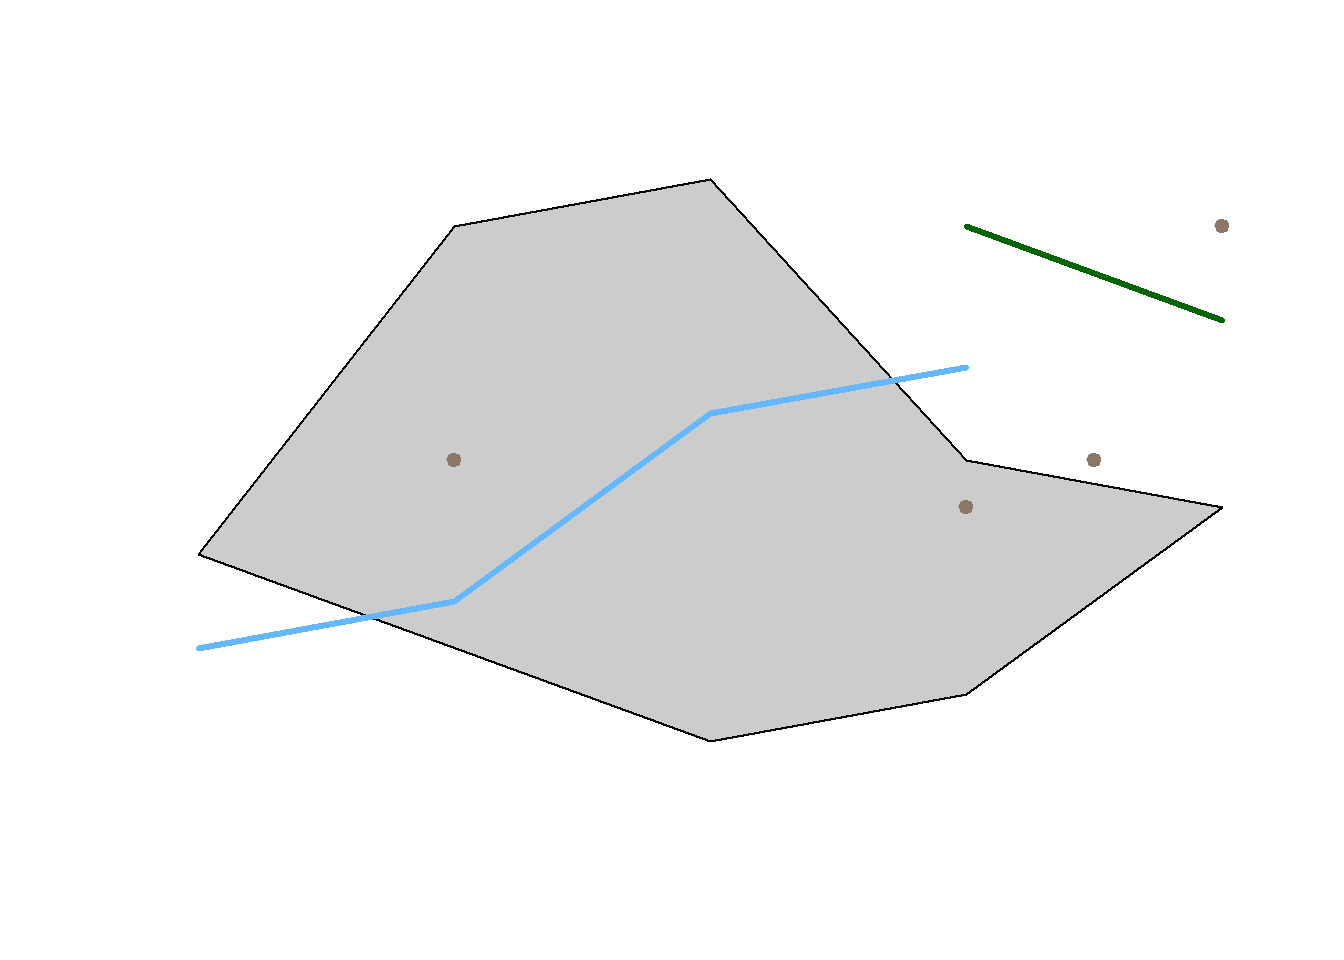
\includegraphics{R-spatial_files/figure-latex/geometric_illustration-1.pdf}

But these are pure geometries defined in the Euclidean space with Cartesian coordinates. we need to refer such data to physical locations on the Earth surface, that is geographically referenced. In order to do that, the software need to know extra information about the shape of the 3D Earth surface and how locations on the 3D surface can be \textbf{\emph{projected}} or \textbf{\emph{transformed}} to 2D surfaces like our paper maps and computer screens. The spatial reference systems or coordinate reference systems (CRS) are the solution, which have been fully developed in Geographic Information Science or Geographic Information Systems.

\begin{quote}
\begin{itemize}
\tightlist
\item
  \emph{In the next session, we will continue to examine some of the details of CRS. In this session, we start to learn how it is defined and used.}
\item
  \emph{Geographic data, by definition, are spatial data with reference to the Earth surface. Spatial data, by contrast, could refer to any surfaces or spaces. In other words, all geographic data are spatial data but some spatial data are not geographic data. While mostly interchangeable, they could usefully differentiate them in some contexts.}
\end{itemize}
\end{quote}

\hypertarget{handling-spatial-data-in-r}{%
\subsection{Handling spatial data in R}\label{handling-spatial-data-in-r}}

Spatial data analysis has always been an important component in the R ecosystem. For vector spatial data in R, there are two families of data structures based on two packages.

\begin{itemize}
\tightlist
\item
  \textbf{\emph{sp} family}: used to be \emph{de facto} standard and still popular

  \begin{itemize}
  \tightlist
  \item
    \emph{sp} means \emph{spatial} and defines a family of spatial data classes.
  \item
    some of the top level classes are SpaitalPointsDataFrame, SpatialMultiPointsDataFrame, SpatialLinesDataFrame, and SpatialPolygonsDataFrame.
  \item
    The ESRI Shapefile is closest to \emph{sp} in terms of data organization.
  \end{itemize}
\item
  \textbf{\emph{sf} family}: the newer and ``modern'' standard

  \begin{itemize}
  \tightlist
  \item
    \emph{sf} means \emph{Simple Feature} as defined by \href{http://www.opengeospatial.org/}{Open Geospatial Consortium or OGC}.
  \item
    It is faster, more efficient, and consistent with other software like PostGIS.
  \item
    \emph{sf} is supported by the R Consortium and therefore ``official.''
  \item
    It is almost the same as the table format in spatial databases like PostGIS and SpatiaLite.
  \item
    \emph{sf} is tidyverse compatible and works well with tidy-packages like \textbf{dplyr}, \textbf{ggplot}, and \textbf{tidycensus}
  \end{itemize}
\end{itemize}

One must understand that \emph{sp} and \emph{sf} are not two rivals in the R ecosystem. Instead, \emph{sf} is more like a natural evolution of \emph{sp}. First, there is demand to \textbf{unify} the data models across the entire geospatial industry so that GIS software and spatial databases are compatible and interoperable. OGC is leading the development of such geospatial standards. Most organizations and products like QGIS, PostGIS, and ArcGIS are increasingly adopting them. And \emph{sf} was a response from the R spatial community to these standards.

Second, R now has more advanced data processing features and better fundamental packages such as those in the \emph{tidyverse}. For geospatial data, more efficient open source spatial libraries also become available based on libraries like RGEOS, GDAL, PROJ, boost geometry etc. The new \emph{sf} package can better take advantage of these developments.

Practically, it is very easy to convert between \emph{sp} and \emph{sf} structures as their underlying spatial models are compatible. And some of the key developers are actually working on both packages. Many R spatial packages can use both. But in case a package can only use one of them, we must make explicit conversions, mostly from \emph{sf} to \emph{sp} because most classic R spatial packages are based on \emph{sp}.

That being said, when and where possible, we should always give the \emph{sf}-family packages a higher priority as most packages are reworking towards being \emph{tidyverse} compatible. Some packages related to the \emph{sp} family packages are retiring. For this course, we focus on the \emph{sf} package.

\hypertarget{the-sf-package}{%
\subsection{\texorpdfstring{The \emph{sf} package}{The sf package}}\label{the-sf-package}}

The \href{https://cran.r-project.org/package=sf}{\emph{sf}}\footnote{E. Pebesma \& R. Bivand (2016)\href{http://pebesma.staff.ifgi.de/pebesma_sfr.pdf}{Spatial data in R: simple features and
  future perspectives}} package is first released on CRAN in late October 2016 . It implements a formal standard called \href{https://en.wikipedia.org/wiki/Simple_Features}{``Simple Features''} that specifies a storage and access model of spatial geometries such as points, lines, and polygons. A feature geometry is called simple when it meets certain criteria. For example, simple polygons cannot self-intersecting and they cannot have spikes or dangling vetexes. Simple Features are independent and have no explicit information about their neighbors or other spatially connected features. This standard has been adopted widely, not only by spatial databases such as PostGIS, but also web standards such as GeoJSON.

If you work with PostGIS or GeoJSON you may have come across the \href{https://en.wikipedia.org/wiki/Well-known_text}{WKT (well-known text)} format (Fig 1.1 and 1.2). Note that these texts are not what are being actually saved or encoded in the data. They are just for users' convenience as they are readable as opposed to the binary code.

\begin{figure}
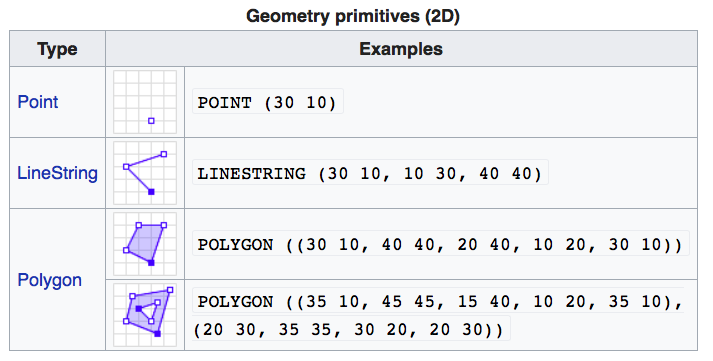
\includegraphics[width=1\linewidth]{img/wkt_primitives} \caption{Well-Known-Text Geometry primitives  (wikipedia)}\label{fig:wkt-primitives-sp}
\end{figure}

\begin{figure}
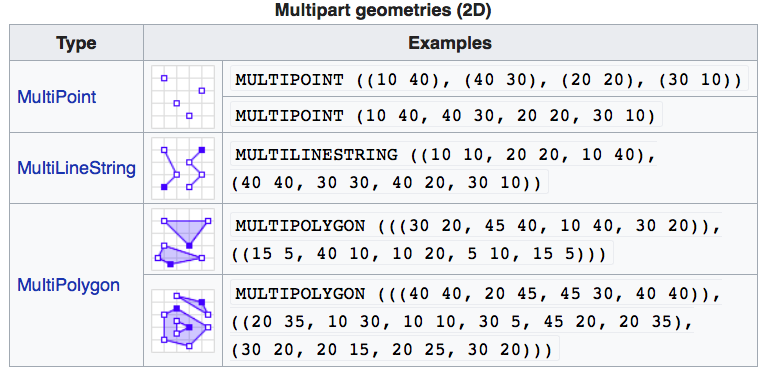
\includegraphics[width=1\linewidth]{img/wkt_multipart} \caption{Well-Known-Text Multipart geometries (wikipedia)}\label{fig:wkt-multipart-sp}
\end{figure}

\emph{sf} implements the Simple Features standard natively in R. \emph{sf} stores spatial objects as a simple data frame with a special column that contains the information for the geometry coordinates. That special column is a list with the same length as the number of rows in the data frame. Each of the individual list elements then can be of any length needed to hold the coordinates that correspond to an individual feature.

\begin{quote}
\textbf{How simple features in R are organized}

The three classes used to represent simple features are:

\begin{itemize}
\tightlist
\item
  \textbf{\emph{sf}}, the table (\textbf{\emph{data.frame}}) with feature attributes and feature geometries, which contains
\item
  \textbf{\emph{sfc}}, the list-column with the geometries for each feature (record), which is composed of
\item
  \textbf{\emph{sfg}}, the feature geometry of an individual simple feature.
\end{itemize}
\end{quote}

\begin{figure}
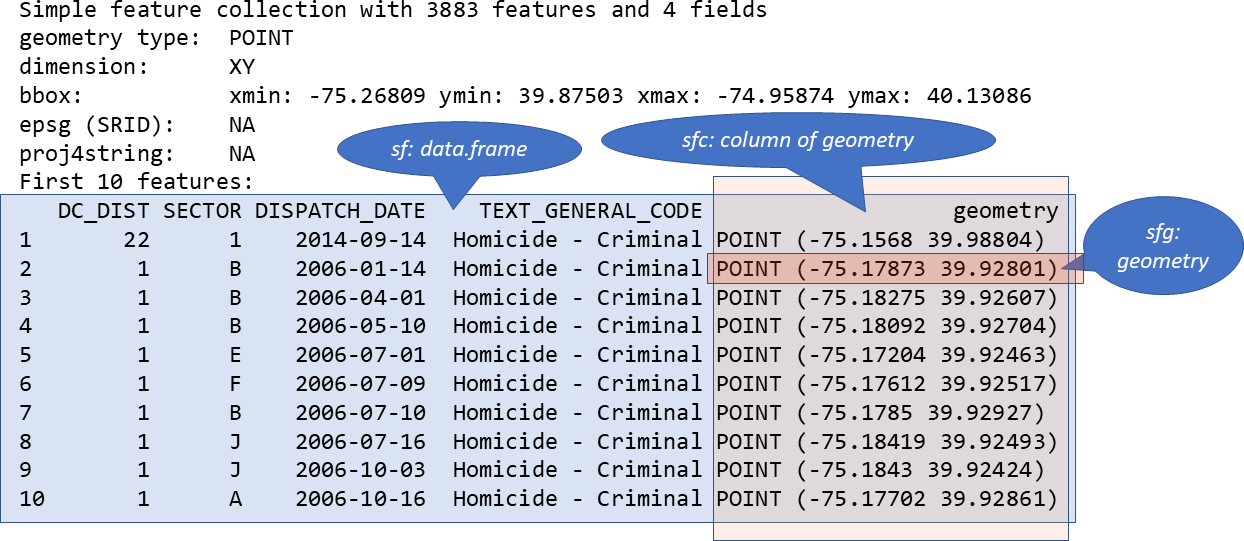
\includegraphics[width=1\linewidth]{img/sf_sfc_sfg} \caption{Relationship of sf, sfc, and sfg}\label{fig:sf-sfc-sfg}
\end{figure}

\hypertarget{create-a-spatial-sf-object-manually}{%
\subsection{\texorpdfstring{Create a spatial \emph{sf} object manually}{Create a spatial sf object manually}}\label{create-a-spatial-sf-object-manually}}

The basic steps of creating \emph{sf} objects are bottom-up, that is from \emph{sfg}, to \emph{sfc}, then to \emph{sf}.

\begin{quote}
I. Create geometric objects
\end{quote}

Geometric objects (simple features) can be created from a numeric vector, matrix or a list with the coordinates. They are called \emph{sfg} objects for Simple Feature Geometry. In \emph{sf} package, there are functions that help create simple feature geometries, like \texttt{st\_point()}, \texttt{st\_linestring()}, \texttt{st\_polygon()} and more.

\begin{quote}
\begin{enumerate}
\def\labelenumi{\Roman{enumi}.}
\setcounter{enumi}{1}
\tightlist
\item
  Combine all individual single feature objects for the special column.
\end{enumerate}
\end{quote}

The feature geometries are then combined into a Simple Feature Collection with \texttt{st\_sfc()}. which is nothing other than a simple feature geometry list-column. The \emph{sfc} object also holds the bounding box and the projection information.

\begin{quote}
\begin{enumerate}
\def\labelenumi{\Roman{enumi}.}
\setcounter{enumi}{2}
\tightlist
\item
  Add attributes.
\end{enumerate}
\end{quote}

Lastly, we add the attributes to the the simple feature collection with the \texttt{st\_sf()} function. This function extends the well known data frame in R with a column that holds the simple feature collection.

Here we try to creat some highway objects. First, we would generate LINESTRINGs as simple feature geometries \emph{sfg} out of a matrix with coordinates:

\begin{Shaded}
\begin{Highlighting}[]
\FunctionTok{set.seed}\NormalTok{(}\DecValTok{1006}\NormalTok{) }\CommentTok{\# for replicability}
\CommentTok{\# runif(6) generates 6 random numbers in uniform distribution}
\NormalTok{lnstr\_sfg1 }\OtherTok{\textless{}{-}} \FunctionTok{st\_linestring}\NormalTok{(}\FunctionTok{matrix}\NormalTok{(}\FunctionTok{runif}\NormalTok{(}\DecValTok{6}\NormalTok{), }\AttributeTok{ncol=}\DecValTok{2}\NormalTok{)) }
\FunctionTok{set.seed}\NormalTok{(}\DecValTok{1043}\NormalTok{)}
\NormalTok{lnstr\_sfg2 }\OtherTok{\textless{}{-}} \FunctionTok{st\_linestring}\NormalTok{(}\FunctionTok{matrix}\NormalTok{(}\FunctionTok{runif}\NormalTok{(}\DecValTok{6}\NormalTok{), }\AttributeTok{ncol=}\DecValTok{2}\NormalTok{)) }
\FunctionTok{class}\NormalTok{(lnstr\_sfg1)}
\end{Highlighting}
\end{Shaded}

\begin{verbatim}
#> [1] "XY"         "LINESTRING" "sfg"
\end{verbatim}

We would then combine this into a simple feature collection \emph{sfc}:

\begin{Shaded}
\begin{Highlighting}[]
\NormalTok{lnstr\_sfc }\OtherTok{\textless{}{-}} \FunctionTok{st\_sfc}\NormalTok{(lnstr\_sfg1, lnstr\_sfg2) }\CommentTok{\# just one feature here}
\FunctionTok{class}\NormalTok{(lnstr\_sfc)}
\end{Highlighting}
\end{Shaded}

\begin{verbatim}
#> [1] "sfc_LINESTRING" "sfc"
\end{verbatim}

And lastly use our data frame from above to generate the \emph{sf} object:

\begin{Shaded}
\begin{Highlighting}[]
\NormalTok{dfr }\OtherTok{\textless{}{-}} \FunctionTok{data.frame}\NormalTok{(}\AttributeTok{id =} \FunctionTok{c}\NormalTok{(}\StringTok{"hwy1"}\NormalTok{, }\StringTok{"hwy2"}\NormalTok{), }\AttributeTok{cars\_per\_hour =} \FunctionTok{c}\NormalTok{(}\DecValTok{78}\NormalTok{, }\DecValTok{22}\NormalTok{)) }
\NormalTok{lnstr\_sf }\OtherTok{\textless{}{-}} \FunctionTok{st\_sf}\NormalTok{(dfr , lnstr\_sfc)}
\FunctionTok{class}\NormalTok{(lnstr\_sf)}
\end{Highlighting}
\end{Shaded}

\begin{verbatim}
#> [1] "sf"         "data.frame"
\end{verbatim}

\begin{Shaded}
\begin{Highlighting}[]
\FunctionTok{plot}\NormalTok{(lnstr\_sf, }\AttributeTok{col=}\StringTok{\textquotesingle{}black\textquotesingle{}}\NormalTok{)}
\end{Highlighting}
\end{Shaded}

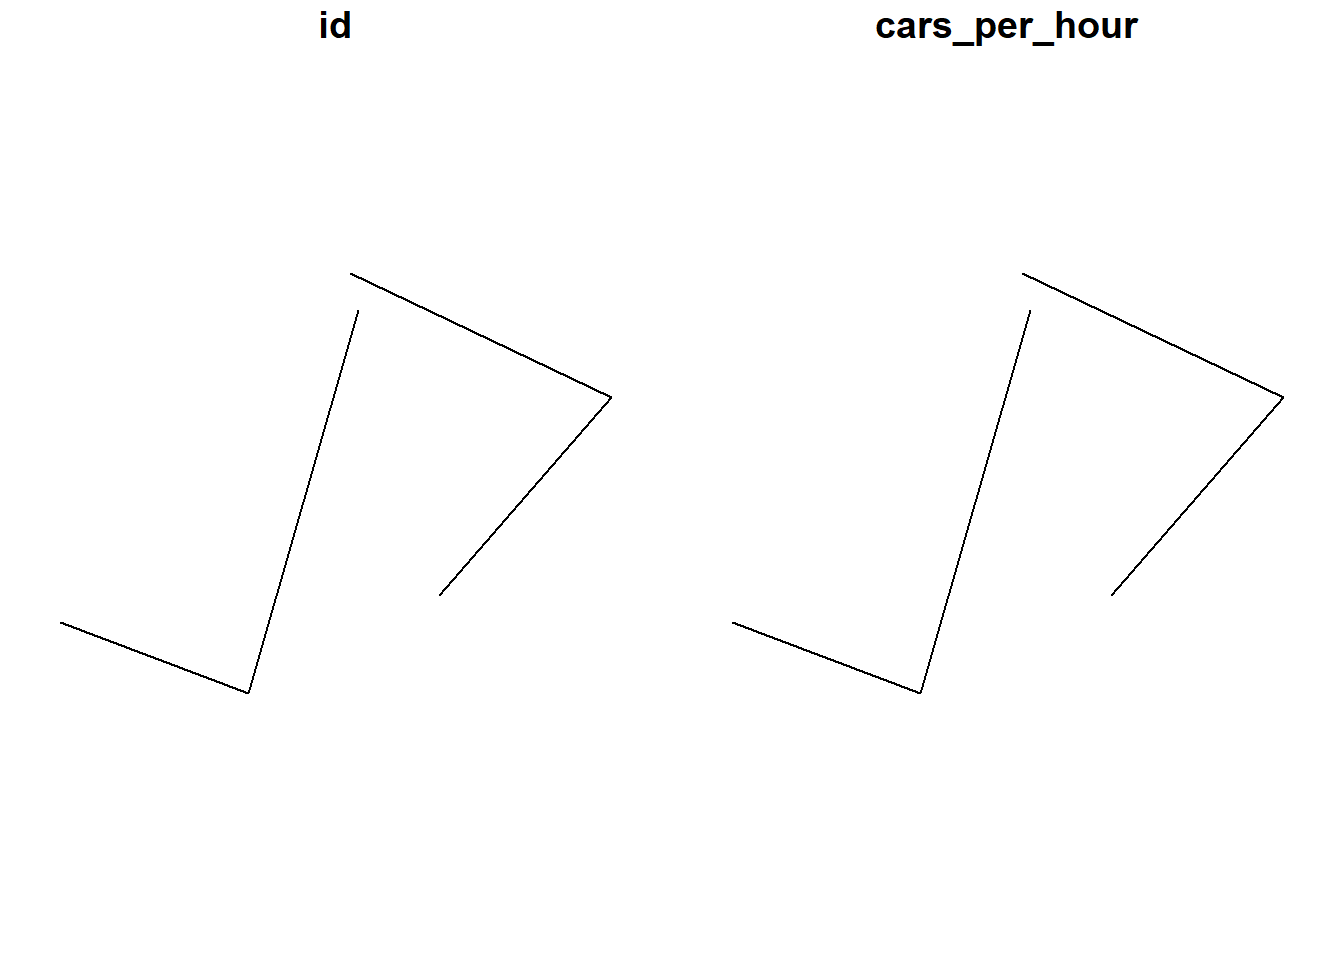
\includegraphics{R-spatial_files/figure-latex/sf-line-plot-1.pdf}

\hypertarget{sf-methods}{%
\subsection{\texorpdfstring{\emph{sf} methods}{sf methods}}\label{sf-methods}}

There are many methods available in the \emph{sf} package. Most function names, particularly those related to spatial data processing and analysis, start with \textbf{\texttt{st\_}}, which means \textbf{\emph{S}}patial \textbf{\emph{T}}ype. To find out more, use

\begin{Shaded}
\begin{Highlighting}[]
\FunctionTok{methods}\NormalTok{(}\AttributeTok{class=}\StringTok{"sf"}\NormalTok{)}
\end{Highlighting}
\end{Shaded}

\begin{verbatim}
#>   [1] $<-                   [                     [[<-                 
#>   [4] aggregate             anti_join             arrange              
#>   [7] as.data.frame         cbind                 coerce               
#>  [10] dbDataType            dbWriteTable          distinct             
#>  [13] dplyr_reconstruct     extent                extract              
#>  [16] filter                full_join             gather               
#>  [19] group_by              group_split           identify             
#>  [22] initialize            inner_join            left_join            
#>  [25] mapView               mask                  merge                
#>  [28] mutate                nest                  pivot_longer         
#>  [31] plot                  print                 raster               
#>  [34] rasterize             rbind                 rename               
#>  [37] right_join            rowwise               sample_frac          
#>  [40] sample_n              select                semi_join            
#>  [43] separate              separate_rows         show                 
#>  [46] slice                 slotsFromS3           spread               
#>  [49] st_agr                st_agr<-              st_area              
#>  [52] st_as_s2              st_as_sf              st_as_sfc            
#>  [55] st_bbox               st_boundary           st_buffer            
#>  [58] st_cast               st_centroid           st_collection_extract
#>  [61] st_convex_hull        st_coordinates        st_crop              
#>  [64] st_crs                st_crs<-              st_difference        
#>  [67] st_drop_geometry      st_filter             st_geometry          
#>  [70] st_geometry<-         st_inscribed_circle   st_interpolate_aw    
#>  [73] st_intersection       st_intersects         st_is                
#>  [76] st_is_valid           st_join               st_line_merge        
#>  [79] st_m_range            st_make_valid         st_nearest_points    
#>  [82] st_node               st_normalize          st_point_on_surface  
#>  [85] st_polygonize         st_precision          st_reverse           
#>  [88] st_sample             st_segmentize         st_set_precision     
#>  [91] st_shift_longitude    st_simplify           st_snap              
#>  [94] st_sym_difference     st_transform          st_triangulate       
#>  [97] st_union              st_voronoi            st_wrap_dateline     
#> [100] st_write              st_z_range            st_zm                
#> [103] summarise             transform             transmute            
#> [106] ungroup               unite                 unnest               
#> see '?methods' for accessing help and source code
\end{verbatim}

Here are some of the other highlights of \emph{sf} that you might be interested in:

\begin{itemize}
\item
  provides \textbf{fast} I/O, particularly relevant for large files
\item
  spatial functions that rely on GEOS and GDAL and PROJ external libraries are directly linked into the package, so no need to load additional external packages (like in \emph{sp})\\
\item
  \emph{sf} objects can be plotted directly with \texttt{ggplot}
\item
  \emph{sf} directly reads from and writes to spatial \textbf{databases} such as PostGIS
\item
  \emph{sf} is compatible with the \href{https://www.tidyverse.org/}{\texttt{tidyvderse}}, (but see some \href{https://geocompr.github.io/geocompkg/articles/tidyverse-pitfalls.html}{pitfalls here})
\end{itemize}

Note that \emph{sp} and \emph{sf} are not the only way spatial objects are conceptualized in R. Other spatial packages may use their own class definitions for spatial data (for example \texttt{spatstat}).

There are packages specifically for the \href{https://tools.ietf.org/html/rfc7946}{GeoJSON} and for that reason are more lightweight, for example:

\begin{itemize}
\tightlist
\item
  \href{https://cran.r-project.org/package=geojson}{\texttt{geojson}} and\\
\item
  \href{https://CRAN.R-project.org/package=geoops}{\texttt{geoops}} - (\href{https://cran.r-project.org/web/packages/geoops/vignettes/geoops_vignette.html}{demo})
\end{itemize}

Usually you can find functions that convert objects to and from these formats.

\begin{quote}
Self-Exercise

Similarly to the example above generate a Point object in R.

\begin{enumerate}
\def\labelenumi{\arabic{enumi}.}
\tightlist
\item
  Create a matrix \textbf{\emph{pts}} of random numbers with two columns and as many rows as you like. These are your points.
\item
  Create a dataframe \textbf{\emph{attrib\_df}} with the same number of rows as your \textbf{\emph{pts}} matrix and a column that holds an attribute. You can make up any attribute.
\item
  Use the appropriate commands and \textbf{\emph{pts}} to create an \textbf{\emph{sf}} object with a geometry column of class \textbf{\emph{sfc\_POINT}}.
\item
  Try to subset/filter your spatial object using the attribute you have added and the way you are used to from regular data frames.
\item
  How do you determine the bounding box of your spatial object?
\end{enumerate}
\end{quote}

\hypertarget{load-and-display-data-with-sf}{%
\section{\texorpdfstring{Load and Display Data with \emph{sf}}{Load and Display Data with sf}}\label{load-and-display-data-with-sf}}

With good understanding of the \emph{sf} data structure, we are ready to load and display some real data.

\hypertarget{reading-shapefiles-into-r}{%
\subsection{Reading Shapefiles into R}\label{reading-shapefiles-into-r}}

\emph{sf} utilizes the powerful \href{http://gdal.org}{GDAL library} to conduct data I/O (input/output), which is automatically linked in when loading \emph{sf}. GDAL can handle numerous vector and raster data format. The \texttt{st\_read()} method in \emph{sf} is the interface for reading vector spatial data. In this section, we mostly use the Shapefile format.

\begin{Shaded}
\begin{Highlighting}[]
\CommentTok{\# read in a Shapefile. With the \textquotesingle{}shp\textquotesingle{} file extension, sf knows it is a Shapefile.}
\NormalTok{nyc\_sf }\OtherTok{\textless{}{-}} \FunctionTok{st\_read}\NormalTok{(}\StringTok{"data/nyc/nyc\_acs\_tracts.shp"}\NormalTok{)}
\end{Highlighting}
\end{Shaded}

\begin{verbatim}
#> Reading layer `nyc_acs_tracts' from data source 
#>   `D:\Cloud_Drive\Dropbox (Hunter College)\Workspace\RSpace\R-Spatial_Book\data\nyc\nyc_acs_tracts.shp' 
#>   using driver `ESRI Shapefile'
#> Simple feature collection with 2166 features and 113 fields
#> Geometry type: MULTIPOLYGON
#> Dimension:     XY
#> Bounding box:  xmin: -74.25559 ymin: 40.49612 xmax: -73.70001 ymax: 40.91553
#> Geodetic CRS:  NAD83
\end{verbatim}

\begin{Shaded}
\begin{Highlighting}[]
\CommentTok{\# take a look at what we\textquotesingle{}ve got}
\FunctionTok{str}\NormalTok{(nyc\_sf) }\CommentTok{\# note again the geometry column at the end of the output}
\end{Highlighting}
\end{Shaded}

\begin{verbatim}
#> Classes 'sf' and 'data.frame':   2166 obs. of  114 variables:
#>  $ UNEMP_RATE: num  0 0.0817 0.1706 0 0.088 ...
#>  $ cartodb_id: num  1 2 3 4 5 6 7 8 9 10 ...
#>  $ withssi   : int  0 228 658 0 736 0 261 0 39 638 ...
#>  $ withsocial: int  0 353 1577 0 1382 99 1122 10 264 895 ...
#>  $ withpubass: int  0 47 198 0 194 0 145 0 5 334 ...
#>  $ struggling: int  0 694 2589 0 2953 337 3085 17 131 1938 ...
#>  $ profession: int  0 0 36 0 19 745 18 49 35 0 ...
#>  $ popunemplo: int  0 92 549 0 379 321 432 26 106 494 ...
#>  $ poptot    : int  0 2773 8339 0 10760 7024 10955 849 1701 5923 ...
#>  $ popover18 : int  0 2351 6878 0 8867 6637 8932 711 1241 4755 ...
#>  $ popinlabou: int  0 1126 3218 0 4305 5702 5114 657 735 2283 ...
#>  $ poororstru: int  0 2026 4833 0 7044 1041 6376 112 232 4115 ...
#>  $ poor      : int  0 1332 2244 0 4091 704 3291 95 101 2177 ...
#>  $ pacificune: int  0 0 0 0 13 0 0 0 0 0 ...
#>  $ pacificinl: int  0 0 0 0 13 0 0 0 0 0 ...
#>  $ pacific   : int  0 0 0 0 13 0 0 0 0 0 ...
#>  $ otherunemp: int  0 0 103 0 46 0 0 0 17 151 ...
#>  $ otherinlab: int  0 144 348 0 609 112 184 48 90 525 ...
#>  $ otherethni: int  0 598 1175 0 1799 112 377 48 183 1664 ...
#>  $ onlyprofes: int  0 0 102 0 20 890 116 78 77 0 ...
#>  $ onlymaster: int  0 77 412 0 292 2162 408 233 328 16 ...
#>  $ onlylessth: int  0 878 2164 0 3793 121 4384 34 115 1846 ...
#>  $ onlyhighsc: int  0 1088 4068 0 3868 5508 3882 631 1093 2343 ...
#>  $ onlydoctor: int  0 0 66 0 1 145 98 29 42 0 ...
#>  $ onlycolleg: int  0 471 2355 0 2290 5371 2223 585 884 1111 ...
#>  $ onlybachel: int  0 271 1269 0 1322 4685 1262 481 687 200 ...
#>  $ okay      : int  0 742 3474 0 3499 5982 4579 733 1469 1798 ...
#>  $ mixedunemp: int  0 16 21 0 14 24 0 0 51 31 ...
#>  $ mixedinlab: int  0 72 134 0 100 136 91 10 62 140 ...
#>  $ mixed     : int  0 175 234 0 251 224 115 16 102 334 ...
#>  $ master    : int  0 77 310 0 272 1272 292 155 251 16 ...
#>  $ maleunempl: int  0 76 349 0 179 204 197 8 72 277 ...
#>  $ maleover18: int  0 1101 3134 0 4068 3557 3992 454 613 1935 ...
#>  $ malepro   : int  0 0 36 0 19 473 48 51 61 0 ...
#>  $ malemastr : int  0 10 143 0 126 1034 181 123 139 0 ...
#>  $ male_lesHS: int  0 302 1063 0 1693 29 2013 17 103 714 ...
#>  $ male_HS   : int  0 607 1893 0 1651 2985 1702 414 485 985 ...
#>  $ male_doctr: int  0 0 24 0 0 77 30 29 38 0 ...
#>  $ male_collg: int  0 227 1225 0 997 2924 871 381 368 462 ...
#>  $ male_BA   : int  0 132 668 0 562 2411 499 288 292 43 ...
#>  $ maleinlabo: int  0 612 1640 0 2059 3299 2466 423 392 991 ...
#>  $ maledrop  : int  0 16 8 0 0 0 0 0 0 0 ...
#>  $ male16to19: int  0 65 253 0 162 37 236 20 32 187 ...
#>  $ male      : int  0 1318 3850 0 4796 3840 5244 533 897 2514 ...
#>  $ lessthanhi: int  0 878 2164 0 3793 121 4384 34 115 1846 ...
#>  $ lessthan10: int  0 212 760 0 1100 289 625 2 51 463 ...
#>  $ households: int  0 986 3382 0 3838 4104 3950 367 739 2224 ...
#>  $ hispanicun: int  0 30 269 0 115 27 0 0 68 335 ...
#>  $ hispanicin: int  0 357 1171 0 819 297 236 77 201 1145 ...
#>  $ hispanic  : int  0 1187 3503 0 2608 374 318 108 360 3478 ...
#>  $ highschool: int  0 617 1713 0 1578 137 1659 46 209 1232 ...
#>  $ geo_state : int  36 36 36 36 36 36 36 36 36 36 ...
#>  $ geo_place : int  51000 51000 51000 51000 51000 51000 51000 51000 51000 51000 ...
#>  $ geo_county: int  61 61 61 61 61 61 61 61 61 61 ...
#>  $ field_1   : int  1 2 3 4 5 6 7 8 9 10 ...
#>  $ femaleunem: int  0 16 200 0 200 117 235 18 34 217 ...
#>  $ femaleover: int  0 1250 3744 0 4799 3080 4940 257 628 2820 ...
#>  $ fem_profes: int  0 0 66 0 1 417 68 27 16 0 ...
#>  $ fem_master: int  0 67 269 0 166 1128 227 110 189 16 ...
#>  $ fem_lessHS: int  0 576 1101 0 2100 92 2371 17 12 1132 ...
#>  $ fem_HS    : int  0 481 2175 0 2217 2523 2180 217 608 1358 ...
#>  $ fem_doctor: int  0 0 42 0 1 68 68 0 4 0 ...
#>  $ fem_colleg: int  0 244 1130 0 1293 2447 1352 204 516 649 ...
#>  $ fem_BA    : int  0 139 601 0 760 2274 763 193 395 157 ...
#>  $ femaleinla: int  0 514 1578 0 2246 2403 2648 234 343 1292 ...
#>  $ femaledrop: int  0 0 1 0 0 0 0 0 0 14 ...
#>  $ femal16_19: int  0 84 124 0 271 2 126 2 32 242 ...
#>  $ female    : int  0 1455 4489 0 5964 3184 5711 316 804 3409 ...
#>  $ europeanun: int  0 14 328 0 56 188 71 26 22 132 ...
#>  $ europeanin: int  0 303 1641 0 525 4058 492 540 543 510 ...
#>  $ european  : int  0 540 4091 0 1181 4975 929 717 1327 1645 ...
#>  $ doctorate : int  0 0 66 0 1 145 98 29 42 0 ...
#>  $ com_90plus: int  0 49 101 0 36 61 82 17 27 178 ...
#>  $ comm_5less: int  0 99 0 0 1 220 46 26 0 0 ...
#>  $ comm_60_89: int  0 40 215 0 370 136 687 32 41 331 ...
#>  $ comm_5_14 : int  0 121 226 0 331 913 718 87 58 99 ...
#>  $ comm_45_59: int  0 142 171 0 284 287 409 46 84 351 ...
#>  $ comm_30_44: int  0 217 923 0 1442 1514 1118 198 210 493 ...
#>  $ comm_15_29: int  0 352 970 0 1250 1840 1363 192 134 304 ...
#>  $ college   : int  0 200 1086 0 968 686 961 104 197 911 ...
#>  $ bachelor  : int  0 194 857 0 1030 2523 854 248 359 184 ...
#>  $ asianunemp: int  0 62 38 0 207 108 352 0 16 61 ...
#>  $ asianinlab: int  0 559 615 0 2736 1286 4283 42 35 491 ...
#>  $ asian     : int  0 1249 1724 0 6549 1598 9448 51 75 922 ...
#>  $ americanun: int  0 0 0 0 0 1 0 0 0 24 ...
#>  $ americanin: int  0 0 0 0 57 1 0 0 0 24 ...
#>  $ american  : int  0 43 0 0 57 1 0 0 0 51 ...
#>  $ africanune: int  0 0 59 0 43 0 9 0 0 95 ...
#>  $ africaninl: int  0 48 434 0 265 109 64 17 5 593 ...
#>  $ african   : int  0 168 1115 0 910 114 86 17 14 1307 ...
#>  $ puma      : chr  "3810" "3809" "3809" "3810" ...
#>  $ ntaname   : chr  "park-cemetery-etc-Manhattan" "Lower East Side" "Lower East Side" "park-cemetery-etc-Manhattan" ...
#>  $ ntacode   : chr  "MN99" "MN28" "MN28" "MN99" ...
#>  $ ctlabel   : chr  "1" "2.01" "2.02" "5" ...
#>  $ cdeligibil: chr  "I" "E" "E" "I" ...
#>  $ boroname  : chr  "Manhattan" "Manhattan" "Manhattan" "Manhattan" ...
#>  $ medianinco: num  NA 17282 24371 NA 18832 ...
#>  $ medianagem: num  NA 39.3 44.9 NA 43.4 29.7 42 33.2 41.5 31.2 ...
#>  $ medianagef: num  NA 43.8 47.9 NA 43 28.3 43 31.9 45.7 47.5 ...
#>   [list output truncated]
#>  - attr(*, "sf_column")= chr "geometry"
#>  - attr(*, "agr")= Factor w/ 3 levels "constant","aggregate",..: NA NA NA NA NA NA NA NA NA NA ...
#>   ..- attr(*, "names")= chr [1:113] "UNEMP_RATE" "cartodb_id" "withssi" "withsocial" ...
\end{verbatim}

Two more words about the geometry column: The geometry column does not have to be named ``geometry''. You can name this column any way you wish. ``geom'', for example, is another popular name for the geometry column. Secondly, you can remove this column and revert to a regular, non-spatial dataframe at any time with \texttt{st\_drop\_geometry()}.

\hypertarget{simple-sf-plotting}{%
\subsection{\texorpdfstring{Simple \emph{sf} plotting}{Simple sf plotting}}\label{simple-sf-plotting}}

The default \texttt{plot} of an \emph{sf} object is a multi-plot of the first attributes, with a warning if not all can be plotted. By default, it plots the first 9 columns:

In order to only plot the polygon boundaries we need to directly use the geometry column. We use the \texttt{st\_geometry()} function to extract it. We can also select a single column or a few columns to draw.

\begin{Shaded}
\begin{Highlighting}[]
\CommentTok{\# pure geometry}
\FunctionTok{plot}\NormalTok{(}\FunctionTok{st\_geometry}\NormalTok{(nyc\_sf), }\AttributeTok{main=}\StringTok{\textquotesingle{}Pure geometry with st\_geometry function\textquotesingle{}}\NormalTok{)}
\end{Highlighting}
\end{Shaded}

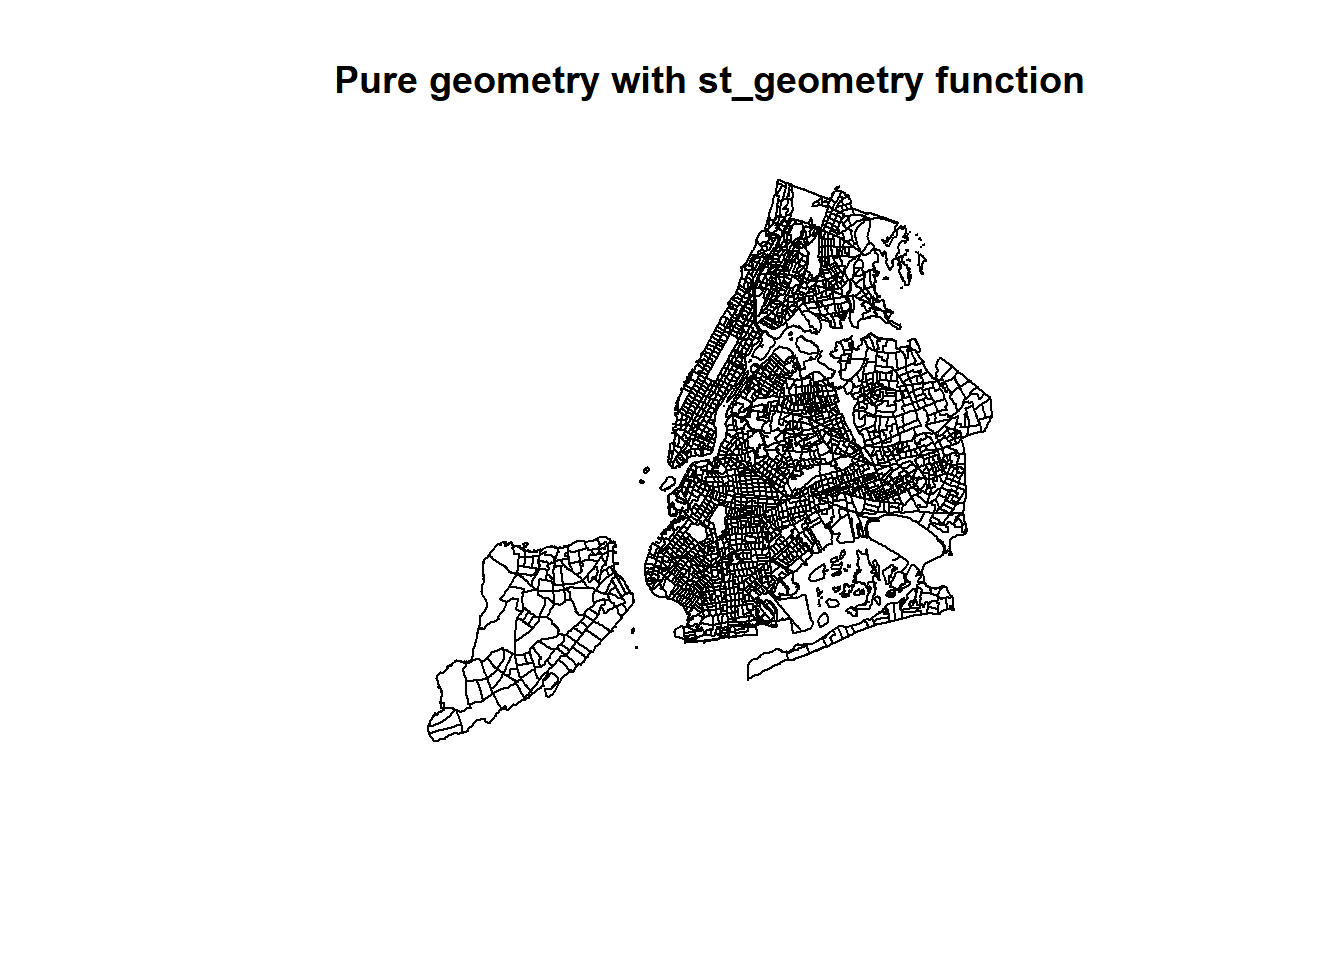
\includegraphics{R-spatial_files/figure-latex/plot-shp-sfg-1.pdf}

\begin{Shaded}
\begin{Highlighting}[]
\CommentTok{\# Only the college column, with geometry}
\FunctionTok{plot}\NormalTok{(nyc\_sf[}\StringTok{\textquotesingle{}college\textquotesingle{}}\NormalTok{], }\AttributeTok{main=}\StringTok{\textquotesingle{}One column with ["college"]\textquotesingle{}}\NormalTok{)}
\end{Highlighting}
\end{Shaded}

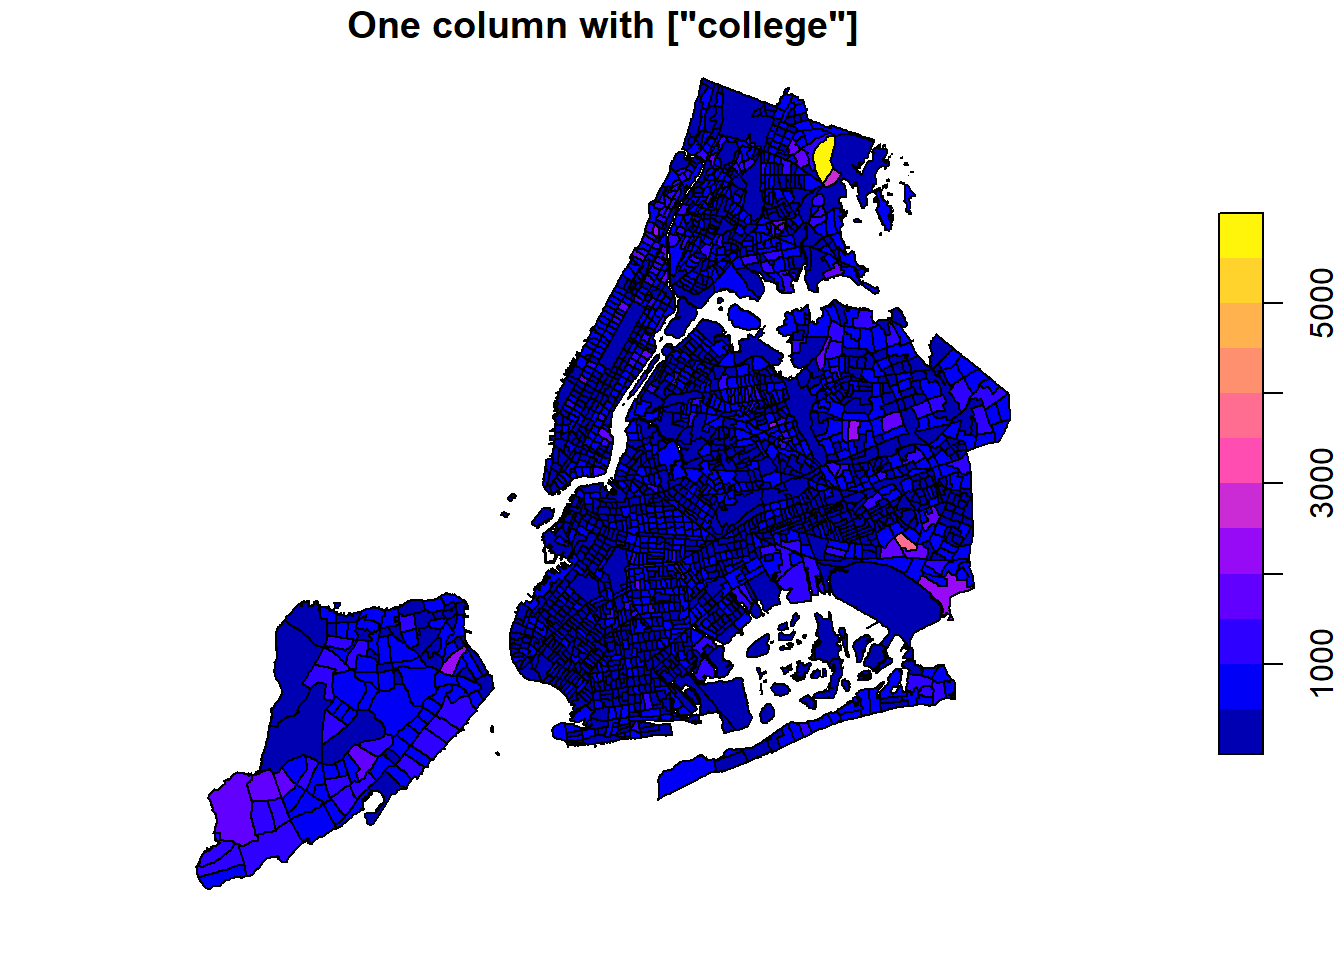
\includegraphics{R-spatial_files/figure-latex/plot-shp-sfg-2.pdf}

\begin{Shaded}
\begin{Highlighting}[]
\CommentTok{\# Two columns, with geometry}
\FunctionTok{plot}\NormalTok{(nyc\_sf[}\FunctionTok{c}\NormalTok{(}\StringTok{\textquotesingle{}college\textquotesingle{}}\NormalTok{, }\StringTok{\textquotesingle{}fem\_colleg\textquotesingle{}}\NormalTok{)], }\AttributeTok{main=}\StringTok{\textquotesingle{}Two Columns with ["college", "fem\_colleg"]\textquotesingle{}}\NormalTok{)}
\end{Highlighting}
\end{Shaded}

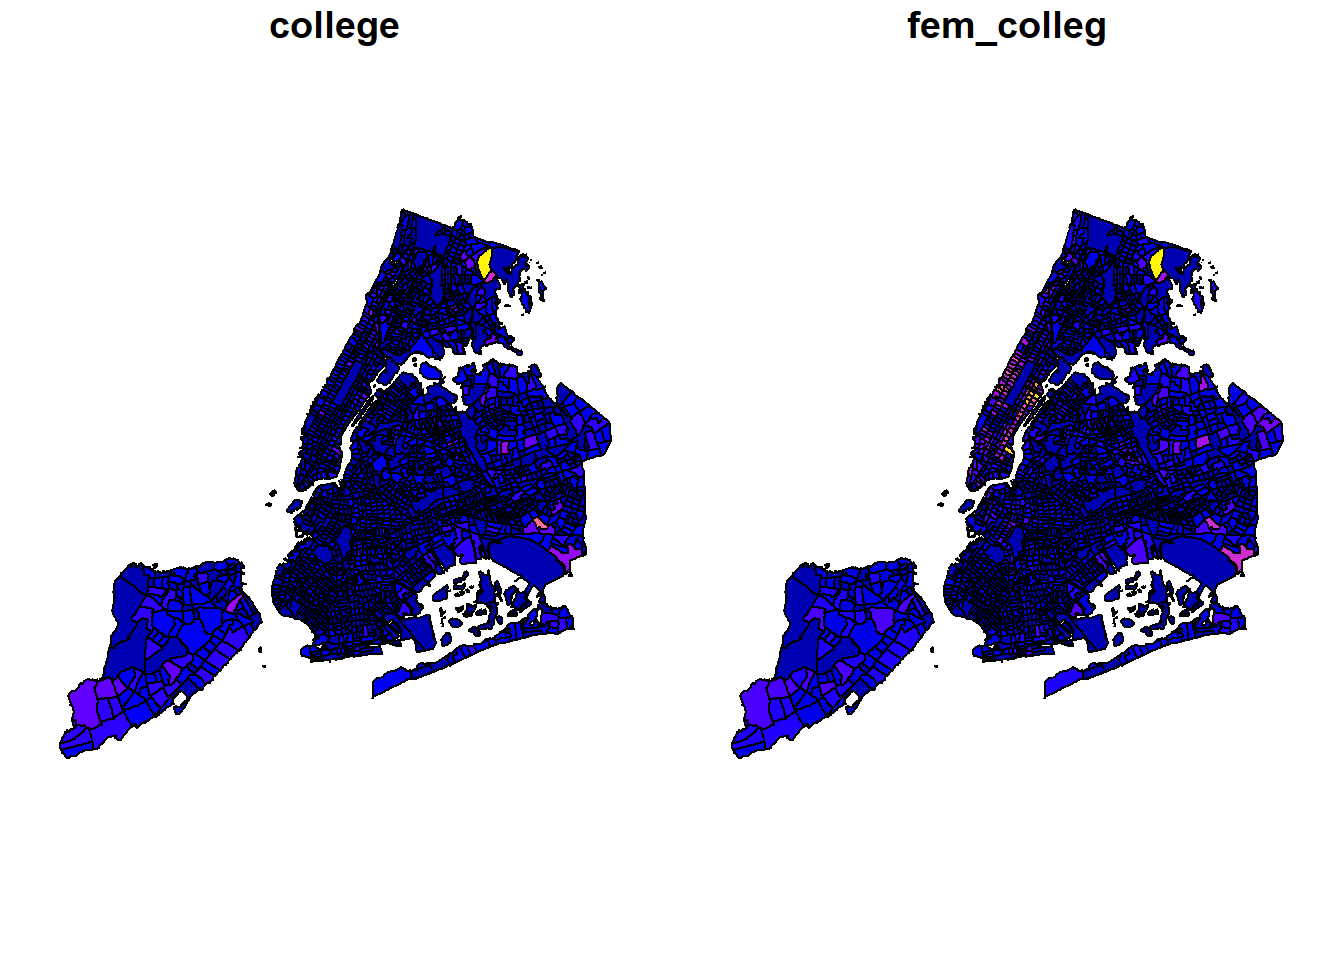
\includegraphics{R-spatial_files/figure-latex/plot-shp-sfg-3.pdf}

Let's add a subset of polygons with only the census tracts where the median household income is more than \$80,000. We can extract elements from an \emph{sf} object based on attributes using your preferred method of filtering dataframes.

\begin{Shaded}
\begin{Highlighting}[]
\CommentTok{\# Make a plot using all tracts, then add the "rich" in red}
\FunctionTok{plot}\NormalTok{(}\FunctionTok{st\_geometry}\NormalTok{(nyc\_sf))}
\FunctionTok{plot}\NormalTok{(}\FunctionTok{st\_geometry}\NormalTok{(nyc\_sf\_rich), }\AttributeTok{add=}\NormalTok{T, }\AttributeTok{col=}\StringTok{"red"}\NormalTok{)}
\end{Highlighting}
\end{Shaded}

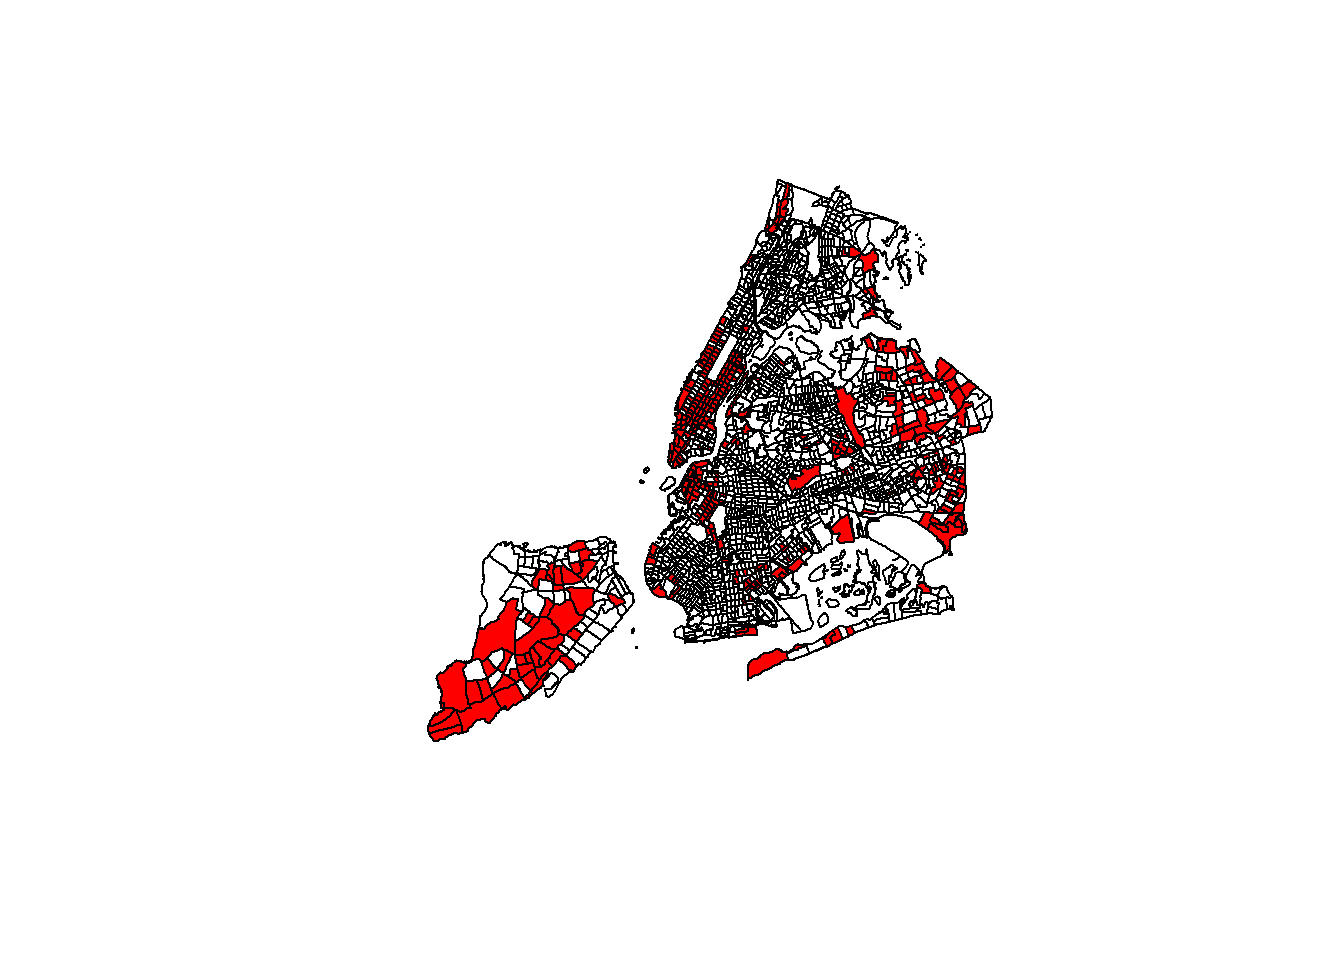
\includegraphics{R-spatial_files/figure-latex/make-subset-plot-shp-sfg-1.pdf}

\textbf{tidyverse} and piping work as well!

\begin{Shaded}
\begin{Highlighting}[]
\FunctionTok{plot}\NormalTok{(nyc\_sf }\SpecialCharTok{\%\textgreater{}\%} \FunctionTok{st\_geometry}\NormalTok{(), }\AttributeTok{col =} \StringTok{\textquotesingle{}NA\textquotesingle{}}\NormalTok{, }\AttributeTok{border=}\StringTok{\textquotesingle{}grey\textquotesingle{}}\NormalTok{, }\AttributeTok{lwd=}\FloatTok{0.5}\NormalTok{)}

\NormalTok{nyc\_sf }\SpecialCharTok{\%\textgreater{}\%} 
  \FunctionTok{filter}\NormalTok{(medianinco }\SpecialCharTok{\textgreater{}} \DecValTok{80000}\NormalTok{) }\SpecialCharTok{\%\textgreater{}\%} 
  \FunctionTok{st\_geometry}\NormalTok{() }\SpecialCharTok{\%\textgreater{}\%} 
  \FunctionTok{plot}\NormalTok{(}\AttributeTok{col=}\StringTok{"red"}\NormalTok{, }\AttributeTok{add=}\NormalTok{T)}
\end{Highlighting}
\end{Shaded}

\hypertarget{simple-interactive-mapping-with-mapview}{%
\subsection{\texorpdfstring{Simple interactive mapping with \emph{mapview}}{Simple interactive mapping with mapview}}\label{simple-interactive-mapping-with-mapview}}

One of most useful, yet simplest methods of visualizing a \emph{sf} object or other spatial data is to utilize the \emph{mapview} package for interactive mapping. \emph{mapview} utilizes the \emph{leaflet} package in R and the original JavaScript \emph{leaflet} library for web mapping. While we will learn the details of \emph{leaflet} later, here is a quick application of the \emph{mapview} package.

\begin{Shaded}
\begin{Highlighting}[]
\CommentTok{\# We use all the default options, but select a few columns. }
\CommentTok{\# If we use all columns, the popup window will be too big. }
\NormalTok{nyc\_sf }\SpecialCharTok{\%\textgreater{}\%}\NormalTok{ dplyr}\SpecialCharTok{::}\FunctionTok{select}\NormalTok{(boroname, poptot, female, doctorate) }\SpecialCharTok{\%\textgreater{}\%}
\NormalTok{  mapview}\SpecialCharTok{::}\FunctionTok{mapview}\NormalTok{()}
\end{Highlighting}
\end{Shaded}

\begin{verbatim}
#> PhantomJS not found. You can install it with webshot::install_phantomjs(). If it is installed, please make sure the phantomjs executable can be found via the PATH variable.
\end{verbatim}

Further configuration could be applied.

\begin{Shaded}
\begin{Highlighting}[]
\NormalTok{nyc\_sf }\SpecialCharTok{\%\textgreater{}\%}\NormalTok{ dplyr}\SpecialCharTok{::}\FunctionTok{select}\NormalTok{(boroname, poptot, female, doctorate) }\OtherTok{{-}\textgreater{}}\NormalTok{ tmp\_sf}

\FunctionTok{mapview}\NormalTok{(tmp\_sf, }\AttributeTok{zcol=}\StringTok{\textquotesingle{}boroname\textquotesingle{}}\NormalTok{, }\AttributeTok{layer.name =} \StringTok{\textquotesingle{}Borough\textquotesingle{}}\NormalTok{, }\AttributeTok{stroke=}\ConstantTok{FALSE}\NormalTok{) }\SpecialCharTok{+} 
  \FunctionTok{mapview}\NormalTok{(tmp\_sf, }\AttributeTok{zcol=}\StringTok{\textquotesingle{}poptot\textquotesingle{}}\NormalTok{, }
          \AttributeTok{layer.name =} \StringTok{\textquotesingle{}Total Population\textquotesingle{}}\NormalTok{, }
          \AttributeTok{homebutton=}\ConstantTok{FALSE}\NormalTok{, }
          \AttributeTok{legend=}\ConstantTok{FALSE}\NormalTok{) }\SpecialCharTok{+}
  \FunctionTok{mapview}\NormalTok{(tmp\_sf, }\AttributeTok{zcol=}\StringTok{"doctorate"}\NormalTok{, }
          \AttributeTok{layer.name =} \StringTok{\textquotesingle{}Population with Doctorate\textquotesingle{}}\NormalTok{, }
          \AttributeTok{homebutton=}\ConstantTok{FALSE}\NormalTok{, }
          \AttributeTok{legend=}\ConstantTok{FALSE}\NormalTok{, }
          \AttributeTok{label=}\StringTok{"doctorate"}\NormalTok{,}
          \AttributeTok{popup =} \StringTok{\textquotesingle{}doctorate\textquotesingle{}}\NormalTok{)}
\end{Highlighting}
\end{Shaded}

\emph{mapview} is particularly suitable for quick and simple interactive mapping. However, the cost of convenience and simplicity is the loss of controls to many details. For example, it is very difficult, if ever possible, to keep the first layer while turning off all other layers using code. With \emph{leaflet}, by contrast, this is an easy task.

\hypertarget{creating-a-spatial-object-from-a-latlon-table}{%
\section{Creating a spatial object from a lat/lon table}\label{creating-a-spatial-object-from-a-latlon-table}}

Increasingly, we are using GPS or GPS-compatible devices to collect spatial data or geographically referenced data in the field. Such data are often organized in a spreadsheet that contains latitude, longitude and some attribute values. We have learned many different ways of reading such spreadsheet into a dataframe. We can then very easily convert the table into a spatial object in R.

\hypertarget{with-sf}{%
\subsection{\texorpdfstring{With \emph{sf}}{With sf}}\label{with-sf}}

An \emph{sf} object can be created from a data frame in the following way. We take advantage of the \texttt{st\_as\_sf()} function which converts any foreign object into an \emph{sf} object. Similarly to above, it requires an argument \texttt{coords}, which in the case of point data needs to be a vector that specifies the dataframe's columns for the longitude and latitude (x,y) coordinates.

\begin{verbatim}
`my_sf_object <- st_as_sf(myDataframe, coords)`
\end{verbatim}

\texttt{st\_as\_sf()} creates a new object and leaves the original data frame untouched.

We use \texttt{read\_csv()} in the \texttt{readr} package to read \texttt{manhattan\_noise.csv} into a dataframe in R and name it \texttt{manhattan\_noise\_df}. Alternatively, we can use the \texttt{read.csv()} in the base package.

\begin{Shaded}
\begin{Highlighting}[]
\CommentTok{\# read\_csv has better capabilities for data types like datetime.}
\NormalTok{manhattan\_noise\_df }\OtherTok{\textless{}{-}} \FunctionTok{read\_csv}\NormalTok{(}\StringTok{"data/nyc/manhattan\_noise.csv"}\NormalTok{, }
                               \AttributeTok{show\_col\_types =} \ConstantTok{FALSE}\NormalTok{, }
                               \AttributeTok{lazy =} \ConstantTok{FALSE}\NormalTok{) }\SpecialCharTok{\%\textgreater{}\%}
\NormalTok{  dplyr}\SpecialCharTok{::}\FunctionTok{mutate}\NormalTok{(}\AttributeTok{datetime =}\NormalTok{ lubridate}\SpecialCharTok{::}\FunctionTok{force\_tz}\NormalTok{(datetime, }\StringTok{\textquotesingle{}America/New\_York\textquotesingle{}}\NormalTok{))}

\CommentTok{\#manhattan\_noise\_df \textless{}{-} read.csv("data/nyc/manhattan\_noise.csv")}
\FunctionTok{str}\NormalTok{(manhattan\_noise\_df)}
\end{Highlighting}
\end{Shaded}

\begin{verbatim}
#> tibble [68,582 x 7] (S3: tbl_df/tbl/data.frame)
#>  $ datetime              : POSIXct[1:68582], format: "2020-07-25 15:02:08" "2020-07-25 02:58:27" ...
#>  $ descriptor            : chr [1:68582] "Loud Music/Party" "Loud Music/Party" "Loud Music/Party" "Loud Music/Party" ...
#>  $ incident_zip          : num [1:68582] 10040 10031 10034 10034 10003 ...
#>  $ incident_address      : chr [1:68582] "281 WADSWORTH AVENUE" "600 WEST  142 STREET" "33 INDIAN ROAD" "65 VERMILYEA AVENUE" ...
#>  $ open_data_channel_type: chr [1:68582] "MOBILE" "ONLINE" "ONLINE" "ONLINE" ...
#>  $ latitude              : num [1:68582] 40.9 40.8 40.9 40.9 40.7 ...
#>  $ longitude             : num [1:68582] -73.9 -74 -73.9 -73.9 -74 ...
\end{verbatim}

\begin{quote}
In the real world, things would not be so smooth as many do not have appropriate knowledge on geography and GPS. Quite often, the coordinate columns are not ready for direct conversion. Commonly problems include:

\begin{itemize}
\tightlist
\item
  coordinates are in degree, minute, and second format instead of decimal degrees.
\item
  The +/- signs in coordinates are replaced by N(orth), S(outh), W(est), E(ast).
\item
  Longitude and latitude are switched or labeled the wrong way.
\item
  Missing the negative signs in coordinates when there should be.
\item
  Coordinates are mixed with text values.
\end{itemize}

With general data processing power in R, these issues can be fixed relatively easily.
\end{quote}

We convert the \texttt{manhattan\_noise\_df} data frame into an \emph{sf} object with \texttt{st\_as\_sf()}

\begin{Shaded}
\begin{Highlighting}[]
\CommentTok{\# Note the two columns for coords must exist in the dataframe}
\NormalTok{manhattan\_noise\_sf }\OtherTok{\textless{}{-}} \FunctionTok{st\_as\_sf}\NormalTok{(manhattan\_noise\_df, }
                               \AttributeTok{coords =} \FunctionTok{c}\NormalTok{(}\StringTok{"longitude"}\NormalTok{, }\StringTok{"latitude"}\NormalTok{))}
\FunctionTok{str}\NormalTok{(manhattan\_noise\_sf)}
\end{Highlighting}
\end{Shaded}

\begin{verbatim}
#> sf [68,582 x 6] (S3: sf/tbl_df/tbl/data.frame)
#>  $ datetime              : POSIXct[1:68582], format: "2020-07-25 15:02:08" "2020-07-25 02:58:27" ...
#>  $ descriptor            : chr [1:68582] "Loud Music/Party" "Loud Music/Party" "Loud Music/Party" "Loud Music/Party" ...
#>  $ incident_zip          : num [1:68582] 10040 10031 10034 10034 10003 ...
#>  $ incident_address      : chr [1:68582] "281 WADSWORTH AVENUE" "600 WEST  142 STREET" "33 INDIAN ROAD" "65 VERMILYEA AVENUE" ...
#>  $ open_data_channel_type: chr [1:68582] "MOBILE" "ONLINE" "ONLINE" "ONLINE" ...
#>  $ geometry              :sfc_POINT of length 68582; first list element:  'XY' num [1:2] -73.9 40.9
#>  - attr(*, "sf_column")= chr "geometry"
#>  - attr(*, "agr")= Factor w/ 3 levels "constant","aggregate",..: NA NA NA NA NA
#>   ..- attr(*, "names")= chr [1:5] "datetime" "descriptor" "incident_zip" "incident_address" ...
\end{verbatim}

Note the additional \textbf{geometry} list-column which now holds the simple feature collection with the coordinates of all the points.

To make it a complete geographical object we assign the WGS84 projection, which has the EPSG code 4326:

\begin{Shaded}
\begin{Highlighting}[]
\FunctionTok{st\_crs}\NormalTok{(manhattan\_noise\_sf)}
\end{Highlighting}
\end{Shaded}

\begin{verbatim}
#> Coordinate Reference System: NA
\end{verbatim}

\begin{Shaded}
\begin{Highlighting}[]
\FunctionTok{st\_crs}\NormalTok{(manhattan\_noise\_sf) }\OtherTok{\textless{}{-}} \DecValTok{4326} \CommentTok{\# we can use EPSG as numeric here}
\CommentTok{\# Alternatively, we can use the sf::st\_set\_crs method}
\CommentTok{\# st\_set\_crs(philly\_homicides\_sf, 4326)}
\FunctionTok{st\_crs}\NormalTok{(manhattan\_noise\_sf)}
\end{Highlighting}
\end{Shaded}

\begin{verbatim}
#> Coordinate Reference System:
#>   User input: EPSG:4326 
#>   wkt:
#> GEOGCRS["WGS 84",
#>     DATUM["World Geodetic System 1984",
#>         ELLIPSOID["WGS 84",6378137,298.257223563,
#>             LENGTHUNIT["metre",1]]],
#>     PRIMEM["Greenwich",0,
#>         ANGLEUNIT["degree",0.0174532925199433]],
#>     CS[ellipsoidal,2],
#>         AXIS["geodetic latitude (Lat)",north,
#>             ORDER[1],
#>             ANGLEUNIT["degree",0.0174532925199433]],
#>         AXIS["geodetic longitude (Lon)",east,
#>             ORDER[2],
#>             ANGLEUNIT["degree",0.0174532925199433]],
#>     USAGE[
#>         SCOPE["Horizontal component of 3D system."],
#>         AREA["World."],
#>         BBOX[-90,-180,90,180]],
#>     ID["EPSG",4326]]
\end{verbatim}

\begin{quote}
\begin{itemize}
\tightlist
\item
  Geographic coordinates from GPS are always using the WGS84 projection, which has a EPSG code of 4326.
\item
  EPSG stands for European Petroleum Survey Group. The map projections are too complicated for many engineers in the petroleum industry. So they started using numeric codes, SRID, to denote spatial reference systems (SRS). Such simplicity has also been favored by software engineers, so they also use EPSG extensively. By contrast, GIS professionals and users are supposedly to have good knowledge on map projection and reference systems. As a result, classic GIS software like ArcGIS have just started using EPSG codes.\\
\item
  There are many websites that allow us to query EPSG codes. The best one, in my opinion, is \href{https://spatialreference.org/}{Spatial Reference}, which provides the projection and spatial reference information in many different formats and for many applications.
\end{itemize}
\end{quote}

Now, the \emph{sf} object looks like follows. Note how the SRID and prj4string are filled.

\begin{Shaded}
\begin{Highlighting}[]
\NormalTok{manhattan\_noise\_sf}
\end{Highlighting}
\end{Shaded}

\begin{verbatim}
#> Simple feature collection with 68582 features and 5 fields
#> Geometry type: POINT
#> Dimension:     XY
#> Bounding box:  xmin: -74.018 ymin: 40.69889 xmax: -73.90809 ymax: 40.87783
#> Geodetic CRS:  WGS 84
#> # A tibble: 68,582 x 6
#>    datetime            descriptor incident_zip incident_address open_data_chann~
#>  * <dttm>              <chr>             <dbl> <chr>            <chr>           
#>  1 2020-07-25 15:02:08 Loud Musi~        10040 281 WADSWORTH A~ MOBILE          
#>  2 2020-07-25 02:58:27 Loud Musi~        10031 600 WEST  142 S~ ONLINE          
#>  3 2020-07-25 21:35:59 Loud Musi~        10034 33 INDIAN ROAD   ONLINE          
#>  4 2020-07-26 01:33:28 Loud Musi~        10034 65 VERMILYEA AV~ ONLINE          
#>  5 2020-07-25 02:07:27 Loud Musi~        10003 317 2 AVENUE     ONLINE          
#>  6 2020-07-25 20:34:37 Loud Talk~        10009 131 AVENUE B     MOBILE          
#>  7 2020-07-26 00:30:54 Loud Talk~        10026 358 WEST  118 S~ MOBILE          
#>  8 2020-07-26 01:36:19 Loud Musi~        10032 502 WEST  170 S~ ONLINE          
#>  9 2020-07-25 23:21:11 Loud Musi~        10033 600 WEST  183 S~ PHONE           
#> 10 2020-07-25 21:12:56 Loud Musi~        10016 134 EAST   28 S~ PHONE           
#> # ... with 68,572 more rows, and 1 more variable: geometry <POINT [°]>
\end{verbatim}

Here is a quick, simple plot of the data to verify everything is good. First, we select one day from the dataset to simplify the plot. As \emph{sf} is tidyverse compatible, we can use \texttt{dplyr::filter} to do that. The \texttt{lubridate} package in tidyverse can help us process \texttt{datetime} data. Then, we use \texttt{ggplot} and \texttt{geom\_sf} to plot the data. Last, we use a free basemap from Stamen for the plotting. If the dataset is wrong, particularly its coordinates reference system, you will see the locations of those geometries will be way off or completely disappear. We will learn more about the mapping in future sessions.

\begin{Shaded}
\begin{Highlighting}[]
\FunctionTok{ggplot}\NormalTok{(}\AttributeTok{data =}\NormalTok{ manhattan\_noise\_sf  }\SpecialCharTok{\%\textgreater{}\%} 
\NormalTok{         dplyr}\SpecialCharTok{::}\FunctionTok{filter}\NormalTok{(}\FunctionTok{month}\NormalTok{(datetime) }\SpecialCharTok{==} \DecValTok{4} \SpecialCharTok{\&} \FunctionTok{year}\NormalTok{(datetime) }\SpecialCharTok{\textgreater{}} \DecValTok{2019}\NormalTok{) ) }\SpecialCharTok{+}
  \FunctionTok{geom\_sf}\NormalTok{(}\FunctionTok{aes}\NormalTok{(}\AttributeTok{color=}\NormalTok{descriptor)) }\SpecialCharTok{+}
  \FunctionTok{coord\_sf}\NormalTok{(}\AttributeTok{xlim =} \FunctionTok{c}\NormalTok{(}\SpecialCharTok{{-}}\FloatTok{74.06}\NormalTok{, }\SpecialCharTok{{-}}\FloatTok{73.85}\NormalTok{), }\AttributeTok{default\_crs =}\NormalTok{ sf}\SpecialCharTok{::}\FunctionTok{st\_crs}\NormalTok{(}\DecValTok{4326}\NormalTok{) )}
\end{Highlighting}
\end{Shaded}

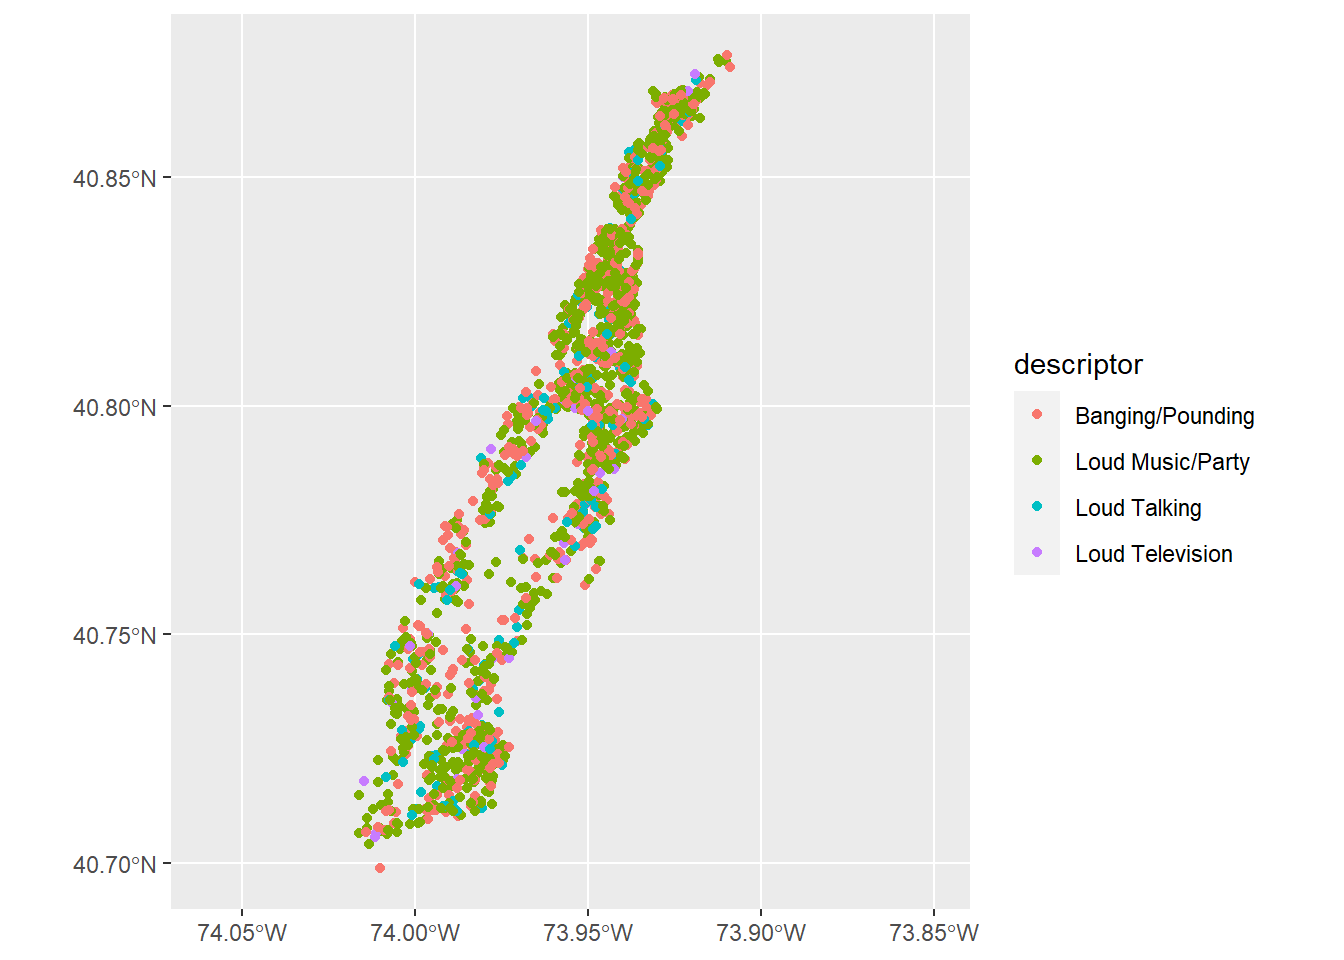
\includegraphics{R-spatial_files/figure-latex/ggplotQuickPlotSF-1.pdf}

\begin{Shaded}
\begin{Highlighting}[]
\NormalTok{man\_day\_noise\_sf }\OtherTok{\textless{}{-}}\NormalTok{ manhattan\_noise\_sf  }\SpecialCharTok{\%\textgreater{}\%} 
\NormalTok{         dplyr}\SpecialCharTok{::}\FunctionTok{filter}\NormalTok{(}\FunctionTok{day}\NormalTok{(datetime) }\SpecialCharTok{==} \DecValTok{19} \SpecialCharTok{\&} \FunctionTok{month}\NormalTok{(datetime) }\SpecialCharTok{==} \DecValTok{4} \SpecialCharTok{\&} \FunctionTok{year}\NormalTok{(datetime) }\SpecialCharTok{\textgreater{}} \DecValTok{2019}\NormalTok{); }

\FunctionTok{ggplot}\NormalTok{(}\AttributeTok{data =}\NormalTok{ man\_day\_noise\_sf) }\SpecialCharTok{+}
  \FunctionTok{geom\_sf}\NormalTok{(}\FunctionTok{aes}\NormalTok{(}\AttributeTok{color=}\NormalTok{descriptor)) }\SpecialCharTok{+}
  \FunctionTok{coord\_sf}\NormalTok{(}\AttributeTok{xlim =}  \FunctionTok{c}\NormalTok{(}\SpecialCharTok{{-}}\FloatTok{74.06}\NormalTok{, }\SpecialCharTok{{-}}\FloatTok{73.85}\NormalTok{), }\AttributeTok{crs =}\NormalTok{ sf}\SpecialCharTok{::}\FunctionTok{st\_crs}\NormalTok{(}\DecValTok{2831}\NormalTok{), }\AttributeTok{default\_crs =}\NormalTok{ sf}\SpecialCharTok{::}\FunctionTok{st\_crs}\NormalTok{(}\DecValTok{4326}\NormalTok{)) }\SpecialCharTok{+}
  \FunctionTok{labs}\NormalTok{(}\AttributeTok{title =} \StringTok{"Residential Noise 311 Calls in Manhattan"}\NormalTok{, }\AttributeTok{subtitle =} \StringTok{\textquotesingle{}April 19, 2019\textquotesingle{}}\NormalTok{)}
\end{Highlighting}
\end{Shaded}

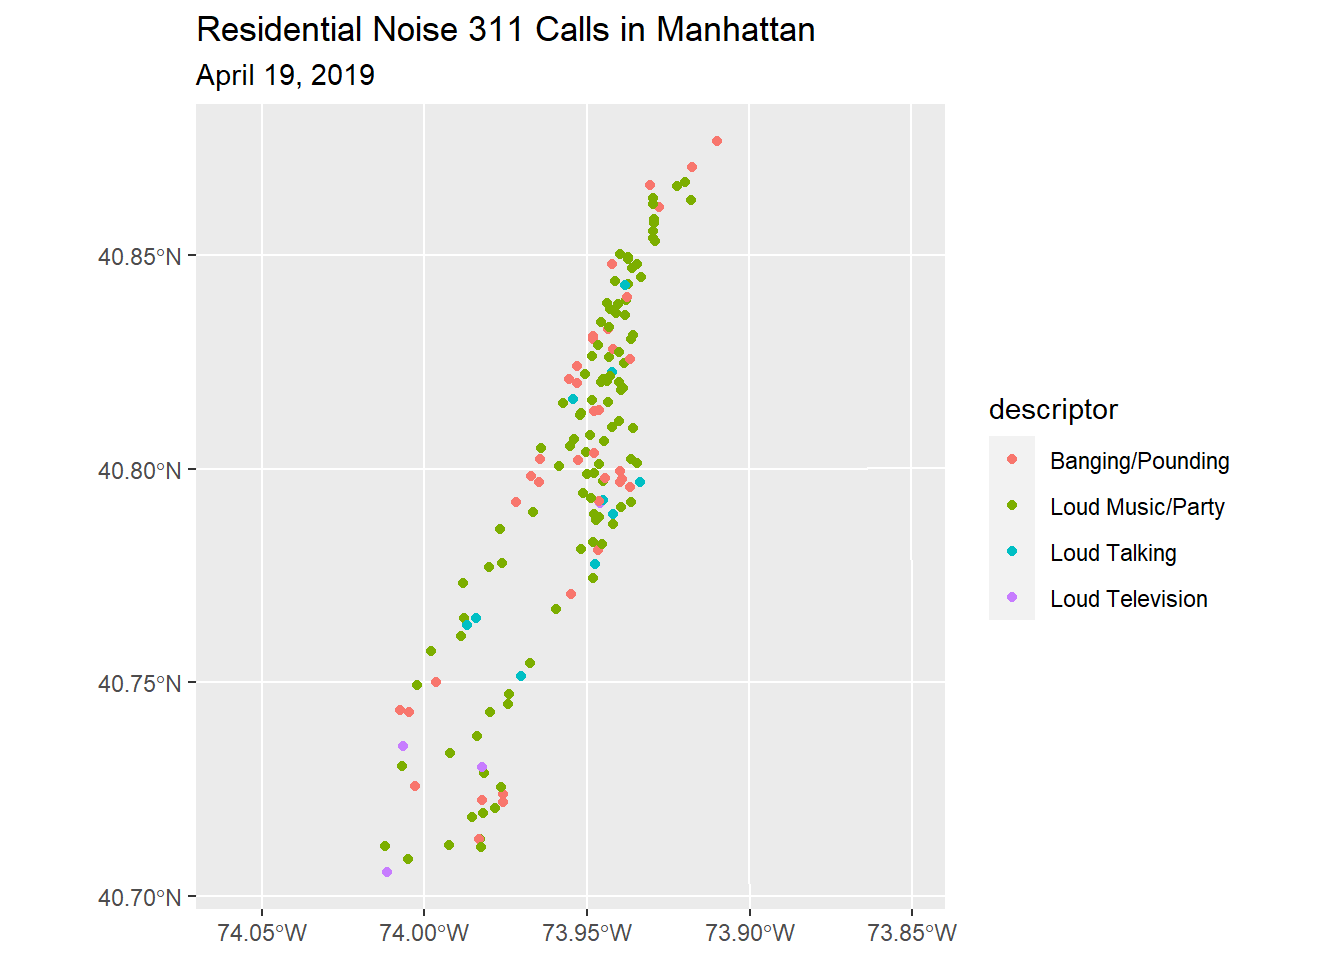
\includegraphics{R-spatial_files/figure-latex/ggplotQuickPlotSF-2.pdf}

Now, we use a base map to plot it again.

\begin{Shaded}
\begin{Highlighting}[]
\CommentTok{\# We can get a simple basemap. Adjust zoom with the map extent. }
\CommentTok{\# Higher zoom means more details but needs more time to load.}
\CommentTok{\# Start from small and increase to an appropriate level. Will learn more on this.}

\CommentTok{\# In most cases we can use the extent of the data to retrieve the basemap}
\NormalTok{manhattan\_noise\_sf }\SpecialCharTok{\%\textgreater{}\%} \FunctionTok{st\_bbox}\NormalTok{() }\SpecialCharTok{\%\textgreater{}\%} \FunctionTok{as.vector}\NormalTok{() }\SpecialCharTok{\%\textgreater{}\%}
\NormalTok{  ggmap}\SpecialCharTok{::}\FunctionTok{get\_stamenmap}\NormalTok{(}\AttributeTok{zoom =} \DecValTok{11}\NormalTok{, }\AttributeTok{messaging =} \ConstantTok{FALSE}\NormalTok{) }\OtherTok{{-}\textgreater{}}\NormalTok{ baseMap;}
\end{Highlighting}
\end{Shaded}

\begin{verbatim}
#> Source : http://tile.stamen.com/terrain/11/602/768.png
\end{verbatim}

\begin{verbatim}
#> Source : http://tile.stamen.com/terrain/11/603/768.png
\end{verbatim}

\begin{verbatim}
#> Source : http://tile.stamen.com/terrain/11/602/769.png
\end{verbatim}

\begin{verbatim}
#> Source : http://tile.stamen.com/terrain/11/603/769.png
\end{verbatim}

\begin{verbatim}
#> Source : http://tile.stamen.com/terrain/11/602/770.png
\end{verbatim}

\begin{verbatim}
#> Source : http://tile.stamen.com/terrain/11/603/770.png
\end{verbatim}

\begin{Shaded}
\begin{Highlighting}[]
\CommentTok{\# This is the ggplot style plotting. Again, will come back on this for more.}
\FunctionTok{ggmap}\NormalTok{(baseMap) }\SpecialCharTok{+}
  \FunctionTok{geom\_point}\NormalTok{(}\FunctionTok{aes}\NormalTok{(}\AttributeTok{x=}\NormalTok{X, }\AttributeTok{y=}\NormalTok{Y), }
             \AttributeTok{data =}\NormalTok{ man\_day\_noise\_sf }\SpecialCharTok{\%\textgreater{}\%} \FunctionTok{st\_coordinates}\NormalTok{() }\SpecialCharTok{\%\textgreater{}\%}\NormalTok{ tibble}\SpecialCharTok{::}\FunctionTok{as\_tibble}\NormalTok{(),}
             \AttributeTok{color =} \StringTok{\textquotesingle{}brown\textquotesingle{}}\NormalTok{,}
             \AttributeTok{size =} \DecValTok{1}\NormalTok{,}
             \AttributeTok{alpha =}\NormalTok{ .}\DecValTok{5}
\NormalTok{             )}
\end{Highlighting}
\end{Shaded}

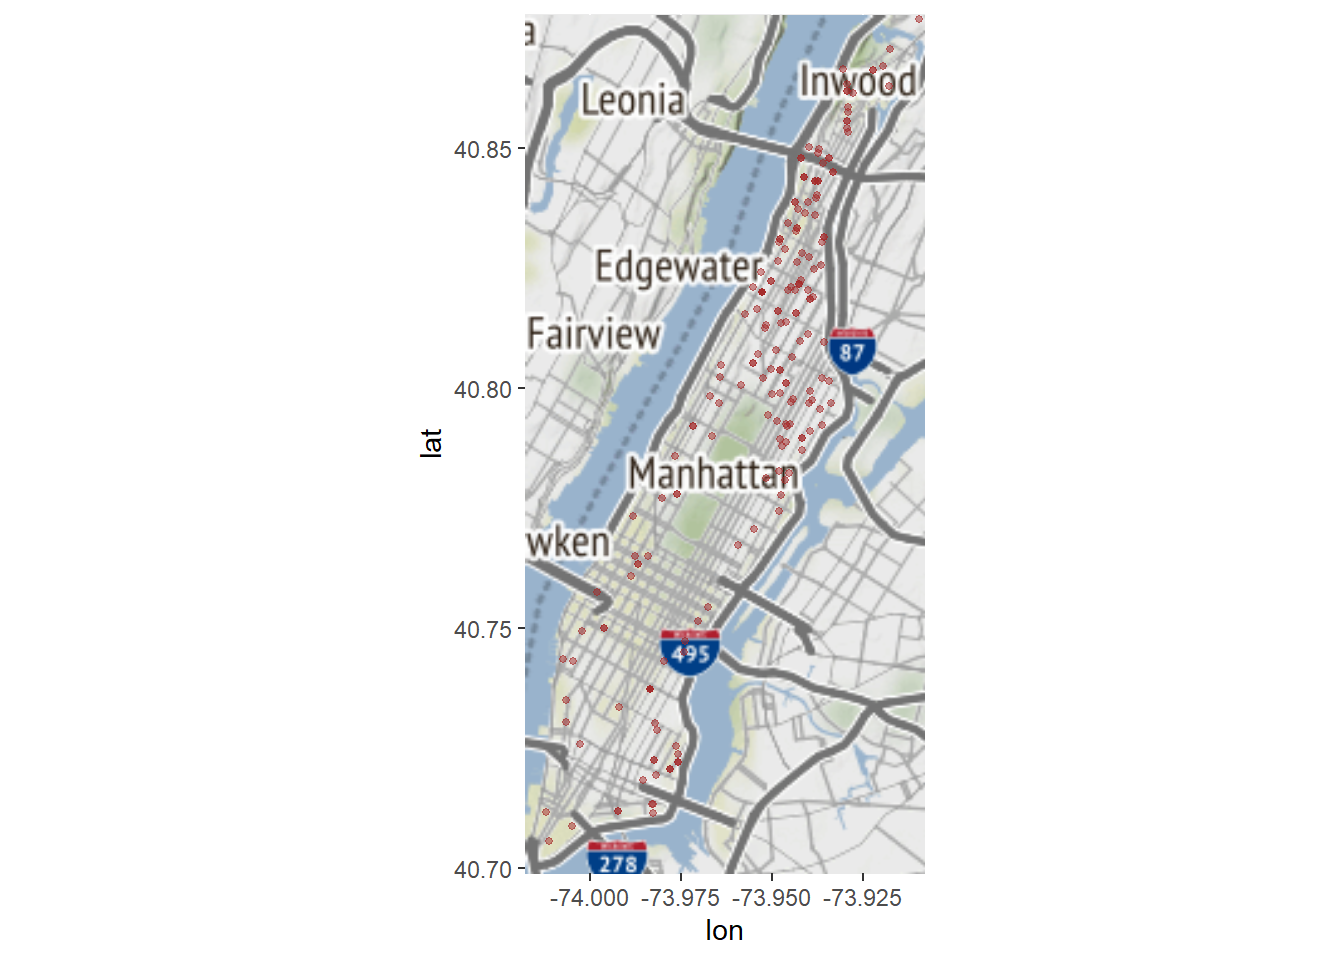
\includegraphics{R-spatial_files/figure-latex/ggmapQuickPlotSF-1.pdf}

\begin{Shaded}
\begin{Highlighting}[]
\CommentTok{\# but for the long shape of Manhattan, it might be better to manually choose the basemap}
\NormalTok{baseMapExt }\OtherTok{\textless{}{-}} \FunctionTok{c}\NormalTok{(}\SpecialCharTok{{-}}\FloatTok{74.06}\NormalTok{, }\FloatTok{40.691}\NormalTok{, }\SpecialCharTok{{-}}\FloatTok{73.85}\NormalTok{, }\FloatTok{40.879}\NormalTok{)}

\NormalTok{ggmap}\SpecialCharTok{::}\FunctionTok{get\_stamenmap}\NormalTok{(baseMapExt, }\AttributeTok{zoom =} \DecValTok{11}\NormalTok{, }\AttributeTok{messaging =} \ConstantTok{FALSE}\NormalTok{) }\OtherTok{{-}\textgreater{}}\NormalTok{ baseMap;}

\FunctionTok{ggmap}\NormalTok{(baseMap) }\SpecialCharTok{+}
  \FunctionTok{geom\_point}\NormalTok{(}\FunctionTok{aes}\NormalTok{(}\AttributeTok{x=}\NormalTok{X, }\AttributeTok{y=}\NormalTok{Y), }
             \AttributeTok{data =}\NormalTok{ man\_day\_noise\_sf }\SpecialCharTok{\%\textgreater{}\%} \FunctionTok{st\_coordinates}\NormalTok{() }\SpecialCharTok{\%\textgreater{}\%}\NormalTok{ tibble}\SpecialCharTok{::}\FunctionTok{as\_tibble}\NormalTok{(),}
             \AttributeTok{color =} \StringTok{\textquotesingle{}brown\textquotesingle{}}\NormalTok{,}
             \AttributeTok{size =} \DecValTok{1}\NormalTok{,}
             \AttributeTok{alpha =}\NormalTok{ .}\DecValTok{5}
\NormalTok{             ) }\SpecialCharTok{+} 
  \FunctionTok{labs}\NormalTok{(}\AttributeTok{title =} \StringTok{"Residential Noise 311 Calls in Manhattan"}\NormalTok{, }\AttributeTok{subtitle =} \StringTok{\textquotesingle{}April 19, 2019\textquotesingle{}}\NormalTok{)}
\end{Highlighting}
\end{Shaded}

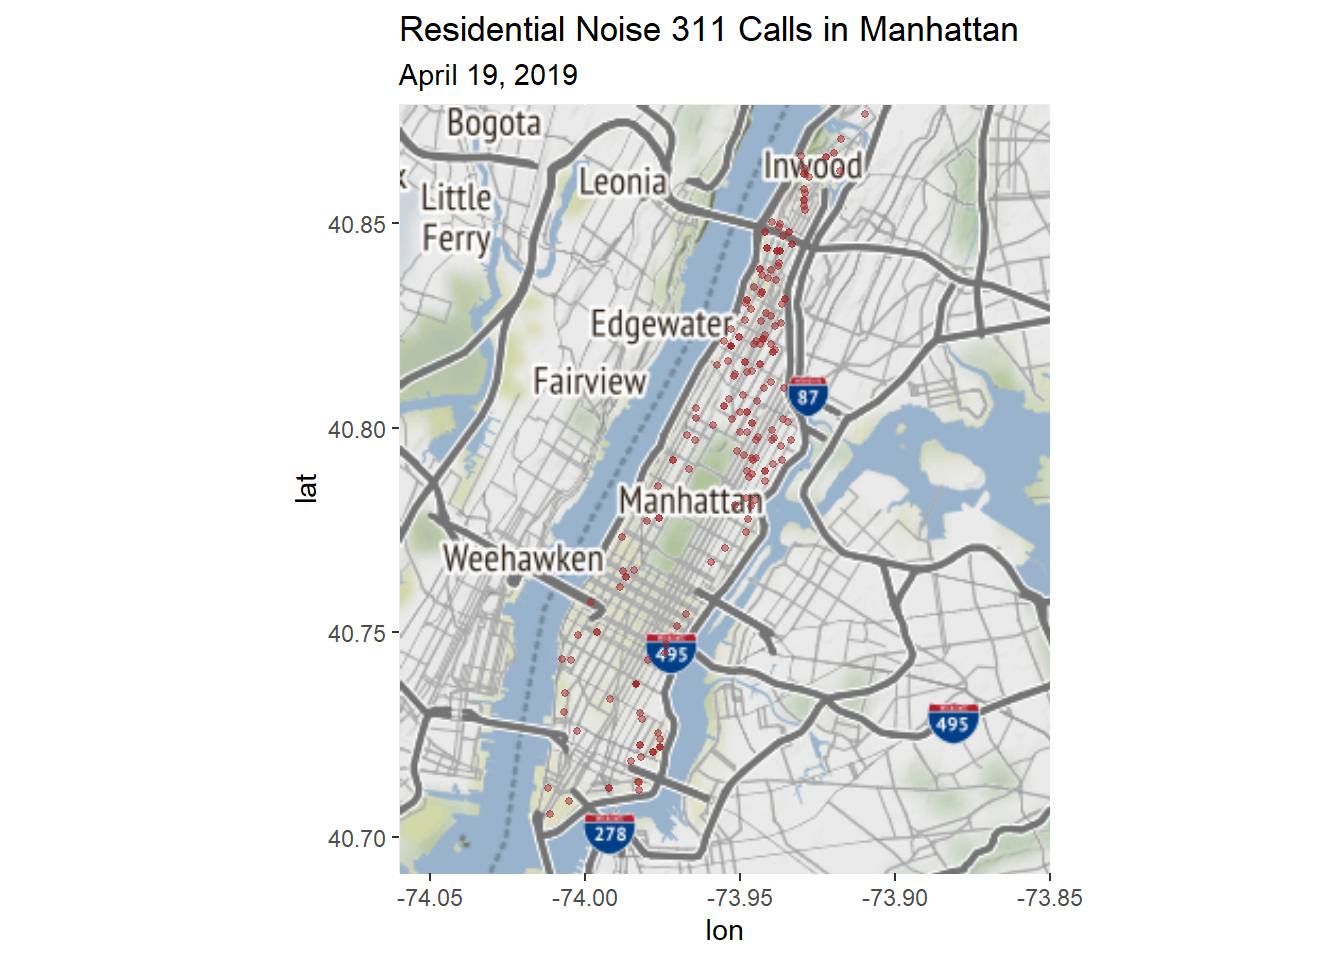
\includegraphics{R-spatial_files/figure-latex/ggmapQuickPlotSF-2.pdf}

Of course, \emph{mapview} comes in handy for creating simple interactive maps quickly.

\begin{Shaded}
\begin{Highlighting}[]
\FunctionTok{mapview}\NormalTok{(man\_day\_noise\_sf, }\AttributeTok{zcol=}\StringTok{\textquotesingle{}descriptor\textquotesingle{}}\NormalTok{, }\AttributeTok{layer.name=}\StringTok{\textquotesingle{}Manhattan Noise\textquotesingle{}}\NormalTok{)}
\end{Highlighting}
\end{Shaded}

\hypertarget{sp-and-sf-conversion}{%
\subsection{\texorpdfstring{\emph{sp} and \emph{sf} conversion}{sp and sf conversion}}\label{sp-and-sf-conversion}}

While \emph{sf} is the new standard, many classic packages are still using \emph{sp}. When needed, we can convert \emph{sf} objects to corresponding \emph{sp} objects or vice versa. Using sf::st\_as\_sf and sf::as\_Spatial, sp objects and sf objects can be converted to each other.

\begin{Shaded}
\begin{Highlighting}[]
\CommentTok{\# convert sf to sp}
\FunctionTok{class}\NormalTok{(manhattan\_noise\_sf)}
\NormalTok{manhattan\_noise\_sp\_ }\OtherTok{\textless{}{-}}\NormalTok{ sf}\SpecialCharTok{::}\FunctionTok{as\_Spatial}\NormalTok{(manhattan\_noise\_sf)}
\FunctionTok{class}\NormalTok{(manhattan\_noise\_sp\_)}

\CommentTok{\# Convert sp to sf}
\NormalTok{manhattan\_noise\_sf\_ }\OtherTok{\textless{}{-}}\NormalTok{ sf}\SpecialCharTok{::}\FunctionTok{st\_as\_sf}\NormalTok{(manhattan\_noise\_sp\_) }
\FunctionTok{class}\NormalTok{(manhattan\_noise\_sf\_)}
\end{Highlighting}
\end{Shaded}

\hypertarget{save-sf-objects}{%
\subsection{\texorpdfstring{Save \emph{sf} objects}{Save sf objects}}\label{save-sf-objects}}

We will save this object as a Shapefile on our hard drive for later use. (Note that by default \texttt{st\_write} checks if the file already exists, and if so it will not overwrite it. If you need to force it to overwrite use the option \texttt{delete\_layer\ =\ TRUE}.)

\begin{Shaded}
\begin{Highlighting}[]
\CommentTok{\# }
\FunctionTok{st\_write}\NormalTok{(manhattan\_noise\_sf, }\StringTok{"data/nyc"}\NormalTok{, }\StringTok{"ManhattanNoise"}\NormalTok{, }\AttributeTok{driver =} \StringTok{"ESRI Shapefile"}\NormalTok{)}
\CommentTok{\# to force the save: }
\FunctionTok{st\_write}\NormalTok{(manhattan\_noise\_sf, }\StringTok{"data/nyc/ManhattanNoise.shp"}\NormalTok{, }\AttributeTok{delete\_layer =} \ConstantTok{TRUE}\NormalTok{)}

\CommentTok{\# }
\FunctionTok{st\_write}\NormalTok{(man\_day\_noise\_sf, }\StringTok{\textquotesingle{}./data/nyc/manhattan\_day\_noise.shp\textquotesingle{}}\NormalTok{)}
\end{Highlighting}
\end{Shaded}

Shapefile is an outdated file format and has poor support for very large integers and datetime data types, for example. To completely save the data in R format, we can also directly save them as R data files. Of course, these files can only be used by R. Alternatively, we can use database-compatible format like GeoPackage, which is an OGC standard and increasingly popular, particular with QGIS.

\begin{Shaded}
\begin{Highlighting}[]
\CommentTok{\# Save data to RData file}
\FunctionTok{save}\NormalTok{(manhattan\_noise\_sf, man\_day\_noise\_sf, }
     \AttributeTok{file =} \StringTok{\textquotesingle{}./data/nyc/manhattan\_noise\_sf.RData\textquotesingle{}}\NormalTok{)}

\CommentTok{\# To get the data back into R}
\CommentTok{\# load(file=\textquotesingle{}./data/nyc/manhattan\_noise\_sf.RData\textquotesingle{})}

\CommentTok{\# Save data to a GeoPackage file/database}
\FunctionTok{st\_write}\NormalTok{(manhattan\_noise\_sf, }
         \AttributeTok{dsn =} \StringTok{\textquotesingle{}./data/nyc/man\_data.gpkg\textquotesingle{}}\NormalTok{, }
         \AttributeTok{layer=}\StringTok{\textquotesingle{}manhattan\_noise\textquotesingle{}}\NormalTok{,}
         \AttributeTok{delete\_layer =} \ConstantTok{TRUE}\NormalTok{)}

\FunctionTok{st\_write}\NormalTok{(man\_day\_noise\_sf,          }
         \AttributeTok{dsn =} \StringTok{\textquotesingle{}./data/nyc/man\_data.gpkg\textquotesingle{}}\NormalTok{, }
         \AttributeTok{layer=}\StringTok{\textquotesingle{}manhattan\_noise\_one\_day\textquotesingle{}}\NormalTok{,}
         \AttributeTok{delete\_layer =} \ConstantTok{TRUE}\NormalTok{)}

\CommentTok{\# Read in from geopackage}
\NormalTok{man\_one\_day\_noise }\OtherTok{\textless{}{-}} \FunctionTok{st\_read}\NormalTok{(}\AttributeTok{dsn =} \StringTok{\textquotesingle{}./data/nyc/man\_data.gpkg\textquotesingle{}}\NormalTok{, }
        \AttributeTok{layer=}\StringTok{\textquotesingle{}manhattan\_noise\_one\_day\textquotesingle{}}\NormalTok{)}
\end{Highlighting}
\end{Shaded}

\hypertarget{reprojecting-or-projection-transformation}{%
\section{Reprojecting or Projection Transformation}\label{reprojecting-or-projection-transformation}}

So far, all our data are using geographic coordinates in degrees. Sometimes, we may have to change the coordinates into a new Coordinate Reference System (CRS). For example, we retrieved census tracts data for the entire country, which are normally using geographic coordinates. For a local application at NYC, we need to reproject the data to a CRS that minimizes the distortion locally. With a local map projection, we can more accurately measures distances, areas, and angles.

Functions to \emph{transform}, or \emph{reproject} spatial objects typically take the following two arguments:

\begin{itemize}
\tightlist
\item
  the spatial object to transform
\item
  a CRS object with the new projection definition
\end{itemize}

You can transform

\begin{itemize}
\tightlist
\item
  a \emph{sf} object with \texttt{st\_transform()}\\
\item
  a \texttt{Spatial*} object with \texttt{spTransform()}\\
\item
  a \texttt{raster} object with \texttt{projectRaster()}
\end{itemize}

The perhaps trickiest part here is to determine the definition of the projection, which needs to be a character string in \href{http://trac.osgeo.org/proj/}{proj4} format or a number for SRID (spatial reference ID). You can \href{http://www.spatialreference.org}{look it up online}. For example for \href{http://spatialreference.org/ref/epsg/wgs-84-utm-zone-33n/}{UTM zone 33N (EPSG:32633)}, its SRID is 32633 and its proj4 string would be:

\href{http://spatialreference.org/ref/epsg/wgs-84-utm-zone-33n/proj4js/}{\texttt{+proj=utm\ +zone=33\ +ellps=WGS84\ +datum=WGS84\ +units=m\ +no\_defs}}

You can retrieve the CRS:

\begin{itemize}
\tightlist
\item
  from an \emph{sf} object with \texttt{st\_crs()}
\item
  from an existing \texttt{Spatial*} object with \texttt{proj4string()}
\item
  from a \texttt{raster} object with \texttt{crs()}
\end{itemize}

\hypertarget{transform-or-reproject-sf-objects}{%
\subsection{\texorpdfstring{Transform or reproject \textbf{\emph{sf}} objects}{Transform or reproject sf objects}}\label{transform-or-reproject-sf-objects}}

Let us check \texttt{nyc\_sf\_merged} object and reproject it to a local projection in State Plane Long Island, that is the map projection the NYC.

\begin{Shaded}
\begin{Highlighting}[]
\FunctionTok{st\_crs}\NormalTok{(man\_day\_noise\_sf)}
\end{Highlighting}
\end{Shaded}

\begin{verbatim}
#> Coordinate Reference System:
#>   User input: EPSG:4326 
#>   wkt:
#> GEOGCRS["WGS 84",
#>     DATUM["World Geodetic System 1984",
#>         ELLIPSOID["WGS 84",6378137,298.257223563,
#>             LENGTHUNIT["metre",1]]],
#>     PRIMEM["Greenwich",0,
#>         ANGLEUNIT["degree",0.0174532925199433]],
#>     CS[ellipsoidal,2],
#>         AXIS["geodetic latitude (Lat)",north,
#>             ORDER[1],
#>             ANGLEUNIT["degree",0.0174532925199433]],
#>         AXIS["geodetic longitude (Lon)",east,
#>             ORDER[2],
#>             ANGLEUNIT["degree",0.0174532925199433]],
#>     USAGE[
#>         SCOPE["Horizontal component of 3D system."],
#>         AREA["World."],
#>         BBOX[-90,-180,90,180]],
#>     ID["EPSG",4326]]
\end{verbatim}

\begin{Shaded}
\begin{Highlighting}[]
\CommentTok{\# then we transform/reproject it to SPCS Long Island, 2831}
\NormalTok{man\_day\_noise\_2831 }\OtherTok{\textless{}{-}} \FunctionTok{st\_transform}\NormalTok{(man\_day\_noise\_sf, }\DecValTok{2831}\NormalTok{)}

\FunctionTok{st\_crs}\NormalTok{(man\_day\_noise\_2831)}
\end{Highlighting}
\end{Shaded}

\begin{verbatim}
#> Coordinate Reference System:
#>   User input: EPSG:2831 
#>   wkt:
#> PROJCRS["NAD83(HARN) / New York Long Island",
#>     BASEGEOGCRS["NAD83(HARN)",
#>         DATUM["NAD83 (High Accuracy Reference Network)",
#>             ELLIPSOID["GRS 1980",6378137,298.257222101,
#>                 LENGTHUNIT["metre",1]]],
#>         PRIMEM["Greenwich",0,
#>             ANGLEUNIT["degree",0.0174532925199433]],
#>         ID["EPSG",4152]],
#>     CONVERSION["SPCS83 New York Long Island zone (meters)",
#>         METHOD["Lambert Conic Conformal (2SP)",
#>             ID["EPSG",9802]],
#>         PARAMETER["Latitude of false origin",40.1666666666667,
#>             ANGLEUNIT["degree",0.0174532925199433],
#>             ID["EPSG",8821]],
#>         PARAMETER["Longitude of false origin",-74,
#>             ANGLEUNIT["degree",0.0174532925199433],
#>             ID["EPSG",8822]],
#>         PARAMETER["Latitude of 1st standard parallel",41.0333333333333,
#>             ANGLEUNIT["degree",0.0174532925199433],
#>             ID["EPSG",8823]],
#>         PARAMETER["Latitude of 2nd standard parallel",40.6666666666667,
#>             ANGLEUNIT["degree",0.0174532925199433],
#>             ID["EPSG",8824]],
#>         PARAMETER["Easting at false origin",300000,
#>             LENGTHUNIT["metre",1],
#>             ID["EPSG",8826]],
#>         PARAMETER["Northing at false origin",0,
#>             LENGTHUNIT["metre",1],
#>             ID["EPSG",8827]]],
#>     CS[Cartesian,2],
#>         AXIS["easting (X)",east,
#>             ORDER[1],
#>             LENGTHUNIT["metre",1]],
#>         AXIS["northing (Y)",north,
#>             ORDER[2],
#>             LENGTHUNIT["metre",1]],
#>     USAGE[
#>         SCOPE["Engineering survey, topographic mapping."],
#>         AREA["United States (USA) - New York - counties of Bronx; Kings; Nassau; New York; Queens; Richmond; Suffolk."],
#>         BBOX[40.47,-74.26,41.3,-71.8]],
#>     ID["EPSG",2831]]
\end{verbatim}

We see that the CRS are different for the two. One is geographic coordinate systems (longitude, latitude) using WGS84 with a unit of decimal degree. And the other is New York State Plane Long Island with a unit of meter.

We can also see the proj4 strings of the two.

\begin{Shaded}
\begin{Highlighting}[]
\FunctionTok{st\_crs}\NormalTok{(man\_day\_noise\_sf)}\SpecialCharTok{$}\NormalTok{proj4string}
\FunctionTok{st\_crs}\NormalTok{(man\_day\_noise\_2831)}\SpecialCharTok{$}\NormalTok{proj4string}
\end{Highlighting}
\end{Shaded}

: we have \texttt{+proj=lcc...} and \texttt{+proj=longlat...}. LCC refers to Lambert Conic Conformal, which is a projected coordinate system with numeric units.

We can use the \texttt{st\_bbox()} method from the \emph{sf} package to compare the coordinates before and after reprojection and confirm that we actually have transformed them. \texttt{st\_bbox()} returns the \emph{min} and \emph{max} values of the two dimensions of a \emph{sf} spatial object.

\begin{Shaded}
\begin{Highlighting}[]
\NormalTok{sf}\SpecialCharTok{::}\FunctionTok{st\_bbox}\NormalTok{(man\_day\_noise\_sf) }\CommentTok{\# bounding box}
\end{Highlighting}
\end{Shaded}

\begin{verbatim}
#>      xmin      ymin      xmax      ymax 
#> -74.01208  40.70558 -73.90975  40.87673
\end{verbatim}

\begin{Shaded}
\begin{Highlighting}[]
\FunctionTok{st\_bbox}\NormalTok{(man\_day\_noise\_2831)}
\end{Highlighting}
\end{Shaded}

\begin{verbatim}
#>      xmin      ymin      xmax      ymax 
#> 298979.03  59842.73 307607.32  78853.14
\end{verbatim}

We can also visually compare the two map projections. While the differences are little bit hard to see, the locally projected map does stretch more along the horizontal direction.

\begin{Shaded}
\begin{Highlighting}[]
\CommentTok{\#par(mfrow=c(1,2))}
\FunctionTok{plot}\NormalTok{(man\_day\_noise\_sf }\SpecialCharTok{\%\textgreater{}\%} \FunctionTok{st\_geometry}\NormalTok{(),}\AttributeTok{pch=}\DecValTok{19}\NormalTok{,}\AttributeTok{col=}\StringTok{\textquotesingle{}blue\textquotesingle{}}\NormalTok{, }\AttributeTok{axes=}\ConstantTok{TRUE}\NormalTok{,}\AttributeTok{xaxs=}\StringTok{\textquotesingle{}r\textquotesingle{}}\NormalTok{, }\AttributeTok{graticule=}\FunctionTok{st\_crs}\NormalTok{(}\DecValTok{4326}\NormalTok{))}
\end{Highlighting}
\end{Shaded}

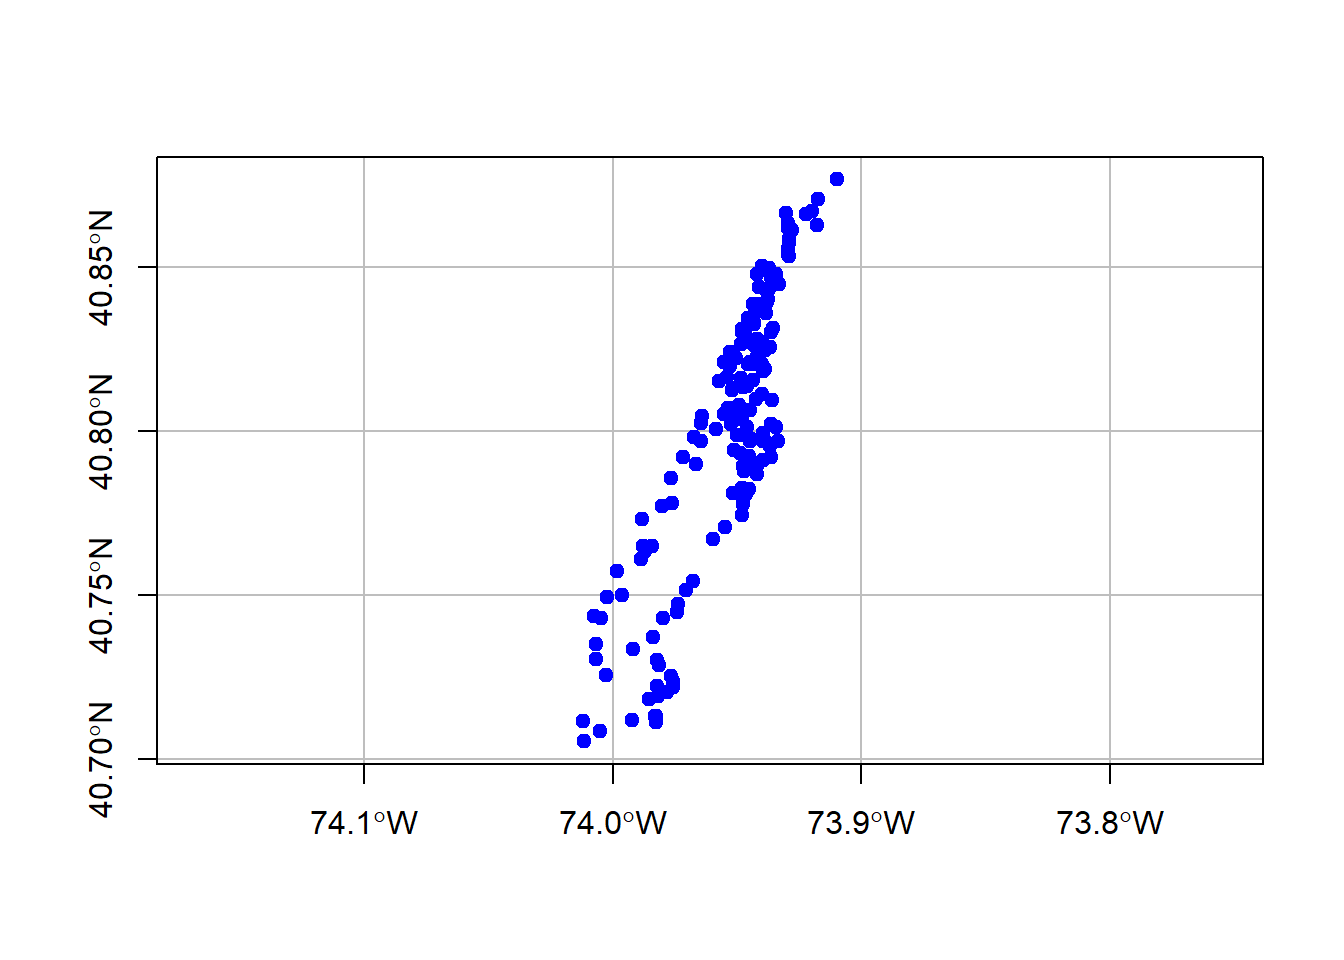
\includegraphics{R-spatial_files/figure-latex/visual-compare-1.pdf}

\begin{Shaded}
\begin{Highlighting}[]
\FunctionTok{plot}\NormalTok{(man\_day\_noise\_2831 }\SpecialCharTok{\%\textgreater{}\%} \FunctionTok{st\_geometry}\NormalTok{(),}\AttributeTok{pch=}\DecValTok{19}\NormalTok{,}\AttributeTok{col=}\StringTok{\textquotesingle{}red\textquotesingle{}}\NormalTok{, }\AttributeTok{axes=}\ConstantTok{TRUE}\NormalTok{,}\AttributeTok{xaxs=}\StringTok{\textquotesingle{}i\textquotesingle{}}\NormalTok{, }\AttributeTok{graticule=}\FunctionTok{st\_crs}\NormalTok{(}\DecValTok{2831}\NormalTok{))}
\end{Highlighting}
\end{Shaded}

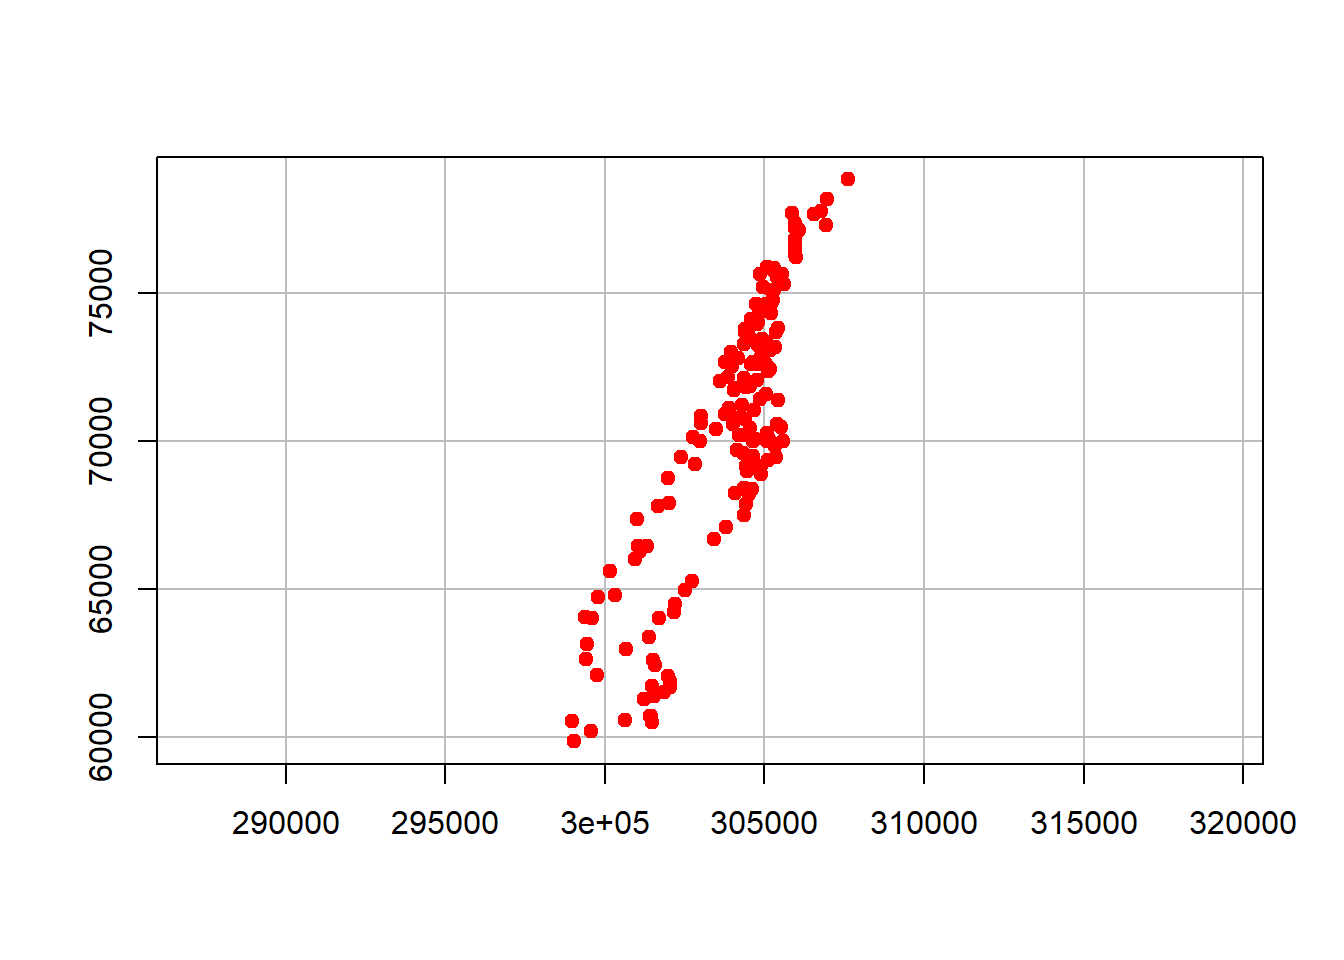
\includegraphics{R-spatial_files/figure-latex/visual-compare-2.pdf}

We will see later that using a local map projection with a unit of meter is necessary for spatial operations like buffer or other distance-based analyses.

\begin{quote}
\textbf{\emph{Set CRS and Reproject (transform)}}
\end{quote}

\begin{itemize}
\tightlist
\item
  Assigning a new CRS to a spatial object does not change its coordinates but the CRS determines how the software understand the coordinates. So, we must choose and set a CRS that is consistent with the coordinates. Otherwise, the coordinates will be misinterpreted.
\item
  Reprojecting spatial data with st\_transform and gTransform really changes the underlying coordinates, which we can see from the bbox values.\\
\item
  In either case, the CRS must be consistent with the coordinates. It is a good practice to check projected spatial data against a basemap or a correctly referenced map to verify its CRS.
\item
  \href{https://spatialreference.org/}{SpatialReference.org} is a very good source for CRS information.
\item
  Some commonly used reference systems

  \begin{itemize}
  \tightlist
  \item
    US 48 Contiguous States: Albers Equal Area (ESRI:102003), Lambert Conformal (ESRI:102004)
  \item
    New York State: UTM 18N (EPSG 3725, 3748, 26918)
  \item
    New York City: State Plane Long Island (EPSG 2263, 2831, 3627)
  \end{itemize}
\end{itemize}

\hypertarget{raster-data-in-r}{%
\section{Raster data in R}\label{raster-data-in-r}}

Raster files, as you might know, have a much more compact data structure than vectors. Because of their regular structure the coordinates do not need to be recorded for each pixel or cell in the rectangular extent. A raster is defined by:

\begin{itemize}
\tightlist
\item
  a CRS
\item
  coordinates of its origin
\item
  a distance or cell size in each direction
\item
  a dimension or numbers of cells in each direction
\item
  an array of cell values
\end{itemize}

Given this structure, coordinates for any cell can be computed and don't need to be stored.

The \texttt{raster} package\footnote{Note that \emph{sp} also allows to work with raster structures. The \texttt{GridTopology} class is the key element of raster representations. It contains: (a) the center coordinate pair of the south-west raster cell, (b) the two cell sizes in the metric of the coordinates, giving the step to successive centers, and (c) the numbers of cells for each dimension. There is also a \texttt{SpatialPixels} object which stores grid topology and coordinates of the actual points.} is a major extension of spatial data classes to access large rasters and in particular to process very large files. It includes object classes for \texttt{RasterLayer}, \texttt{RasterStacks}, and \texttt{RasterBricks}, functions for converting among these classes, and operators for computations on the raster data. Conversion from \emph{sp} type objects into \texttt{raster} type objects is possible.

If we wanted to do create a raster object from scratch we would do the following:

\begin{Shaded}
\begin{Highlighting}[]
\CommentTok{\# specify the RasterLayer with the following parameters:}
\CommentTok{\# {-} minimum x coordinate (left border)}
\CommentTok{\# {-} minimum y coordinate (bottom border)}
\CommentTok{\# {-} maximum x coordinate (right border)}
\CommentTok{\# {-} maximum y coordinate (top border)}
\CommentTok{\# {-} resolution (cell size) in each dimension}
\NormalTok{r }\OtherTok{\textless{}{-}} \FunctionTok{raster}\NormalTok{(}\AttributeTok{xmn=}\SpecialCharTok{{-}}\FloatTok{0.5}\NormalTok{, }\AttributeTok{ymn=}\SpecialCharTok{{-}}\FloatTok{0.5}\NormalTok{, }\AttributeTok{xmx=}\FloatTok{4.5}\NormalTok{, }\AttributeTok{ymx=}\FloatTok{4.5}\NormalTok{, }\AttributeTok{resolution=}\FunctionTok{c}\NormalTok{(}\DecValTok{1}\NormalTok{,}\DecValTok{1}\NormalTok{))}
\NormalTok{r}
\end{Highlighting}
\end{Shaded}

\begin{verbatim}
#> class      : RasterLayer 
#> dimensions : 5, 5, 25  (nrow, ncol, ncell)
#> resolution : 1, 1  (x, y)
#> extent     : -0.5, 4.5, -0.5, 4.5  (xmin, xmax, ymin, ymax)
#> crs        : +proj=longlat +datum=WGS84 +no_defs
\end{verbatim}

Note that this raster object \textbf{has a CRS defined!} If the crs argument is missing when creating the Raster object, the x coordinates are within -360 and 360 and the y coordinates are within -90 and 90, the WGS84 projection is used by default!

Good to know.

To add some values to the cells we could the following.

\begin{Shaded}
\begin{Highlighting}[]
\FunctionTok{class}\NormalTok{(r)}
\end{Highlighting}
\end{Shaded}

\begin{verbatim}
#> [1] "RasterLayer"
#> attr(,"package")
#> [1] "raster"
\end{verbatim}

\begin{Shaded}
\begin{Highlighting}[]
\NormalTok{r }\OtherTok{\textless{}{-}} \FunctionTok{setValues}\NormalTok{(r, }\FunctionTok{runif}\NormalTok{(}\DecValTok{25}\NormalTok{))}
\FunctionTok{class}\NormalTok{(r)}
\end{Highlighting}
\end{Shaded}

\begin{verbatim}
#> [1] "RasterLayer"
#> attr(,"package")
#> [1] "raster"
\end{verbatim}

\begin{Shaded}
\begin{Highlighting}[]
\FunctionTok{plot}\NormalTok{(r); }\FunctionTok{points}\NormalTok{(}\FunctionTok{coordinates}\NormalTok{(r), }\AttributeTok{pch=}\DecValTok{3}\NormalTok{)}
\end{Highlighting}
\end{Shaded}

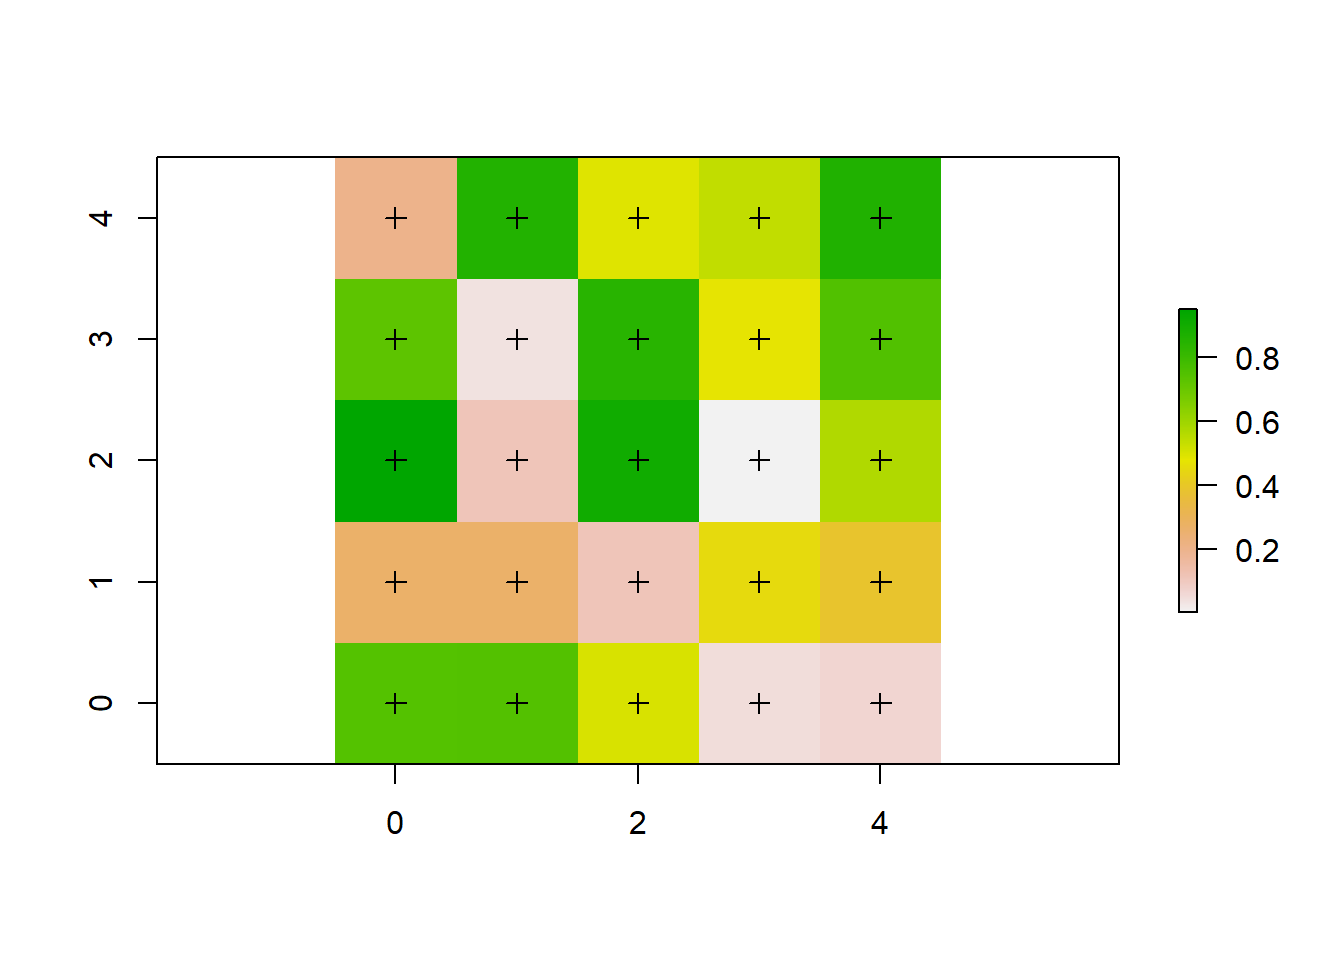
\includegraphics{R-spatial_files/figure-latex/unnamed-chunk-3-1.pdf}

(See the \href{https://cran.r-project.org/web/packages/rasterVis/index.html}{\texttt{rasterVis} package} for more advanced plotting of \texttt{Raster*} objects.)

RasterLayer objects can also be created from a matrix.

\begin{Shaded}
\begin{Highlighting}[]
\FunctionTok{class}\NormalTok{(volcano)}
\end{Highlighting}
\end{Shaded}

\begin{verbatim}
#> [1] "matrix" "array"
\end{verbatim}

\begin{Shaded}
\begin{Highlighting}[]
\NormalTok{volcano.r }\OtherTok{\textless{}{-}} \FunctionTok{raster}\NormalTok{(volcano)}
\FunctionTok{class}\NormalTok{(volcano.r)}
\end{Highlighting}
\end{Shaded}

\begin{verbatim}
#> [1] "RasterLayer"
#> attr(,"package")
#> [1] "raster"
\end{verbatim}

And to read in a raster file we can use the \texttt{raster()} function. This raster is generated as part of the \href{https://www.neonscience.org/field-sites/field-sites-map/HARV}{NEON Harvard Forest field site}.

\begin{Shaded}
\begin{Highlighting}[]
\FunctionTok{library}\NormalTok{(raster)}
\NormalTok{HARV }\OtherTok{\textless{}{-}} \FunctionTok{raster}\NormalTok{(}\StringTok{"data/HARV\_RGB\_Ortho.tif"}\NormalTok{)}
\end{Highlighting}
\end{Shaded}

Typing the name of the object will give us what's in there:

\begin{Shaded}
\begin{Highlighting}[]
\NormalTok{HARV}
\end{Highlighting}
\end{Shaded}

\begin{verbatim}
#> class      : RasterLayer 
#> band       : 1  (of  3  bands)
#> dimensions : 2317, 3073, 7120141  (nrow, ncol, ncell)
#> resolution : 0.25, 0.25  (x, y)
#> extent     : 731998.5, 732766.8, 4712956, 4713536  (xmin, xmax, ymin, ymax)
#> crs        : +proj=utm +zone=18 +datum=WGS84 +units=m +no_defs 
#> source     : HARV_RGB_Ortho.tif 
#> names      : HARV_RGB_Ortho 
#> values     : 0, 255  (min, max)
\end{verbatim}

We can plot it like this:

\begin{Shaded}
\begin{Highlighting}[]
\FunctionTok{plot}\NormalTok{(HARV)}
\end{Highlighting}
\end{Shaded}

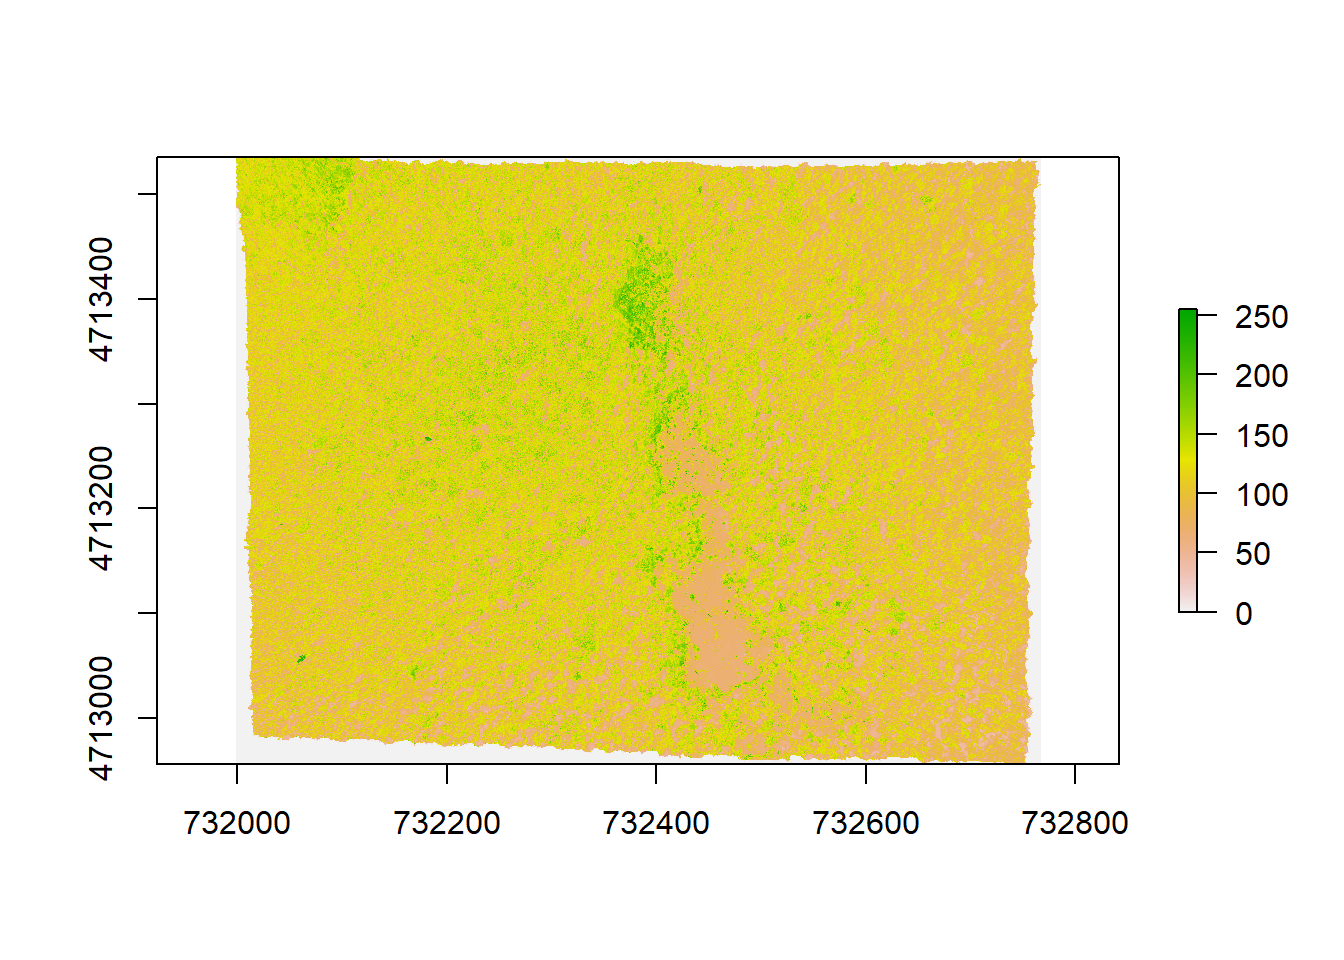
\includegraphics{R-spatial_files/figure-latex/plot-raster-1.pdf}

We can find out about the Coordinate Reference System with this:

\begin{Shaded}
\begin{Highlighting}[]
\FunctionTok{crs}\NormalTok{(HARV)}
\end{Highlighting}
\end{Shaded}

\begin{verbatim}
#> Coordinate Reference System:
#> Deprecated Proj.4 representation:
#>  +proj=utm +zone=18 +datum=WGS84 +units=m +no_defs 
#> WKT2 2019 representation:
#> PROJCRS["WGS 84 / UTM zone 18N",
#>     BASEGEOGCRS["WGS 84",
#>         DATUM["World Geodetic System 1984",
#>             ELLIPSOID["WGS 84",6378137,298.257223563,
#>                 LENGTHUNIT["metre",1]]],
#>         PRIMEM["Greenwich",0,
#>             ANGLEUNIT["degree",0.0174532925199433]],
#>         ID["EPSG",4326]],
#>     CONVERSION["UTM zone 18N",
#>         METHOD["Transverse Mercator",
#>             ID["EPSG",9807]],
#>         PARAMETER["Latitude of natural origin",0,
#>             ANGLEUNIT["degree",0.0174532925199433],
#>             ID["EPSG",8801]],
#>         PARAMETER["Longitude of natural origin",-75,
#>             ANGLEUNIT["degree",0.0174532925199433],
#>             ID["EPSG",8802]],
#>         PARAMETER["Scale factor at natural origin",0.9996,
#>             SCALEUNIT["unity",1],
#>             ID["EPSG",8805]],
#>         PARAMETER["False easting",500000,
#>             LENGTHUNIT["metre",1],
#>             ID["EPSG",8806]],
#>         PARAMETER["False northing",0,
#>             LENGTHUNIT["metre",1],
#>             ID["EPSG",8807]]],
#>     CS[Cartesian,2],
#>         AXIS["(E)",east,
#>             ORDER[1],
#>             LENGTHUNIT["metre",1]],
#>         AXIS["(N)",north,
#>             ORDER[2],
#>             LENGTHUNIT["metre",1]],
#>     USAGE[
#>         SCOPE["Engineering survey, topographic mapping."],
#>         AREA["Between 78°W and 72°W, northern hemisphere between equator and 84°N, onshore and offshore. Bahamas. Canada - Nunavut; Ontario; Quebec. Colombia. Cuba. Ecuador. Greenland. Haiti. Jamica. Panama. Turks and Caicos Islands. United States (USA). Venezuela."],
#>         BBOX[0,-78,84,-72]],
#>     ID["EPSG",32618]]
\end{verbatim}

See what you can do with such an object:

\begin{Shaded}
\begin{Highlighting}[]
\FunctionTok{methods}\NormalTok{(}\AttributeTok{class=}\FunctionTok{class}\NormalTok{(HARV))}
\end{Highlighting}
\end{Shaded}

\begin{verbatim}
#>   [1] !                     !=                    $                    
#>   [4] $<-                   %in%                  [                    
#>   [7] [[                    [[<-                  [<-                  
#>  [10] ==                    addLayer              adjacent             
#>  [13] aggregate             all.equal             area                 
#>  [16] Arith                 as.array              as.character         
#>  [19] as.data.frame         as.factor             as.integer           
#>  [22] as.list               as.logical            as.matrix            
#>  [25] as.raster             as.vector             asFactor             
#>  [28] atan2                 bandnr                barplot              
#>  [31] bbox                  boundaries            boxplot              
#>  [34] brick                 buffer                calc                 
#>  [37] cellFromRowCol        cellFromRowColCombine cellFromXY           
#>  [40] cellStats             clamp                 click                
#>  [43] clump                 coerce                colFromCell          
#>  [46] colFromX              colSums               Compare              
#>  [49] contour               coordinates           corLocal             
#>  [52] couldBeLonLat         cover                 crop                 
#>  [55] crosstab              crs<-                 cut                  
#>  [58] cv                    density               dim                  
#>  [61] dim<-                 direction             disaggregate         
#>  [64] distance              extend                extent               
#>  [67] extract               flip                  focal                
#>  [70] freq                  getValues             getValuesBlock       
#>  [73] getValuesFocal        gridDistance          hasValues            
#>  [76] head                  hist                  image                
#>  [79] init                  inMemory              interpolate          
#>  [82] intersect             is.factor             is.finite            
#>  [85] is.infinite           is.na                 is.nan               
#>  [88] isLonLat              KML                   labels               
#>  [91] layerize              length                levels               
#>  [94] levels<-              lines                 localFun             
#>  [97] log                   Logic                 mapView              
#> [100] mask                  match                 Math                 
#> [103] Math2                 maxValue              mean                 
#> [106] merge                 metadata              minValue             
#> [109] modal                 mosaic                names                
#> [112] names<-               ncell                 ncol                 
#> [115] ncol<-                nlayers               nrow                 
#> [118] nrow<-                origin                origin<-             
#> [121] overlay               persp                 plot                 
#> [124] predict               print                 proj4string          
#> [127] proj4string<-         quantile              raster               
#> [130] rasterize             ratify                readAll              
#> [133] readStart             readStop              reclassify           
#> [136] rectify               res                   res<-                
#> [139] resample              RGB                   rotate               
#> [142] rowColFromCell        rowFromCell           rowFromY             
#> [145] rowSums               sampleRandom          sampleRegular        
#> [148] sampleStratified      scale                 select               
#> [151] setMinMax             setValues             shift                
#> [154] show                  spplot                stack                
#> [157] stackSelect           stretch               subs                 
#> [160] subset                Summary               summary              
#> [163] t                     tail                  terrain              
#> [166] text                  trim                  unique               
#> [169] update                values                values<-             
#> [172] Which                 which.max             which.min            
#> [175] wkt                   writeRaster           writeStart           
#> [178] writeStop             writeValues           xFromCell            
#> [181] xFromCol              xmax                  xmax<-               
#> [184] xmin                  xmin<-                xres                 
#> [187] xyFromCell            yFromCell             yFromRow             
#> [190] ymax                  ymax<-                ymin                 
#> [193] ymin<-                yres                  zonal                
#> [196] zoom                 
#> see '?methods' for accessing help and source code
\end{verbatim}

We can explore the distribution of values contained within our raster using the hist() function which produces a histogram. Histograms are often useful in identifying outliers and bad data values in our raster data.

\begin{Shaded}
\begin{Highlighting}[]
\FunctionTok{hist}\NormalTok{(HARV)}
\end{Highlighting}
\end{Shaded}

\begin{verbatim}
#> Warning in .hist1(x, maxpixels = maxpixels, main = main, plot = plot, ...): 1%
#> of the raster cells were used. 100000 values used.
\end{verbatim}

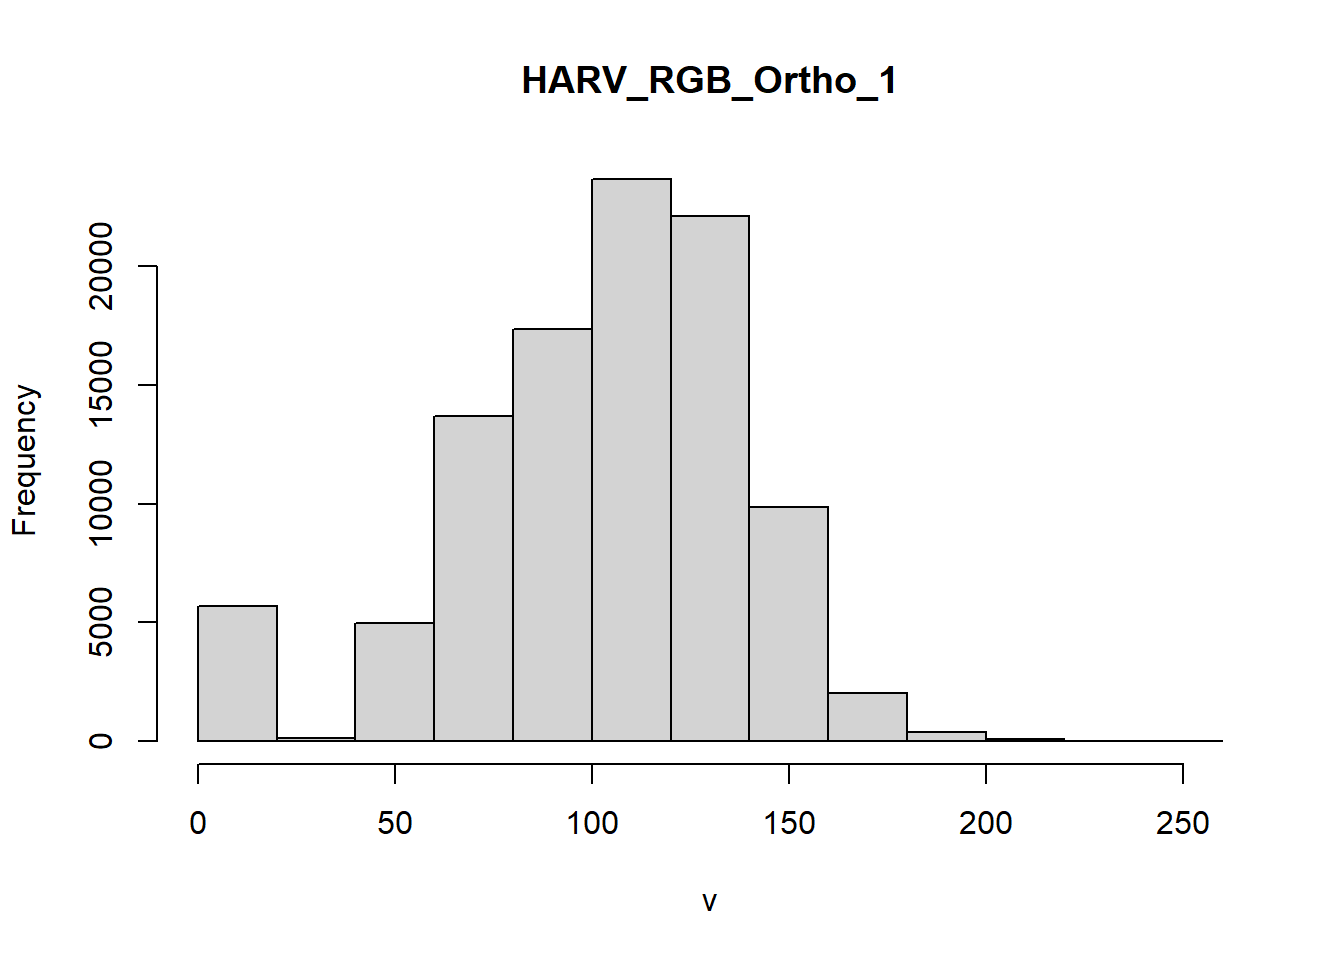
\includegraphics{R-spatial_files/figure-latex/n-hist-1.pdf}

Notice that a warning message is produced when R creates the histogram.

This warning is caused by the default maximum pixels value of 100,000 associated with the hist function. This maximum value is to ensure processing efficiency as our data become larger! We can force the \texttt{hist} function to use all cell values.

\begin{Shaded}
\begin{Highlighting}[]
\FunctionTok{ncell}\NormalTok{(HARV)}
\end{Highlighting}
\end{Shaded}

\begin{verbatim}
#> [1] 7120141
\end{verbatim}

\begin{Shaded}
\begin{Highlighting}[]
\FunctionTok{hist}\NormalTok{(HARV, }\AttributeTok{maxpixels =} \FunctionTok{ncell}\NormalTok{(HARV))}
\end{Highlighting}
\end{Shaded}

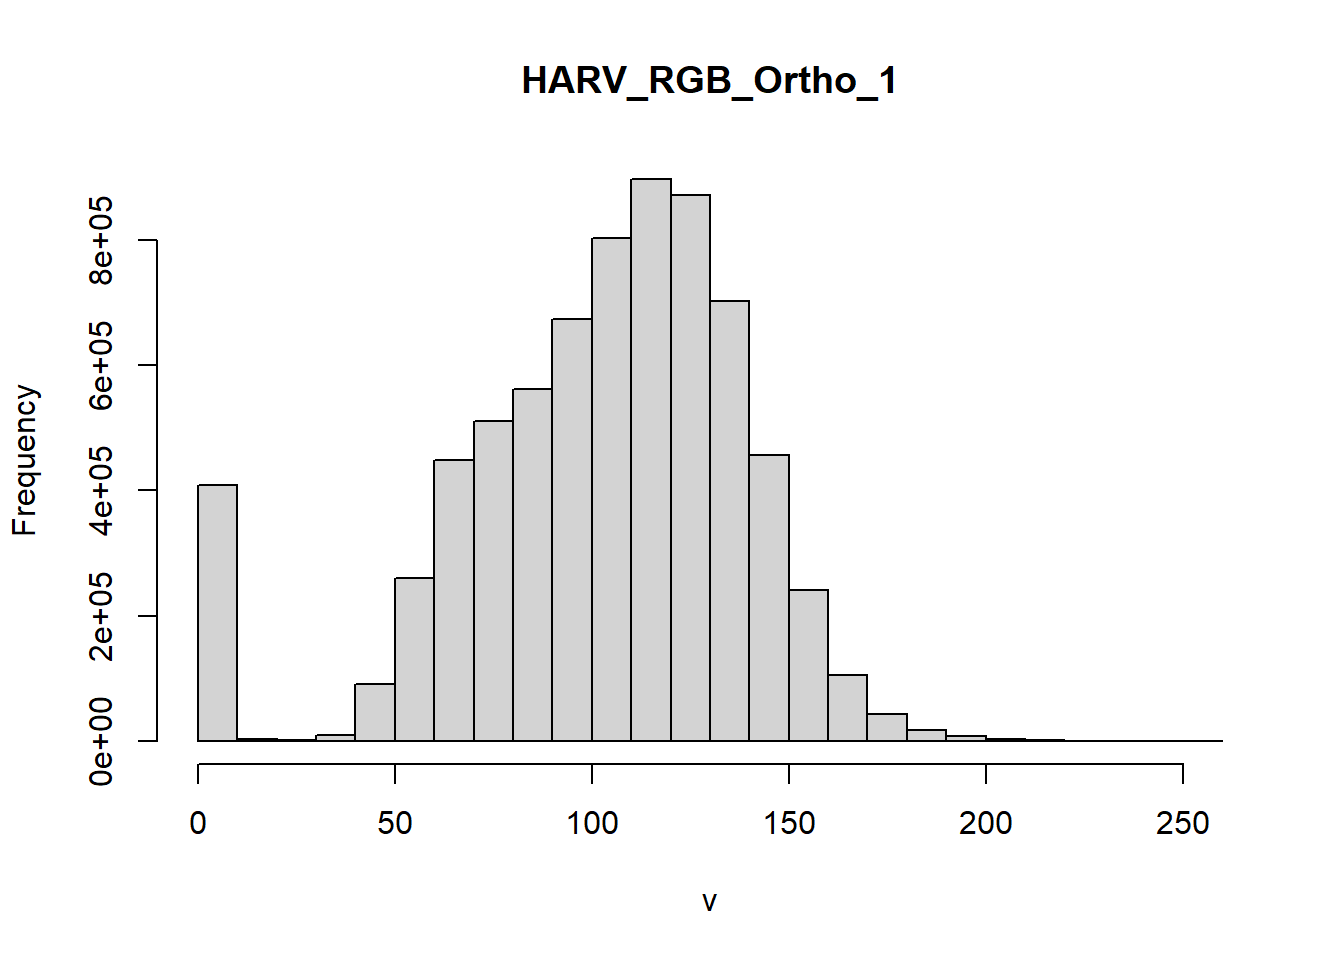
\includegraphics{R-spatial_files/figure-latex/n-hist-allvals-1.pdf}

At times it may be useful to explore raster metadata before loading them into R. This can be done with:

\begin{verbatim}
GDALinfo("path-to-raster-here") 
\end{verbatim}

A raster dataset can contain one or more bands. We can view the number of bands in a raster using the \texttt{nlayers()} function.

\begin{Shaded}
\begin{Highlighting}[]
\FunctionTok{nlayers}\NormalTok{(HARV)}
\end{Highlighting}
\end{Shaded}

\begin{verbatim}
#> [1] 1
\end{verbatim}

We can use the \texttt{raster()} function to import one single band from a \emph{single} \textbf{OR} from a \emph{multi-band} raster. For multi-band raster, we can specify which band we want to read in.

\begin{Shaded}
\begin{Highlighting}[]
\NormalTok{HARV\_Band2 }\OtherTok{\textless{}{-}} \FunctionTok{raster}\NormalTok{(}\StringTok{"data/HARV\_RGB\_Ortho.tif"}\NormalTok{, }\AttributeTok{band =} \DecValTok{2}\NormalTok{)}
\FunctionTok{plot}\NormalTok{(HARV\_Band2)}
\end{Highlighting}
\end{Shaded}

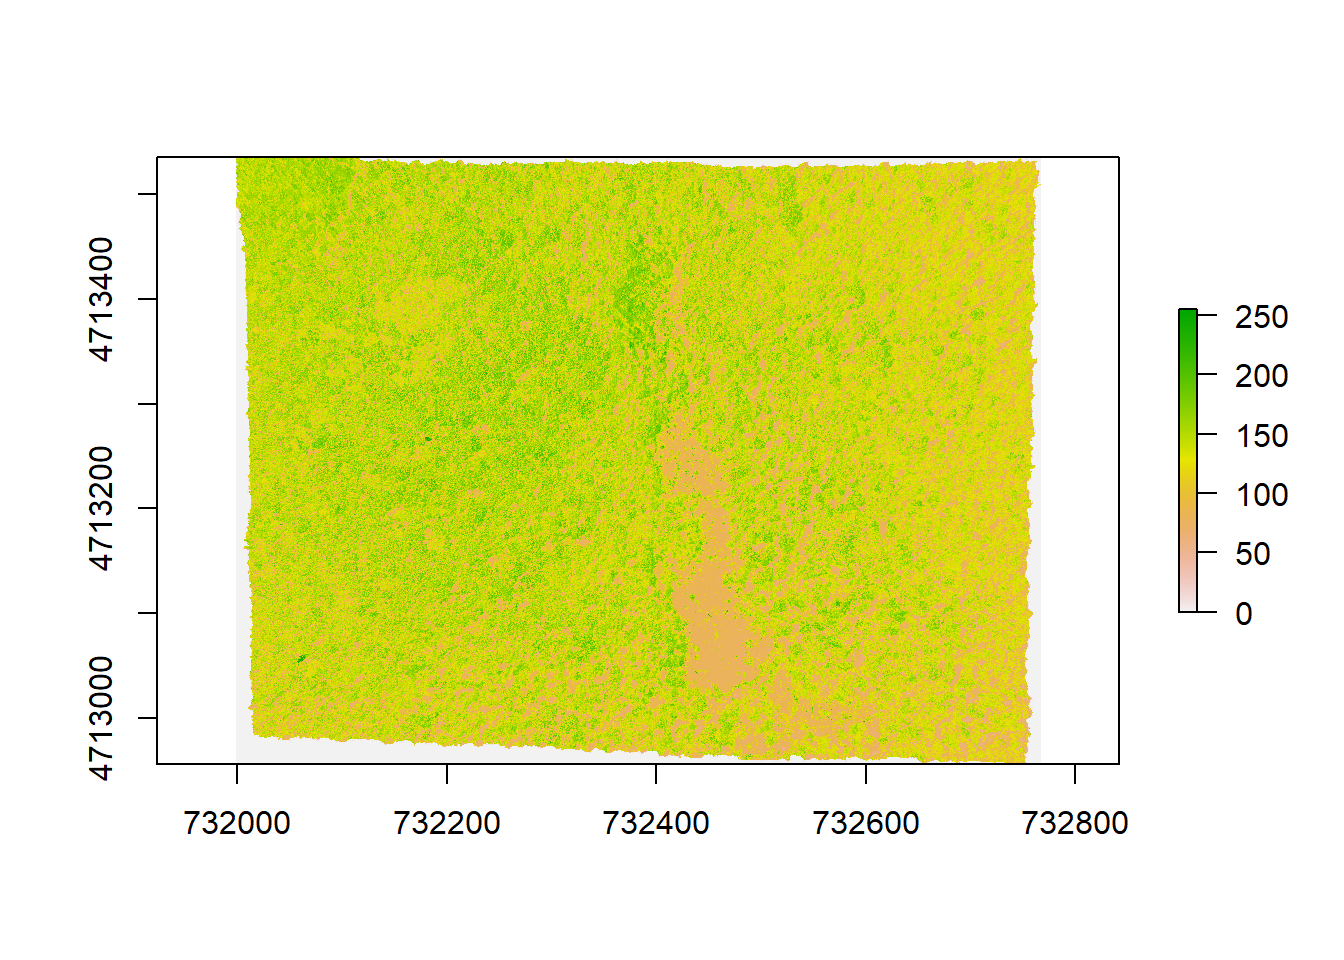
\includegraphics{R-spatial_files/figure-latex/one-multiband-1.pdf}

To bring in all bands of a multi-band raster, we use the \texttt{stack()} function.

\begin{Shaded}
\begin{Highlighting}[]
\NormalTok{HARV\_stack }\OtherTok{\textless{}{-}} \FunctionTok{stack}\NormalTok{(}\StringTok{"data/HARV\_RGB\_Ortho.tif"}\NormalTok{)}

\CommentTok{\# how many layers?}
\FunctionTok{nlayers}\NormalTok{(HARV\_stack)}
\end{Highlighting}
\end{Shaded}

\begin{verbatim}
#> [1] 3
\end{verbatim}

\begin{Shaded}
\begin{Highlighting}[]
\CommentTok{\# view attributes of stack object}
\NormalTok{HARV\_stack}
\end{Highlighting}
\end{Shaded}

\begin{verbatim}
#> class      : RasterStack 
#> dimensions : 2317, 3073, 7120141, 3  (nrow, ncol, ncell, nlayers)
#> resolution : 0.25, 0.25  (x, y)
#> extent     : 731998.5, 732766.8, 4712956, 4713536  (xmin, xmax, ymin, ymax)
#> crs        : +proj=utm +zone=18 +datum=WGS84 +units=m +no_defs 
#> names      : HARV_RGB_Ortho.1, HARV_RGB_Ortho.2, HARV_RGB_Ortho.3 
#> min values :                0,                0,                0 
#> max values :              255,              255,              255
\end{verbatim}

What happens when we plot?

\begin{Shaded}
\begin{Highlighting}[]
\FunctionTok{plot}\NormalTok{(HARV\_stack)}
\end{Highlighting}
\end{Shaded}

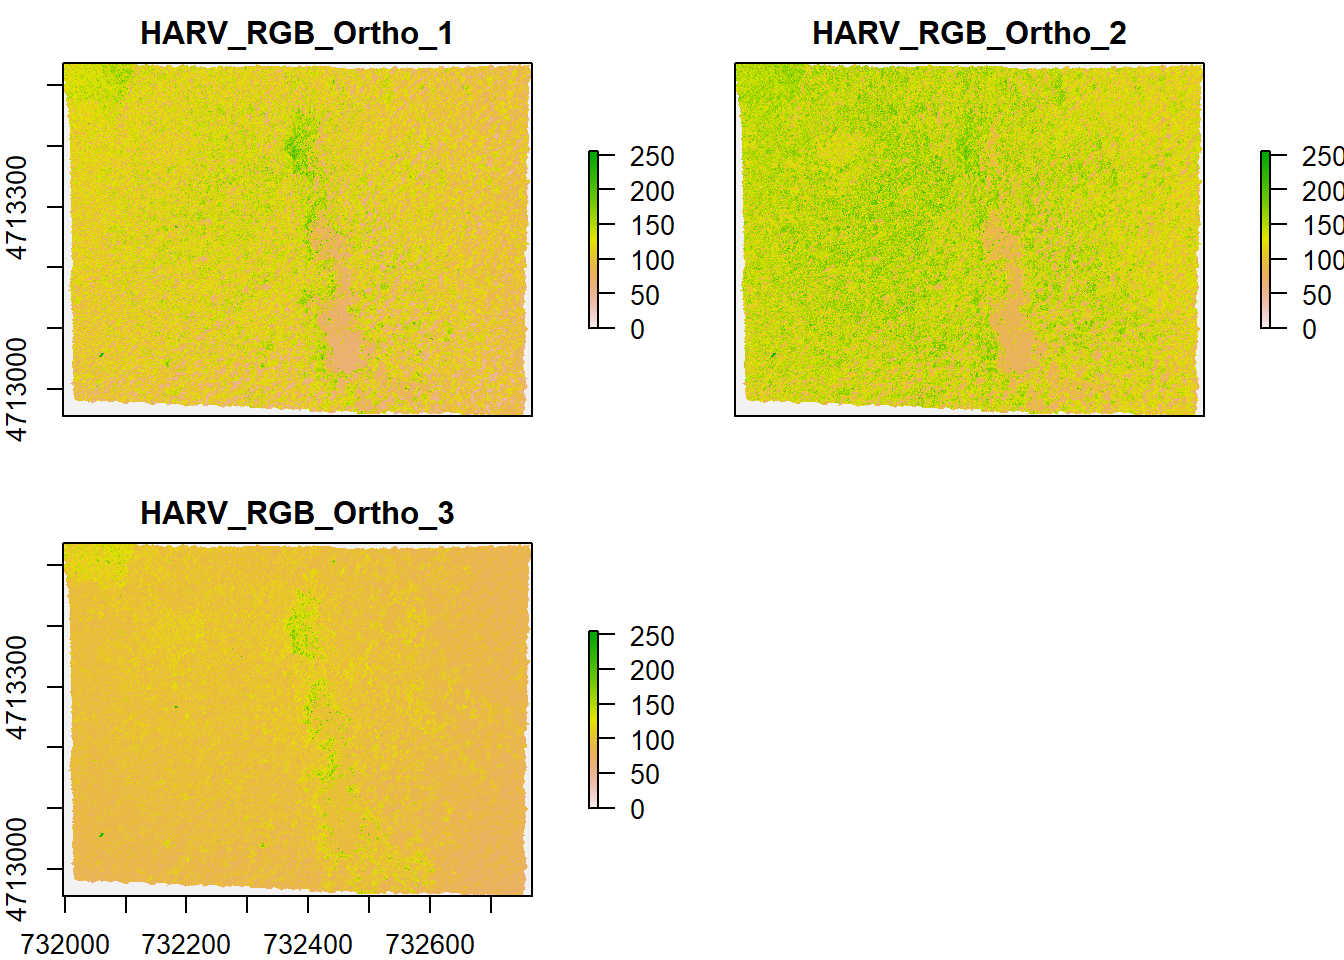
\includegraphics{R-spatial_files/figure-latex/stack-plot-1.pdf}

If we know that it is an RGB multiband raster we can plot them all in one

\begin{Shaded}
\begin{Highlighting}[]
\FunctionTok{plotRGB}\NormalTok{(HARV\_stack)}
\end{Highlighting}
\end{Shaded}

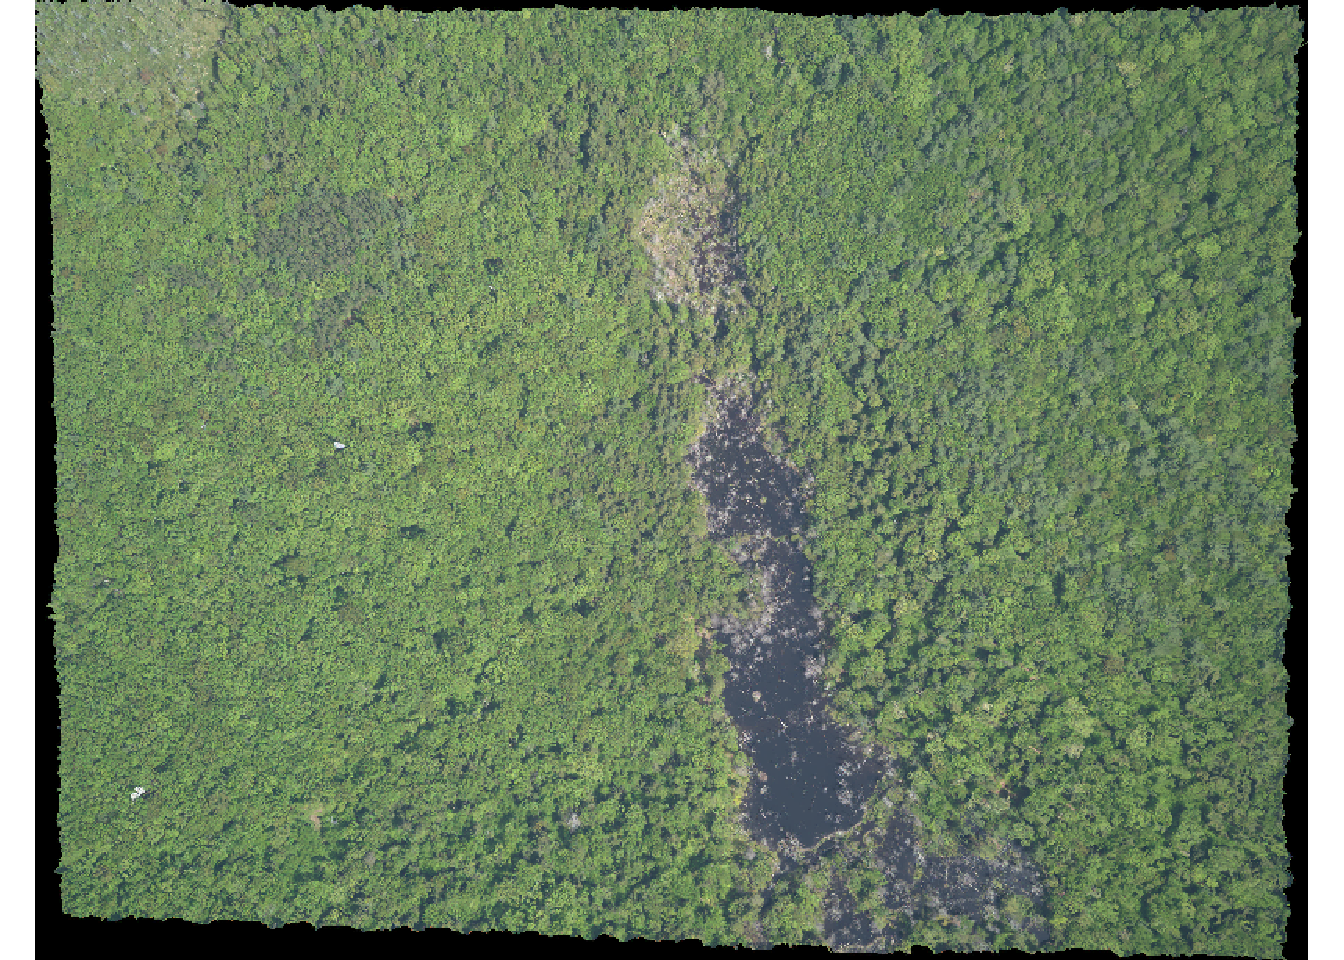
\includegraphics{R-spatial_files/figure-latex/stack-rgb-plot-1.pdf}

\hypertarget{rasterstack-vs-rasterbrick}{%
\subsection{RasterStack vs RasterBrick}\label{rasterstack-vs-rasterbrick}}

The R \texttt{RasterStack} and \texttt{RasterBrick} object types can both store multiple bands. However, how they store each band is different. The bands in a \texttt{RasterStack} are stored as links to raster data that is located somewhere on our computer. A \texttt{RasterBrick} contains all of the objects stored within the actual R object. Since in the \texttt{RasterBrick}, all of the bands are stored within the actual object its object size is much larger than the \texttt{RasterStack} object.

In most cases, we can work with a \texttt{RasterBrick} in the same way we might work with a \texttt{RasterStack}. However, a \texttt{RasterBrick} is often more efficient and faster to process - which is important when working with larger files.

We can turn a \texttt{RasterStack} into a \texttt{RasterBrick} in R by using \texttt{brick(StackName)}. Use the \texttt{object.size()} function to compare stack and brick R objects.

\begin{Shaded}
\begin{Highlighting}[]
\FunctionTok{object.size}\NormalTok{(HARV\_stack)}
\end{Highlighting}
\end{Shaded}

\begin{verbatim}
#> 51224 bytes
\end{verbatim}

\begin{Shaded}
\begin{Highlighting}[]
\NormalTok{HARV\_brick }\OtherTok{\textless{}{-}} \FunctionTok{brick}\NormalTok{(HARV\_stack)}
\FunctionTok{object.size}\NormalTok{(HARV\_brick)}
\end{Highlighting}
\end{Shaded}

\begin{verbatim}
#> 170898912 bytes
\end{verbatim}

Going back to the \emph{sp} package, a simple grid can be built like this:

\begin{Shaded}
\begin{Highlighting}[]
\CommentTok{\# specify the grid topology with the following parameters:}
\CommentTok{\# {-} the smallest coordinates for each dimension, here: 0,0}
\CommentTok{\# {-} cell size in each dimension, here: 1,1 }
\CommentTok{\# {-} number of cells in each dimension, here: 5,5}
\NormalTok{gtopo }\OtherTok{\textless{}{-}} \FunctionTok{GridTopology}\NormalTok{(}\FunctionTok{c}\NormalTok{(}\DecValTok{0}\NormalTok{,}\DecValTok{0}\NormalTok{), }\FunctionTok{c}\NormalTok{(}\DecValTok{1}\NormalTok{,}\DecValTok{1}\NormalTok{), }\FunctionTok{c}\NormalTok{(}\DecValTok{5}\NormalTok{,}\DecValTok{5}\NormalTok{)) }\CommentTok{\# create the grid}
\NormalTok{datafr }\OtherTok{\textless{}{-}} \FunctionTok{data.frame}\NormalTok{(}\FunctionTok{runif}\NormalTok{(}\DecValTok{25}\NormalTok{)) }\CommentTok{\# make up some data}
\NormalTok{SpGdf }\OtherTok{\textless{}{-}} \FunctionTok{SpatialGridDataFrame}\NormalTok{(gtopo, datafr) }\CommentTok{\# create the grid data frame}
\FunctionTok{summary}\NormalTok{(SpGdf)}
\end{Highlighting}
\end{Shaded}

\begin{verbatim}
#> Object of class SpatialGridDataFrame
#> Coordinates:
#>       min max
#> [1,] -0.5 4.5
#> [2,] -0.5 4.5
#> Is projected: NA 
#> proj4string : [NA]
#> Grid attributes:
#>   cellcentre.offset cellsize cells.dim
#> 1                 0        1         5
#> 2                 0        1         5
#> Data attributes:
#>    runif.25.     
#>  Min.   :0.0982  
#>  1st Qu.:0.4461  
#>  Median :0.6745  
#>  Mean   :0.6100  
#>  3rd Qu.:0.7878  
#>  Max.   :0.9915
\end{verbatim}

\hypertarget{lab-assignment}{%
\section{Lab Assignment}\label{lab-assignment}}

For the R-Spatial Section labs, we will do some spatial data visualization on COVID-19 in NYC. More specifically, we will explore the distribution of confirmed cases across the city and their relationships with some demographic variables and essential services related to retail food stores and public health services.

The first lab is rather simple and straightforward but will be the foundation for the next steps.

Tasks for the first lab are:

\begin{enumerate}
\def\labelenumi{\arabic{enumi}.}
\tightlist
\item
  Set up a R project for the R-Spatial section.
\item
  Read the NYC postal areas in Shapefiles into \emph{sf} objects. As NYC DOH publishes COVID-19 data by zip code, we will utilize the postal area data later.
\item
  Read and process the NYC public health services spreadsheet data. Create \emph{sf} objects from geographic coordinates.
\item
  Read and process the NYS retail food stores data. Create \emph{sf} objects from geographic coordinates for NYC.
\item
  Use simple mapping method, either based on \texttt{ggmap}+\texttt{ggplot} or \emph{mapview}, with a basemap to verify the above datasets in terms of their geometry locations.
\item
  Save the three \emph{sf} objects in a RData file or in a single GeoPackage file/database.
\end{enumerate}

The assignment and data are available on Blackboard. The data are also available for download at the Dropbox site.

\hypertarget{spatialops}{%
\chapter{Spatial data manipulation in R}\label{spatialops}}

\begin{quote}
Learning Objectives

\begin{itemize}
\tightlist
\item
  Join attribute data to a polygon vector file
\item
  Select data using attribute and spatial relationships
\item
  Reproject spatial data
\item
  Aggregate spatial data using spatial relationships
\end{itemize}
\end{quote}

\begin{center}\rule{0.5\linewidth}{0.5pt}\end{center}

There are a wide variety of spatial, topological, and attribute data operations we can perform with R. \href{https://geocompr.robinlovelace.net}{Lovelace et al's recent publication}\footnote{Lovelace, R., Nowosad, J., \& Muenchow, J. (2019). Geocomputation with R. CRC Press.} goes into great depth about this and is highly recommended.

In this section we will look at just a few examples for libraries and functions that allow us to process spatial data in R and perform some commonly used operations.

\hypertarget{attribute-join}{%
\section{Attribute Join}\label{attribute-join}}

An attribute join on vector data brings tabular data into a geographic context. It refers to the process of joining data in tabular format to data in a format that holds the geometries (polygon, line, or point)\footnote{Per the \href{http://www.esri.com/library/whitepapers/pdfs/shapefile.pdf}{ESRI specification} a Shapefile must have an attribute table, so when we read it into R with the \texttt{readOGR} command from the \emph{sp} package it automatically becomes a \texttt{Spatial*Dataframe} and the attribute table becomes the data.frame.}.

If you have done attribute joins of shapefiles in GIS software like \emph{ArcGIS} or \emph{QGIS} you know that you need a \textbf{unique identifier} in both the attribute table of the Shapefile and the table to be joined.

First we will load the CSV table \texttt{nyc\_census\_tracts\_pophu.csv} into a tibble dataframe in R tidyverse and name it \texttt{nyc\_pophu} for population and housing unit information.

\begin{Shaded}
\begin{Highlighting}[]
\NormalTok{nyc\_pophu }\OtherTok{\textless{}{-}}\NormalTok{ readr}\SpecialCharTok{::}\FunctionTok{read\_csv}\NormalTok{(}\StringTok{"data/nyc/nyc\_census\_tracts\_pophu.csv"}\NormalTok{, }\AttributeTok{lazy =} \ConstantTok{FALSE}\NormalTok{)}
\FunctionTok{str}\NormalTok{(nyc\_pophu)}
\end{Highlighting}
\end{Shaded}

\begin{verbatim}
#> spec_tbl_df [2,164 x 12] (S3: spec_tbl_df/tbl_df/tbl/data.frame)
#>  $ GEOID10   : num [1:2164] 3.6e+10 3.6e+10 3.6e+10 3.6e+10 3.6e+10 ...
#>  $ STATEFP   : num [1:2164] 36 36 36 36 36 36 36 36 36 36 ...
#>  $ COUNTYFP  : chr [1:2164] "005" "005" "005" "005" ...
#>  $ TRACTCE   : chr [1:2164] "002300" "002701" "004100" "004800" ...
#>  $ AFFGEOID  : chr [1:2164] "1400000US36005002300" "1400000US36005002701" "1400000US36005004100" "1400000US36005004800" ...
#>  $ POPULATION: num [1:2164] 4774 3016 6476 3999 7421 ...
#>  $ MEDAGE    : num [1:2164] 29 29 23 30 28 28 29 44 38 39 ...
#>  $ MEDHHINC  : num [1:2164] 14479 20153 18636 30301 21016 ...
#>  $ MEDHOUSING: num [1:2164] 406 627 655 1066 753 ...
#>  $ PCPREWAR  : num [1:2164] 26.8 40.6 31.3 51.1 37.3 55.5 52 19.7 18.9 18.7 ...
#>  $ MEDYRBUILT: num [1:2164] 1957 1952 1955 1942 1950 ...
#>  $ DENSITY   : num [1:2164] 118158 94522 90795 68668 90478 ...
#>  - attr(*, "spec")=
#>   .. cols(
#>   ..   GEOID10 = col_double(),
#>   ..   STATEFP = col_double(),
#>   ..   COUNTYFP = col_character(),
#>   ..   TRACTCE = col_character(),
#>   ..   AFFGEOID = col_character(),
#>   ..   POPULATION = col_double(),
#>   ..   MEDAGE = col_double(),
#>   ..   MEDHHINC = col_double(),
#>   ..   MEDHOUSING = col_double(),
#>   ..   PCPREWAR = col_double(),
#>   ..   MEDYRBUILT = col_double(),
#>   ..   DENSITY = col_double()
#>   .. )
#>  - attr(*, "problems")=<externalptr>
\end{verbatim}

\hypertarget{how-to-do-this-in-sf}{%
\subsection{\texorpdfstring{How to do this in \emph{sf}}{How to do this in sf}}\label{how-to-do-this-in-sf}}

Now let's read the spatial data from a Shapefile into a \emph{sf} object. Check out the column names of \texttt{nyc\_census\_tracts\_sf} and of \texttt{nyc\_pophu} to determine which one might contain the unique identifier for the join.

\begin{Shaded}
\begin{Highlighting}[]
\NormalTok{nyc\_census\_tracts\_sf }\OtherTok{\textless{}{-}} \FunctionTok{st\_read}\NormalTok{(}\StringTok{\textquotesingle{}data/nyc/nyc\_census\_tracts.shp\textquotesingle{}}\NormalTok{)}
\end{Highlighting}
\end{Shaded}

\begin{verbatim}
#> Reading layer `nyc_census_tracts' from data source 
#>   `D:\Cloud_Drive\Dropbox (Hunter College)\Workspace\RSpace\R-Spatial_Book\data\nyc\nyc_census_tracts.shp' 
#>   using driver `ESRI Shapefile'
#> Simple feature collection with 2164 features and 10 fields
#> Geometry type: MULTIPOLYGON
#> Dimension:     XY
#> Bounding box:  xmin: -74.25609 ymin: 40.50203 xmax: -73.70002 ymax: 40.91758
#> Geodetic CRS:  NAD83
\end{verbatim}

\begin{Shaded}
\begin{Highlighting}[]
\FunctionTok{str}\NormalTok{(nyc\_census\_tracts\_sf)}
\end{Highlighting}
\end{Shaded}

\begin{verbatim}
#> Classes 'sf' and 'data.frame':   2164 obs. of  11 variables:
#>  $ GEOID   : chr  "36005002300" "36005002701" "36005004100" "36005004800" ...
#>  $ STATEFP : chr  "36" "36" "36" "36" ...
#>  $ COUNTYFP: chr  "005" "005" "005" "005" ...
#>  $ TRACTCE : chr  "002300" "002701" "004100" "004800" ...
#>  $ AFFGEOID: chr  "1400000US36005002300" "1400000US36005002701" "1400000US36005004100" "1400000US36005004800" ...
#>  $ NAME    : chr  "23" "27.01" "41" "48" ...
#>  $ LSAD    : chr  "CT" "CT" "CT" "CT" ...
#>  $ ALAND   : num  104645 82641 184733 150832 212430 ...
#>  $ AWATER  : num  0 0 0 0 0 0 0 0 0 0 ...
#>  $ CBSA    : chr  "New York-Newark-Jersey City, NY-NJ-PA" "New York-Newark-Jersey City, NY-NJ-PA" "New York-Newark-Jersey City, NY-NJ-PA" "New York-Newark-Jersey City, NY-NJ-PA" ...
#>  $ geometry:sfc_MULTIPOLYGON of length 2164; first list element: List of 1
#>   ..$ :List of 1
#>   .. ..$ : num [1:11, 1:2] -73.9 -73.9 -73.9 -73.9 -73.9 ...
#>   ..- attr(*, "class")= chr [1:3] "XY" "MULTIPOLYGON" "sfg"
#>  - attr(*, "sf_column")= chr "geometry"
#>  - attr(*, "agr")= Factor w/ 3 levels "constant","aggregate",..: NA NA NA NA NA NA NA NA NA NA
#>   ..- attr(*, "names")= chr [1:10] "GEOID" "STATEFP" "COUNTYFP" "TRACTCE" ...
\end{verbatim}

To join the \texttt{nyc\_pophu} data frame with \texttt{nyc\_census\_tracts\_sf} we can use \texttt{merge} in the base package like this:

\begin{Shaded}
\begin{Highlighting}[]
\NormalTok{nyc\_sf\_merged }\OtherTok{\textless{}{-}}\NormalTok{ base}\SpecialCharTok{::}\FunctionTok{merge}\NormalTok{(nyc\_census\_tracts\_sf, nyc\_pophu, }\AttributeTok{by.x =} \StringTok{"GEOID"}\NormalTok{, }\AttributeTok{by.y =} \StringTok{"GEOID10"}\NormalTok{)}
\FunctionTok{names}\NormalTok{(nyc\_sf\_merged) }
\end{Highlighting}
\end{Shaded}

\begin{verbatim}
#>  [1] "GEOID"      "STATEFP.x"  "COUNTYFP.x" "TRACTCE.x"  "AFFGEOID.x"
#>  [6] "NAME"       "LSAD"       "ALAND"      "AWATER"     "CBSA"      
#> [11] "STATEFP.y"  "COUNTYFP.y" "TRACTCE.y"  "AFFGEOID.y" "POPULATION"
#> [16] "MEDAGE"     "MEDHHINC"   "MEDHOUSING" "PCPREWAR"   "MEDYRBUILT"
#> [21] "DENSITY"    "geometry"
\end{verbatim}

We see the new attribute columns added, as well as the geometry column.

\begin{Shaded}
\begin{Highlighting}[]
\CommentTok{\# A basic plot to verify the data: use zcol to choose a subset of the data to plot}
\FunctionTok{mapview}\NormalTok{(nyc\_sf\_merged, }\AttributeTok{zcol=}\FunctionTok{c}\NormalTok{(}\StringTok{\textquotesingle{}POPULATION\textquotesingle{}}\NormalTok{,}\StringTok{\textquotesingle{}MEDHHINC\textquotesingle{}}\NormalTok{))}
\end{Highlighting}
\end{Shaded}

Alternatively, we can use tidyverse function join (left\_join, right\_join, inner\_join etc) to conduct the task. Note that this requires the two matching columns being the same type.

\begin{Shaded}
\begin{Highlighting}[]
\NormalTok{dplyr}\SpecialCharTok{::}\FunctionTok{left\_join}\NormalTok{(nyc\_census\_tracts\_sf }\SpecialCharTok{\%\textgreater{}\%}\NormalTok{ dplyr}\SpecialCharTok{::}\FunctionTok{mutate}\NormalTok{(}\AttributeTok{GEOID=}\FunctionTok{as.numeric}\NormalTok{(}\FunctionTok{as.character}\NormalTok{(GEOID))), }
\NormalTok{                 nyc\_pophu, }
                 \AttributeTok{by =} \FunctionTok{c}\NormalTok{(}\StringTok{\textquotesingle{}GEOID\textquotesingle{}} \OtherTok{=} \StringTok{\textquotesingle{}GEOID10\textquotesingle{}}\NormalTok{)) }\OtherTok{{-}\textgreater{}}\NormalTok{ nyc\_sf\_merged}

\FunctionTok{names}\NormalTok{(nyc\_sf\_merged)}
\end{Highlighting}
\end{Shaded}

\hypertarget{attribute-selection-or-non-spatial-subsetting}{%
\section{Attribute Selection (or non-spatial subsetting)}\label{attribute-selection-or-non-spatial-subsetting}}

\textbf{\emph{sf}} objects are also tidyverse compatible \emph{data.frame}. Using \textbf{\emph{dplyr::filter}}, we can easy select a subset (rows) from \textbf{\emph{sf}} data using tidyverse functions like dplyr::filter with logical expressions. The \textbf{\emph{dplyr::select}} can select columns.

\begin{Shaded}
\begin{Highlighting}[]
\NormalTok{high\_income\_tracts }\OtherTok{\textless{}{-}}\NormalTok{ nyc\_sf\_merged }\SpecialCharTok{\%\textgreater{}\%}\NormalTok{ dplyr}\SpecialCharTok{::}\FunctionTok{filter}\NormalTok{(MEDHHINC }\SpecialCharTok{\textgreater{}} \DecValTok{80000}\NormalTok{) }
\FunctionTok{plot}\NormalTok{(nyc\_sf\_merged }\SpecialCharTok{\%\textgreater{}\%} \FunctionTok{st\_geometry}\NormalTok{(), }\AttributeTok{col=}\StringTok{\textquotesingle{}NA\textquotesingle{}}\NormalTok{, }\AttributeTok{border=}\StringTok{\textquotesingle{}lightblue\textquotesingle{}}\NormalTok{, }\AttributeTok{lwd=}\FloatTok{0.2}\NormalTok{)}
\NormalTok{high\_income\_tracts }\SpecialCharTok{\%\textgreater{}\%} \FunctionTok{st\_geometry}\NormalTok{() }\SpecialCharTok{\%\textgreater{}\%} \FunctionTok{plot}\NormalTok{(}\AttributeTok{col=}\StringTok{\textquotesingle{}grey\textquotesingle{}}\NormalTok{, }\AttributeTok{border=}\StringTok{\textquotesingle{}NA\textquotesingle{}}\NormalTok{, }\AttributeTok{add=}\ConstantTok{TRUE}\NormalTok{)}
\end{Highlighting}
\end{Shaded}

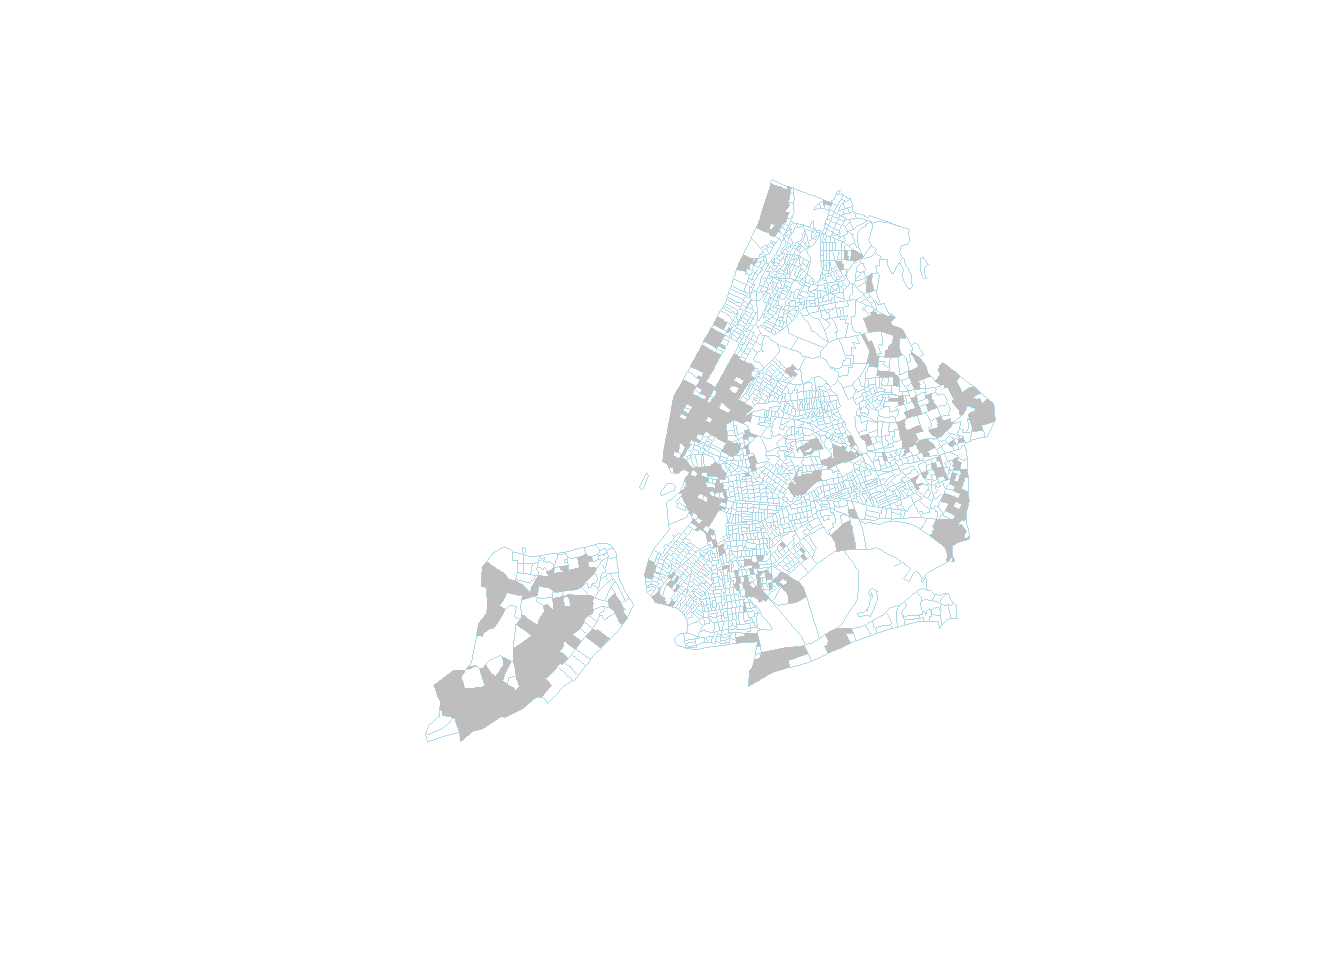
\includegraphics{R-spatial_files/figure-latex/sfAttriSelection-1.pdf}

\hypertarget{spatial-query}{%
\section{Spatial Query}\label{spatial-query}}

To perform spatial query, we must first understand spatial relationships in spatial analysis and GIScience. An excellent source for these relationships is \href{http://www.gitta.info/SpatialQueries/en/html/TopoBasedOps_learningObject1.html}{GITTA Spatial Queries}

The most useful spatial (or topological) relationships are illustrated below.

\begin{figure}
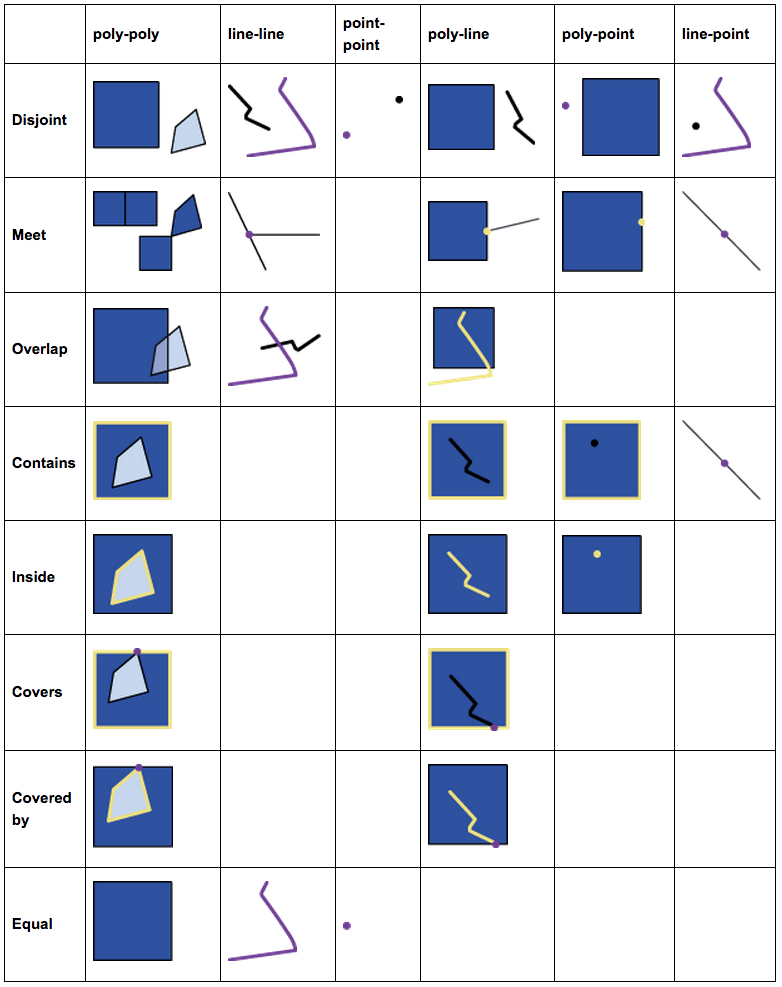
\includegraphics[width=1\linewidth]{img/topo_relations} \caption{Spatial Relations}\label{fig:topo-relations}
\end{figure}

And these basic relations form a hierarchy. For example, the \emph{intersects} relationship actually has a few subtypes like meet (or touch), overlap, and contain, etc. Anything that is not \emph{disjoint} would be an \emph{intersects}.

\begin{figure}
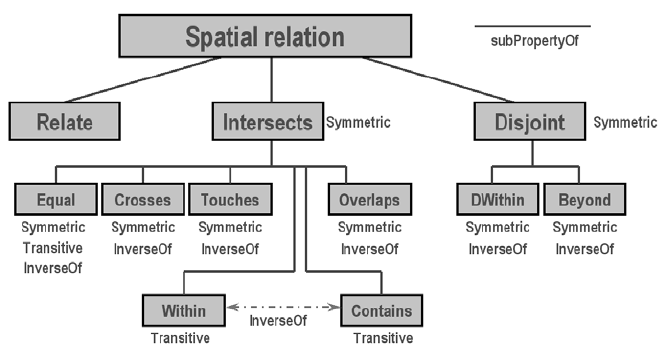
\includegraphics[width=1\linewidth]{img/spatial_relations} \caption{Hierarchy of Spatial Relations}\label{fig:spatial-relations}
\end{figure}

\begin{quote}
\textbf{\emph{Naming rules for spatial functions}}

\begin{itemize}
\tightlist
\item
  \textbf{\emph{sf}}, as well as ST\_SQL in PostGIS, uses verbs for functions of spatial relationships and use nouns for functions of spatial operations.
\item
  Spatial relationship functions like st\_overlaps, st\_covers, and st\_intersects examine the topological relationships between spatial objects.
\item
  Of course, some functions named by prepositions and adjectives like st\_within and st\_equal are only meaningful for spatial relationships.
\item
  Spatial relationship functions do not produce new geometries. They just tell use their relationships, with which we can conduct query, selection, and aggregation.
\item
  By contrast, spatial operations will create new geometries. For example, st\_intersection will produce new geometries in \textbf{\emph{sf}} classes.
\end{itemize}
\end{quote}

For the next example our goal is to select all census tracts that are adjacent to the central park.

\begin{quote}
Think about this for a moment -- what might be the steps you'd follow?
\end{quote}

\begin{Shaded}
\begin{Highlighting}[]
\DocumentationTok{\#\# How about:}

\CommentTok{\# 1. Get the census tract polygons.}
\CommentTok{\# 2. Find the census tract that contains the central park.}
\CommentTok{\# 3. Select all census tract polygons that intersect with or touch the central park tract}
\end{Highlighting}
\end{Shaded}

\hypertarget{using-the-sf-package}{%
\subsection{\texorpdfstring{Using the \emph{sf} package}{Using the sf package}}\label{using-the-sf-package}}

We will use \texttt{nyc\_sf\_merged} for the census tract polygons. Using a desktop GIS or \texttt{mapview} package in R, we can easily find out the GEOID of the central park tract is 36061014300.

First, let's use non-spatial query to find the central park census tract.

\begin{Shaded}
\begin{Highlighting}[]
\CommentTok{\# Note the GEOID column is a numeric type.}
\NormalTok{central\_partk }\OtherTok{\textless{}{-}}\NormalTok{ nyc\_sf\_merged }\SpecialCharTok{\%\textgreater{}\%} \FunctionTok{filter}\NormalTok{(GEOID }\SpecialCharTok{==} \DecValTok{36061014300}\NormalTok{)}
\end{Highlighting}
\end{Shaded}

Now we can use this \texttt{central\_park} to select all census tract polygons that intersect with the tract. In order to determine the polygons we use \texttt{st\_intersects}, a geometric binary which returns a vector of logical values, which we we can use for subsetting. Note the difference to \texttt{st\_intersection}, which performs a geometric operation and creates a new \textbf{\emph{sf}} object which cuts out the area of the buffer from the polygons a like cookie cutter.

Let us try this:

\begin{Shaded}
\begin{Highlighting}[]
\NormalTok{central\_park\_intersects }\OtherTok{\textless{}{-}} \FunctionTok{st\_intersects}\NormalTok{(central\_partk, nyc\_sf\_merged)}
\FunctionTok{class}\NormalTok{(central\_park\_intersects)}
\end{Highlighting}
\end{Shaded}

We have created a \texttt{sgbp} object, which is a ``Sparse Geometry Binary Predicate''. It is a so called sparse matrix, which is a list with integer vectors only holding the indices for each polygon that intersects. In our case we only have one vector, because we only intersect with one buffer polygon, so we can extract this first vector with \texttt{philly\_buf\_intersects{[}{[}1{]}{]}} and use it for subsetting:

\begin{Shaded}
\begin{Highlighting}[]
\CommentTok{\# Subsetting using the results}
\NormalTok{nyc\_sel\_sf }\OtherTok{\textless{}{-}}\NormalTok{ nyc\_sf\_merged[central\_park\_intersects[[}\DecValTok{1}\NormalTok{]],]}
\CommentTok{\# or in tidyverse style}
\NormalTok{nyc\_sel\_sf }\OtherTok{\textless{}{-}}\NormalTok{ nyc\_sf\_merged }\SpecialCharTok{\%\textgreater{}\%}\NormalTok{ dplyr}\SpecialCharTok{::}\FunctionTok{slice}\NormalTok{(central\_park\_intersects[[}\DecValTok{1}\NormalTok{]])}


\CommentTok{\# plot}
\FunctionTok{plot}\NormalTok{(}\FunctionTok{st\_geometry}\NormalTok{(nyc\_sf\_merged), }\AttributeTok{border=}\StringTok{"\#aaaaaa"}\NormalTok{, }\AttributeTok{main=}\StringTok{"Census tracts near Central Park"}\NormalTok{)}
\FunctionTok{plot}\NormalTok{(}\FunctionTok{st\_geometry}\NormalTok{(nyc\_sel\_sf), }\AttributeTok{add=}\NormalTok{T, }\AttributeTok{col=}\StringTok{"lightpink"}\NormalTok{)}
\FunctionTok{plot}\NormalTok{(}\FunctionTok{st\_geometry}\NormalTok{(nyc\_sel\_sf), }\AttributeTok{add=}\NormalTok{T, }\AttributeTok{col=}\ConstantTok{NA}\NormalTok{, }\AttributeTok{border=} \StringTok{\textquotesingle{}lightgrey\textquotesingle{}}\NormalTok{,}\AttributeTok{lwd =} \DecValTok{1}\NormalTok{)}
\end{Highlighting}
\end{Shaded}

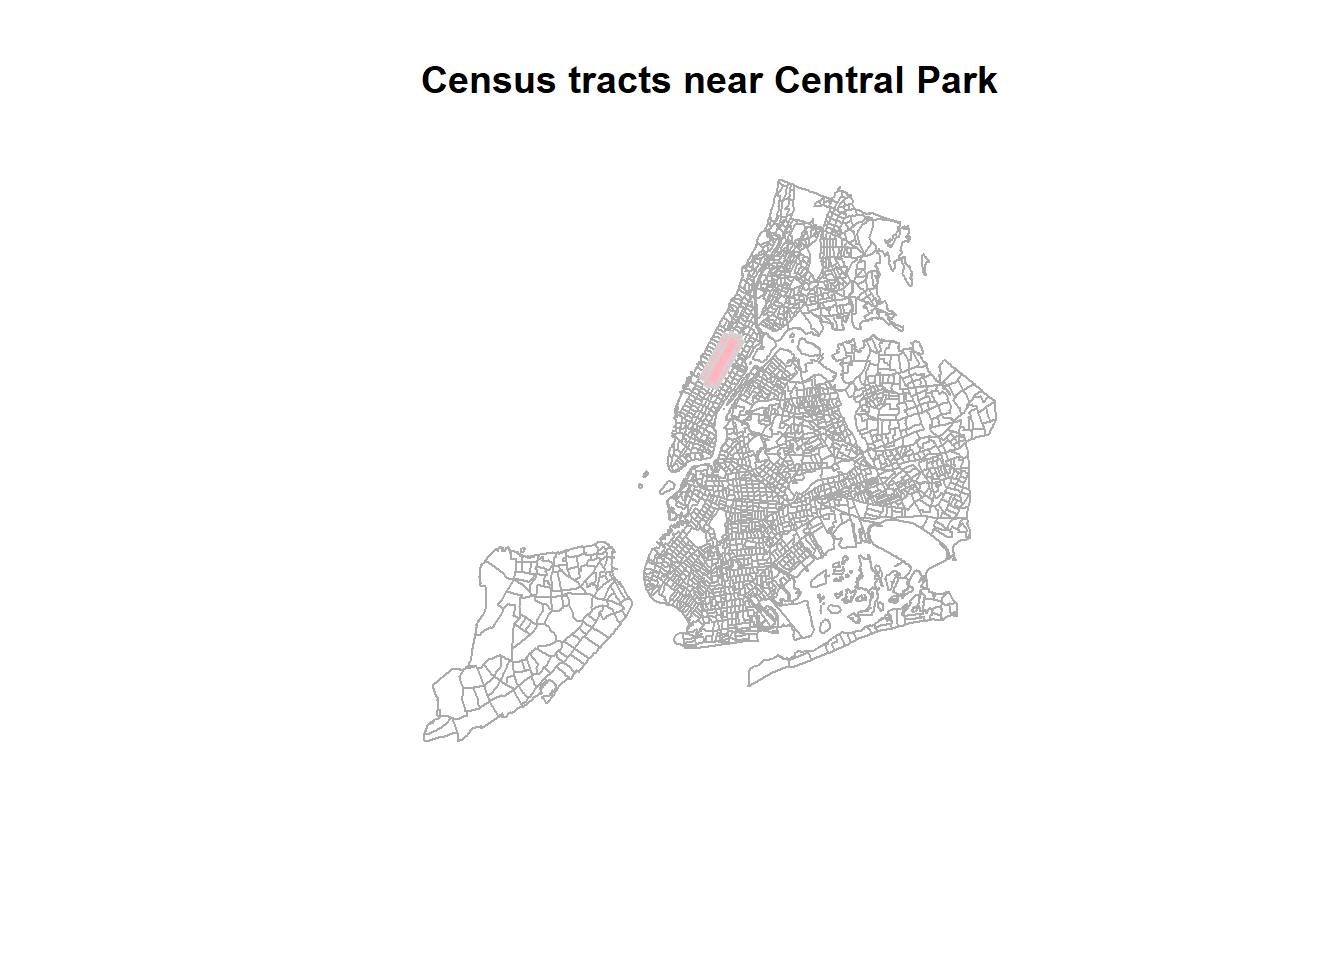
\includegraphics{R-spatial_files/figure-latex/sf-intersection-subset-1.pdf}

\begin{Shaded}
\begin{Highlighting}[]
\CommentTok{\# or Interactive map using mapview}
\FunctionTok{mapview}\NormalTok{(nyc\_sel\_sf)}
\end{Highlighting}
\end{Shaded}

\hypertarget{reprojecting-or-projection-transform}{%
\section{Reprojecting or Projection Transform}\label{reprojecting-or-projection-transform}}

Occasionally we may have to change the coordinates of our spatial object into a new Coordinate Reference System (CRS).

\hypertarget{transform-or-reproject-sf-objects-1}{%
\subsection{\texorpdfstring{Transform or reproject \textbf{\emph{sf}} objects}{Transform or reproject sf objects}}\label{transform-or-reproject-sf-objects-1}}

Let us check \texttt{nyc\_sf\_merged} object and reproject it to a local projection in State Plane Long Island, that is the local map projection the NYC.

\begin{Shaded}
\begin{Highlighting}[]
\FunctionTok{st\_crs}\NormalTok{(nyc\_sf\_merged)}
\end{Highlighting}
\end{Shaded}

\begin{verbatim}
#> Coordinate Reference System:
#>   User input: NAD83 
#>   wkt:
#> GEOGCRS["NAD83",
#>     DATUM["North American Datum 1983",
#>         ELLIPSOID["GRS 1980",6378137,298.257222101,
#>             LENGTHUNIT["metre",1]]],
#>     PRIMEM["Greenwich",0,
#>         ANGLEUNIT["degree",0.0174532925199433]],
#>     CS[ellipsoidal,2],
#>         AXIS["latitude",north,
#>             ORDER[1],
#>             ANGLEUNIT["degree",0.0174532925199433]],
#>         AXIS["longitude",east,
#>             ORDER[2],
#>             ANGLEUNIT["degree",0.0174532925199433]],
#>     ID["EPSG",4269]]
\end{verbatim}

\begin{Shaded}
\begin{Highlighting}[]
\CommentTok{\# then we transform/reproject it to SPCS Long Island, 2831}
\NormalTok{nyc\_sf\_2831 }\OtherTok{\textless{}{-}} \FunctionTok{st\_transform}\NormalTok{(nyc\_sf\_merged, }\DecValTok{2831}\NormalTok{)}
\FunctionTok{st\_crs}\NormalTok{(nyc\_sf\_2831)}
\end{Highlighting}
\end{Shaded}

\begin{verbatim}
#> Coordinate Reference System:
#>   User input: EPSG:2831 
#>   wkt:
#> PROJCRS["NAD83(HARN) / New York Long Island",
#>     BASEGEOGCRS["NAD83(HARN)",
#>         DATUM["NAD83 (High Accuracy Reference Network)",
#>             ELLIPSOID["GRS 1980",6378137,298.257222101,
#>                 LENGTHUNIT["metre",1]]],
#>         PRIMEM["Greenwich",0,
#>             ANGLEUNIT["degree",0.0174532925199433]],
#>         ID["EPSG",4152]],
#>     CONVERSION["SPCS83 New York Long Island zone (meters)",
#>         METHOD["Lambert Conic Conformal (2SP)",
#>             ID["EPSG",9802]],
#>         PARAMETER["Latitude of false origin",40.1666666666667,
#>             ANGLEUNIT["degree",0.0174532925199433],
#>             ID["EPSG",8821]],
#>         PARAMETER["Longitude of false origin",-74,
#>             ANGLEUNIT["degree",0.0174532925199433],
#>             ID["EPSG",8822]],
#>         PARAMETER["Latitude of 1st standard parallel",41.0333333333333,
#>             ANGLEUNIT["degree",0.0174532925199433],
#>             ID["EPSG",8823]],
#>         PARAMETER["Latitude of 2nd standard parallel",40.6666666666667,
#>             ANGLEUNIT["degree",0.0174532925199433],
#>             ID["EPSG",8824]],
#>         PARAMETER["Easting at false origin",300000,
#>             LENGTHUNIT["metre",1],
#>             ID["EPSG",8826]],
#>         PARAMETER["Northing at false origin",0,
#>             LENGTHUNIT["metre",1],
#>             ID["EPSG",8827]]],
#>     CS[Cartesian,2],
#>         AXIS["easting (X)",east,
#>             ORDER[1],
#>             LENGTHUNIT["metre",1]],
#>         AXIS["northing (Y)",north,
#>             ORDER[2],
#>             LENGTHUNIT["metre",1]],
#>     USAGE[
#>         SCOPE["Engineering survey, topographic mapping."],
#>         AREA["United States (USA) - New York - counties of Bronx; Kings; Nassau; New York; Queens; Richmond; Suffolk."],
#>         BBOX[40.47,-74.26,41.3,-71.8]],
#>     ID["EPSG",2831]]
\end{verbatim}

We see that the CRS are different for the two. One is geographic coordinate systems (longitude, latitude) using NAD83 and the other is New York State Plane Long Island.

We can also see the proj4 strings of the two.

\begin{Shaded}
\begin{Highlighting}[]
\FunctionTok{st\_crs}\NormalTok{(nyc\_sf\_merged)}\SpecialCharTok{$}\NormalTok{proj4string}
\FunctionTok{st\_crs}\NormalTok{(nyc\_sf\_2831)}\SpecialCharTok{$}\NormalTok{proj4string}
\end{Highlighting}
\end{Shaded}

: we have \texttt{+proj=lcc...} and \texttt{+proj=longlat...}. LCC refers to Lambert Conic Conformal, which is a projected coordinate system with numeric units.

We can use the \texttt{st\_bbox()} method from the \emph{sf} package to compare the coordinates before and after transformation and confirm that we actually have transformed them. \texttt{st\_bbox()} returns the \emph{min} and \emph{max} values of the two dimensions of a \emph{sf} spatial object.

\begin{Shaded}
\begin{Highlighting}[]
\NormalTok{sf}\SpecialCharTok{::}\FunctionTok{st\_bbox}\NormalTok{(nyc\_sf\_merged) }\CommentTok{\# bounding box}
\end{Highlighting}
\end{Shaded}

\begin{verbatim}
#>      xmin      ymin      xmax      ymax 
#> -74.25609  40.50203 -73.70002  40.91758
\end{verbatim}

\begin{Shaded}
\begin{Highlighting}[]
\FunctionTok{st\_bbox}\NormalTok{(nyc\_sf\_2831)}
\end{Highlighting}
\end{Shaded}

\begin{verbatim}
#>      xmin      ymin      xmax      ymax 
#> 278294.41  37271.09 325338.38  83388.58
\end{verbatim}

We can also compare them visually with:

\begin{Shaded}
\begin{Highlighting}[]
\FunctionTok{par}\NormalTok{(}\AttributeTok{mfrow=}\FunctionTok{c}\NormalTok{(}\DecValTok{1}\NormalTok{,}\DecValTok{2}\NormalTok{)) }
\FunctionTok{plot}\NormalTok{(}\FunctionTok{st\_geometry}\NormalTok{(nyc\_sf\_merged), }\AttributeTok{axes=}\ConstantTok{TRUE}\NormalTok{, }\AttributeTok{main =} \StringTok{"before transform {-} latlon"}\NormalTok{)}
\FunctionTok{plot}\NormalTok{(}\FunctionTok{st\_geometry}\NormalTok{(nyc\_sf\_2831), }\AttributeTok{axes=}\ConstantTok{TRUE}\NormalTok{, }\AttributeTok{main =} \StringTok{"after transform {-} lcc"}\NormalTok{)}
\end{Highlighting}
\end{Shaded}

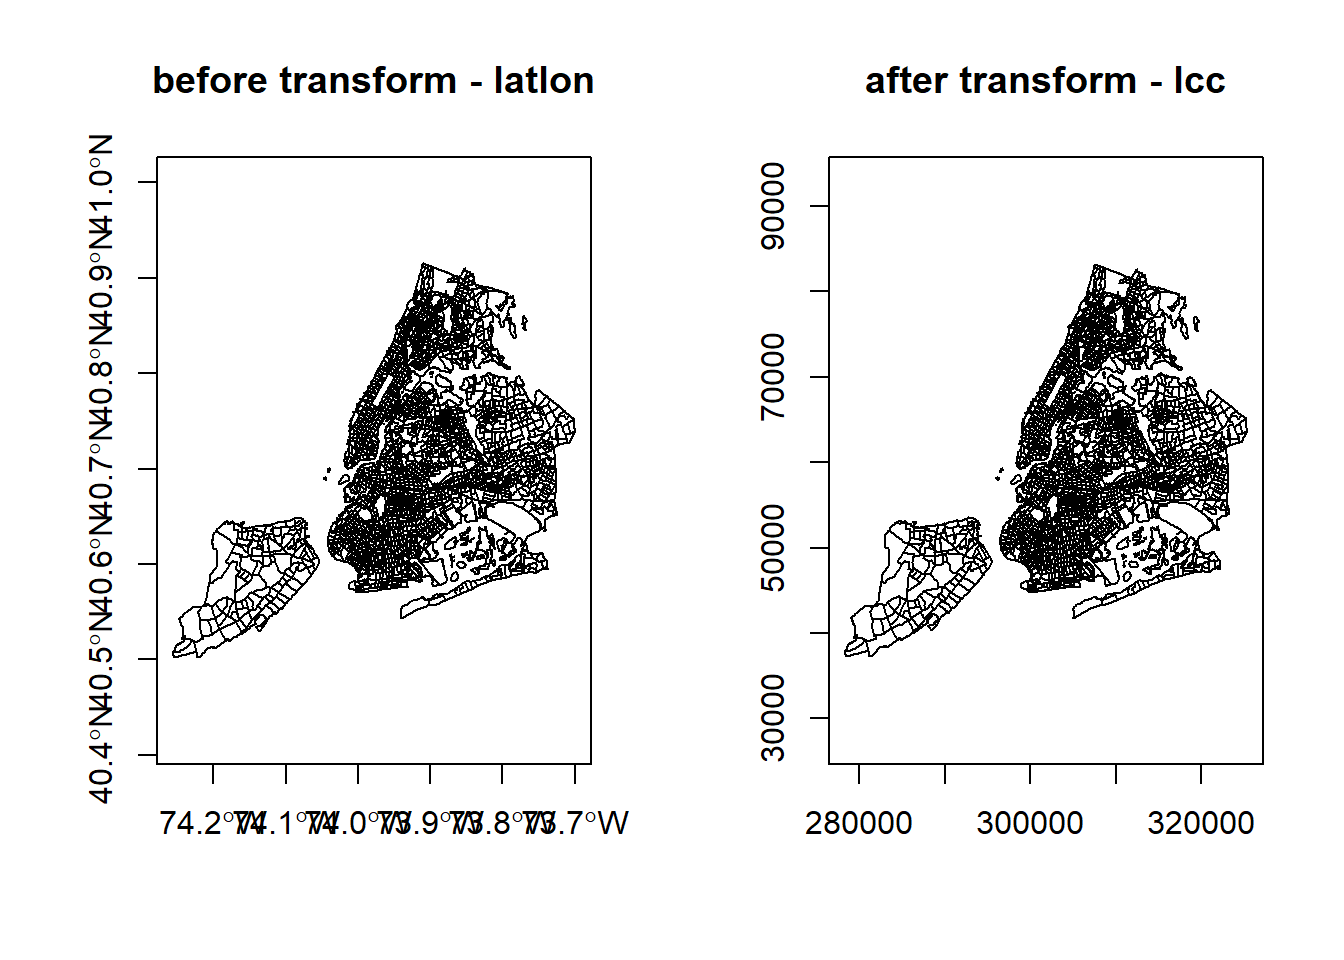
\includegraphics{R-spatial_files/figure-latex/compare-reproj-plots-sf-1.pdf}

Lastly, let us save the reprojected file as \texttt{nyc\_tracts\_2831} shapefile, as we may use it later on.

\begin{Shaded}
\begin{Highlighting}[]
\FunctionTok{st\_write}\NormalTok{(nyc\_sf\_2831, }\StringTok{\textquotesingle{}data/nyc/nyc\_tracts\_2831.shp\textquotesingle{}}\NormalTok{)}
\end{Highlighting}
\end{Shaded}

\begin{quote}
\textbf{\emph{Set CRS and Reproject (transform)}}
\end{quote}

\begin{itemize}
\tightlist
\item
  Assigning a new CRS to a spatial object does not change its coordinates but the CRS determines how the software understand the coordinates. So, we must choose and set a CRS that is consistent with the coordinates. Otherwise, the coordinates will be misinterpreted.
\item
  Reprojecting spatial data with st\_transform and gTransform really changes the underlying coordinates, which we can see from the bbox values.\\
\item
  In either case, the CRS must be consistent with the coordinates. It is a good practice to check projected spatial data against a basemap or a correctly referenced map to verify its CRS.
\item
  \href{https://spatialreference.org/}{SpatialReference.org} is a very good source for CRS information.
\item
  Some commonly used reference systems

  \begin{itemize}
  \tightlist
  \item
    US 48 Contiguous States: Albers Equal Area (ESRI:102003), Lambert Conformal (ESRI:102004)
  \item
    New York State: UTM 18N (EPSG 3725, 3748, 26918)
  \item
    New York City: State Plane Long Island (EPSG 2263, 2831, 3627)
  \end{itemize}
\end{itemize}

\hypertarget{spatial-query-with-reprojection}{%
\subsection{Spatial Query with Reprojection}\label{spatial-query-with-reprojection}}

Another scenario where we need to transform spatial data into a different projection is to apply distances. This is because local projections tend to minimize distortion and they also use units like meter or feet. Here we use a distance buffer example to illustrate both transformation/reprojection and spatial query. In this example, we try to find the noise complaint within 200 meter from Hunter College, 09/01/2019 to 09/01/2020.

First, we search the geographic coordinates of Hunter College and find (-73.9645, 40.7678). Then, we create a spatial object for this location. As we don't really use any attribute information for this location, a \texttt{sfc} object is sufficient.

\begin{Shaded}
\begin{Highlighting}[]
\CommentTok{\# make a simple feature point with CRS}
\NormalTok{hunter\_college\_sfc }\OtherTok{\textless{}{-}} \FunctionTok{st\_sfc}\NormalTok{(}\FunctionTok{st\_point}\NormalTok{(}\FunctionTok{c}\NormalTok{(}\SpecialCharTok{{-}}\FloatTok{73.9645}\NormalTok{, }\FloatTok{40.7678}\NormalTok{)), }\AttributeTok{crs =} \DecValTok{4269}\NormalTok{)}
\CommentTok{\# Verify the location using mapview with basemap or ggmaps}
\FunctionTok{mapview}\NormalTok{(hunter\_college\_sfc)}
\end{Highlighting}
\end{Shaded}

We can also use what we learned earlier to directly create a \emph{sf} object.

\begin{Shaded}
\begin{Highlighting}[]
\CommentTok{\# make a simple feature point with CRS}
\NormalTok{hunter\_college\_sf }\OtherTok{\textless{}{-}} \FunctionTok{st\_as\_sf}\NormalTok{(}\FunctionTok{data.frame}\NormalTok{(}\AttributeTok{x=}\SpecialCharTok{{-}}\FloatTok{73.9645}\NormalTok{, }\AttributeTok{y=}\FloatTok{40.7678}\NormalTok{), }\AttributeTok{coords =} \FunctionTok{c}\NormalTok{(}\StringTok{\textquotesingle{}x\textquotesingle{}}\NormalTok{,}\StringTok{\textquotesingle{}y\textquotesingle{}}\NormalTok{), }\AttributeTok{crs =} \DecValTok{4269}\NormalTok{)}
\CommentTok{\# Verify the location using mapview with basemap or ggmaps}
\FunctionTok{mapview}\NormalTok{(hunter\_college\_sf)}
\end{Highlighting}
\end{Shaded}

Now, let's read the Manhattan noise data and check on their coordinate systems. If they have the same CRS with a unit of meter, we can use them directly. Otherwise, we have to convert them to a local map projection with a meter unit.

\begin{Shaded}
\begin{Highlighting}[]
\NormalTok{man\_noise\_sf }\OtherTok{\textless{}{-}}\NormalTok{ sf}\SpecialCharTok{::}\FunctionTok{st\_read}\NormalTok{(}\StringTok{\textquotesingle{}data/nyc/ManhattanNoise.shp\textquotesingle{}}\NormalTok{)}
\FunctionTok{st\_crs}\NormalTok{(hunter\_college\_sf)}
\FunctionTok{st\_crs}\NormalTok{(man\_noise\_sf)}
\end{Highlighting}
\end{Shaded}

It turns out both use geographic coordiantes with a unit of decimal degree. But one is using WGS84 (4326) and the other is using NAD83 (4326). Although they are very similar to each other, none of them have a unit of meter. So, we must convert both to the same CRS using New York Long Island (State Plain Coordinate System, SPCS) with a unit of meter. The SRID is 2831. Note 2263 is also New York Long Island, but its unit is feet.

To avoid saving all the intermediate results, we use pipe \texttt{\%\textgreater{}\%} to get the buffer and to conduct the spatial query.

\begin{Shaded}
\begin{Highlighting}[]
\NormalTok{  hunter\_college\_sf }\SpecialCharTok{\%\textgreater{}\%}\NormalTok{ sf}\SpecialCharTok{::}\FunctionTok{st\_transform}\NormalTok{(}\DecValTok{2831}\NormalTok{) }\SpecialCharTok{\%\textgreater{}\%} \CommentTok{\# transform the data to 2831}
\NormalTok{    sf}\SpecialCharTok{::}\FunctionTok{st\_buffer}\NormalTok{(}\DecValTok{200}\NormalTok{) }\SpecialCharTok{\%\textgreater{}\%} \CommentTok{\# create the buffer}
\NormalTok{    sf}\SpecialCharTok{::}\FunctionTok{st\_intersects}\NormalTok{(man\_noise\_sf }\CommentTok{\# intersects with the transformed noise data}
                        \SpecialCharTok{\%\textgreater{}\%} \FunctionTok{st\_transform}\NormalTok{(}\DecValTok{2831}\NormalTok{)) }\SpecialCharTok{\%\textgreater{}\%} 
\NormalTok{    magrittr}\SpecialCharTok{::}\FunctionTok{extract2}\NormalTok{(., }\DecValTok{1}\NormalTok{) }\SpecialCharTok{\%\textgreater{}\%} \CommentTok{\# Get the indices of the noise points within 200 meter buffer}
\NormalTok{    dplyr}\SpecialCharTok{::}\FunctionTok{slice}\NormalTok{(man\_noise\_sf, .) }\SpecialCharTok{\%\textgreater{}\%} \CommentTok{\# Get those noise points}
\NormalTok{    mapview}\SpecialCharTok{::}\FunctionTok{mapview}\NormalTok{() }\CommentTok{\# Map them out using a simple interactive map}
\end{Highlighting}
\end{Shaded}

This chunk of code may be difficult to understand. You can break it down and explicitly save the intermediate data using variables.

\hypertarget{raster-reprojection}{%
\subsection{Raster reprojection}\label{raster-reprojection}}

Here is what it would look like to reproject the HARV raster used earlier to a WGS84 projection. We see that the original projection is in UTM.

\begin{Shaded}
\begin{Highlighting}[]
\CommentTok{\# if you need to load again:}
\CommentTok{\#HARV \textless{}{-} raster("data/HARV\_RGB\_Ortho.tif")}
\NormalTok{raster}\SpecialCharTok{::}\FunctionTok{crs}\NormalTok{(HARV)}
\end{Highlighting}
\end{Shaded}

\begin{verbatim}
#> Coordinate Reference System:
#> Deprecated Proj.4 representation:
#>  +proj=utm +zone=18 +datum=WGS84 +units=m +no_defs 
#> WKT2 2019 representation:
#> PROJCRS["WGS 84 / UTM zone 18N",
#>     BASEGEOGCRS["WGS 84",
#>         DATUM["World Geodetic System 1984",
#>             ELLIPSOID["WGS 84",6378137,298.257223563,
#>                 LENGTHUNIT["metre",1]]],
#>         PRIMEM["Greenwich",0,
#>             ANGLEUNIT["degree",0.0174532925199433]],
#>         ID["EPSG",4326]],
#>     CONVERSION["UTM zone 18N",
#>         METHOD["Transverse Mercator",
#>             ID["EPSG",9807]],
#>         PARAMETER["Latitude of natural origin",0,
#>             ANGLEUNIT["degree",0.0174532925199433],
#>             ID["EPSG",8801]],
#>         PARAMETER["Longitude of natural origin",-75,
#>             ANGLEUNIT["degree",0.0174532925199433],
#>             ID["EPSG",8802]],
#>         PARAMETER["Scale factor at natural origin",0.9996,
#>             SCALEUNIT["unity",1],
#>             ID["EPSG",8805]],
#>         PARAMETER["False easting",500000,
#>             LENGTHUNIT["metre",1],
#>             ID["EPSG",8806]],
#>         PARAMETER["False northing",0,
#>             LENGTHUNIT["metre",1],
#>             ID["EPSG",8807]]],
#>     CS[Cartesian,2],
#>         AXIS["(E)",east,
#>             ORDER[1],
#>             LENGTHUNIT["metre",1]],
#>         AXIS["(N)",north,
#>             ORDER[2],
#>             LENGTHUNIT["metre",1]],
#>     USAGE[
#>         SCOPE["Engineering survey, topographic mapping."],
#>         AREA["Between 78°W and 72°W, northern hemisphere between equator and 84°N, onshore and offshore. Bahamas. Canada - Nunavut; Ontario; Quebec. Colombia. Cuba. Ecuador. Greenland. Haiti. Jamica. Panama. Turks and Caicos Islands. United States (USA). Venezuela."],
#>         BBOX[0,-78,84,-72]],
#>     ID["EPSG",32618]]
\end{verbatim}

\begin{Shaded}
\begin{Highlighting}[]
\NormalTok{HARV\_WGS84 }\OtherTok{\textless{}{-}} \FunctionTok{projectRaster}\NormalTok{(HARV, }\AttributeTok{crs=}\FunctionTok{CRS}\NormalTok{(}\StringTok{"+proj=longlat +datum=WGS84"}\NormalTok{))}
\end{Highlighting}
\end{Shaded}

Let's look at the coordinates to see the effect:

\begin{Shaded}
\begin{Highlighting}[]
\FunctionTok{extent}\NormalTok{(HARV)}
\end{Highlighting}
\end{Shaded}

\begin{verbatim}
#> class      : Extent 
#> xmin       : 731998.5 
#> xmax       : 732766.8 
#> ymin       : 4712956 
#> ymax       : 4713536
\end{verbatim}

\begin{Shaded}
\begin{Highlighting}[]
\FunctionTok{extent}\NormalTok{(HARV\_WGS84)}
\end{Highlighting}
\end{Shaded}

\begin{verbatim}
#> class      : Extent 
#> xmin       : -72.17505 
#> xmax       : -72.16544 
#> ymin       : 42.53393 
#> ymax       : 42.5394
\end{verbatim}

\begin{Shaded}
\begin{Highlighting}[]
\FunctionTok{ncell}\NormalTok{(HARV)}
\end{Highlighting}
\end{Shaded}

\begin{verbatim}
#> [1] 7120141
\end{verbatim}

\begin{Shaded}
\begin{Highlighting}[]
\FunctionTok{ncell}\NormalTok{(HARV\_WGS84)}
\end{Highlighting}
\end{Shaded}

\begin{verbatim}
#> [1] 7687552
\end{verbatim}

And here is the visual proof:

\begin{Shaded}
\begin{Highlighting}[]
\FunctionTok{plot}\NormalTok{(HARV, }\AttributeTok{main =} \StringTok{"before transform {-} UTM"}\NormalTok{)}
\end{Highlighting}
\end{Shaded}

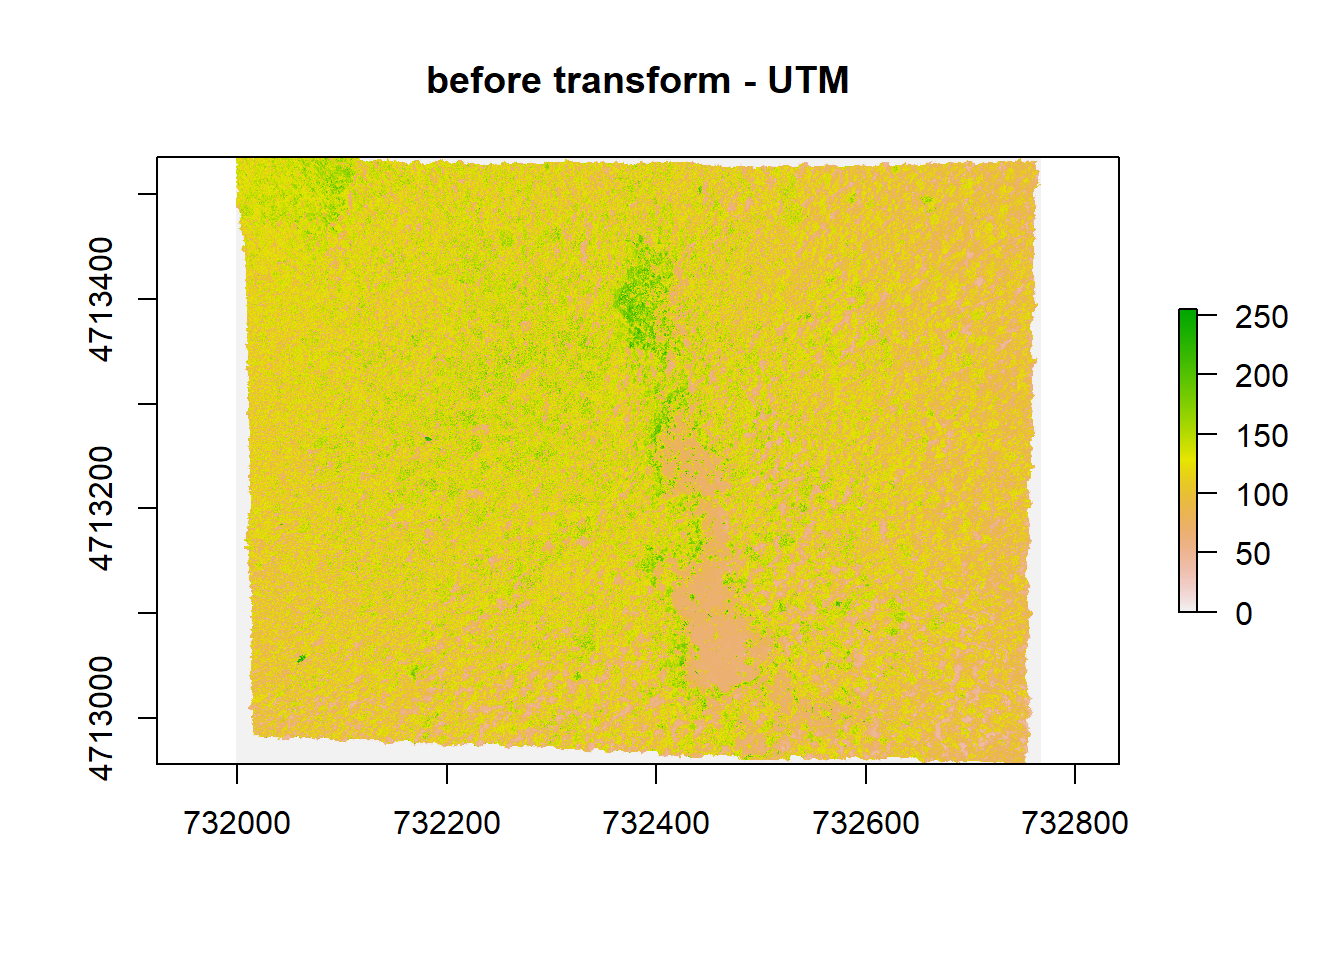
\includegraphics{R-spatial_files/figure-latex/raster-reproject-plot1-1.pdf}

\begin{Shaded}
\begin{Highlighting}[]
\FunctionTok{plot}\NormalTok{(HARV\_WGS84, }\AttributeTok{main =} \StringTok{"after transform {-} WGS84"}\NormalTok{)}
\end{Highlighting}
\end{Shaded}

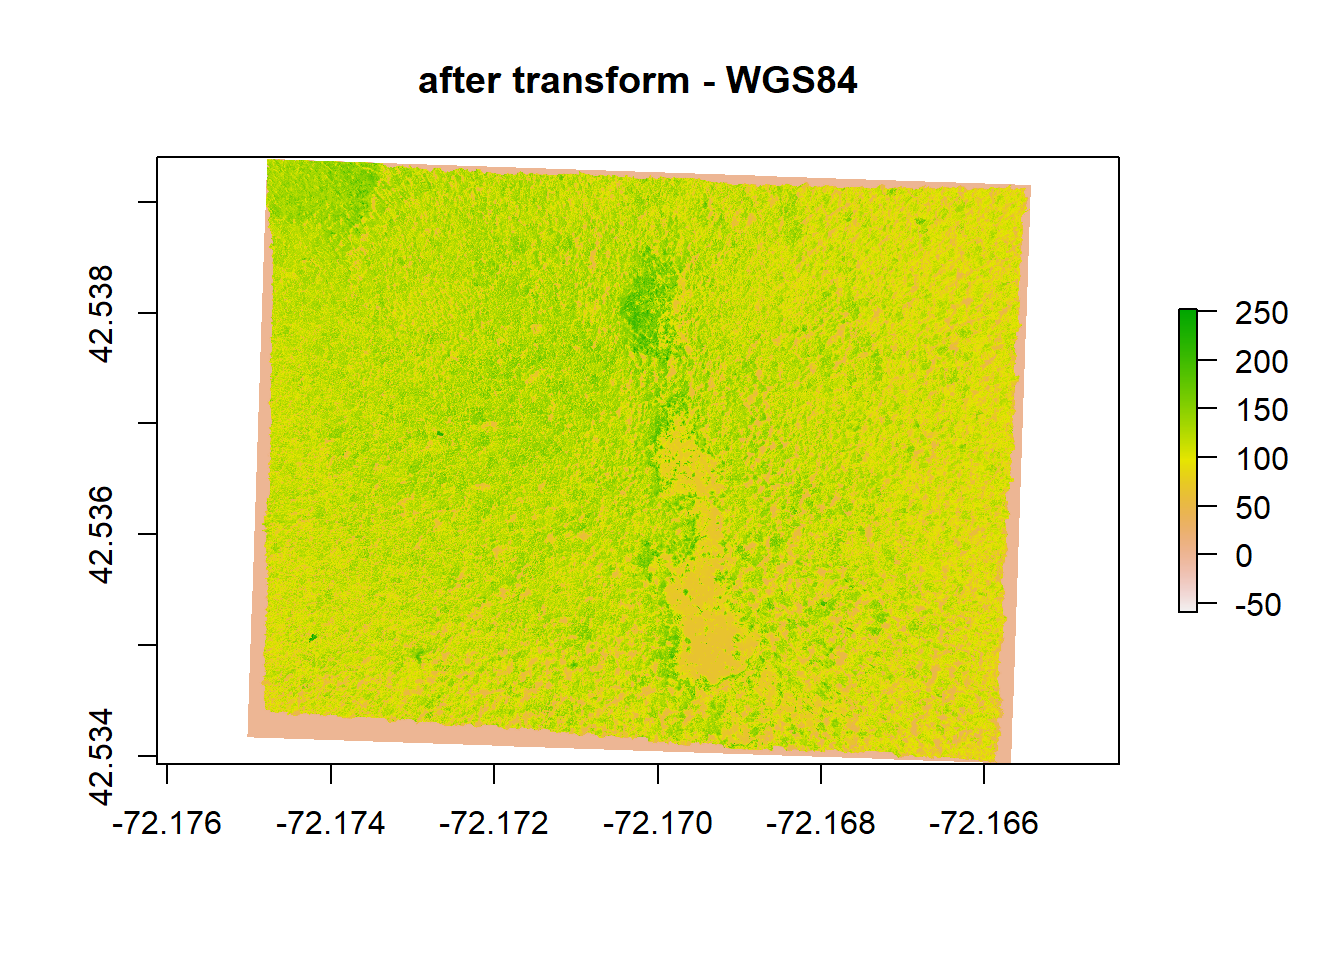
\includegraphics{R-spatial_files/figure-latex/raster-reproject-plot2-1.pdf}

\hypertarget{spatial-join-and-aggregation-points-in-polygons}{%
\section{Spatial Join and Aggregation: Points in Polygons}\label{spatial-join-and-aggregation-points-in-polygons}}

Now that we have both noise and census tracts we will forge ahead and ask for the density of noise complaint for \textbf{each census tract} in Manhattan: \(\frac{{noise complaints}}{area}\)

To achieve this this we join the points of noise complaints to the census tract polygon and count them up for each polygon. You might be familiar with this operation from ArcGIS, QGIS, or other GIS packages. Note that for topological relationships not based on distances, it will work as long as both data have the same coordinate systems.

\hypertarget{with-sf-1}{%
\subsection{\texorpdfstring{With \emph{sf}}{With sf}}\label{with-sf-1}}

We will use piping and build up our object in the following way. First we calculate the area for each tract. We use the \texttt{st\_area} function on the geometry column and add the result.

\begin{Shaded}
\begin{Highlighting}[]
\NormalTok{nyc\_census\_tracts\_sf }\SpecialCharTok{\%\textgreater{}\%} 
  \FunctionTok{filter}\NormalTok{(COUNTYFP }\SpecialCharTok{==} \StringTok{\textquotesingle{}061\textquotesingle{}}\NormalTok{) }\SpecialCharTok{\%\textgreater{}\%}
  \FunctionTok{mutate}\NormalTok{(}\AttributeTok{tract\_area =} \FunctionTok{st\_area}\NormalTok{(geometry)) }\SpecialCharTok{\%\textgreater{}\%} 
  \FunctionTok{head}\NormalTok{()}
\end{Highlighting}
\end{Shaded}

Next, we use st\_join to perform a spatial join with the points:

\begin{Shaded}
\begin{Highlighting}[]
\NormalTok{nyc\_census\_tracts\_sf }\SpecialCharTok{\%\textgreater{}\%} 
  \FunctionTok{filter}\NormalTok{(COUNTYFP }\SpecialCharTok{==} \StringTok{\textquotesingle{}061\textquotesingle{}}\NormalTok{) }\SpecialCharTok{\%\textgreater{}\%}
  \FunctionTok{mutate}\NormalTok{(}\AttributeTok{tract\_area =} \FunctionTok{st\_area}\NormalTok{(geometry)) }\SpecialCharTok{\%\textgreater{}\%} 
  \FunctionTok{st\_transform}\NormalTok{(}\DecValTok{4326}\NormalTok{) }\SpecialCharTok{\%\textgreater{}\%}
  \FunctionTok{st\_join}\NormalTok{(man\_noise\_sf) }\SpecialCharTok{\%\textgreater{}\%}
  \FunctionTok{head}\NormalTok{()}
\end{Highlighting}
\end{Shaded}

Now we can group by a variable that unique identifies the census tracts, (we choose \emph{GEOID}) and use \texttt{summarize} to count the points for each tract and calculate the rate of noise complaints. Since our units are in sq meter. multiply by by 1000000 to get sq km. We also need to carry over the area, which we can use \texttt{max}, \texttt{min}, \texttt{mean}, or \texttt{unique} as all the values are the same for the same census tract.

We also assign the output to a new object \texttt{crime\_rate}.

\begin{Shaded}
\begin{Highlighting}[]
\NormalTok{noise\_rate\_sf }\OtherTok{\textless{}{-}}\NormalTok{ nyc\_census\_tracts\_sf }\SpecialCharTok{\%\textgreater{}\%} 
      \FunctionTok{filter}\NormalTok{(COUNTYFP }\SpecialCharTok{==} \StringTok{\textquotesingle{}061\textquotesingle{}}\NormalTok{) }\SpecialCharTok{\%\textgreater{}\%}
      \FunctionTok{mutate}\NormalTok{(}\AttributeTok{tract\_area =} \FunctionTok{st\_area}\NormalTok{(geometry)) }\SpecialCharTok{\%\textgreater{}\%}
      \FunctionTok{st\_transform}\NormalTok{(}\DecValTok{4326}\NormalTok{) }\SpecialCharTok{\%\textgreater{}\%}
      \FunctionTok{st\_join}\NormalTok{(man\_noise\_sf) }\SpecialCharTok{\%\textgreater{}\%}
      \FunctionTok{group\_by}\NormalTok{(GEOID) }\SpecialCharTok{\%\textgreater{}\%} 
      \FunctionTok{summarize}\NormalTok{(}\AttributeTok{n\_noise =} \FunctionTok{n}\NormalTok{(),}
                \AttributeTok{tract\_area =} \FunctionTok{max}\NormalTok{(tract\_area),}
                \AttributeTok{noise\_rate =}\NormalTok{ n\_noise}\SpecialCharTok{/}\NormalTok{tract\_area }\SpecialCharTok{*} \FloatTok{1e6}\NormalTok{) }
\end{Highlighting}
\end{Shaded}

And here is a simple plot:

\begin{Shaded}
\begin{Highlighting}[]
\FunctionTok{mapview}\NormalTok{(noise\_rate\_sf, }\AttributeTok{zcol=}\StringTok{\textquotesingle{}noise\_rate\textquotesingle{}}\NormalTok{, }\AttributeTok{legend=}\ConstantTok{FALSE}\NormalTok{)}
\end{Highlighting}
\end{Shaded}

Finally, we write this out for later:

\begin{Shaded}
\begin{Highlighting}[]
\FunctionTok{st\_write}\NormalTok{(noise\_rate\_sf, }\StringTok{"data/nyc/man\_noise\_rate.shp"}\NormalTok{)}
\end{Highlighting}
\end{Shaded}

\hypertarget{sp---sf-comparison}{%
\subsection{\texorpdfstring{\emph{sp} - \emph{sf} comparison}{sp - sf comparison}}\label{sp---sf-comparison}}

\begin{longtable}[]{@{}lll@{}}
\toprule
how to.. & for \emph{sp} objects & for \emph{sf} objects \\
\midrule
\endhead
join attributes & \texttt{sp::merge()} & \texttt{dplyr::*\_join()} (also \texttt{sf::merge()}) \\
reproject & \texttt{spTransform()} & \texttt{st\_transform()} \\
retrieve (or assign) CRS & \texttt{proj4string()} & \texttt{st\_crs()} \\
count points in polygons & \texttt{aggregate()} or \texttt{over()} & \texttt{st\_within()} or \texttt{aggregate()} \\
buffer & \texttt{rgeos::gBuffer()} (separate package) & \texttt{st\_buffer()} \\
select by location & \href{https://www.rdocumentation.org/packages/rgeos/}{\texttt{g*} functions} from \texttt{rgeos} & \href{https://www.rdocumentation.org/packages/sf/topics/geos}{st\_* geos functions} in \emph{sf} \\
\bottomrule
\end{longtable}

Here are some additional packages that use vector data:

\begin{itemize}
\tightlist
\item
  \href{https://CRAN.R-project.org/package=stplanr}{\texttt{stplanr}}: Functionality and data access tools for transport planning, including origin-destination analysis, route allocation and modelling travel patterns.
\item
  \href{https://CRAN.R-project.org/package=bikedata}{\texttt{bikedata}}: Data from public hire bicycle systems,including London, New York, Chicago, Washington DC, Boston, Los Angeles, and Philadelphia
\end{itemize}

\hypertarget{spatial-operations}{%
\section{Spatial Operations}\label{spatial-operations}}

\hypertarget{spatial-measures}{%
\subsection{Spatial Measures}\label{spatial-measures}}

This type of operations measure certain values from spatial objects. For example, we can derive the boundary box and centroid using \texttt{sf::st\_bbox} and \texttt{sf::st\_centroid}. More basic measures are areas and length with \texttt{sf::st\_area} and \texttt{sf::st\_length}.

\hypertarget{geometric-operations}{%
\subsection{Geometric Operations}\label{geometric-operations}}

More interestingly, we can conduct certain geometric operations such as buffer and overlay. In spatial analysis, overlay contains a few types.

\begin{figure}
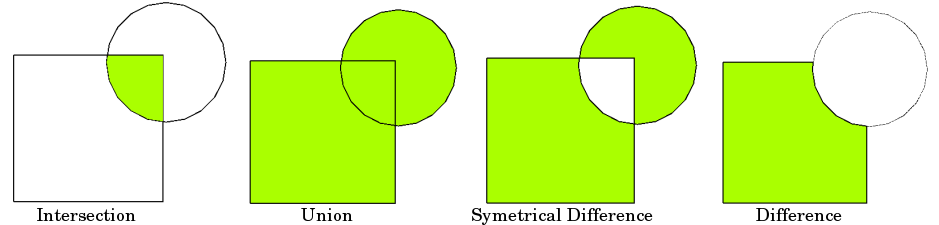
\includegraphics[width=1\linewidth]{img/overlay_operations} \caption{Overlay Types}\label{fig:overlay-types}
\end{figure}

And \href{https://saylordotorg.github.io/text_essentials-of-geographic-information-systems/s11-geospatial-analysis-i-vector-o.html}{this web page} has an excellent explanation to the spatial operations on vector data, including buffer, operations involving one (unary) or multiple layers of spatial objects.

\begin{figure}
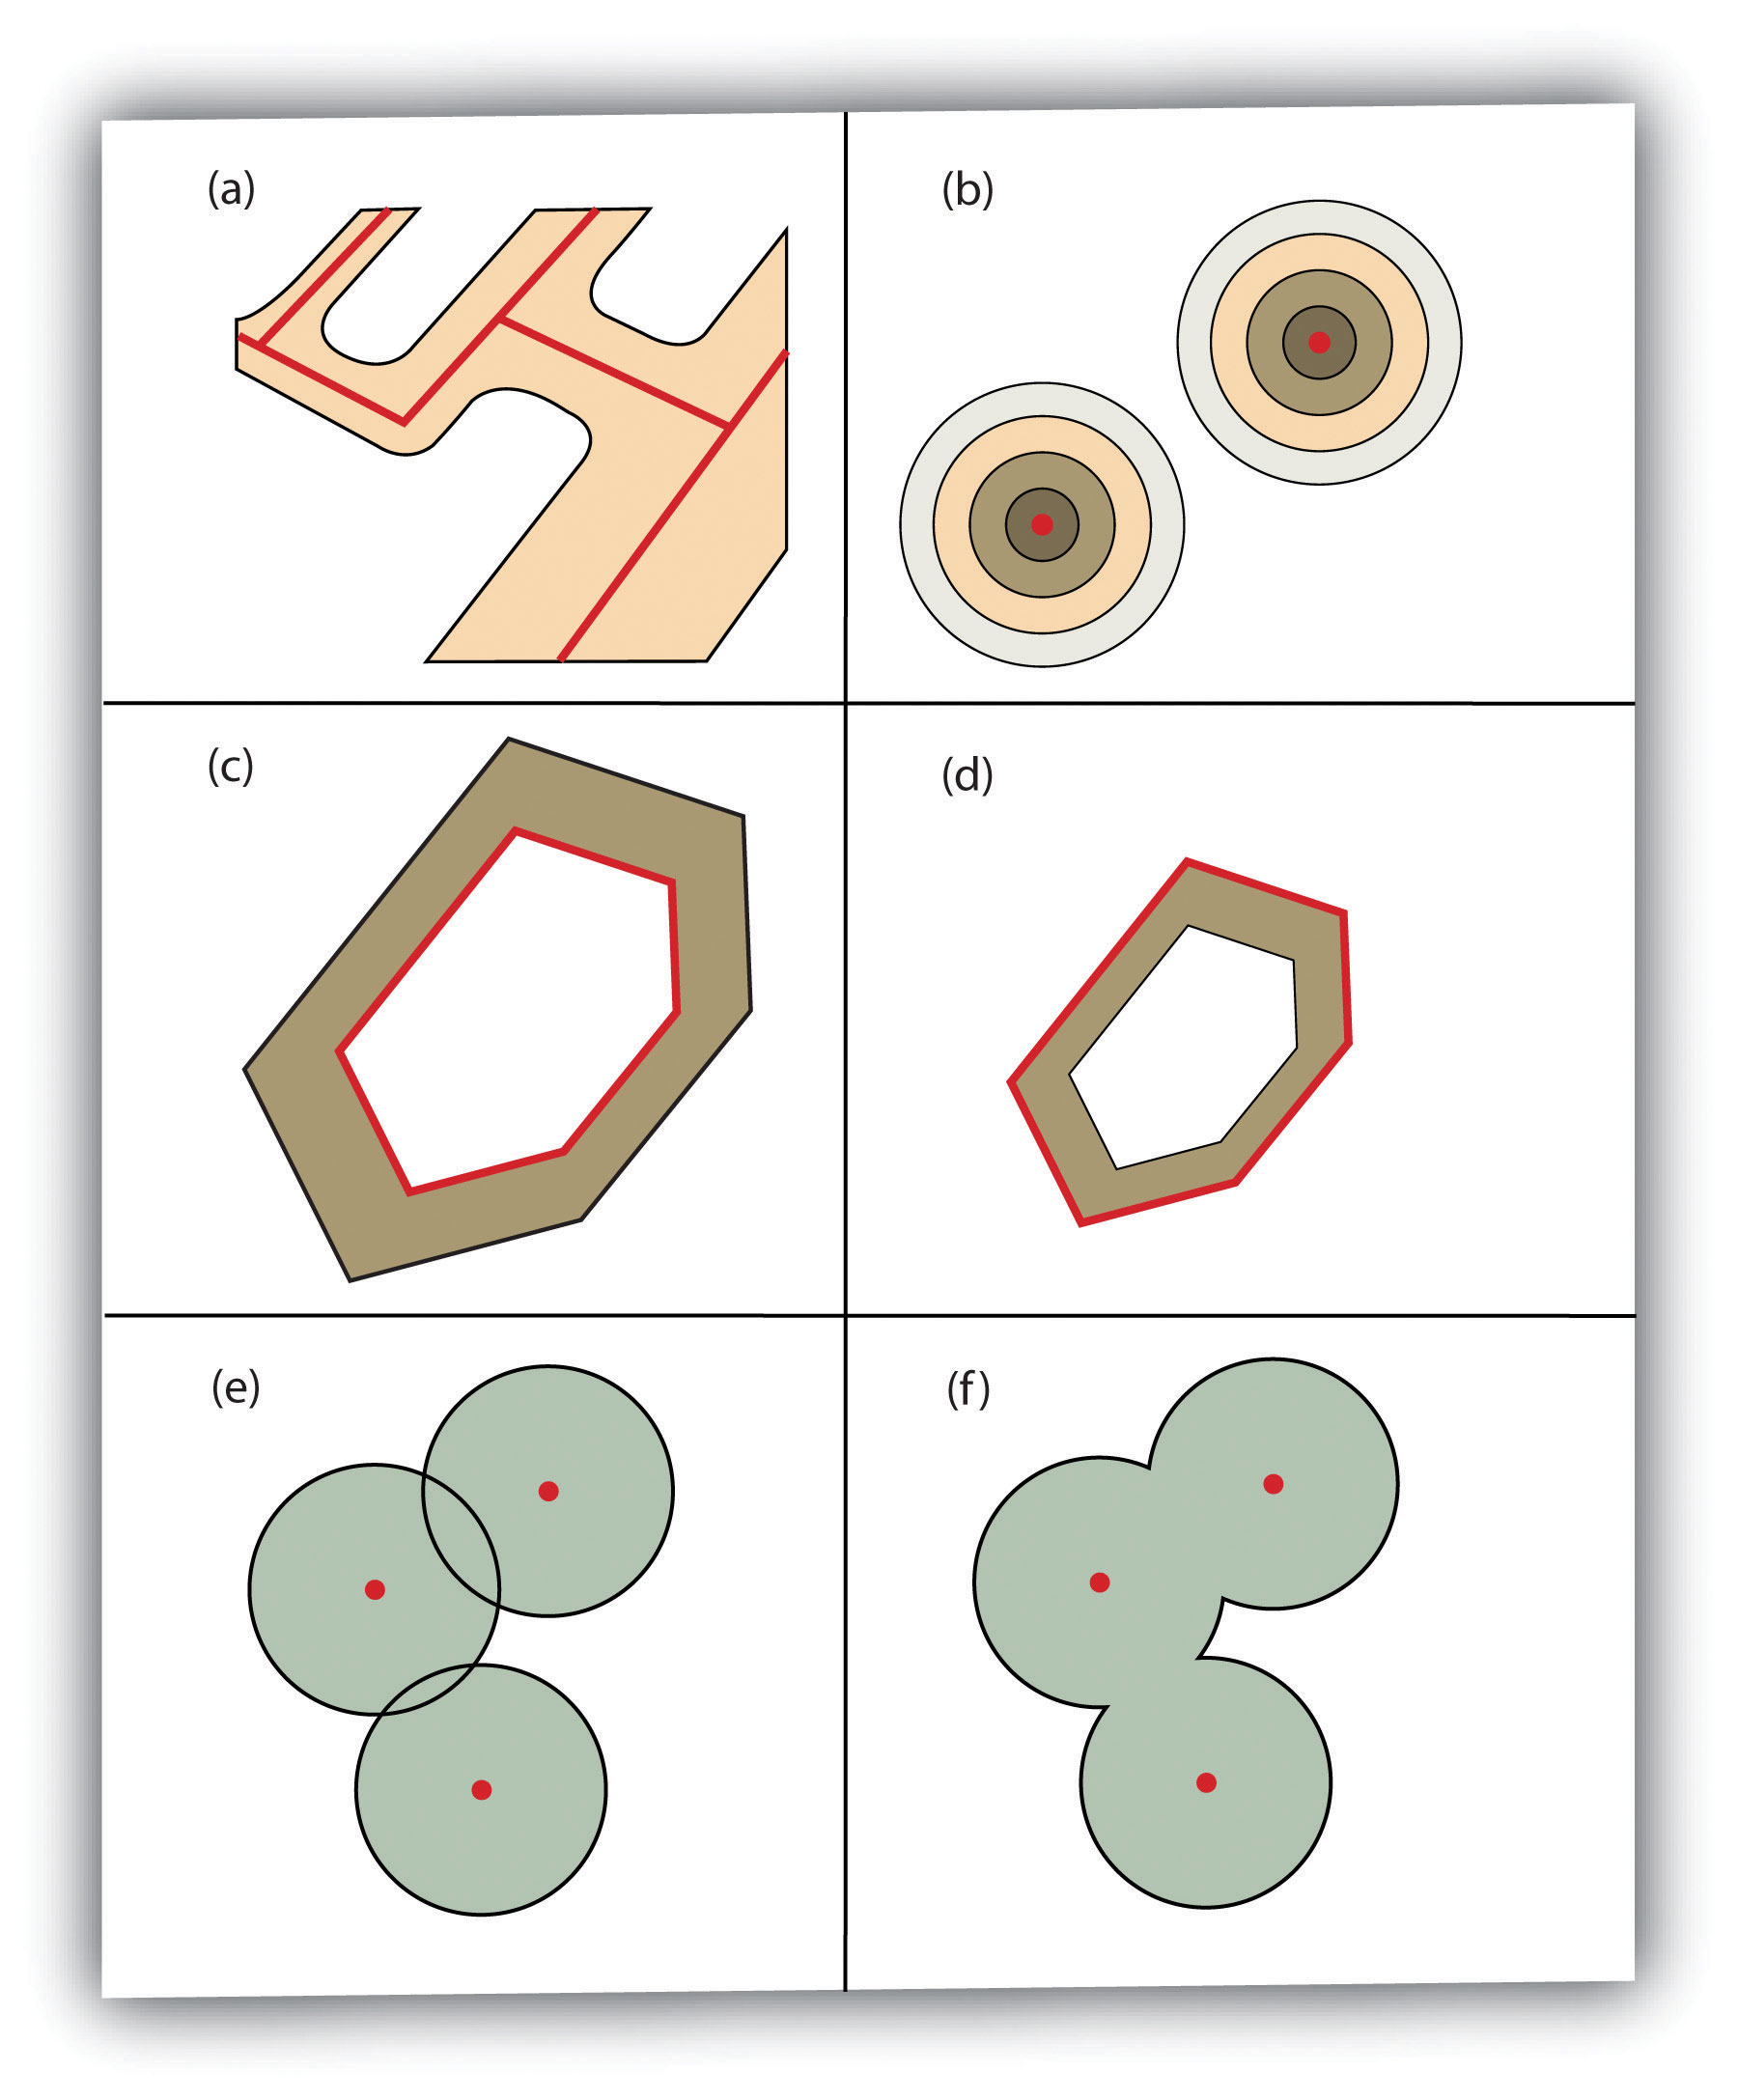
\includegraphics[width=1\linewidth]{img/buffer_operations} \caption{Buffer Options: (a) Variable Width Buffers, (b) Multiple Ring Buffers, (c) Doughnut Buffer, (d) Setback Buffer, (e) Nondissolved Buffer, (f) Dissolved Buffer}\label{fig:buffer-types}
\end{figure}

\begin{figure}
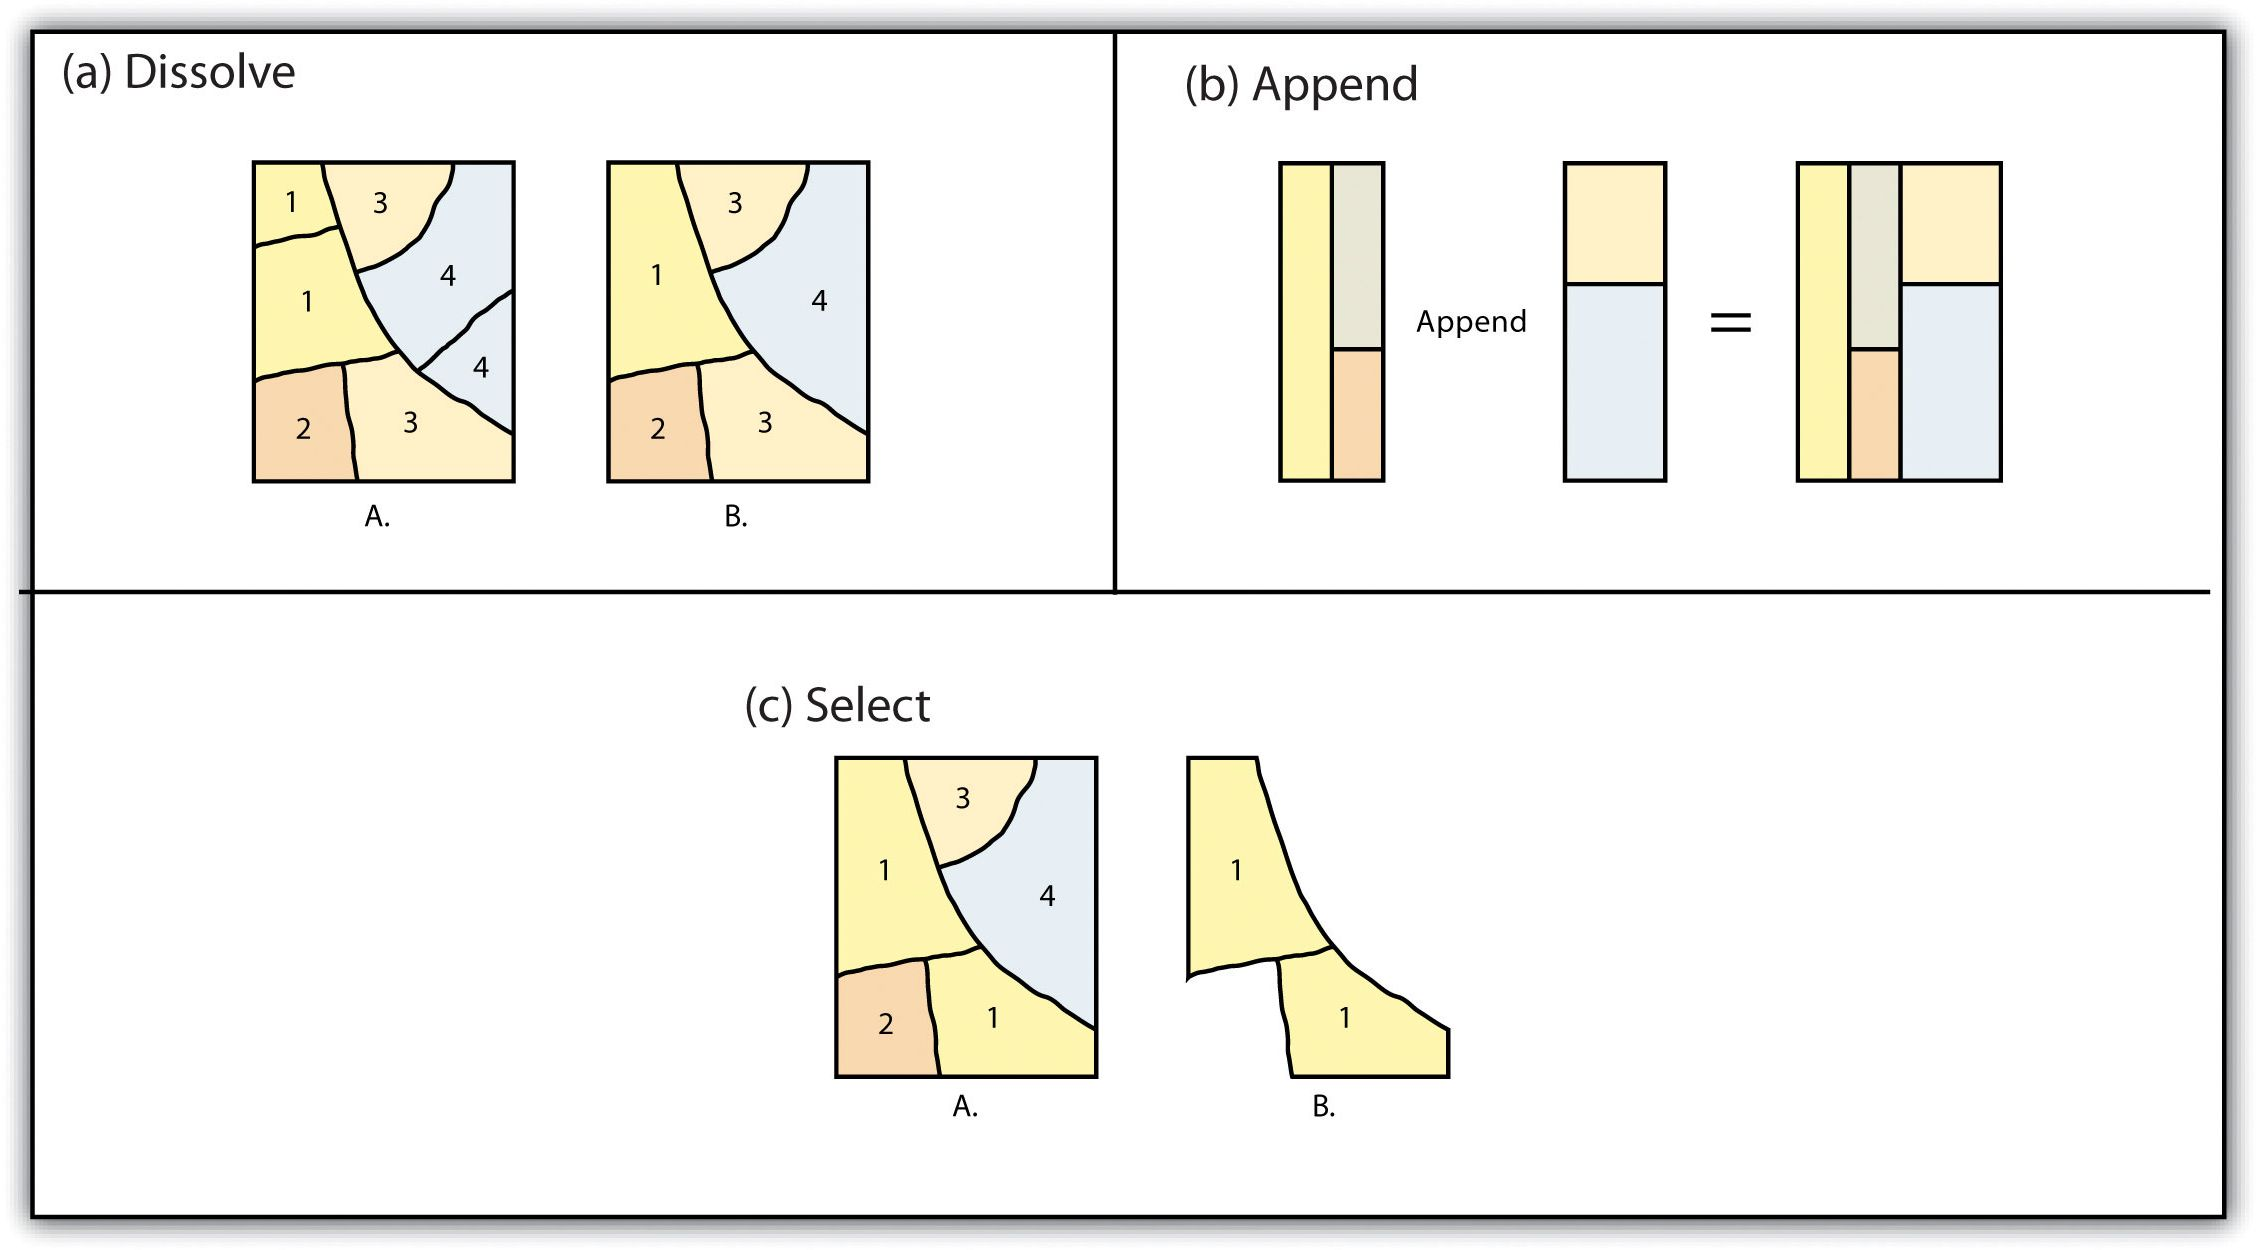
\includegraphics[width=1\linewidth]{img/single_layer_operation} \caption{Single Layer Geometric Operations}\label{fig:single-layer-ops}
\end{figure}

\begin{figure}
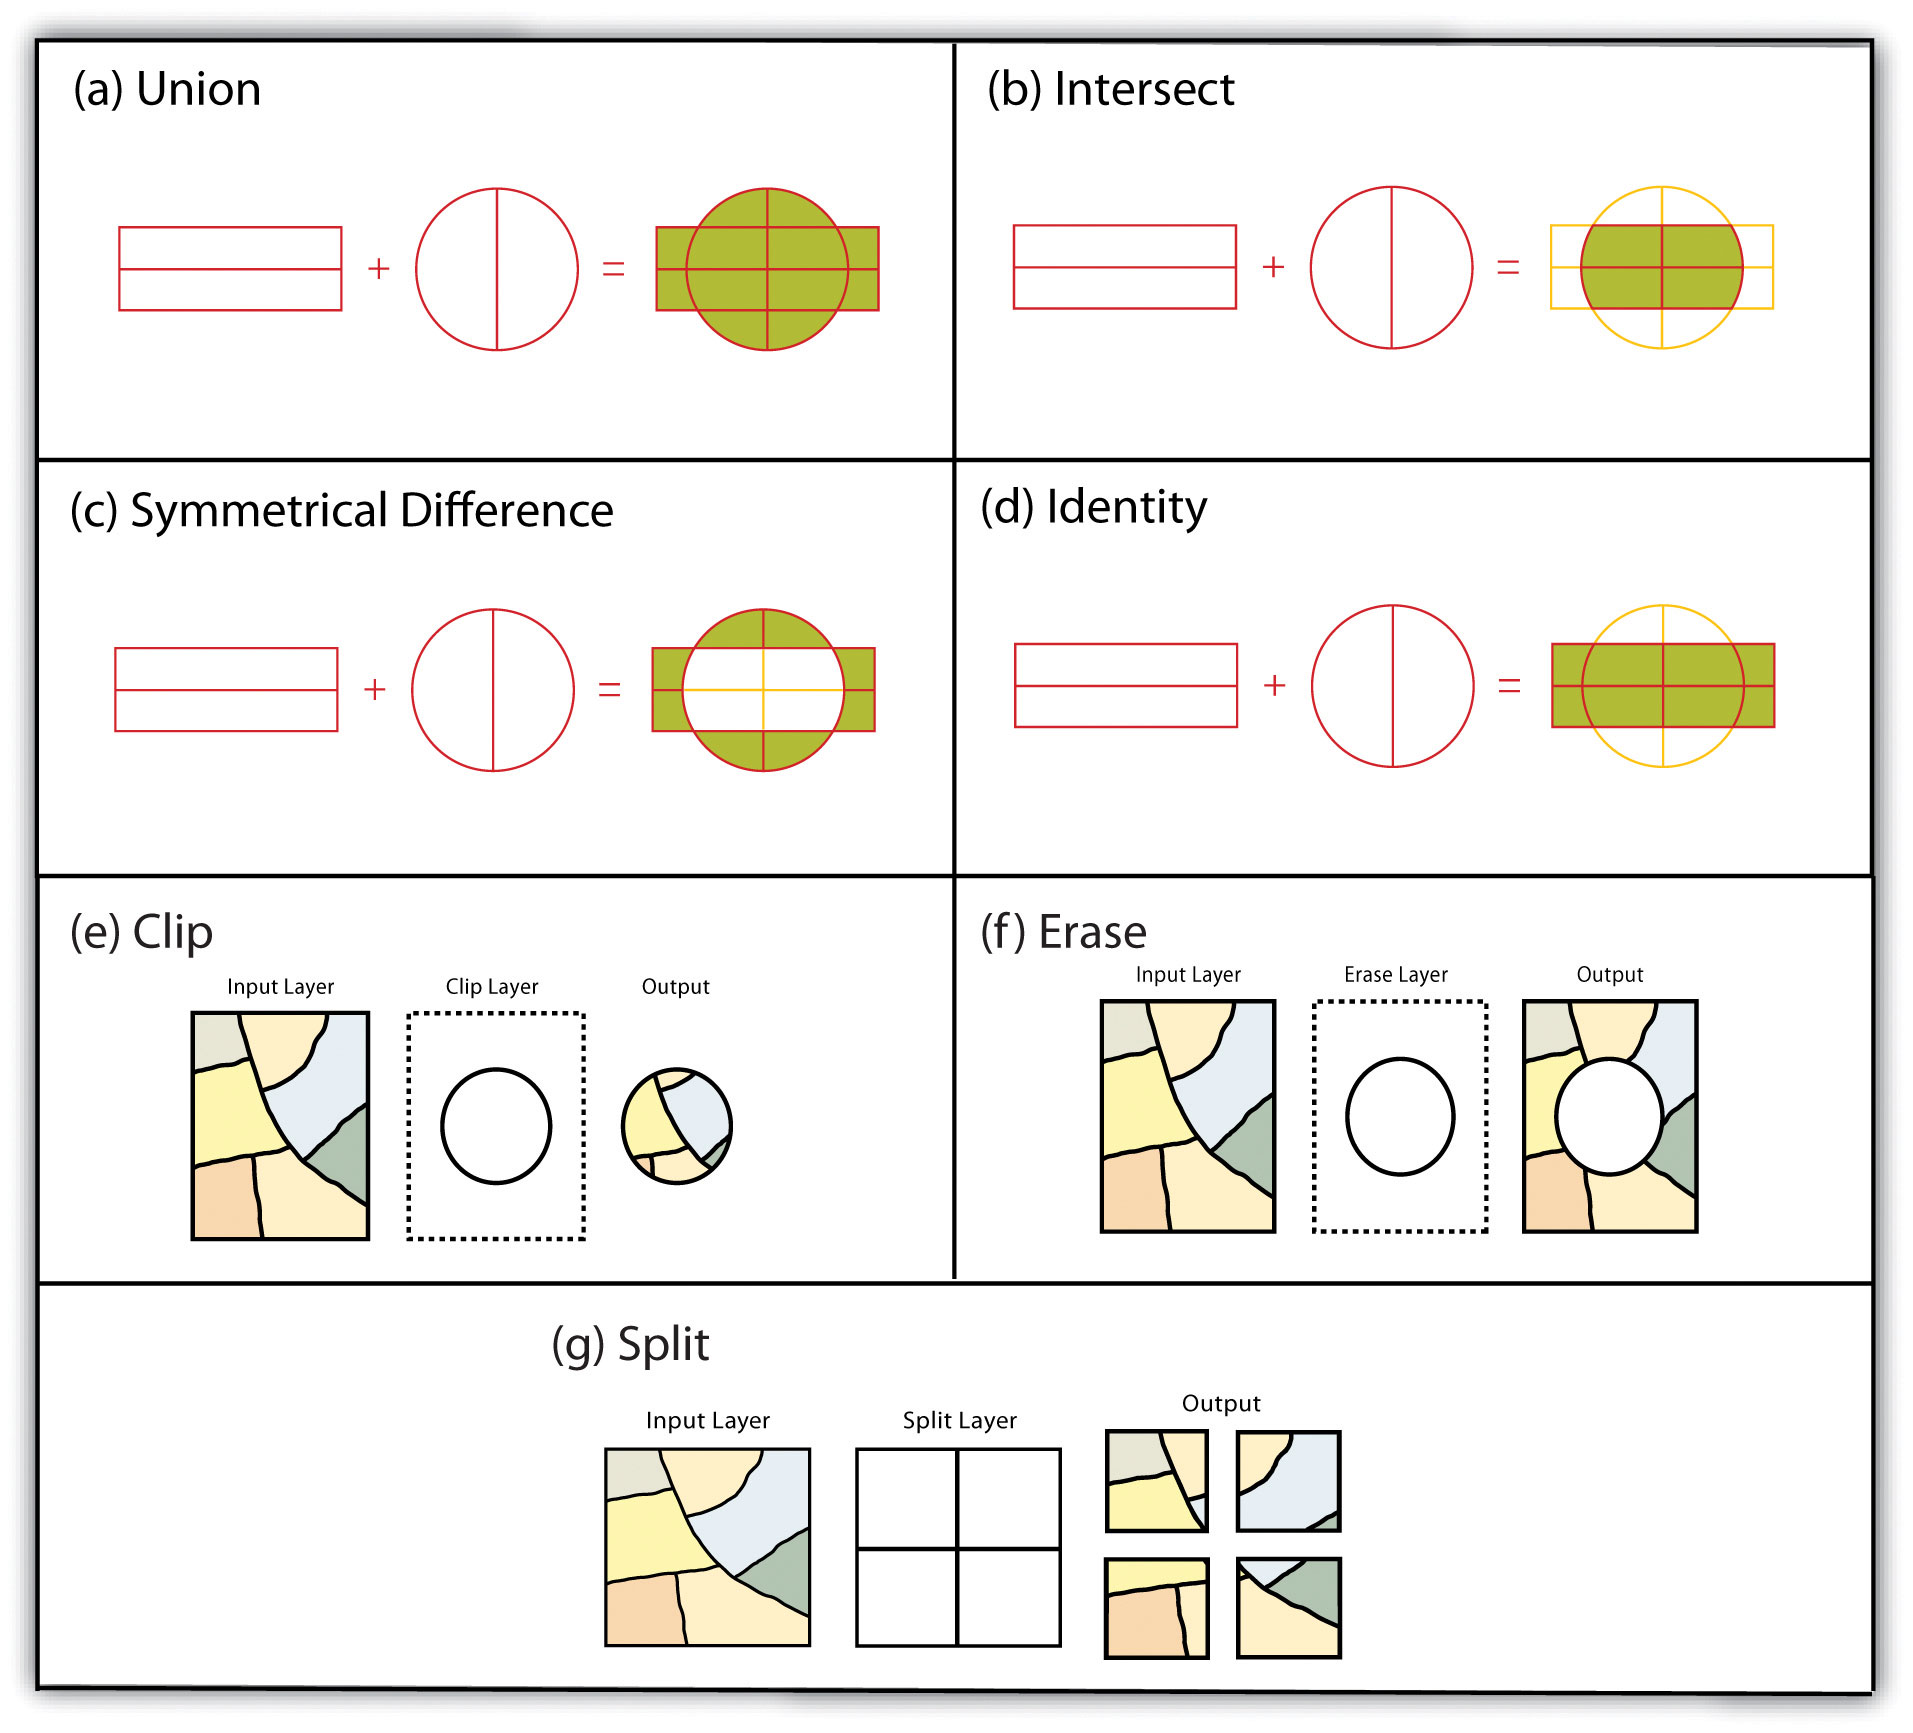
\includegraphics[width=1\linewidth]{img/multi-layer-overlay} \caption{Multiple Layer Geometric Operations}\label{fig:multi-layer-ops}
\end{figure}

\begin{quote}
\textbf{\emph{Self Exercise}}

\begin{itemize}
\tightlist
\item
  Think about how to conduct these spatial operations using basic \textbf{\emph{sf}} st\_ and tidyverse functions.
\item
  Dissolve: merge (data.frame), dplyr::group\_by, st\_union
\item
  Append: dplyr::bind\_rows, st\_combine (may not give you what you expect, though)
\item
  Identity: st\_union and then st\_intersection
\item
  Erase: st\_difference
\item
  Split: st\_intersection by feature ID
\end{itemize}
\end{quote}

Geometric operations are algorithmically difficult and computationally expensive. So, quite often, results are not what we expected. More mature packages perform better. In this case, sp-family packages are better than sf-family.

\begin{Shaded}
\begin{Highlighting}[]
\NormalTok{buf\_sf }\OtherTok{\textless{}{-}}\NormalTok{  hunter\_college\_sf }\SpecialCharTok{\%\textgreater{}\%}\NormalTok{ sf}\SpecialCharTok{::}\FunctionTok{st\_transform}\NormalTok{(}\DecValTok{2831}\NormalTok{) }\SpecialCharTok{\%\textgreater{}\%} \CommentTok{\# reproject the data to 2831}
\NormalTok{    sf}\SpecialCharTok{::}\FunctionTok{st\_buffer}\NormalTok{(}\DecValTok{800}\NormalTok{) }\CommentTok{\# create the buffer}

\NormalTok{man\_tracts\_sf }\OtherTok{\textless{}{-}}\NormalTok{ nyc\_census\_tracts\_sf }\SpecialCharTok{\%\textgreater{}\%} 
  \FunctionTok{st\_transform}\NormalTok{(}\DecValTok{2831}\NormalTok{) }\SpecialCharTok{\%\textgreater{}\%}
  \FunctionTok{filter}\NormalTok{(COUNTYFP }\SpecialCharTok{==} \StringTok{\textquotesingle{}061\textquotesingle{}}\NormalTok{)}

\NormalTok{buf\_sel\_sf }\OtherTok{\textless{}{-}}\NormalTok{ buf\_sf }\SpecialCharTok{\%\textgreater{}\%} 
\NormalTok{    sf}\SpecialCharTok{::}\FunctionTok{st\_intersects}\NormalTok{(man\_tracts\_sf) }\SpecialCharTok{\%\textgreater{}\%} \CommentTok{\# intersects with the transformed noise data}
\NormalTok{    magrittr}\SpecialCharTok{::}\FunctionTok{extract2}\NormalTok{(., }\DecValTok{1}\NormalTok{) }\SpecialCharTok{\%\textgreater{}\%} \CommentTok{\# Get the indices of the noise points within 200 meter buffer}
\NormalTok{    dplyr}\SpecialCharTok{::}\FunctionTok{slice}\NormalTok{(man\_tracts\_sf, .) }

\FunctionTok{par}\NormalTok{(}\AttributeTok{mfrow=}\FunctionTok{c}\NormalTok{(}\DecValTok{1}\NormalTok{,}\DecValTok{2}\NormalTok{), }\AttributeTok{mar =} \FunctionTok{c}\NormalTok{(}\DecValTok{4}\NormalTok{, }\FloatTok{0.1}\NormalTok{, }\FloatTok{0.8}\NormalTok{, }\FloatTok{0.1}\NormalTok{))}

\FunctionTok{plot}\NormalTok{(buf\_sf }\SpecialCharTok{\%\textgreater{}\%} \FunctionTok{st\_geometry}\NormalTok{(), }
     \AttributeTok{col=}\StringTok{\textquotesingle{}grey\textquotesingle{}}\NormalTok{, }
     \AttributeTok{main =} \StringTok{\textquotesingle{}Buffer Geometry\textquotesingle{}}\NormalTok{)}

\FunctionTok{plot}\NormalTok{(buf\_sel\_sf  }\SpecialCharTok{\%\textgreater{}\%} \FunctionTok{st\_geometry}\NormalTok{(), }
     \AttributeTok{col=}\StringTok{\textquotesingle{}lightskyblue2\textquotesingle{}}\NormalTok{, }
     \AttributeTok{main=}\StringTok{"Polygons"}\NormalTok{)}
\end{Highlighting}
\end{Shaded}

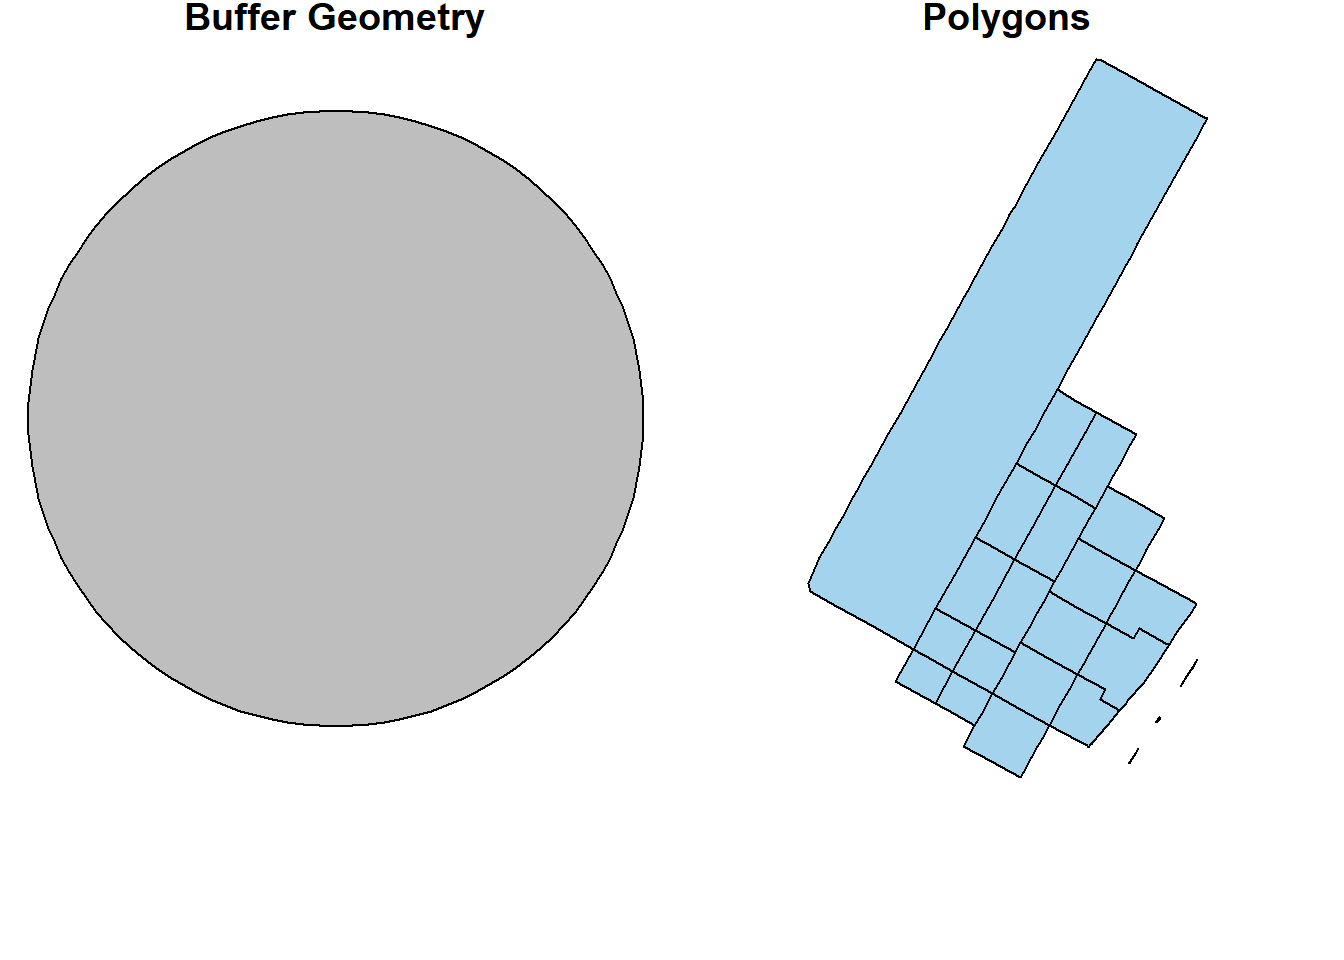
\includegraphics[width=0.9\linewidth]{R-spatial_files/figure-latex/geomOperations-1}

\begin{Shaded}
\begin{Highlighting}[]
\FunctionTok{st\_union}\NormalTok{(buf\_sel\_sf, buf\_sf,}\AttributeTok{by\_feature =} \ConstantTok{TRUE}\NormalTok{) }\SpecialCharTok{\%\textgreater{}\%} 
  \FunctionTok{st\_geometry}\NormalTok{() }\SpecialCharTok{\%\textgreater{}\%} 
  \FunctionTok{plot}\NormalTok{(}\AttributeTok{col=}\StringTok{\textquotesingle{}lightskyblue1\textquotesingle{}}\NormalTok{, }\AttributeTok{main =} \StringTok{\textquotesingle{}sf::st\_union by feature\textquotesingle{}}\NormalTok{)}

\NormalTok{rgeos}\SpecialCharTok{::}\FunctionTok{gUnion}\NormalTok{(buf\_sf }\SpecialCharTok{\%\textgreater{}\%}\NormalTok{ sf}\SpecialCharTok{::}\FunctionTok{as\_Spatial}\NormalTok{(), }
\NormalTok{              buf\_sel\_sf }\SpecialCharTok{\%\textgreater{}\%}\NormalTok{ sf}\SpecialCharTok{::}\FunctionTok{as\_Spatial}\NormalTok{(), }
              \AttributeTok{byid =} \ConstantTok{TRUE}\NormalTok{) }\SpecialCharTok{\%\textgreater{}\%} 
  \FunctionTok{plot}\NormalTok{(}\AttributeTok{col=}\StringTok{\textquotesingle{}lightpink\textquotesingle{}}\NormalTok{, }\AttributeTok{main =} \StringTok{\textquotesingle{}rgeos::gUnion (sp) by feature\textquotesingle{}}\NormalTok{)}
\end{Highlighting}
\end{Shaded}

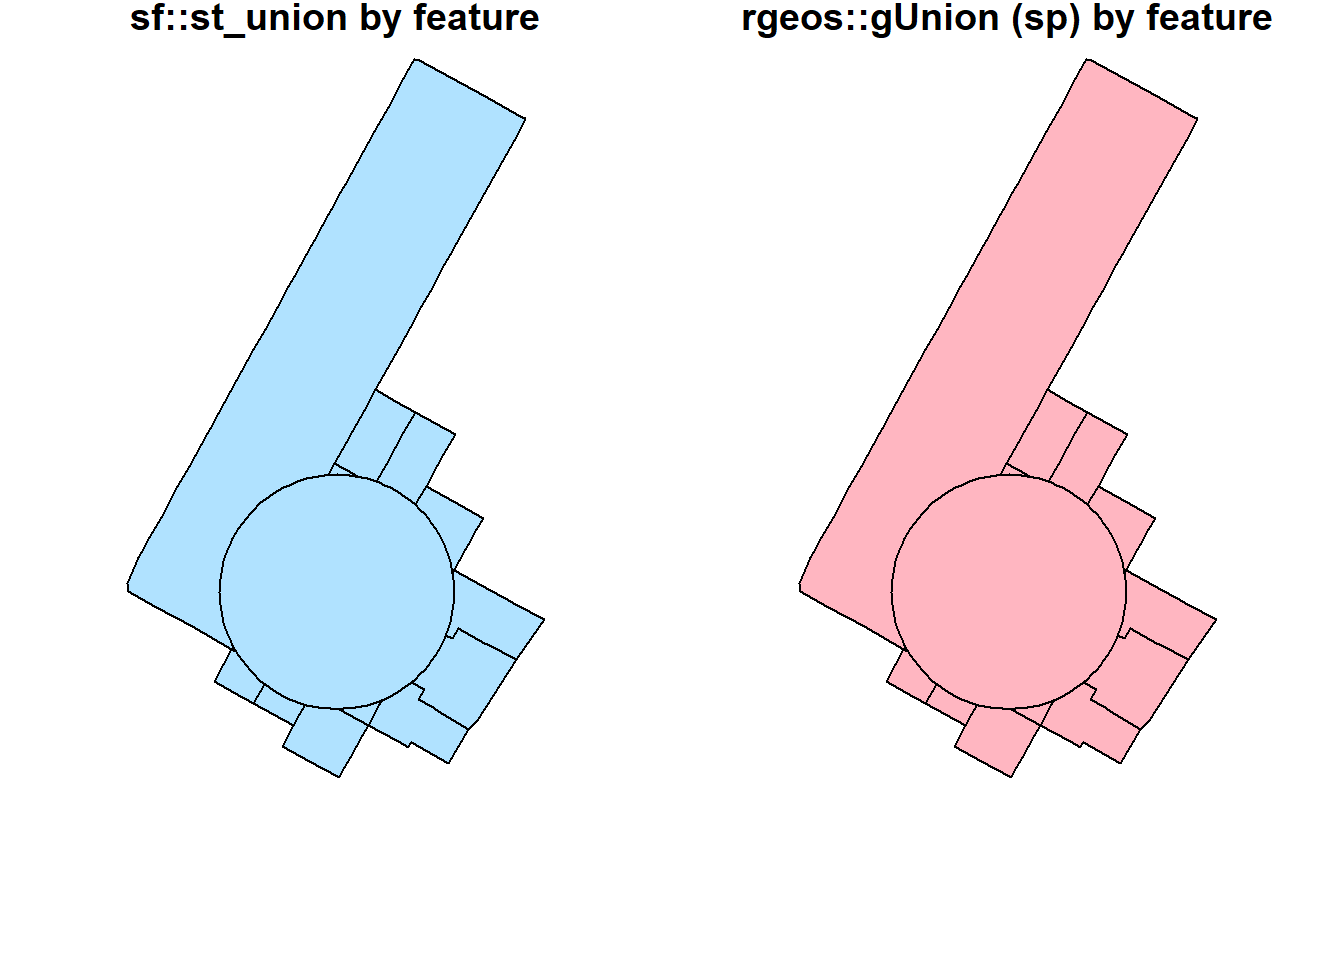
\includegraphics[width=0.9\linewidth]{R-spatial_files/figure-latex/geomOperations-2}

\begin{Shaded}
\begin{Highlighting}[]
\FunctionTok{st\_union}\NormalTok{(buf\_sel\_sf, buf\_sf,}\AttributeTok{by\_feature =} \ConstantTok{FALSE}\NormalTok{) }\SpecialCharTok{\%\textgreater{}\%} 
  \FunctionTok{st\_geometry}\NormalTok{() }\SpecialCharTok{\%\textgreater{}\%} 
  \FunctionTok{plot}\NormalTok{(}\AttributeTok{col=}\StringTok{\textquotesingle{}lightskyblue1\textquotesingle{}}\NormalTok{, }\AttributeTok{main =} \StringTok{\textquotesingle{}sf::st\_union\textquotesingle{}}\NormalTok{)}

\NormalTok{rgeos}\SpecialCharTok{::}\FunctionTok{gUnion}\NormalTok{(buf\_sf }\SpecialCharTok{\%\textgreater{}\%}\NormalTok{ sf}\SpecialCharTok{::}\FunctionTok{as\_Spatial}\NormalTok{(), }
\NormalTok{              buf\_sel\_sf }\SpecialCharTok{\%\textgreater{}\%}\NormalTok{ sf}\SpecialCharTok{::}\FunctionTok{as\_Spatial}\NormalTok{()) }\SpecialCharTok{\%\textgreater{}\%} 
  \FunctionTok{plot}\NormalTok{(}\AttributeTok{col=}\StringTok{\textquotesingle{}lightpink\textquotesingle{}}\NormalTok{, }\AttributeTok{main =} \StringTok{\textquotesingle{}rgeos::gUnion (sp)\textquotesingle{}}\NormalTok{)}
\end{Highlighting}
\end{Shaded}

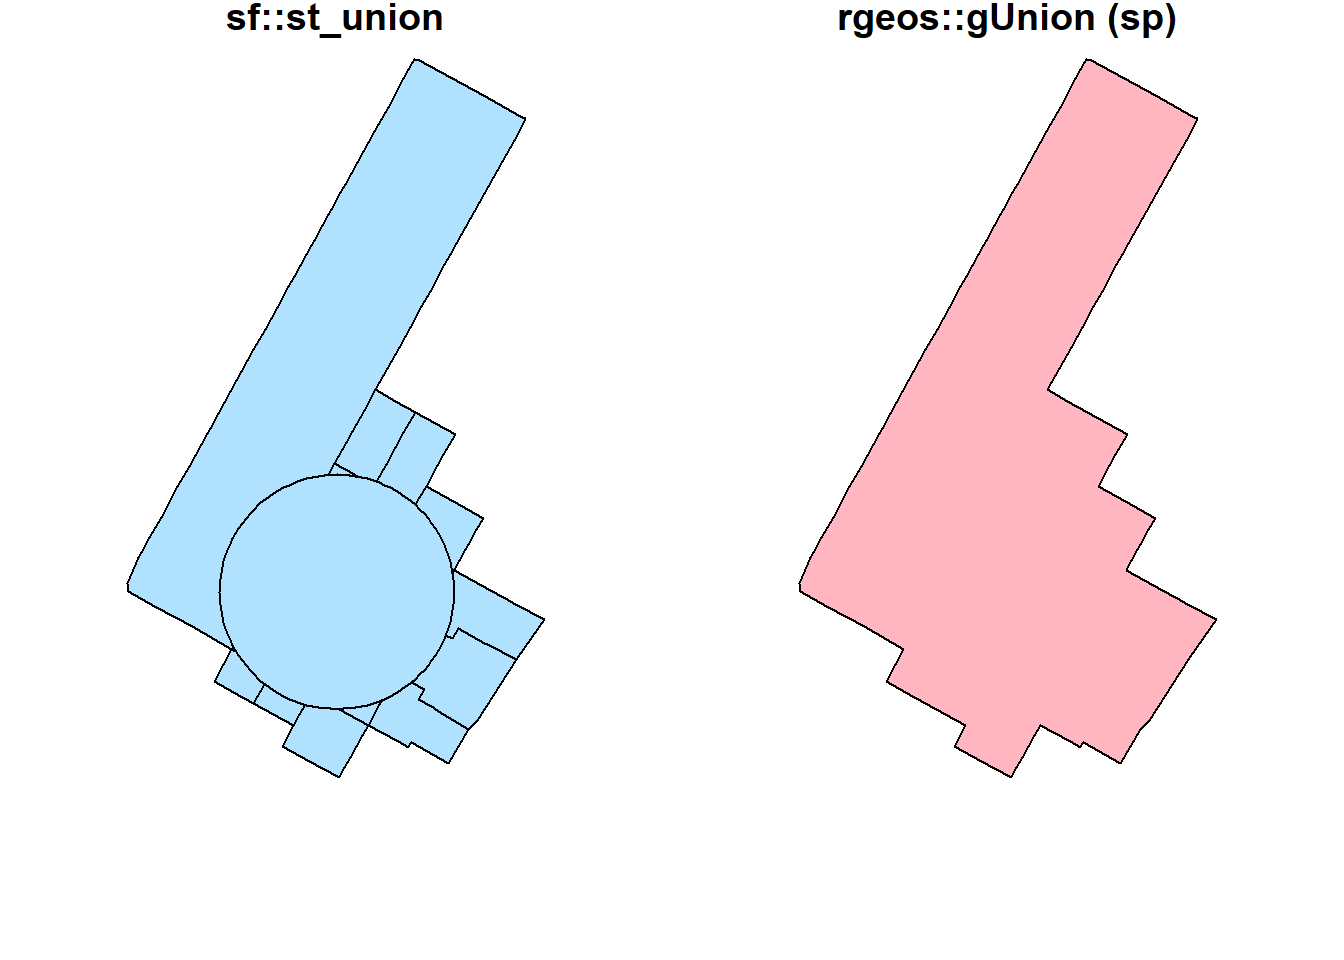
\includegraphics[width=0.9\linewidth]{R-spatial_files/figure-latex/geomOperations-3}

\begin{Shaded}
\begin{Highlighting}[]
\FunctionTok{st\_intersection}\NormalTok{(buf\_sel\_sf, buf\_sf) }\SpecialCharTok{\%\textgreater{}\%} 
  \FunctionTok{st\_geometry}\NormalTok{() }\SpecialCharTok{\%\textgreater{}\%} 
  \FunctionTok{plot}\NormalTok{(}\AttributeTok{col=}\StringTok{\textquotesingle{}lightskyblue1\textquotesingle{}}\NormalTok{, }\AttributeTok{main =} \StringTok{\textquotesingle{}sf::st\_intersection\textquotesingle{}}\NormalTok{)}

\FunctionTok{st\_difference}\NormalTok{(buf\_sel\_sf, buf\_sf) }\SpecialCharTok{\%\textgreater{}\%} \FunctionTok{st\_geometry}\NormalTok{() }\SpecialCharTok{\%\textgreater{}\%} 
  \FunctionTok{plot}\NormalTok{(}\AttributeTok{col=}\StringTok{\textquotesingle{}lightskyblue1\textquotesingle{}}\NormalTok{,}\AttributeTok{main =} \StringTok{\textquotesingle{}sf::st\_difference\textquotesingle{}}\NormalTok{)}
\end{Highlighting}
\end{Shaded}

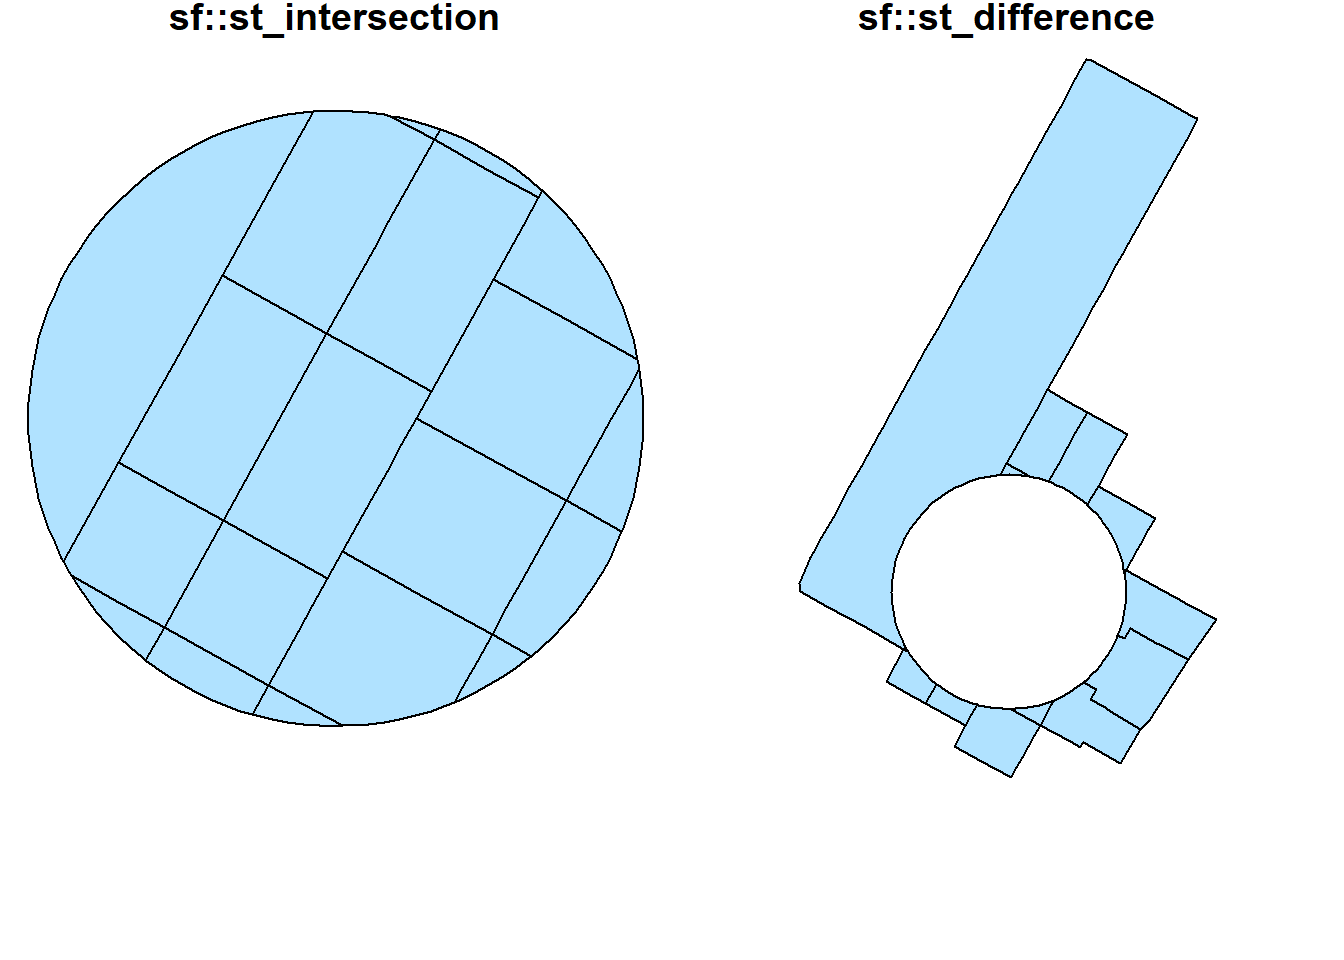
\includegraphics[width=0.9\linewidth]{R-spatial_files/figure-latex/geomOperations-4}

\begin{Shaded}
\begin{Highlighting}[]
\FunctionTok{st\_sym\_difference}\NormalTok{(buf\_sel\_sf, buf\_sf) }\SpecialCharTok{\%\textgreater{}\%} 
  \FunctionTok{st\_geometry}\NormalTok{() }\SpecialCharTok{\%\textgreater{}\%} 
  \FunctionTok{plot}\NormalTok{(}\AttributeTok{col=}\StringTok{\textquotesingle{}lightskyblue1\textquotesingle{}}\NormalTok{,}\AttributeTok{main =} \StringTok{\textquotesingle{}sf::st\_sym\_difference\textquotesingle{}}\NormalTok{)}

\NormalTok{rgeos}\SpecialCharTok{::}\FunctionTok{gSymdifference}\NormalTok{(buf\_sf }\SpecialCharTok{\%\textgreater{}\%}\NormalTok{ sf}\SpecialCharTok{::}\FunctionTok{as\_Spatial}\NormalTok{(), }
\NormalTok{                      buf\_sel\_sf }\SpecialCharTok{\%\textgreater{}\%}\NormalTok{ sf}\SpecialCharTok{::}\FunctionTok{as\_Spatial}\NormalTok{(), }
                      \AttributeTok{drop\_lower\_td =} \ConstantTok{TRUE}\NormalTok{) }\SpecialCharTok{\%\textgreater{}\%} 
  \FunctionTok{plot}\NormalTok{(}\AttributeTok{col=}\StringTok{\textquotesingle{}lightpink\textquotesingle{}}\NormalTok{, }\AttributeTok{main =} \StringTok{\textquotesingle{}rgeos::gSymdifference (sp)\textquotesingle{}}\NormalTok{)}
\end{Highlighting}
\end{Shaded}

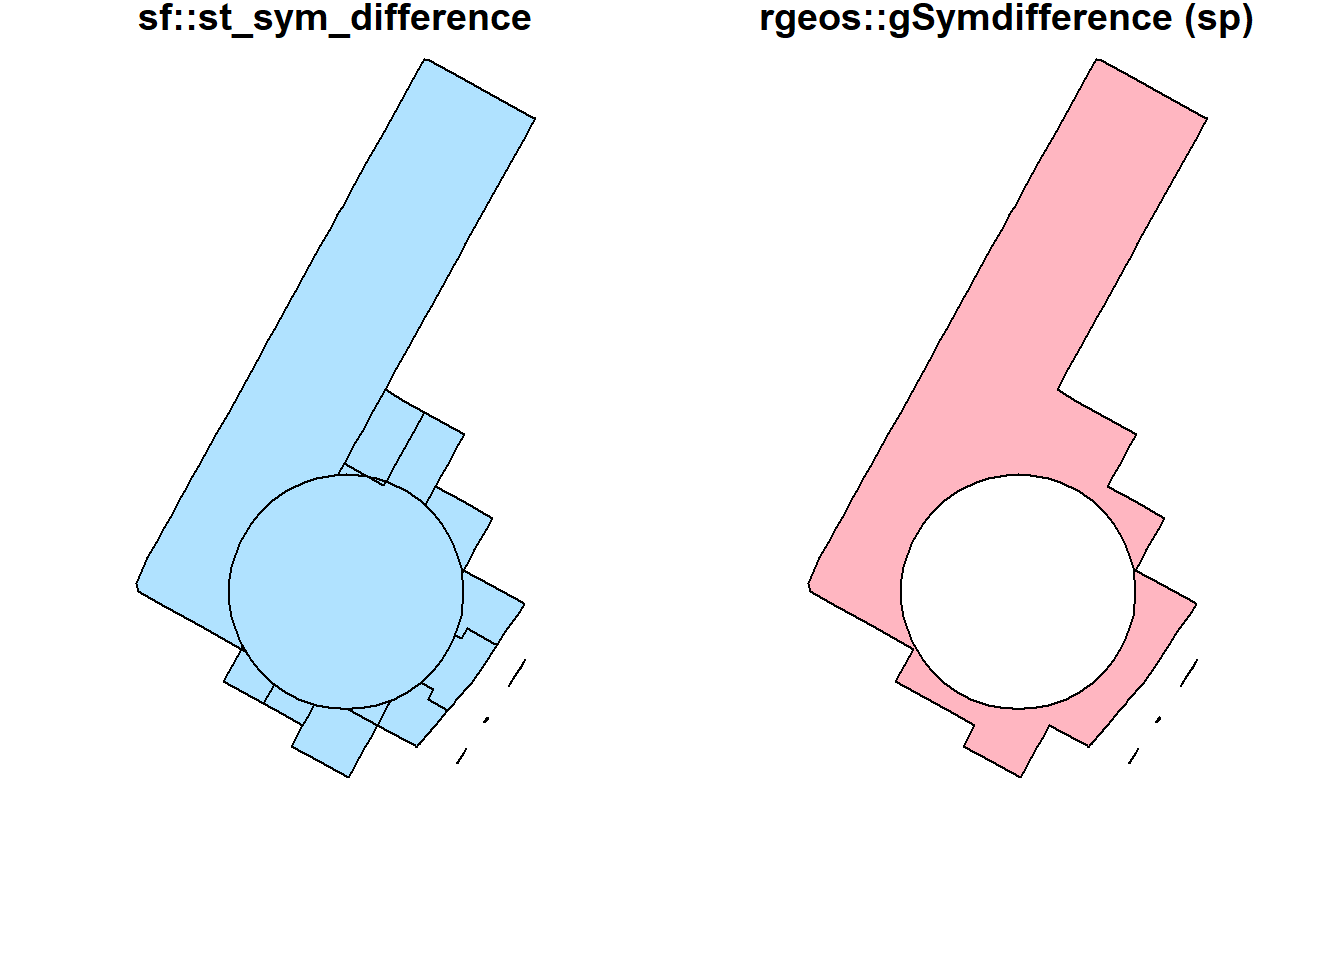
\includegraphics[width=0.9\linewidth]{R-spatial_files/figure-latex/geomOperations-5}

Interestingly, the \textbf{\emph{raster}} package seems to have better \emph{intersect} and \emph{union} methods. Results from these methods are similar to what popular GIS software like ArcGIS produces. More importantly, they keep all the attributes from both layers.

\begin{Shaded}
\begin{Highlighting}[]
\FunctionTok{par}\NormalTok{(}\AttributeTok{mfrow=}\FunctionTok{c}\NormalTok{(}\DecValTok{1}\NormalTok{,}\DecValTok{2}\NormalTok{), }\AttributeTok{mar =} \FunctionTok{c}\NormalTok{(}\DecValTok{4}\NormalTok{, }\FloatTok{0.1}\NormalTok{, }\FloatTok{0.8}\NormalTok{, }\FloatTok{0.1}\NormalTok{));}
\NormalTok{raster}\SpecialCharTok{::}\FunctionTok{union}\NormalTok{(buf\_sf }\SpecialCharTok{\%\textgreater{}\%}\NormalTok{ sf}\SpecialCharTok{::}\FunctionTok{st\_geometry}\NormalTok{() }\SpecialCharTok{\%\textgreater{}\%}\NormalTok{ sf}\SpecialCharTok{::}\FunctionTok{as\_Spatial}\NormalTok{(),}
\NormalTok{              buf\_sel\_sf }\SpecialCharTok{\%\textgreater{}\%}\NormalTok{ sf}\SpecialCharTok{::}\FunctionTok{st\_geometry}\NormalTok{() }\SpecialCharTok{\%\textgreater{}\%}\NormalTok{ sf}\SpecialCharTok{::}\FunctionTok{as\_Spatial}\NormalTok{()) }\SpecialCharTok{\%\textgreater{}\%} 
  \FunctionTok{plot}\NormalTok{(}\AttributeTok{col=}\StringTok{\textquotesingle{}lightpink\textquotesingle{}}\NormalTok{, }\AttributeTok{main =} \StringTok{\textquotesingle{}raster::union\textquotesingle{}}\NormalTok{);}

\NormalTok{raster}\SpecialCharTok{::}\FunctionTok{intersect}\NormalTok{(buf\_sf }\SpecialCharTok{\%\textgreater{}\%}\NormalTok{ sf}\SpecialCharTok{::}\FunctionTok{st\_geometry}\NormalTok{() }\SpecialCharTok{\%\textgreater{}\%}\NormalTok{ sf}\SpecialCharTok{::}\FunctionTok{as\_Spatial}\NormalTok{(), }
\NormalTok{                  buf\_sel\_sf }\SpecialCharTok{\%\textgreater{}\%}\NormalTok{ sf}\SpecialCharTok{::}\FunctionTok{st\_geometry}\NormalTok{() }\SpecialCharTok{\%\textgreater{}\%}\NormalTok{ sf}\SpecialCharTok{::}\FunctionTok{as\_Spatial}\NormalTok{()) }\SpecialCharTok{\%\textgreater{}\%} 
  \FunctionTok{plot}\NormalTok{(}\AttributeTok{col=}\StringTok{\textquotesingle{}lightpink\textquotesingle{}}\NormalTok{, }\AttributeTok{main =} \StringTok{\textquotesingle{}raster::intersect\textquotesingle{}}\NormalTok{)}
\end{Highlighting}
\end{Shaded}

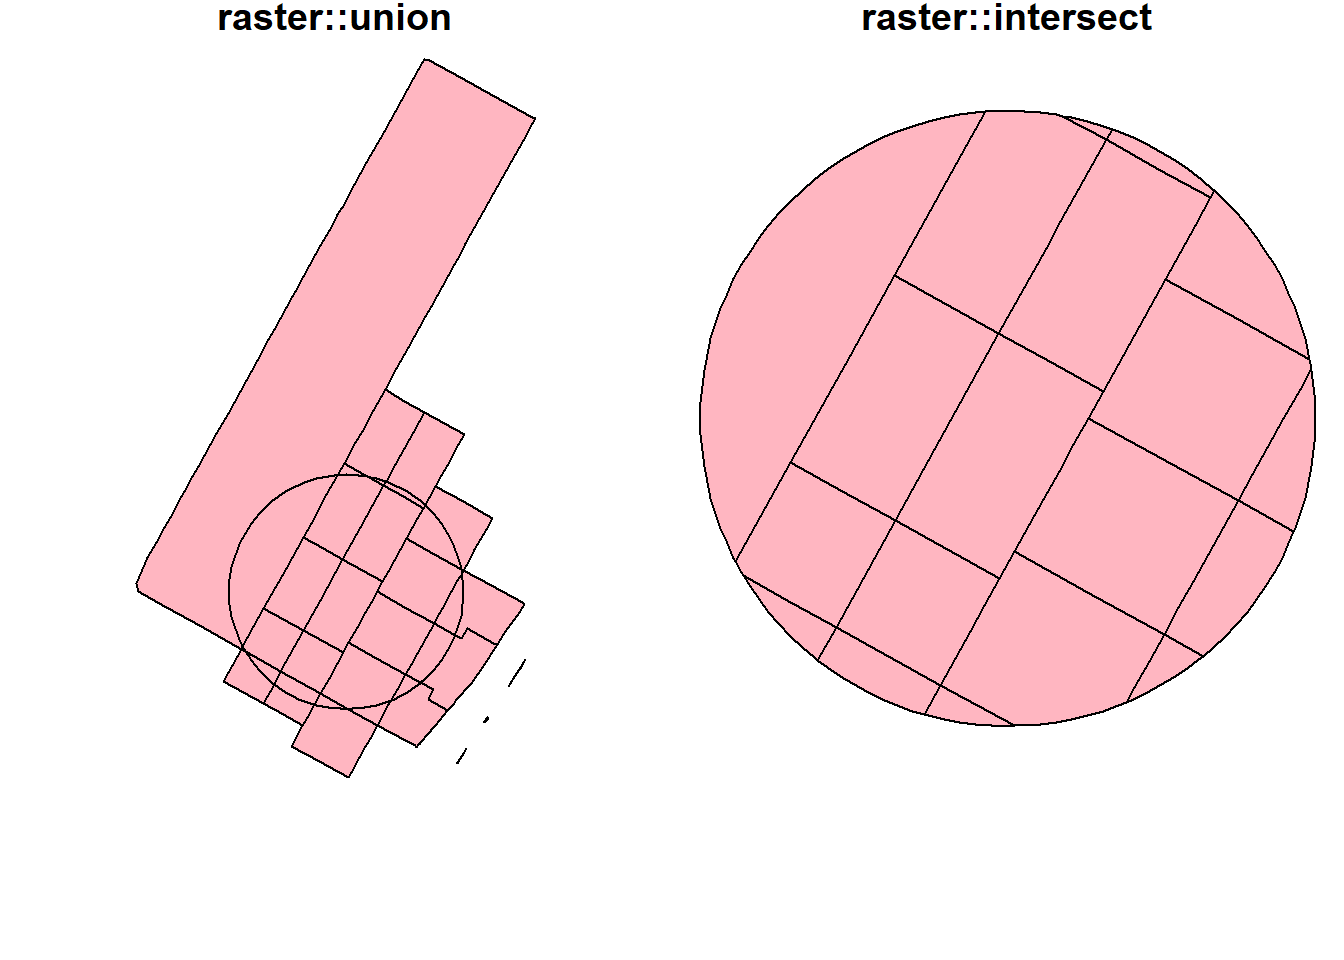
\includegraphics[width=0.9\linewidth]{R-spatial_files/figure-latex/geomOperationsRaster-1}

To visualize all these different operations with the orginal dataset.

\begin{Shaded}
\begin{Highlighting}[]
\CommentTok{\# Various types of spatial operations}
\FunctionTok{par}\NormalTok{(}\AttributeTok{mfrow=}\FunctionTok{c}\NormalTok{(}\DecValTok{1}\NormalTok{,}\DecValTok{2}\NormalTok{), }\AttributeTok{mar =} \FunctionTok{c}\NormalTok{(}\DecValTok{4}\NormalTok{, }\FloatTok{0.1}\NormalTok{, }\FloatTok{0.8}\NormalTok{, }\FloatTok{0.1}\NormalTok{))}

\FunctionTok{plot}\NormalTok{(}\FunctionTok{st\_geometry}\NormalTok{(man\_tracts\_sf), }\AttributeTok{border=}\StringTok{"\#aaaaaa"}\NormalTok{, }\AttributeTok{main=}\StringTok{"Buffer Geometry"}\NormalTok{)}
\FunctionTok{plot}\NormalTok{(buf\_sf }\SpecialCharTok{\%\textgreater{}\%} \FunctionTok{st\_geometry}\NormalTok{(), }
     \AttributeTok{col=}\StringTok{\textquotesingle{}grey\textquotesingle{}}\NormalTok{, }
     \AttributeTok{add=}\NormalTok{T)}

\FunctionTok{plot}\NormalTok{(}\FunctionTok{st\_geometry}\NormalTok{(man\_tracts\_sf), }\AttributeTok{border=}\StringTok{"\#aaaaaa"}\NormalTok{, }\AttributeTok{main=}\StringTok{"Polygons"}\NormalTok{)}
\FunctionTok{plot}\NormalTok{(buf\_sel\_sf  }\SpecialCharTok{\%\textgreater{}\%} \FunctionTok{st\_geometry}\NormalTok{(), }
     \AttributeTok{col=}\StringTok{\textquotesingle{}lightskyblue2\textquotesingle{}}\NormalTok{, }
     \AttributeTok{add=}\NormalTok{T)}
\end{Highlighting}
\end{Shaded}

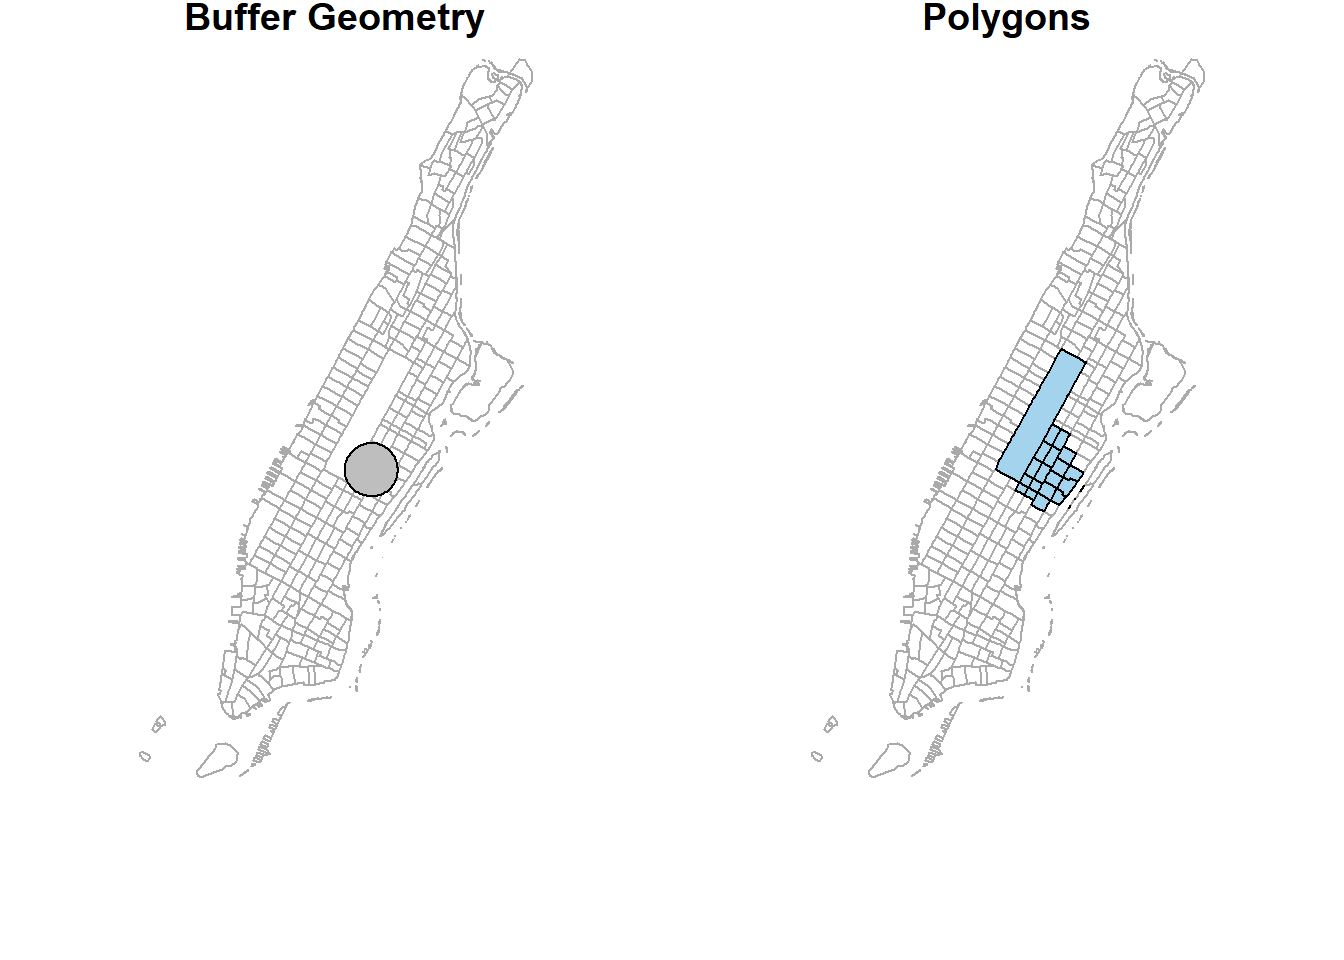
\includegraphics{R-spatial_files/figure-latex/geomOperationsBG-1.pdf}

\begin{Shaded}
\begin{Highlighting}[]
\FunctionTok{plot}\NormalTok{(}\FunctionTok{st\_geometry}\NormalTok{(man\_tracts\_sf), }\AttributeTok{border=}\StringTok{"\#aaaaaa"}\NormalTok{, }\AttributeTok{main=}\StringTok{"sf::st\_union by feature"}\NormalTok{)}
\FunctionTok{st\_union}\NormalTok{(buf\_sel\_sf, buf\_sf,}\AttributeTok{by\_feature =} \ConstantTok{TRUE}\NormalTok{) }\SpecialCharTok{\%\textgreater{}\%} 
  \FunctionTok{st\_geometry}\NormalTok{() }\SpecialCharTok{\%\textgreater{}\%} 
  \FunctionTok{plot}\NormalTok{(}\AttributeTok{col=}\StringTok{\textquotesingle{}lightskyblue1\textquotesingle{}}\NormalTok{, }\AttributeTok{add =}\NormalTok{ T)}

\FunctionTok{plot}\NormalTok{(}\FunctionTok{st\_geometry}\NormalTok{(man\_tracts\_sf), }\AttributeTok{border=}\StringTok{"\#aaaaaa"}\NormalTok{, }\AttributeTok{main=}\StringTok{\textquotesingle{}rgeos::gUnion (sp) by feature\textquotesingle{}}\NormalTok{)}
\NormalTok{rgeos}\SpecialCharTok{::}\FunctionTok{gUnion}\NormalTok{(buf\_sf }\SpecialCharTok{\%\textgreater{}\%}\NormalTok{ sf}\SpecialCharTok{::}\FunctionTok{as\_Spatial}\NormalTok{(), }
\NormalTok{              buf\_sel\_sf }\SpecialCharTok{\%\textgreater{}\%}\NormalTok{ sf}\SpecialCharTok{::}\FunctionTok{as\_Spatial}\NormalTok{(), }
              \AttributeTok{byid =} \ConstantTok{TRUE}\NormalTok{) }\SpecialCharTok{\%\textgreater{}\%} 
  \FunctionTok{plot}\NormalTok{(}\AttributeTok{col=}\StringTok{\textquotesingle{}lightpink\textquotesingle{}}\NormalTok{, }\AttributeTok{add =}\NormalTok{ T)}
\end{Highlighting}
\end{Shaded}

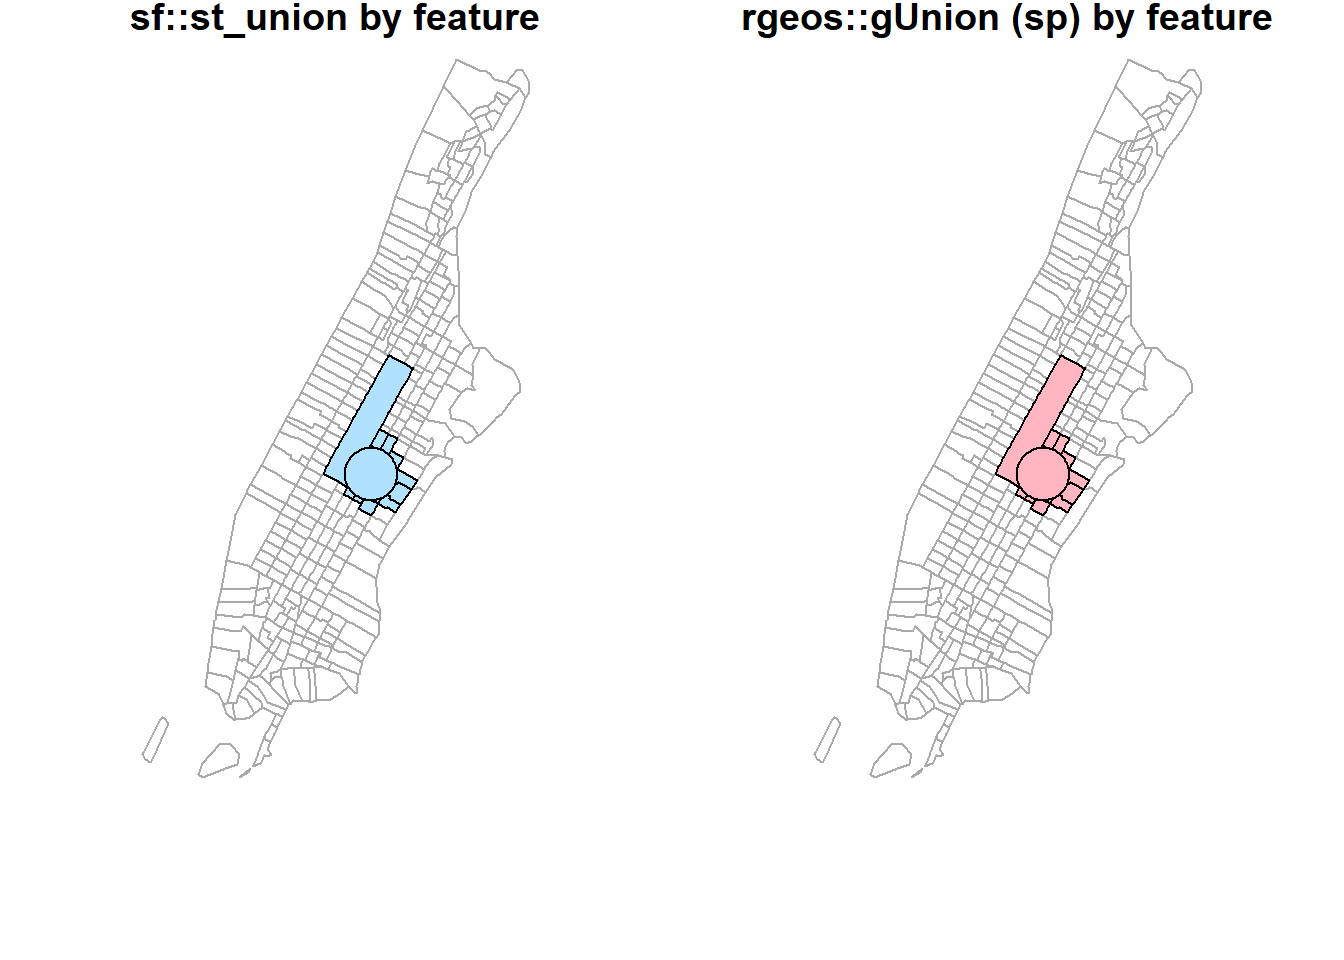
\includegraphics{R-spatial_files/figure-latex/geomOperationsBG-2.pdf}

\begin{Shaded}
\begin{Highlighting}[]
\FunctionTok{plot}\NormalTok{(}\FunctionTok{st\_geometry}\NormalTok{(man\_tracts\_sf), }\AttributeTok{border=}\StringTok{"\#aaaaaa"}\NormalTok{, }\AttributeTok{main=}\StringTok{\textquotesingle{}sf::st\_untion\textquotesingle{}}\NormalTok{)}
\FunctionTok{st\_union}\NormalTok{(buf\_sel\_sf, buf\_sf,}\AttributeTok{by\_feature =} \ConstantTok{FALSE}\NormalTok{) }\SpecialCharTok{\%\textgreater{}\%} 
  \FunctionTok{st\_geometry}\NormalTok{() }\SpecialCharTok{\%\textgreater{}\%} 
  \FunctionTok{plot}\NormalTok{(}\AttributeTok{col=}\StringTok{\textquotesingle{}lightskyblue1\textquotesingle{}}\NormalTok{, }\AttributeTok{add =}\NormalTok{ T)}

\FunctionTok{plot}\NormalTok{(}\FunctionTok{st\_geometry}\NormalTok{(man\_tracts\_sf), }\AttributeTok{border=}\StringTok{"\#aaaaaa"}\NormalTok{, }\AttributeTok{main=}\StringTok{\textquotesingle{}rgeos::gUnion (sp)\textquotesingle{}}\NormalTok{)}
\NormalTok{rgeos}\SpecialCharTok{::}\FunctionTok{gUnion}\NormalTok{(buf\_sf }\SpecialCharTok{\%\textgreater{}\%}\NormalTok{ sf}\SpecialCharTok{::}\FunctionTok{as\_Spatial}\NormalTok{(), }
\NormalTok{              buf\_sel\_sf }\SpecialCharTok{\%\textgreater{}\%}\NormalTok{ sf}\SpecialCharTok{::}\FunctionTok{as\_Spatial}\NormalTok{()) }\SpecialCharTok{\%\textgreater{}\%} 
  \FunctionTok{plot}\NormalTok{(}\AttributeTok{col=}\StringTok{\textquotesingle{}lightpink\textquotesingle{}}\NormalTok{, }\AttributeTok{add =}\NormalTok{ T)}
\end{Highlighting}
\end{Shaded}

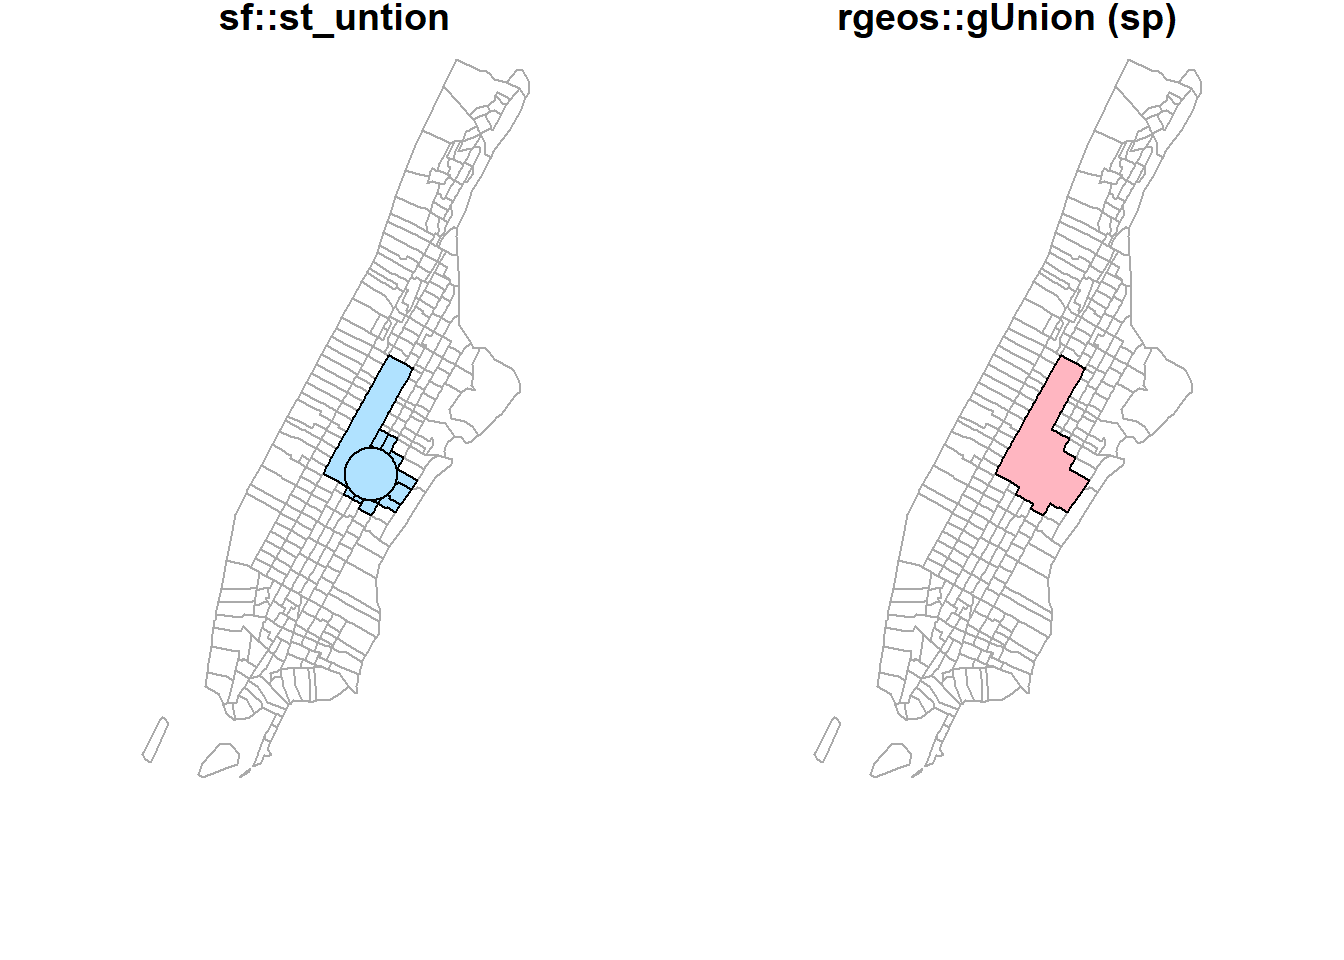
\includegraphics{R-spatial_files/figure-latex/geomOperationsBG-3.pdf}

\begin{Shaded}
\begin{Highlighting}[]
\FunctionTok{plot}\NormalTok{(}\FunctionTok{st\_geometry}\NormalTok{(man\_tracts\_sf), }\AttributeTok{border=}\StringTok{"\#aaaaaa"}\NormalTok{, }\AttributeTok{main=}\StringTok{\textquotesingle{}sf::st\_intersection\textquotesingle{}}\NormalTok{)}
\FunctionTok{st\_intersection}\NormalTok{(buf\_sel\_sf, buf\_sf) }\SpecialCharTok{\%\textgreater{}\%} 
  \FunctionTok{st\_geometry}\NormalTok{() }\SpecialCharTok{\%\textgreater{}\%} 
  \FunctionTok{plot}\NormalTok{(}\AttributeTok{col=}\StringTok{\textquotesingle{}lightskyblue1\textquotesingle{}}\NormalTok{, }\AttributeTok{add =}\NormalTok{ T)}

\FunctionTok{plot}\NormalTok{(}\FunctionTok{st\_geometry}\NormalTok{(man\_tracts\_sf), }\AttributeTok{border=}\StringTok{"\#aaaaaa"}\NormalTok{, }\AttributeTok{main=}\StringTok{\textquotesingle{}sf::st\_difference\textquotesingle{}}\NormalTok{)}
\FunctionTok{st\_difference}\NormalTok{(buf\_sel\_sf, buf\_sf) }\SpecialCharTok{\%\textgreater{}\%} \FunctionTok{st\_geometry}\NormalTok{() }\SpecialCharTok{\%\textgreater{}\%} 
  \FunctionTok{plot}\NormalTok{(}\AttributeTok{col=}\StringTok{\textquotesingle{}lightskyblue1\textquotesingle{}}\NormalTok{, }\AttributeTok{add =}\NormalTok{ T)}
\end{Highlighting}
\end{Shaded}

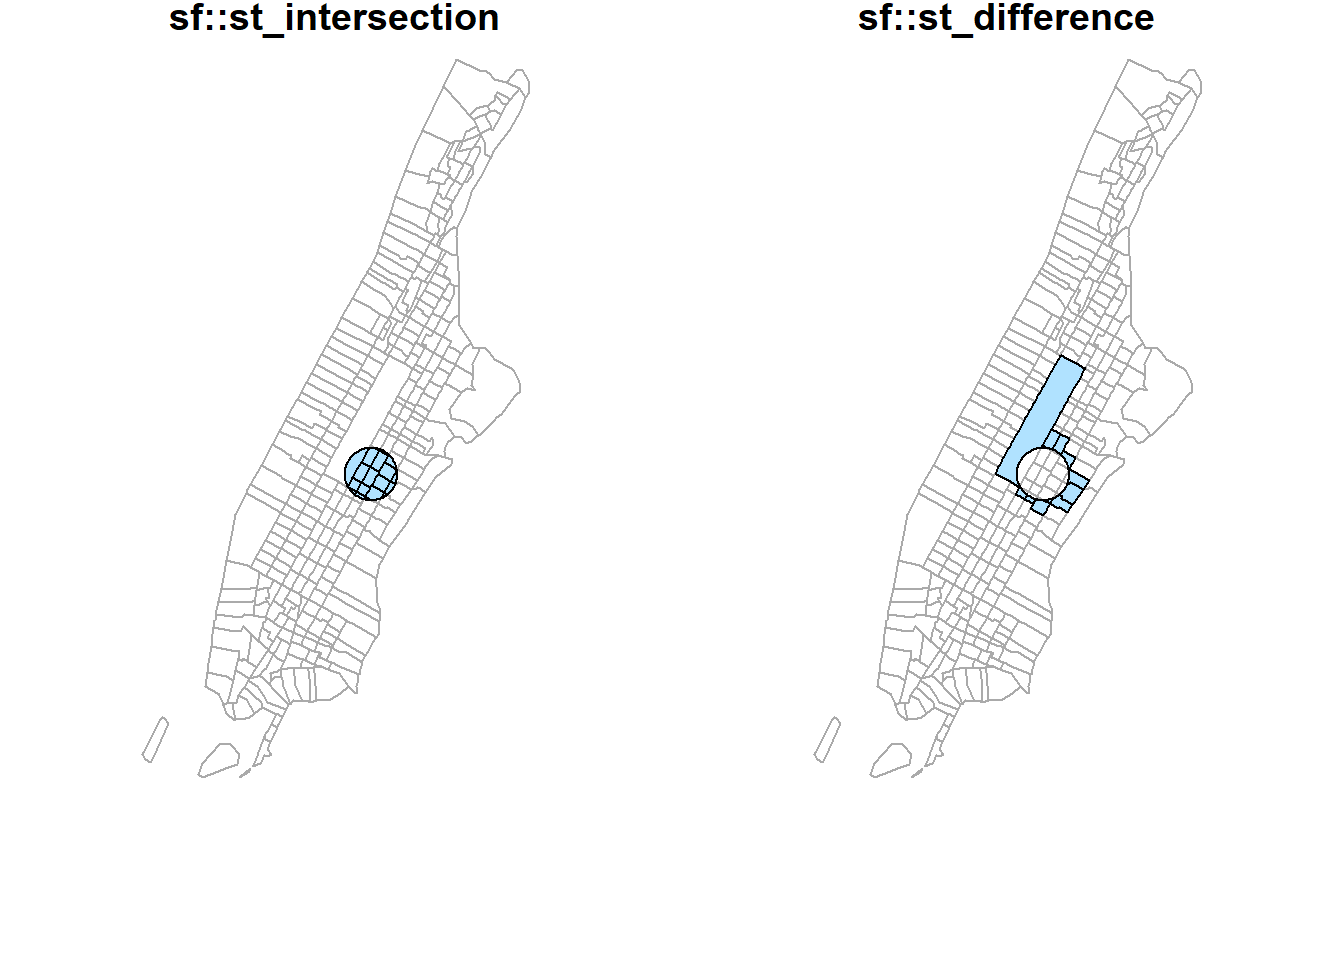
\includegraphics{R-spatial_files/figure-latex/geomOperationsBG-4.pdf}

\begin{Shaded}
\begin{Highlighting}[]
\FunctionTok{plot}\NormalTok{(}\FunctionTok{st\_geometry}\NormalTok{(man\_tracts\_sf), }\AttributeTok{border=}\StringTok{"\#aaaaaa"}\NormalTok{, }\AttributeTok{main=}\StringTok{\textquotesingle{}sf::st\_sym\_difference\textquotesingle{}}\NormalTok{)}
\FunctionTok{st\_sym\_difference}\NormalTok{(buf\_sel\_sf, buf\_sf) }\SpecialCharTok{\%\textgreater{}\%} 
  \FunctionTok{st\_geometry}\NormalTok{() }\SpecialCharTok{\%\textgreater{}\%} 
  \FunctionTok{plot}\NormalTok{(}\AttributeTok{col=}\StringTok{\textquotesingle{}lightskyblue1\textquotesingle{}}\NormalTok{, }\AttributeTok{add =}\NormalTok{ T)}

\FunctionTok{plot}\NormalTok{(}\FunctionTok{st\_geometry}\NormalTok{(man\_tracts\_sf), }\AttributeTok{border=}\StringTok{"\#aaaaaa"}\NormalTok{, }\AttributeTok{main=}\StringTok{\textquotesingle{}rgeos::gSysdifference (sp)\textquotesingle{}}\NormalTok{)}
\NormalTok{rgeos}\SpecialCharTok{::}\FunctionTok{gSymdifference}\NormalTok{(buf\_sf }\SpecialCharTok{\%\textgreater{}\%}\NormalTok{ sf}\SpecialCharTok{::}\FunctionTok{as\_Spatial}\NormalTok{(), }
\NormalTok{                      buf\_sel\_sf }\SpecialCharTok{\%\textgreater{}\%}\NormalTok{ sf}\SpecialCharTok{::}\FunctionTok{as\_Spatial}\NormalTok{(), }
                      \AttributeTok{drop\_lower\_td =} \ConstantTok{TRUE}\NormalTok{) }\SpecialCharTok{\%\textgreater{}\%} 
  \FunctionTok{plot}\NormalTok{(}\AttributeTok{col=}\StringTok{\textquotesingle{}lightpink\textquotesingle{}}\NormalTok{, }\AttributeTok{add =}\NormalTok{ T)}
\end{Highlighting}
\end{Shaded}

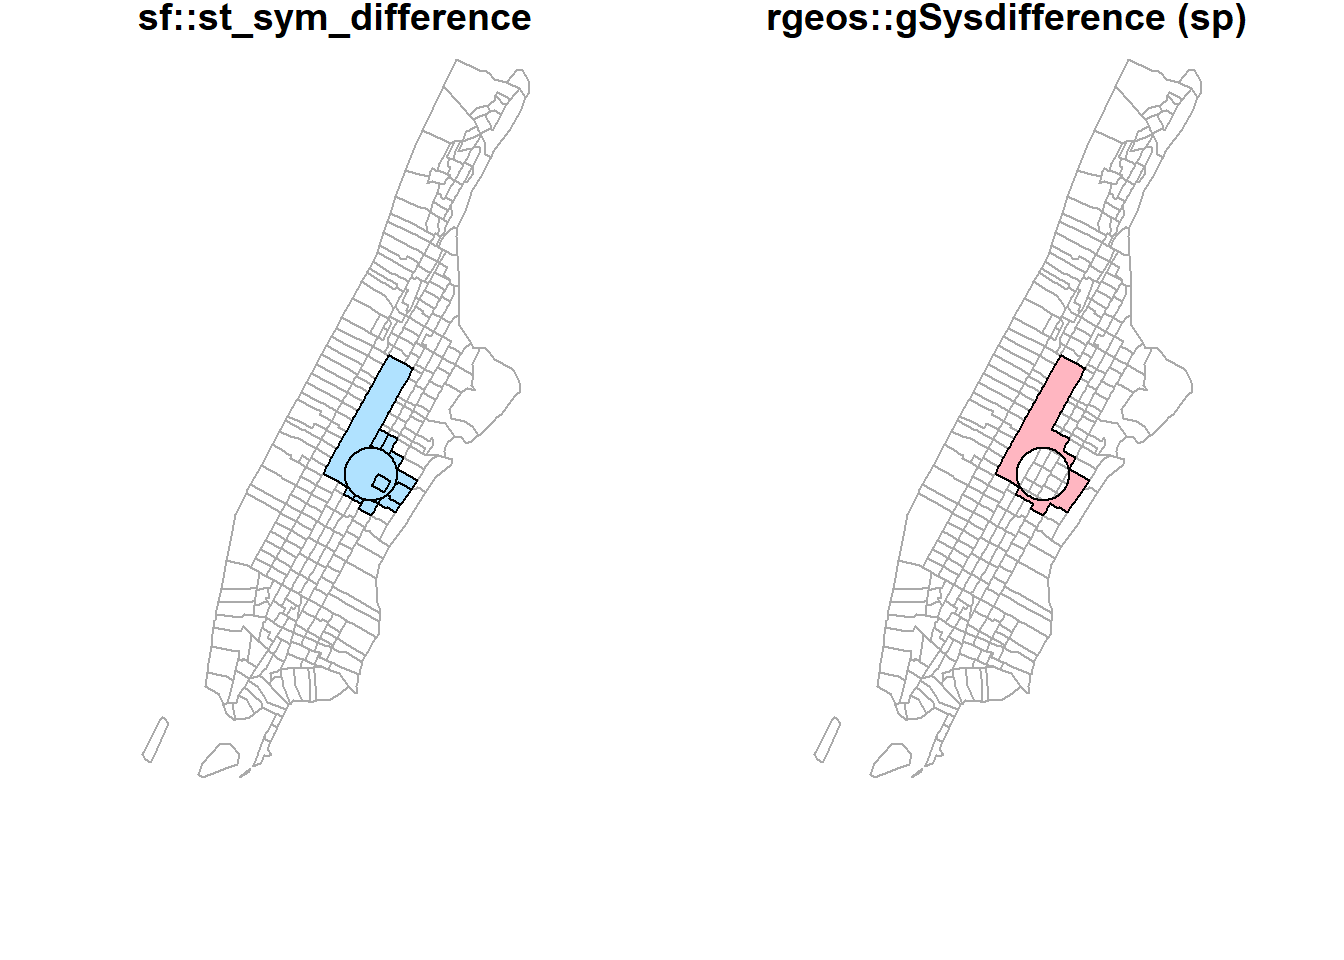
\includegraphics{R-spatial_files/figure-latex/geomOperationsBG-5.pdf}

\begin{Shaded}
\begin{Highlighting}[]
\FunctionTok{par}\NormalTok{(}\AttributeTok{mfrow=}\FunctionTok{c}\NormalTok{(}\DecValTok{1}\NormalTok{,}\DecValTok{2}\NormalTok{), }\AttributeTok{mar =} \FunctionTok{c}\NormalTok{(}\DecValTok{4}\NormalTok{, }\FloatTok{0.1}\NormalTok{, }\FloatTok{0.8}\NormalTok{, }\FloatTok{0.1}\NormalTok{))}

\FunctionTok{plot}\NormalTok{(}\FunctionTok{st\_geometry}\NormalTok{(man\_tracts\_sf), }\AttributeTok{border=}\StringTok{"\#aaaaaa"}\NormalTok{, }\AttributeTok{main=}\StringTok{\textquotesingle{}raster::union\textquotesingle{}}\NormalTok{)}
\NormalTok{raster}\SpecialCharTok{::}\FunctionTok{union}\NormalTok{(buf\_sf }\SpecialCharTok{\%\textgreater{}\%}\NormalTok{ sf}\SpecialCharTok{::}\FunctionTok{st\_geometry}\NormalTok{() }\SpecialCharTok{\%\textgreater{}\%}\NormalTok{ sf}\SpecialCharTok{::}\FunctionTok{as\_Spatial}\NormalTok{(),}
\NormalTok{              buf\_sel\_sf }\SpecialCharTok{\%\textgreater{}\%}\NormalTok{ sf}\SpecialCharTok{::}\FunctionTok{st\_geometry}\NormalTok{() }\SpecialCharTok{\%\textgreater{}\%}\NormalTok{ sf}\SpecialCharTok{::}\FunctionTok{as\_Spatial}\NormalTok{()) }\SpecialCharTok{\%\textgreater{}\%} 
  \FunctionTok{plot}\NormalTok{(}\AttributeTok{col=}\StringTok{\textquotesingle{}lightpink\textquotesingle{}}\NormalTok{, }\AttributeTok{add =}\NormalTok{ T)}
              
\FunctionTok{plot}\NormalTok{(}\FunctionTok{st\_geometry}\NormalTok{(man\_tracts\_sf), }\AttributeTok{border=}\StringTok{"\#aaaaaa"}\NormalTok{, }\AttributeTok{main=}\StringTok{\textquotesingle{}raster::instersect\textquotesingle{}}\NormalTok{)}
\NormalTok{raster}\SpecialCharTok{::}\FunctionTok{intersect}\NormalTok{(buf\_sf }\SpecialCharTok{\%\textgreater{}\%}\NormalTok{ sf}\SpecialCharTok{::}\FunctionTok{st\_geometry}\NormalTok{() }\SpecialCharTok{\%\textgreater{}\%}\NormalTok{ sf}\SpecialCharTok{::}\FunctionTok{as\_Spatial}\NormalTok{(), }
\NormalTok{                  buf\_sel\_sf }\SpecialCharTok{\%\textgreater{}\%}\NormalTok{ sf}\SpecialCharTok{::}\FunctionTok{st\_geometry}\NormalTok{() }\SpecialCharTok{\%\textgreater{}\%}\NormalTok{ sf}\SpecialCharTok{::}\FunctionTok{as\_Spatial}\NormalTok{()) }\SpecialCharTok{\%\textgreater{}\%} 
  \FunctionTok{plot}\NormalTok{(}\AttributeTok{col=}\StringTok{\textquotesingle{}lightpink\textquotesingle{}}\NormalTok{, }\AttributeTok{add =}\NormalTok{ T)}
\end{Highlighting}
\end{Shaded}

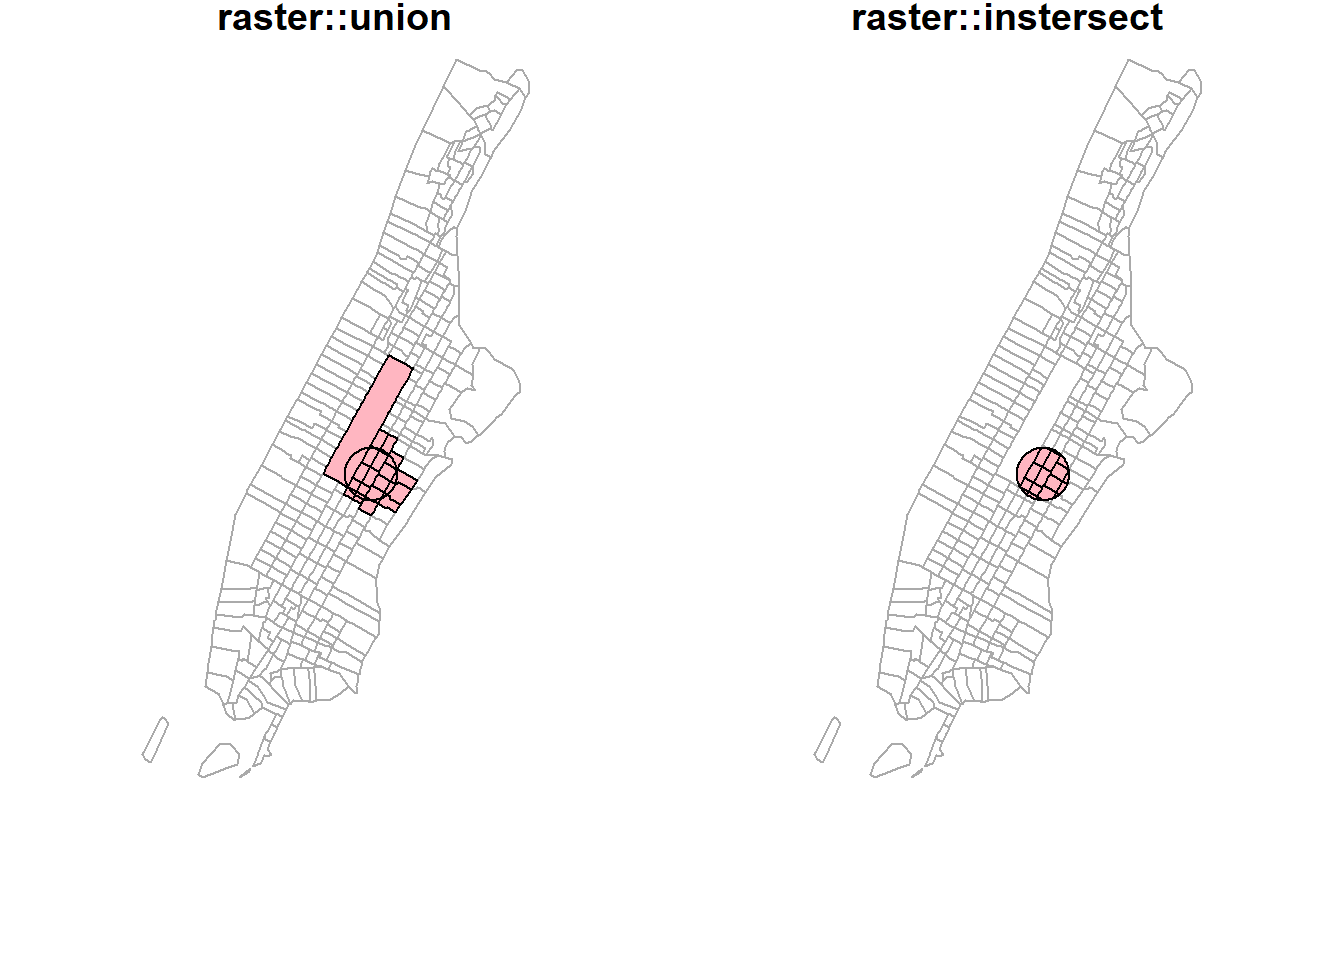
\includegraphics{R-spatial_files/figure-latex/geomOperationsBG-6.pdf}

Earlier, we used \textbf{\emph{group\_by}} + \textbf{\emph{summarize}} \textbf{\emph{(sf)}} and \textbf{\emph{aggregate}} \textbf{\emph{(sp)}} to conduct spatial aggregation or spatial join. When these functions apply to a single spatial object (unary operations), they could do the dissolve. Note that those internal ``sliver'' polygons are caused by inaccurate boundaries. For example, two neighboring polygons should have exactly the same boundary at where they touch. But if not, those sliver polygons will be produced during spatial operations. That also partially explains why sf performs very bad because sf assumes data strictly following Simple Features specifications. Obviously, the Philly data do not.

\begin{Shaded}
\begin{Highlighting}[]
\FunctionTok{par}\NormalTok{(}\AttributeTok{mfrow=}\FunctionTok{c}\NormalTok{(}\DecValTok{1}\NormalTok{,}\DecValTok{2}\NormalTok{), }\AttributeTok{mar =} \FunctionTok{c}\NormalTok{(}\DecValTok{4}\NormalTok{, }\FloatTok{0.1}\NormalTok{, }\FloatTok{0.8}\NormalTok{, }\FloatTok{0.1}\NormalTok{));}
\CommentTok{\#philly\_sf\_merged \%\textgreater{}\% st\_geometry() \%\textgreater{}\% plot();}
\NormalTok{nyc\_sf\_merged }\SpecialCharTok{\%\textgreater{}\%} 
\NormalTok{  dplyr}\SpecialCharTok{::}\FunctionTok{mutate}\NormalTok{(}\AttributeTok{incomeFactor =} \FunctionTok{cut}\NormalTok{(MEDHHINC, }
                                   \FunctionTok{c}\NormalTok{(}\DecValTok{0}\NormalTok{, }\DecValTok{30000}\NormalTok{, }\DecValTok{80000}\NormalTok{, }\ConstantTok{Inf}\NormalTok{), }
                                   \FunctionTok{c}\NormalTok{(}\StringTok{\textquotesingle{}Low\textquotesingle{}}\NormalTok{, }\StringTok{\textquotesingle{}Medium\textquotesingle{}}\NormalTok{, }\StringTok{\textquotesingle{}High\textquotesingle{}}\NormalTok{))) }\SpecialCharTok{\%\textgreater{}\%}
\NormalTok{  dplyr}\SpecialCharTok{::}\FunctionTok{select}\NormalTok{(incomeFactor, geometry ) }\SpecialCharTok{\%\textgreater{}\%}
  \FunctionTok{group\_by}\NormalTok{(incomeFactor) }\SpecialCharTok{\%\textgreater{}\%}
  \FunctionTok{summarise}\NormalTok{() }\SpecialCharTok{\%\textgreater{}\%} \FunctionTok{plot}\NormalTok{(}\AttributeTok{main=}\StringTok{"group\_by+summarize"}\NormalTok{);}
\end{Highlighting}
\end{Shaded}

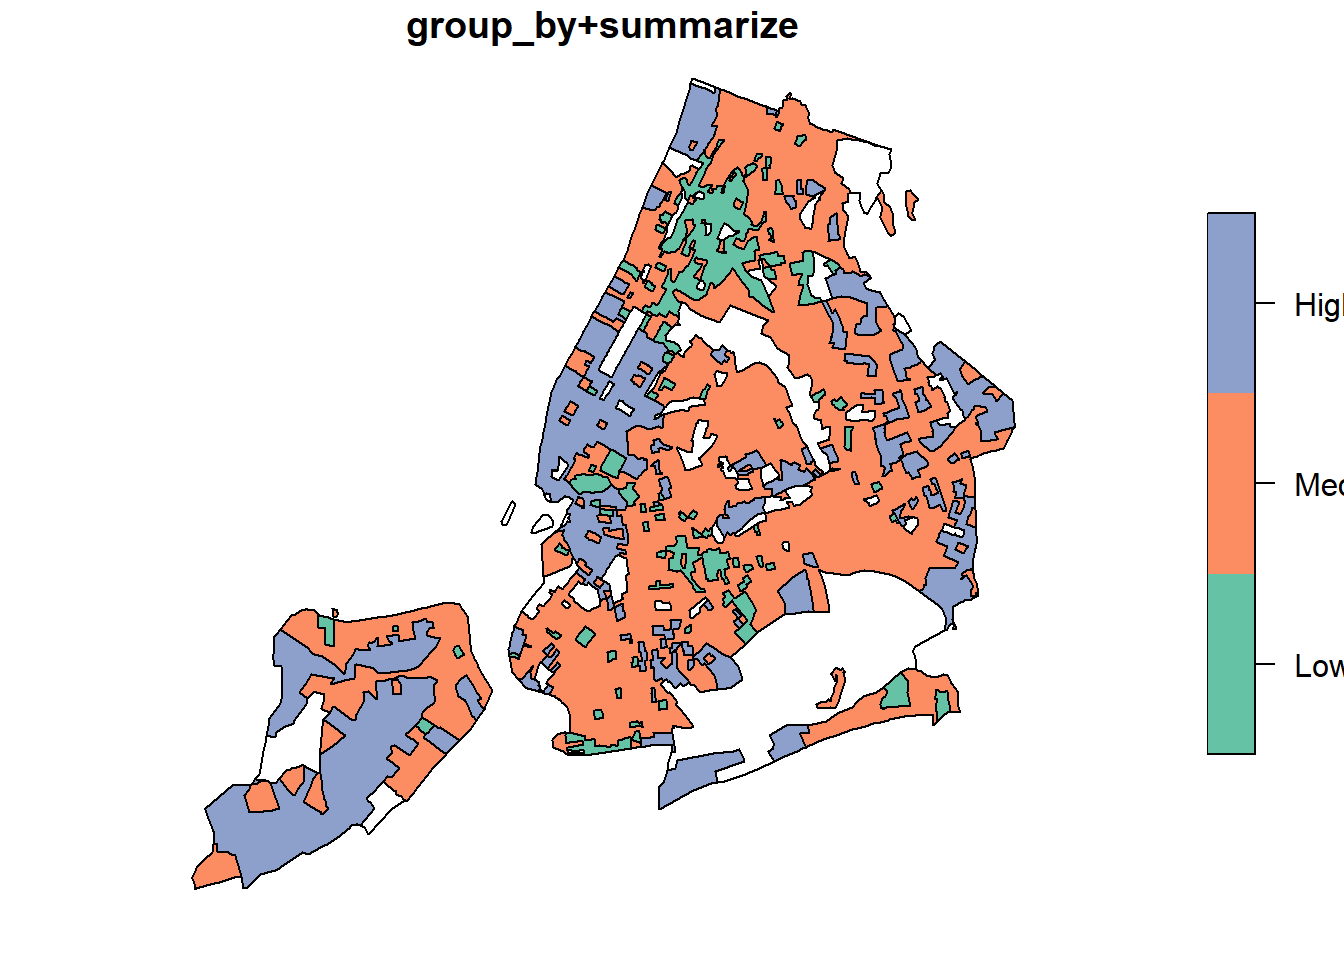
\includegraphics[width=0.9\linewidth]{R-spatial_files/figure-latex/dissolveSF-1}

\begin{Shaded}
\begin{Highlighting}[]
\NormalTok{groupFactor }\OtherTok{\textless{}{-}}  \FunctionTok{cut}\NormalTok{(nyc\_sf\_merged}\SpecialCharTok{$}\NormalTok{MEDHHINC,}
                    \FunctionTok{c}\NormalTok{(}\DecValTok{0}\NormalTok{, }\DecValTok{30000}\NormalTok{, }\DecValTok{80000}\NormalTok{, }\ConstantTok{Inf}\NormalTok{), }
                    \FunctionTok{c}\NormalTok{(}\StringTok{\textquotesingle{}Low\textquotesingle{}}\NormalTok{, }\StringTok{\textquotesingle{}Medium\textquotesingle{}}\NormalTok{, }\StringTok{\textquotesingle{}High\textquotesingle{}}\NormalTok{));}

\NormalTok{nyc\_sf\_merged }\SpecialCharTok{\%\textgreater{}\%}
\NormalTok{  dplyr}\SpecialCharTok{::}\FunctionTok{select}\NormalTok{(MEDHHINC, geometry ) }\SpecialCharTok{\%\textgreater{}\%}
  \FunctionTok{aggregate}\NormalTok{(}\AttributeTok{by =} \FunctionTok{list}\NormalTok{(}\AttributeTok{FemDocLevel =}\NormalTok{ groupFactor), sum) }\SpecialCharTok{\%\textgreater{}\%} 
\NormalTok{  magrittr}\SpecialCharTok{::}\FunctionTok{extract}\NormalTok{(}\StringTok{\textquotesingle{}FemDocLevel\textquotesingle{}}\NormalTok{) }\SpecialCharTok{\%\textgreater{}\%} \FunctionTok{plot}\NormalTok{(}\AttributeTok{main=}\StringTok{"dissolve by aggregate"}\NormalTok{)}
\end{Highlighting}
\end{Shaded}

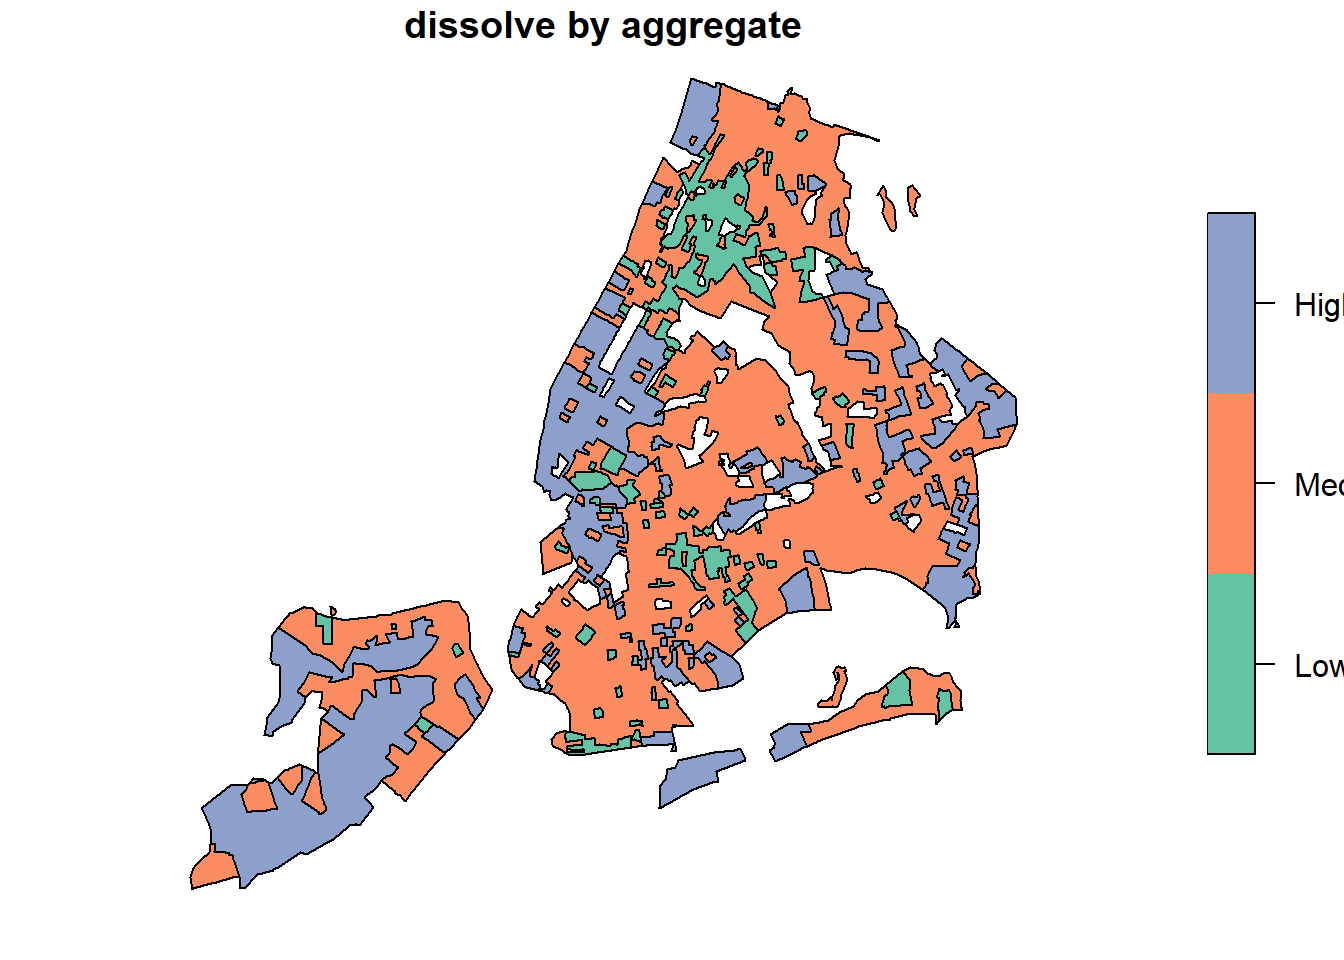
\includegraphics[width=0.9\linewidth]{R-spatial_files/figure-latex/dissolveSF-2}

\hypertarget{information-for-raster-operations}{%
\section{Information for Raster Operations}\label{information-for-raster-operations}}

Some helpful packages that deal with raster data:

\begin{itemize}
\tightlist
\item
  \href{https://CRAN.R-project.org/package=landscapetools}{\texttt{landscapetools}} provides utility functions to complete tasks involved in common landscape analysis.
\item
  \href{https://CRAN.R-project.org/package=getlandsat}{\texttt{getlandsat}}: Get Landsat 8 Data from \href{https://registry.opendata.aws/landsat-8/}{Amazon Public Data Sets}
\item
  \href{https://CRAN.R-project.org/package=MODIStsp}{\texttt{MODIStsp}}: automates the creation of time series of rasters derived from MODIS Land Products data
\item
  \href{https://cran.r-project.org/package=FedData}{\texttt{FedData}}: Download geospatial Data from federated data sources, including the The National Elevation Dataset digital elevation models, the Global Historical Climatology Network, the National Land Cover Database, and more.
\end{itemize}

\hypertarget{lab-assignment-1}{%
\section{Lab Assignment}\label{lab-assignment-1}}

The second lab is to aggregate data from different sources to the zip codes as the core covid-19 data are available at that scale.

Main tasks for the second lab are:

\begin{enumerate}
\def\labelenumi{\arabic{enumi}.}
\tightlist
\item
  Join the COVID-19 data to the NYC zip code area data (sf or sp polygons).
\item
  Aggregate the NYC food retails store data (points) to the zip code data, so that we know how many retail stores in each zip code area. Note that not all locations are for food retail. And we need to choose the specific types according to the data.
\item
  Aggregate the NYC health facilities (points) to the zip code data. Similarly, choose appropriate subtypes such as nursing homes from the facilities.
\item
  Join the Census ACS population, race, and age data to the NYC Planning Census Tract Data.
\item
  Aggregate the ACS census data to zip code area data.
\end{enumerate}

In the end, we should have the confirmed and tested cases of covid-19, numbers of specific types of food stores, numbers of specific types of health facilities, and population (total population, elderly, by race, etc.) at the zip code level. We should also have boroughs, names, etc. for each zip code area.

\hypertarget{mapping}{%
\chapter{Making Maps in R}\label{mapping}}

\begin{quote}
Learning Objectives

\begin{itemize}
\tightlist
\item
  plot an \textbf{\emph{sf}} object
\item
  create a choropleth map with \textbf{\emph{ggplot}}

  \begin{itemize}
  \tightlist
  \item
    add a basemap with \textbf{\emph{ggmap}}
  \item
    use \textbf{\emph{RColorBrewer}} to improve legend colors
  \item
    use \textbf{\emph{classInt}} to improve legend breaks
  \end{itemize}
\item
  create a choropleth map with \textbf{\emph{tmap}}
\item
  create an interactive map with \textbf{\emph{leaflet}}
\end{itemize}
\end{quote}

\begin{center}\rule{0.5\linewidth}{0.5pt}\end{center}

In the preceding examples we have used the base \texttt{plot} command to take a quick look at our spatial objects. In this section we will explore several alternatives to map spatial data with R. For more packages see the ``Visualization'' section of the \href{https://cran.r-project.org/web/views/Spatial.html}{CRAN Task View}.

Mapping packages are in the process of keeping up with the development of the new \emph{sf} package, so they typically accept both \emph{sp} and \emph{sf} objects. However, there are a few exceptions.

Of the packages shown here \texttt{spplot()}, which is part of the good old \emph{sp} package, only takes \emph{sp} objects. The \href{https://github.com/tidyverse/ggplot2/releases}{development version of \emph{ggplot2}} can take \emph{sf} objects, though \texttt{ggmap} \href{https://github.com/tidyverse/ggplot2/issues/2130}{seems to still have issues} with \emph{sf}. Both \emph{tmap} and \emph{leaflet} can also handle both \emph{sp} and \emph{sf} objects.

\hypertarget{plotting-simple-features-sf-with-plot}{%
\section{\texorpdfstring{Plotting simple features (\emph{sf}) with \texttt{plot}}{Plotting simple features (sf) with plot}}\label{plotting-simple-features-sf-with-plot}}

As we have already briefly seen, the \emph{sf} package extends the base \texttt{plot} command, so it can be used on \emph{sf} objects. If used without any arguments it will plot all the attributes using up to 10 ``pretty'' breaks. See its document ion by typing \texttt{?sf::plot.sf} on the console.

\begin{Shaded}
\begin{Highlighting}[]
\CommentTok{\# Read Manhattan noise complaints data aggregtated in census tracts}
\NormalTok{man\_noise\_rate\_sf }\OtherTok{\textless{}{-}}  \FunctionTok{st\_read}\NormalTok{(}\StringTok{"./data/nyc/man\_noise\_rate.shp"}\NormalTok{, }\AttributeTok{quiet =} \ConstantTok{TRUE}\NormalTok{)}
\CommentTok{\# Read homicides points and transform it to the same CRS as census tract above}
\NormalTok{man\_noises\_pt }\OtherTok{\textless{}{-}}\NormalTok{ sf}\SpecialCharTok{::}\FunctionTok{st\_read}\NormalTok{(}\StringTok{\textquotesingle{}./data/nyc/ManhattanNoise.shp\textquotesingle{}}\NormalTok{) }\SpecialCharTok{\%\textgreater{}\%}
\NormalTok{  sf}\SpecialCharTok{::}\FunctionTok{st\_transform}\NormalTok{(sf}\SpecialCharTok{::}\FunctionTok{st\_crs}\NormalTok{(man\_noise\_rate\_sf));}
\end{Highlighting}
\end{Shaded}

\begin{verbatim}
#> Reading layer `ManhattanNoise' from data source 
#>   `D:\Cloud_Drive\Dropbox (Hunter College)\Workspace\RSpace\R-Spatial_Book\data\nyc\ManhattanNoise.shp' 
#>   using driver `ESRI Shapefile'
#> Simple feature collection with 68582 features and 5 fields
#> Geometry type: POINT
#> Dimension:     XY
#> Bounding box:  xmin: -74.018 ymin: 40.69889 xmax: -73.90809 ymax: 40.87783
#> Geodetic CRS:  WGS 84
\end{verbatim}

\begin{Shaded}
\begin{Highlighting}[]
\CommentTok{\# Simple plot.sf}
\FunctionTok{plot}\NormalTok{(man\_noise\_rate\_sf)}
\end{Highlighting}
\end{Shaded}

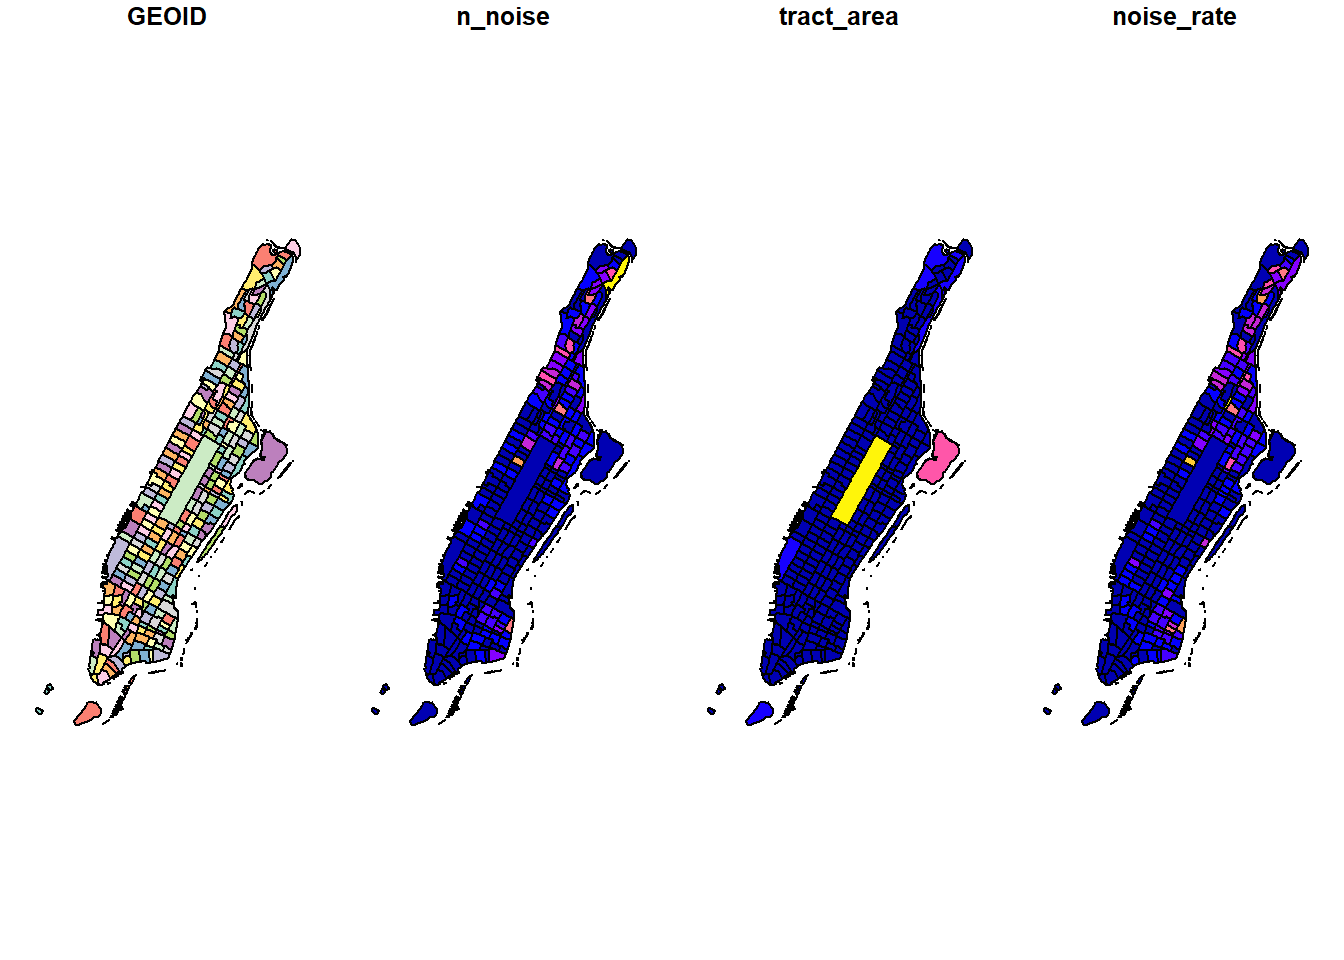
\includegraphics{R-spatial_files/figure-latex/sf-plot-default-1.pdf}

To plot a single attribute we need to provide an object of class \emph{sf}, like so:

\begin{Shaded}
\begin{Highlighting}[]
\CommentTok{\# Plot a single column (attribute)}
\FunctionTok{plot}\NormalTok{(man\_noise\_rate\_sf}\SpecialCharTok{$}\NormalTok{noise\_rate) }\CommentTok{\# this is a numeric vector!}
\end{Highlighting}
\end{Shaded}

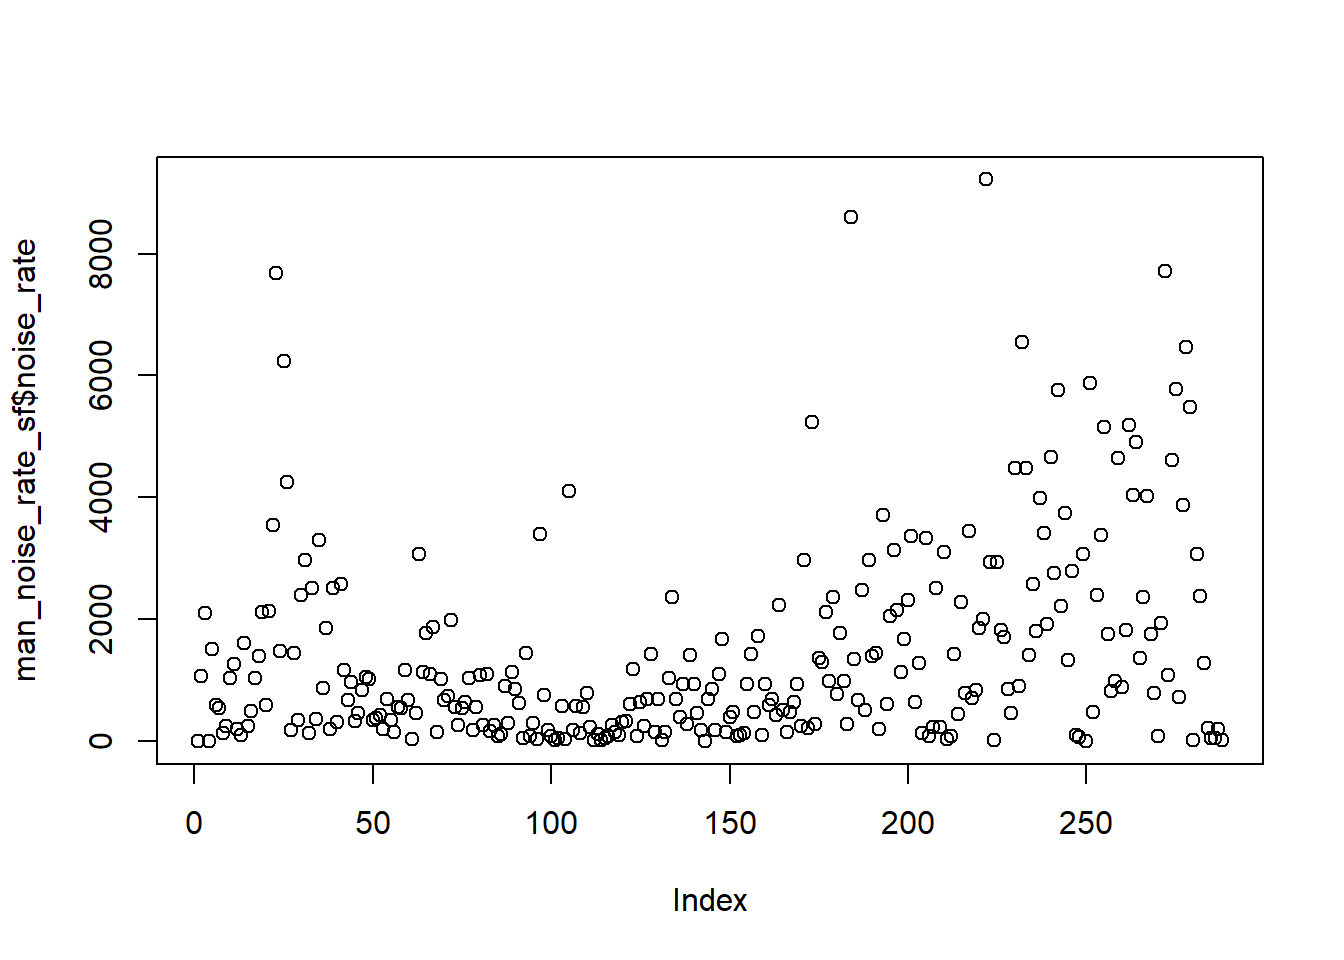
\includegraphics{R-spatial_files/figure-latex/sf-plot-single-1.pdf}

\begin{Shaded}
\begin{Highlighting}[]
\FunctionTok{plot}\NormalTok{(man\_noise\_rate\_sf[}\StringTok{"noise\_rate"}\NormalTok{]) }\CommentTok{\# this plot one column}
\end{Highlighting}
\end{Shaded}

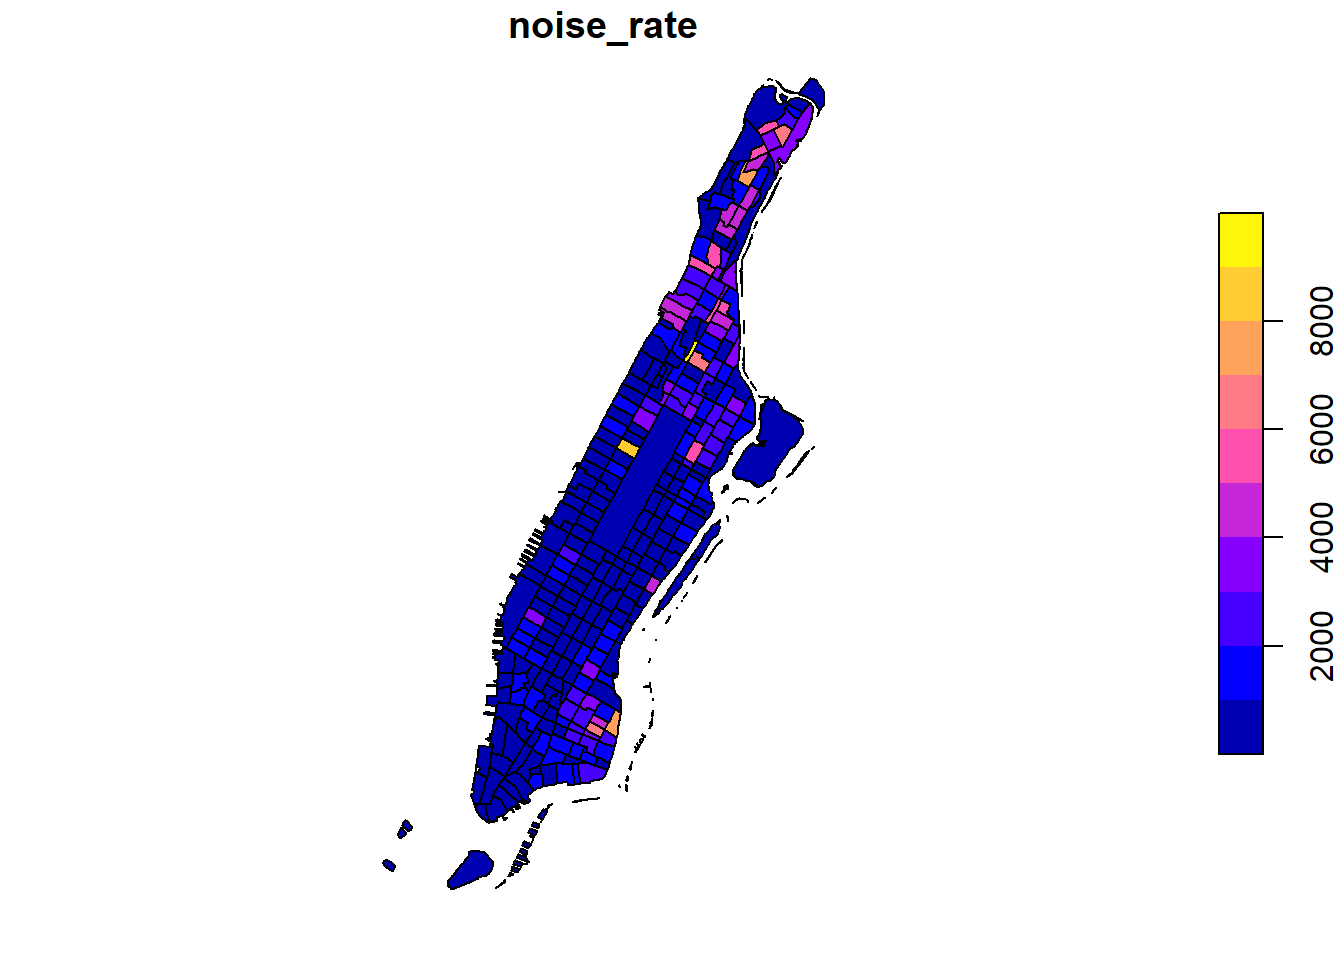
\includegraphics{R-spatial_files/figure-latex/sf-plot-single-2.pdf}

Since our values are unevenly distributed\ldots:

\includegraphics{R-spatial_files/figure-latex/unnamed-chunk-8-1.pdf}

\ldots we might want to set the breaks to quantiles in order to better distinguish the census tracts with low values. This can be done by using the \texttt{breaks} argument for the sf plot function.

\begin{Shaded}
\begin{Highlighting}[]
\FunctionTok{plot}\NormalTok{(man\_noise\_rate\_sf[}\StringTok{"noise\_rate"}\NormalTok{], }
     \AttributeTok{main =} \StringTok{"Manhattan Noise Complaint (per square km)"}\NormalTok{, }
     \AttributeTok{breaks =} \StringTok{"quantile"}\NormalTok{,}
     \AttributeTok{border =} \ConstantTok{NA}\NormalTok{,}
     \AttributeTok{graticule =} \ConstantTok{TRUE}\NormalTok{)}
\end{Highlighting}
\end{Shaded}

\includegraphics{R-spatial_files/figure-latex/sf-plot-qantile-1.pdf}

Using the \texttt{reset=FALSE} parameter in the first \texttt{plot} on \texttt{*sf*} object and \texttt{add=TRUE} on following plots, we can plot multiple layers on the map.

\begin{Shaded}
\begin{Highlighting}[]
\NormalTok{ptColor }\OtherTok{\textless{}{-}} \FunctionTok{rgb}\NormalTok{(}\FloatTok{0.1}\NormalTok{,}\FloatTok{0.9}\NormalTok{,}\FloatTok{0.1}\NormalTok{,}\FloatTok{0.4}\NormalTok{);}
\FunctionTok{plot}\NormalTok{(man\_noise\_rate\_sf[}\StringTok{"noise\_rate"}\NormalTok{], }
     \AttributeTok{main =} \StringTok{"Manhattan Noise Complaint (per square km)"}\NormalTok{, }
     \AttributeTok{breaks =} \StringTok{"quantile"}\NormalTok{,}
     \AttributeTok{border =} \ConstantTok{NA}\NormalTok{,}
     \AttributeTok{graticule =} \FunctionTok{st\_crs}\NormalTok{(}\DecValTok{4326}\NormalTok{),}
     \AttributeTok{axes=}\ConstantTok{TRUE}\NormalTok{,}
     \AttributeTok{reset=}\ConstantTok{FALSE}\NormalTok{)}
\FunctionTok{plot}\NormalTok{(man\_noises\_pt[}\StringTok{"incdnt\_z"}\NormalTok{], }\AttributeTok{pch=}\DecValTok{19}\NormalTok{, }\AttributeTok{col=}\NormalTok{ptColor, }\AttributeTok{cex=}\FloatTok{0.1}\NormalTok{, }\AttributeTok{add=}\ConstantTok{TRUE}\NormalTok{)}
\end{Highlighting}
\end{Shaded}

\includegraphics{R-spatial_files/figure-latex/addPlotSf-1.pdf}

We can change the color palette using a library called \texttt{RColorBrewer}\footnote{This is not the only way to provide color palettes. You can create your customized palette in many different ways or simply as a vector of hexbin color codes, like \texttt{c(\ "\#FDBB84"\ "\#FC8D59"\ "\#EF6548")}.}. For more about ColorBrewer palettes read \href{http://colorbrewer2.org}{this}.

To make the color palettes from ColorBrewer available as R palettes we use the \texttt{brewer.pal()} function. It takes two arguments:
- the number of different colors desired and
- the name of the palette as character string.

We select 7 colors from the `Orange-Red' palette and assign it to an object \texttt{pal}.

\begin{Shaded}
\begin{Highlighting}[]
\FunctionTok{library}\NormalTok{(RColorBrewer)}
\NormalTok{pal }\OtherTok{\textless{}{-}} \FunctionTok{brewer.pal}\NormalTok{(}\DecValTok{7}\NormalTok{, }\StringTok{"OrRd"}\NormalTok{) }\CommentTok{\# we select 7 colors from the palette}
\FunctionTok{class}\NormalTok{(pal)}
\end{Highlighting}
\end{Shaded}

\begin{verbatim}
#> [1] "character"
\end{verbatim}

Finally, we add this to the plot

\begin{Shaded}
\begin{Highlighting}[]
\FunctionTok{plot}\NormalTok{(man\_noise\_rate\_sf[}\StringTok{"noise\_rate"}\NormalTok{], }
     \AttributeTok{main =} \StringTok{"Manhattan Noise Complaint per square km"}\NormalTok{, }
     \AttributeTok{breaks =} \StringTok{"quantile"}\NormalTok{, }\AttributeTok{nbreaks =} \DecValTok{7}\NormalTok{,}
     \AttributeTok{pal =}\NormalTok{ pal,}
     \AttributeTok{graticule =} \FunctionTok{st\_crs}\NormalTok{(}\DecValTok{4326}\NormalTok{),}
     \AttributeTok{axes=}\ConstantTok{TRUE}\NormalTok{,}
     \AttributeTok{reset=}\ConstantTok{FALSE}\NormalTok{)}
\FunctionTok{plot}\NormalTok{(man\_noises\_pt[}\StringTok{"incdnt\_z"}\NormalTok{], }\AttributeTok{pch=}\DecValTok{19}\NormalTok{, }\AttributeTok{col=}\NormalTok{ptColor, }\AttributeTok{cex=}\FloatTok{0.1}\NormalTok{, }\AttributeTok{add=}\ConstantTok{TRUE}\NormalTok{)}
\end{Highlighting}
\end{Shaded}

\includegraphics{R-spatial_files/figure-latex/sf-plot-legend-1.pdf}

We can also choose to plot multiple columns side by side using \texttt{plot.sf}. But this is only good for simple illustration as it is harder to customize the two plots.

\begin{Shaded}
\begin{Highlighting}[]
\FunctionTok{plot}\NormalTok{(man\_noise\_rate\_sf[}\FunctionTok{c}\NormalTok{(}\StringTok{"n\_noise"}\NormalTok{,}\StringTok{"noise\_rate"}\NormalTok{)], }\AttributeTok{breaks =} \StringTok{\textquotesingle{}jenks\textquotesingle{}}\NormalTok{) }\CommentTok{\# this plot multiple columns}
\end{Highlighting}
\end{Shaded}

\includegraphics{R-spatial_files/figure-latex/sf-plot-multiple-1.pdf}

\hypertarget{choropleth-mapping-with-spplot}{%
\section{\texorpdfstring{Choropleth mapping with \texttt{spplot}}{Choropleth mapping with spplot}}\label{choropleth-mapping-with-spplot}}

\emph{sp} comes with a plot command \texttt{spplot()}, which takes \texttt{Spatial*} objects to plot. \texttt{spplot()} is one of the earlier functions around to plot geographic objects.

Like plot, by default \texttt{spplot} maps everything it can find in the attribute table. Sometimes this does not work, depending on the data types in the attribute table. In order to select specific values to map we can provide the \texttt{spplot} function with the name (or names) of the attribute variable(s) we want to plot. It is the name of the column of the \texttt{Spatial*Dataframe} as character string (or a vector if several).

\begin{Shaded}
\begin{Highlighting}[]
\FunctionTok{spplot}\NormalTok{(man\_noise\_rate\_sf }\SpecialCharTok{\%\textgreater{}\%}\NormalTok{ sf}\SpecialCharTok{::}\FunctionTok{as\_Spatial}\NormalTok{(), }\StringTok{"noise\_rate"}\NormalTok{)}
\end{Highlighting}
\end{Shaded}

\includegraphics{R-spatial_files/figure-latex/spplot-single-1.pdf}

Many improvements can be made here as well, below is an example\footnote{For more details see Chaps 2 and 3 in \href{https://asdar-book.org}{Applied Spatial Data Analysis with R}. Also, \texttt{spplot} is a wrapper for the \href{https://cran.r-project.org/package=lattice}{\texttt{lattice} package}, see there for more advanced options.} \footnote{For the correction of breaks after using classIntervals with spplot/levelplot see here \url{http://r.789695.n4.nabble.com/SpatialPolygon-with-the-max-value-gets-no-color-assigned-in-spplot-function-when-using-quot-at-quot-r-td4654672.html}}.

\begin{Shaded}
\begin{Highlighting}[]
\CommentTok{\# quantile breaks}
\FunctionTok{require}\NormalTok{(classInt)}
\NormalTok{breaks\_qt }\OtherTok{\textless{}{-}} \FunctionTok{classIntervals}\NormalTok{(man\_noise\_rate\_sf}\SpecialCharTok{$}\NormalTok{noise\_rate, }\AttributeTok{n =} \DecValTok{7}\NormalTok{, }\AttributeTok{style =} \StringTok{"quantile"}\NormalTok{)}
\NormalTok{br }\OtherTok{\textless{}{-}}\NormalTok{ breaks\_qt}\SpecialCharTok{$}\NormalTok{brks }\SpecialCharTok{\%\textgreater{}\%} \FunctionTok{as.integer}\NormalTok{()}
\NormalTok{offs }\OtherTok{\textless{}{-}} \FloatTok{0.0000001} 
\NormalTok{br[}\DecValTok{1}\NormalTok{] }\OtherTok{\textless{}{-}}\NormalTok{ br[}\DecValTok{1}\NormalTok{] }\SpecialCharTok{{-}}\NormalTok{ offs }
\NormalTok{br[}\FunctionTok{length}\NormalTok{(br)] }\OtherTok{\textless{}{-}}\NormalTok{ br[}\FunctionTok{length}\NormalTok{(br)] }\SpecialCharTok{+}\NormalTok{ offs }
\CommentTok{\# categoreis for choropleth map}
\NormalTok{man\_noise\_rate\_sf}\SpecialCharTok{$}\NormalTok{noise\_rate\_bracket }\OtherTok{\textless{}{-}} \FunctionTok{cut}\NormalTok{(man\_noise\_rate\_sf}\SpecialCharTok{$}\NormalTok{noise\_rate, br)}
\CommentTok{\# plot}
\FunctionTok{spplot}\NormalTok{(man\_noise\_rate\_sf }\SpecialCharTok{\%\textgreater{}\%}\NormalTok{ sf}\SpecialCharTok{::}\FunctionTok{as\_Spatial}\NormalTok{(), }\StringTok{"noise\_rate\_bracket"}\NormalTok{, }\AttributeTok{col.regions=}\NormalTok{pal, }\AttributeTok{main =} \StringTok{"Manhattan Noise Complaint Density (per square km)"}\NormalTok{)}
\end{Highlighting}
\end{Shaded}

\includegraphics{R-spatial_files/figure-latex/spplot-final-map-1.pdf}

\hypertarget{choropleth-mapping-with-ggplot2}{%
\section{\texorpdfstring{Choropleth mapping with \emph{ggplot2}}{Choropleth mapping with ggplot2}}\label{choropleth-mapping-with-ggplot2}}

\href{http://ggplot2.org/}{\emph{ggplot2}} is a widely used and powerful plotting library for R. It is not specifically geared towards mapping, but one can generate great maps.

As we have learned from previous sections, the \texttt{ggplot()} syntax is different from the previous as a plot is built up by adding components with a \texttt{+}. You can start with a layer showing the raw data then add layers of annotations and statistical summaries. This allows to easily superimpose either different visualizations of one dataset (e.g.~a scatterplot and a fitted line) or different datasets (like different layers of the same geographical area)\footnote{See Wilkinson L (2005): ``The grammar of graphics''. Statistics and computing, 2nd ed.~Springer, New York.}.

For an introduction to \texttt{ggplot} check out \href{http://link.springer.com/book/10.1007\%2F978-3-319-24277-4}{this book by the package creator} or \href{http://ggplot2.tidyverse.org/}{this} for more pointers.

In order to build a plot you start with initializing a ggplot object. In order to do that
\texttt{ggplot()} takes:

\begin{itemize}
\tightlist
\item
  a data argument usually a \textbf{dataframe} and
\item
  a mapping argument where x and y values to be plotted are supplied.
\end{itemize}

In addition, minimally a geometry to be used to determine how the values should be displayed. This is to be added after an \texttt{+}.

\begin{verbatim}
ggplot(data = my_data_frame, mapping = aes(x = name_of_column_with_x_value, y = name_of_column_with_y_value)) +
  geom_point()
\end{verbatim}

Or shorter:

\begin{verbatim}
ggplot(my_data_frame, aes(name_of_column_with_x_value, name_of_column_with_y_value)) +
  geom_point()
\end{verbatim}

\hypertarget{basic-sf-plotting-using-ggplot}{%
\subsection{\texorpdfstring{Basic \emph{sf} plotting using \texttt{ggplot}}{Basic sf plotting using ggplot}}\label{basic-sf-plotting-using-ggplot}}

The great news is that \textbf{\texttt{ggplot} can plot \emph{sf} objects directly} by using \texttt{geom\_sf}. So all we have to do is:

\begin{Shaded}
\begin{Highlighting}[]
\FunctionTok{ggplot}\NormalTok{(man\_noise\_rate\_sf) }\SpecialCharTok{+} 
  \FunctionTok{geom\_sf}\NormalTok{(}\FunctionTok{aes}\NormalTok{(}\AttributeTok{fill=}\NormalTok{noise\_rate))}
\end{Highlighting}
\end{Shaded}

\includegraphics{R-spatial_files/figure-latex/ggplot-sf-1.pdf}

Homicide rate is a continuous variable and is plotted by \texttt{ggplot} as such. If we wanted to plot our map as a `true' choropleth map we need to convert our continuous variable into a categorical one, according to whichever brackets we want to use.

This requires two steps:

\begin{itemize}
\tightlist
\item
  Determine the breaks with a ``style'', i.e.~the method or algorithm used to categorize data.
\item
  Add a categorical variable to the object which assigns each continuous value to a bracket.
\end{itemize}

We will use the \texttt{classInt} package to explicitly determine the breaks.

\begin{Shaded}
\begin{Highlighting}[]
\FunctionTok{require}\NormalTok{(classInt)}

\CommentTok{\# get quantile breaks. Add .00001 offset to catch the lowest value}
\NormalTok{breaks\_qt }\OtherTok{\textless{}{-}} \FunctionTok{classIntervals}\NormalTok{(}\FunctionTok{c}\NormalTok{(}\FunctionTok{min}\NormalTok{(man\_noise\_rate\_sf}\SpecialCharTok{$}\NormalTok{noise\_rate) }\SpecialCharTok{{-}}\NormalTok{ .}\DecValTok{00001}\NormalTok{,}
\NormalTok{                              man\_noise\_rate\_sf}\SpecialCharTok{$}\NormalTok{noise\_rate), }\AttributeTok{n =} \DecValTok{7}\NormalTok{, }\AttributeTok{style =} \StringTok{"quantile"}\NormalTok{)}

\NormalTok{breaks\_qt}
\end{Highlighting}
\end{Shaded}

\begin{verbatim}
#> style: quantile
#> [0.3316134,93.8384)  [93.8384,288.3639)  [288.3639,553.946)  [553.946,877.4583) 
#>                  42                  41                  41                  41 
#> [877.4583,1452.304) [1452.304,2567.292) [2567.292,9217.026] 
#>                  41                  41                  42
\end{verbatim}

OK. We can retrieve the breaks with \texttt{breaks\$brks}.

We use \texttt{cut} to divide \texttt{noise\_rate} into intervals and code them according to which interval they are in.

Lastly, we can use \texttt{scale\_fill\_brewer} and add our color palette.

\begin{Shaded}
\begin{Highlighting}[]
\NormalTok{man\_noise\_rate\_sf }\OtherTok{\textless{}{-}} \FunctionTok{mutate}\NormalTok{(man\_noise\_rate\_sf, }\AttributeTok{noise\_rate\_cat =} \FunctionTok{cut}\NormalTok{(noise\_rate, breaks\_qt}\SpecialCharTok{$}\NormalTok{brks)) }

\FunctionTok{ggplot}\NormalTok{(man\_noise\_rate\_sf) }\SpecialCharTok{+} 
  \FunctionTok{geom\_sf}\NormalTok{(}\FunctionTok{aes}\NormalTok{(}\AttributeTok{fill=}\NormalTok{noise\_rate\_cat)) }\SpecialCharTok{+}
  \FunctionTok{scale\_fill\_brewer}\NormalTok{(}\AttributeTok{palette =} \StringTok{"OrRd"}\NormalTok{, }\AttributeTok{name=}\StringTok{\textquotesingle{}Per SQKM\textquotesingle{}}\NormalTok{) }\SpecialCharTok{+}
  \FunctionTok{coord\_sf}\NormalTok{(}\AttributeTok{xlim =} \FunctionTok{c}\NormalTok{(}\SpecialCharTok{{-}}\FloatTok{74.06}\NormalTok{, }\SpecialCharTok{{-}}\FloatTok{73.85}\NormalTok{), }\AttributeTok{default\_crs =}\NormalTok{ sf}\SpecialCharTok{::}\FunctionTok{st\_crs}\NormalTok{(}\DecValTok{4326}\NormalTok{) ) }\SpecialCharTok{+}
  \FunctionTok{labs}\NormalTok{(}\AttributeTok{x=}\StringTok{\textquotesingle{}Longitude\textquotesingle{}}\NormalTok{, }\AttributeTok{y=}\StringTok{\textquotesingle{}Latitude\textquotesingle{}}\NormalTok{, }
       \AttributeTok{title=}\StringTok{\textquotesingle{}Manhattan Noise Complaint Rate\textquotesingle{}}\NormalTok{,}
       \AttributeTok{caption =} \StringTok{\textquotesingle{}Data Source: []\textquotesingle{}}\NormalTok{);}
\end{Highlighting}
\end{Shaded}

\includegraphics{R-spatial_files/figure-latex/ggplot-sf-categorical-1.pdf}

\hypertarget{multi-layer-plotting}{%
\subsection{Multi-layer plotting}\label{multi-layer-plotting}}

Similarly, we can add multiple layers to the \texttt{ggplot}.

\begin{Shaded}
\begin{Highlighting}[]
\FunctionTok{ggplot}\NormalTok{(man\_noise\_rate\_sf) }\SpecialCharTok{+} 
  \FunctionTok{geom\_sf}\NormalTok{(}\FunctionTok{aes}\NormalTok{(}\AttributeTok{fill=}\NormalTok{noise\_rate\_cat)) }\SpecialCharTok{+}
  \FunctionTok{geom\_sf}\NormalTok{(}\AttributeTok{data=}\NormalTok{man\_noises\_pt, }\AttributeTok{colour=}\NormalTok{ptColor, }\AttributeTok{size=}\FloatTok{0.1}\NormalTok{) }\SpecialCharTok{+}
  \FunctionTok{scale\_fill\_brewer}\NormalTok{(}\AttributeTok{palette =} \StringTok{"OrRd"}\NormalTok{, }\AttributeTok{name=}\StringTok{\textquotesingle{}Noise Complaint Per SQKM\textquotesingle{}}\NormalTok{) }\SpecialCharTok{+}
  \FunctionTok{coord\_sf}\NormalTok{(}\AttributeTok{xlim =} \FunctionTok{c}\NormalTok{(}\SpecialCharTok{{-}}\FloatTok{74.06}\NormalTok{, }\SpecialCharTok{{-}}\FloatTok{73.85}\NormalTok{), }\AttributeTok{default\_crs =}\NormalTok{ sf}\SpecialCharTok{::}\FunctionTok{st\_crs}\NormalTok{(}\DecValTok{4326}\NormalTok{) ) }\SpecialCharTok{+}
  \FunctionTok{labs}\NormalTok{(}\AttributeTok{x=}\StringTok{\textquotesingle{}Longitude\textquotesingle{}}\NormalTok{, }\AttributeTok{y=}\StringTok{\textquotesingle{}Latitude\textquotesingle{}}\NormalTok{, }
       \AttributeTok{title=}\StringTok{\textquotesingle{}Manhattan Noise Complaint Rate\textquotesingle{}}\NormalTok{,}
       \AttributeTok{caption =} \StringTok{\textquotesingle{}Data Source: [...]\textquotesingle{}}\NormalTok{);}
\end{Highlighting}
\end{Shaded}

\includegraphics{R-spatial_files/figure-latex/ggplot-sf-multi-layer-1.pdf}

\hypertarget{label-spatial-objects}{%
\subsection{Label spatial objects}\label{label-spatial-objects}}

With \texttt{geom\_sf\_text} and \texttt{geom\_sf\_label} functions, we can add labels to mapped spatial objects. \texttt{geom\_sf\_label} draws a rectangle behind the text, therefore making good contrast. As in other GIS software, labeling is complicated because there would be many conflicts among labels. The results of automatic labeling is rarely satisfactory and up to the standard of cartography or academic publication. Even though packages like \texttt{ggrepel} greatly help avoid overlapping labels, manual adjustments are often necessary and preferred.

\begin{Shaded}
\begin{Highlighting}[]
\FunctionTok{ggplot}\NormalTok{(man\_noise\_rate\_sf) }\SpecialCharTok{+} 
  \FunctionTok{geom\_sf}\NormalTok{(}\FunctionTok{aes}\NormalTok{(}\AttributeTok{fill=}\NormalTok{noise\_rate\_cat)) }\SpecialCharTok{+}
  \FunctionTok{geom\_sf}\NormalTok{(}\AttributeTok{data=}\NormalTok{man\_noises\_pt, }\AttributeTok{colour=}\NormalTok{ptColor, }\AttributeTok{size=}\FloatTok{0.1}\NormalTok{) }\SpecialCharTok{+}
  \FunctionTok{geom\_sf\_label}\NormalTok{(}\AttributeTok{data =}\NormalTok{ man\_noise\_rate\_sf }\SpecialCharTok{\%\textgreater{}\%}\NormalTok{ dplyr}\SpecialCharTok{::}\FunctionTok{filter}\NormalTok{(n\_noise }\SpecialCharTok{\textgreater{}} \DecValTok{1000}\NormalTok{),}
                \FunctionTok{aes}\NormalTok{(}\AttributeTok{label =}\NormalTok{ n\_noise),}
                \AttributeTok{label.size =}\NormalTok{ .}\DecValTok{09}\NormalTok{,}
                \AttributeTok{size =} \DecValTok{3}\NormalTok{) }\SpecialCharTok{+}
  \FunctionTok{scale\_fill\_brewer}\NormalTok{(}\AttributeTok{palette =} \StringTok{"OrRd"}\NormalTok{, }\AttributeTok{name=}\StringTok{\textquotesingle{}Homicide Per SQKM\textquotesingle{}}\NormalTok{) }\SpecialCharTok{+}
  \FunctionTok{coord\_sf}\NormalTok{(}\AttributeTok{xlim =} \FunctionTok{c}\NormalTok{(}\SpecialCharTok{{-}}\FloatTok{74.06}\NormalTok{, }\SpecialCharTok{{-}}\FloatTok{73.85}\NormalTok{), }\AttributeTok{default\_crs =}\NormalTok{ sf}\SpecialCharTok{::}\FunctionTok{st\_crs}\NormalTok{(}\DecValTok{4326}\NormalTok{) ) }\SpecialCharTok{+}
  \FunctionTok{labs}\NormalTok{(}\AttributeTok{x=}\StringTok{\textquotesingle{}Longitude\textquotesingle{}}\NormalTok{, }\AttributeTok{y=}\StringTok{\textquotesingle{}Latitude\textquotesingle{}}\NormalTok{, }
       \AttributeTok{title=}\StringTok{\textquotesingle{}Manhattan Noise Complaint Rate\textquotesingle{}}\NormalTok{,}
       \AttributeTok{caption =} \StringTok{\textquotesingle{}Data Source: [...]\textquotesingle{}}\NormalTok{);}
\end{Highlighting}
\end{Shaded}

\begin{verbatim}
#> Warning in st_point_on_surface.sfc(sf::st_zm(x)): st_point_on_surface may not
#> give correct results for longitude/latitude data
\end{verbatim}

\includegraphics{R-spatial_files/figure-latex/ggplot-sf-label-1.pdf}

Using \texttt{ggrepel} helps disperse those labels.

\begin{Shaded}
\begin{Highlighting}[]
\FunctionTok{require}\NormalTok{(ggrepel);}
\NormalTok{labelCoords }\OtherTok{\textless{}{-}}\NormalTok{ man\_noise\_rate\_sf }\SpecialCharTok{\%\textgreater{}\%}\NormalTok{ sf}\SpecialCharTok{::}\FunctionTok{st\_centroid}\NormalTok{() }\SpecialCharTok{\%\textgreater{}\%}
\NormalTok{  dplyr}\SpecialCharTok{::}\FunctionTok{filter}\NormalTok{(n\_noise }\SpecialCharTok{\textgreater{}} \DecValTok{1000}\NormalTok{) }\SpecialCharTok{\%\textgreater{}\%}
\NormalTok{  sf}\SpecialCharTok{::}\FunctionTok{st\_coordinates}\NormalTok{();}

\NormalTok{labelData }\OtherTok{\textless{}{-}}\NormalTok{ man\_noise\_rate\_sf }\SpecialCharTok{\%\textgreater{}\%}\NormalTok{ sf}\SpecialCharTok{::}\FunctionTok{st\_centroid}\NormalTok{() }\SpecialCharTok{\%\textgreater{}\%}
\NormalTok{  dplyr}\SpecialCharTok{::}\FunctionTok{filter}\NormalTok{(n\_noise }\SpecialCharTok{\textgreater{}} \DecValTok{1000}\NormalTok{) }\SpecialCharTok{\%\textgreater{}\%}
\NormalTok{  dplyr}\SpecialCharTok{::}\FunctionTok{mutate}\NormalTok{(}\AttributeTok{x =}\NormalTok{ labelCoords[,}\DecValTok{1}\NormalTok{], }\AttributeTok{y=}\NormalTok{labelCoords[,}\DecValTok{2}\NormalTok{])}
                     

\FunctionTok{ggplot}\NormalTok{(man\_noise\_rate\_sf) }\SpecialCharTok{+} 
  \FunctionTok{geom\_sf}\NormalTok{(}\FunctionTok{aes}\NormalTok{(}\AttributeTok{fill=}\NormalTok{noise\_rate\_cat)) }\SpecialCharTok{+}
  \CommentTok{\#geom\_sf(data=man\_noises\_pt, colour=ptColor, size=0.1) +}
  \FunctionTok{geom\_label\_repel}\NormalTok{(}\AttributeTok{data =}\NormalTok{ labelData,}
                   \FunctionTok{aes}\NormalTok{(}\AttributeTok{x=}\NormalTok{x,}\AttributeTok{y=}\NormalTok{y,}\AttributeTok{label =}\NormalTok{ n\_noise),}
                   \AttributeTok{label.size =}\NormalTok{ .}\DecValTok{09}\NormalTok{,}
                   \AttributeTok{size =} \DecValTok{3}\NormalTok{,}
                   \AttributeTok{segment.color =} \FunctionTok{rgb}\NormalTok{(}\FloatTok{0.5}\NormalTok{,}\FloatTok{0.5}\NormalTok{,}\FloatTok{0.9}\NormalTok{),}
                   \AttributeTok{segment.size =} \FloatTok{0.8}\NormalTok{) }\SpecialCharTok{+}
  \FunctionTok{scale\_fill\_brewer}\NormalTok{(}\AttributeTok{palette =} \StringTok{"OrRd"}\NormalTok{, }\AttributeTok{name=}\StringTok{\textquotesingle{}Homicide Per SQKM\textquotesingle{}}\NormalTok{) }\SpecialCharTok{+}
  \FunctionTok{coord\_sf}\NormalTok{(}\AttributeTok{xlim =} \FunctionTok{c}\NormalTok{(}\SpecialCharTok{{-}}\FloatTok{74.06}\NormalTok{, }\SpecialCharTok{{-}}\FloatTok{73.85}\NormalTok{), }\AttributeTok{default\_crs =}\NormalTok{ sf}\SpecialCharTok{::}\FunctionTok{st\_crs}\NormalTok{(}\DecValTok{4326}\NormalTok{) ) }\SpecialCharTok{+}
  \FunctionTok{labs}\NormalTok{(}\AttributeTok{x=}\StringTok{\textquotesingle{}Longitude\textquotesingle{}}\NormalTok{, }\AttributeTok{y=}\StringTok{\textquotesingle{}Latitude\textquotesingle{}}\NormalTok{, }
       \AttributeTok{title=}\StringTok{\textquotesingle{}Manhattan Noise Complaint Rate\textquotesingle{}}\NormalTok{,}
       \AttributeTok{caption =} \StringTok{\textquotesingle{}Data Source: [...]\textquotesingle{}}\NormalTok{);}
\end{Highlighting}
\end{Shaded}

\includegraphics{R-spatial_files/figure-latex/ggplot-sf-repel-label-1.pdf}

\hypertarget{adding-basemaps-with-ggmap}{%
\subsection{\texorpdfstring{Adding basemaps with \texttt{ggmap}}{Adding basemaps with ggmap}}\label{adding-basemaps-with-ggmap}}

\texttt{ggmap} builds on \texttt{ggplot} and allows to pull in tiled basemaps from different services, like Google Maps, OpenStreetMaps, or Stamen Maps\footnote{Google now \href{https://cloud.google.com/maps-platform/.}{requires an API key}. Cloudmade maps retired its API so it is no longer possible to be used as basemap. \href{https://CRAN.R-project.org/package=RgoogleMaps}{\texttt{RgoogleMaps}} is another library that provides an interface to query the Google server for static maps.}.

So let's overlay the map from above on a terrain map we pull from Stamen.

If you have a valid Google Maps API key, the following method still works. First we use the \texttt{get\_map()} command from \texttt{ggmap} to pull down the basemap. We need to tell it the location or the boundaries of the map, the zoom level, and what kind of map service we like (default is Google terrain). It will actually download the tile. \texttt{get\_map()} returns a ggmap object, name it \texttt{man\_basemap}. In order to view the map we then use \texttt{ggmap()}.

Currently, only the Stamen Maps allows R code to retrieve base maps without API keys. And we need to specifically call the function \texttt{get\_stamenmap} to acquire the basemap. If we plan to make multiples maps for the same area, it is better to save it to a variable and reuse it.

\begin{Shaded}
\begin{Highlighting}[]
\FunctionTok{require}\NormalTok{(ggmap)}

\CommentTok{\# We can get a simple basemap. Adjust zoom with the map extent. }
\CommentTok{\# Higher zoom means more details but needs more time to load.}
\CommentTok{\# Start from small and increase to an appropriate level. Will learn more on this.}

\CommentTok{\# In most cases we can use the extent of the data to retrieve the basemap}
\CommentTok{\# Note those services require boundary in geographic coordinates }
\CommentTok{\# and we also want to expand a little bit to completely contain the data ranges.}
\NormalTok{mapBound }\OtherTok{\textless{}{-}}\NormalTok{ man\_noise\_rate\_sf }\SpecialCharTok{\%\textgreater{}\%}\NormalTok{ sf}\SpecialCharTok{::}\FunctionTok{st\_transform}\NormalTok{(}\DecValTok{4326}\NormalTok{) }\SpecialCharTok{\%\textgreater{}\%} 
  \FunctionTok{st\_bbox}\NormalTok{() }\SpecialCharTok{\%\textgreater{}\%} \FunctionTok{st\_as\_sfc}\NormalTok{() }\SpecialCharTok{\%\textgreater{}\%} \FunctionTok{st\_buffer}\NormalTok{(}\FloatTok{0.02}\NormalTok{) }\SpecialCharTok{\%\textgreater{}\%}
  \FunctionTok{st\_bbox}\NormalTok{() }\SpecialCharTok{\%\textgreater{}\%} \FunctionTok{as.numeric}\NormalTok{()}

\CommentTok{\# but for the long shape of Manhattan, it might be better to manually choose the basemap}
\NormalTok{mapBound }\OtherTok{\textless{}{-}} \FunctionTok{c}\NormalTok{(}\SpecialCharTok{{-}}\FloatTok{74.06}\NormalTok{, }\FloatTok{40.682}\NormalTok{, }\SpecialCharTok{{-}}\FloatTok{73.85}\NormalTok{, }\FloatTok{40.883}\NormalTok{)}

\NormalTok{man\_basemap }\OtherTok{\textless{}{-}}\NormalTok{ ggmap}\SpecialCharTok{::}\FunctionTok{get\_stamenmap}\NormalTok{(}\AttributeTok{bbox =}\NormalTok{ mapBound, }\AttributeTok{zoom =} \DecValTok{11}\NormalTok{, }\AttributeTok{messaging =} \ConstantTok{FALSE}\NormalTok{, }\AttributeTok{maptype =} \StringTok{\textquotesingle{}terrain{-}background\textquotesingle{}}\NormalTok{)}

\FunctionTok{ggmap}\NormalTok{(man\_basemap)}
\end{Highlighting}
\end{Shaded}

\includegraphics{R-spatial_files/figure-latex/ggmap-getmap-1.pdf}

Then we can reuse the code from the ggplot example above, just replacing the first line, where we initialized a ggplot object above

\begin{verbatim}
    ggplot() + 
\end{verbatim}

with the line to call our basemap:

\begin{verbatim}
    ggmap(man_basemap) +
\end{verbatim}

We also have to set \texttt{inherit.aes} to \texttt{FALSE}, so it overrides the default aesthetics (from the ggmap object).

\begin{Shaded}
\begin{Highlighting}[]
\FunctionTok{ggmap}\NormalTok{(man\_basemap) }\SpecialCharTok{+}
  \FunctionTok{geom\_sf}\NormalTok{(}\AttributeTok{data =}\NormalTok{ man\_noise\_rate\_sf, }\FunctionTok{aes}\NormalTok{(}\AttributeTok{fill=}\NormalTok{noise\_rate\_cat), }\AttributeTok{inherit.aes =} \ConstantTok{FALSE}\NormalTok{) }\SpecialCharTok{+}
  \FunctionTok{scale\_fill\_brewer}\NormalTok{(}\AttributeTok{palette =} \StringTok{"OrRd"}\NormalTok{)}
\end{Highlighting}
\end{Shaded}

\includegraphics{R-spatial_files/figure-latex/ggmap-plot-misaligned-1.pdf}

Note that if the data are in a local map projection, We need to set our CRS to WGS84, which is the one the tiles are downloaded in. We can add \texttt{coord\_sf} to do this:

\begin{Shaded}
\begin{Highlighting}[]
\FunctionTok{ggmap}\NormalTok{(man\_basemap) }\SpecialCharTok{+}
    \FunctionTok{geom\_sf}\NormalTok{(}\AttributeTok{data =}\NormalTok{ man\_noise\_rate\_sf, }\FunctionTok{aes}\NormalTok{(}\AttributeTok{fill=}\NormalTok{noise\_rate\_cat), }\AttributeTok{inherit.aes =} \ConstantTok{FALSE}\NormalTok{) }\SpecialCharTok{+}
    \FunctionTok{scale\_fill\_brewer}\NormalTok{(}\AttributeTok{palette =} \StringTok{"OrRd"}\NormalTok{) }\SpecialCharTok{+}
    \FunctionTok{coord\_sf}\NormalTok{(}\AttributeTok{crs =} \FunctionTok{st\_crs}\NormalTok{(}\DecValTok{4326}\NormalTok{))}
\end{Highlighting}
\end{Shaded}

\includegraphics{R-spatial_files/figure-latex/ggmap-plot-aligned-1.pdf}

The \texttt{ggmap} package also includes functions for distance calculations, geocoding, and calculating routes.

\hypertarget{arrange-and-export-plots}{%
\subsection{Arrange and export plots}\label{arrange-and-export-plots}}

As we have learned before, we can plot these maps to an external file using \texttt{ggsave} or \texttt{ggexport}. With \texttt{ggarrange}, we can also make a nice layout of multiple maps. We can also create a better defined device first and the plot maps on that device.

\begin{Shaded}
\begin{Highlighting}[]
\NormalTok{g1 }\OtherTok{\textless{}{-}} \FunctionTok{ggmap}\NormalTok{(man\_basemap) }\SpecialCharTok{+}
    \FunctionTok{geom\_sf}\NormalTok{(}\AttributeTok{data =}\NormalTok{ man\_noise\_rate\_sf, }\FunctionTok{aes}\NormalTok{(}\AttributeTok{fill=}\NormalTok{noise\_rate\_cat), }\AttributeTok{inherit.aes =} \ConstantTok{FALSE}\NormalTok{) }\SpecialCharTok{+}
    \FunctionTok{scale\_fill\_brewer}\NormalTok{(}\AttributeTok{palette =} \StringTok{"OrRd"}\NormalTok{) }\SpecialCharTok{+}
    \FunctionTok{coord\_sf}\NormalTok{(}\AttributeTok{crs =} \FunctionTok{st\_crs}\NormalTok{(}\DecValTok{4326}\NormalTok{))}

\NormalTok{g2 }\OtherTok{\textless{}{-}} \FunctionTok{ggplot}\NormalTok{(man\_noise\_rate\_sf) }\SpecialCharTok{+} 
  \FunctionTok{geom\_sf}\NormalTok{(}\FunctionTok{aes}\NormalTok{(}\AttributeTok{fill=}\NormalTok{noise\_rate\_cat)) }\SpecialCharTok{+}
  \FunctionTok{geom\_sf}\NormalTok{(}\AttributeTok{data=}\NormalTok{man\_noises\_pt, }\AttributeTok{colour=}\NormalTok{ptColor, }\AttributeTok{size=}\FloatTok{0.1}\NormalTok{) }\SpecialCharTok{+}
  \FunctionTok{scale\_fill\_brewer}\NormalTok{(}\AttributeTok{palette =} \StringTok{"OrRd"}\NormalTok{, }\AttributeTok{name=}\StringTok{\textquotesingle{}Noise Complaint Per SQKM\textquotesingle{}}\NormalTok{) }\SpecialCharTok{+}
  \FunctionTok{coord\_sf}\NormalTok{(}\AttributeTok{xlim =} \FunctionTok{c}\NormalTok{(}\SpecialCharTok{{-}}\FloatTok{74.06}\NormalTok{, }\SpecialCharTok{{-}}\FloatTok{73.85}\NormalTok{), }\AttributeTok{default\_crs =}\NormalTok{ sf}\SpecialCharTok{::}\FunctionTok{st\_crs}\NormalTok{(}\DecValTok{4326}\NormalTok{) ) }\SpecialCharTok{+}
  \FunctionTok{labs}\NormalTok{(}\AttributeTok{x=}\StringTok{\textquotesingle{}Longitude\textquotesingle{}}\NormalTok{, }\AttributeTok{y=}\StringTok{\textquotesingle{}Latitude\textquotesingle{}}\NormalTok{, }
       \AttributeTok{title=}\StringTok{\textquotesingle{}Manhattan Noise Complaint Rate\textquotesingle{}}\NormalTok{,}
       \AttributeTok{caption =} \StringTok{\textquotesingle{}Data Source: [...]\textquotesingle{}}\NormalTok{);}

\CommentTok{\#===========================================================}
\CommentTok{\# does not run}
\FunctionTok{pdf}\NormalTok{(}\AttributeTok{file=}\StringTok{\textquotesingle{}./img/sf\_plot\_export.pdf\textquotesingle{}}\NormalTok{, }\AttributeTok{width =} \FloatTok{6.5}\NormalTok{, }\AttributeTok{height =} \FloatTok{8.0}\NormalTok{);}
\CommentTok{\#plot}
\NormalTok{g1; g2;}
\CommentTok{\# Turn off the PDF device}
\FunctionTok{dev.off}\NormalTok{()}
\CommentTok{\#===========================================================}
\FunctionTok{require}\NormalTok{(ggpubr)}

\FunctionTok{ggarrange}\NormalTok{(g1, g2, }\AttributeTok{nrow =} \DecValTok{2}\NormalTok{, }\AttributeTok{ncol =} \DecValTok{1}\NormalTok{) }\SpecialCharTok{\%\textgreater{}\%}
  \FunctionTok{ggexport}\NormalTok{(}\AttributeTok{filename =} \FunctionTok{file.path}\NormalTok{(}\FunctionTok{getwd}\NormalTok{(), }\StringTok{\textquotesingle{}img/sf\_plot\_export\_2.pdf\textquotesingle{}}\NormalTok{),}
           \AttributeTok{width=}\FloatTok{6.50}\NormalTok{, }\AttributeTok{height=}\FloatTok{8.00}\NormalTok{, }\CommentTok{\# the unit is inch}
           \AttributeTok{pointsize =} \DecValTok{9}\NormalTok{); }
\end{Highlighting}
\end{Shaded}

For \emph{sf} object, the facet also works quite well for comparison purposes.

\begin{Shaded}
\begin{Highlighting}[]
\NormalTok{breaks\_lmh }\OtherTok{\textless{}{-}} \FunctionTok{classIntervals}\NormalTok{(man\_noise\_rate\_sf}\SpecialCharTok{$}\NormalTok{noise\_rate, }\AttributeTok{n =} \DecValTok{3}\NormalTok{, }\AttributeTok{style =} \StringTok{"quantile"}\NormalTok{)}
\NormalTok{breaks\_lmh}\SpecialCharTok{$}\NormalTok{brks[}\DecValTok{1}\NormalTok{] }\SpecialCharTok{\%\textless{}\textgreater{}\%}\NormalTok{ magrittr}\SpecialCharTok{::}\FunctionTok{subtract}\NormalTok{(}\FloatTok{0.0001}\NormalTok{)}
\NormalTok{man\_noise\_rate\_sf }\SpecialCharTok{\%\textless{}\textgreater{}\%} \FunctionTok{mutate}\NormalTok{(}\AttributeTok{noiseLevel =} \FunctionTok{cut}\NormalTok{(noise\_rate, }
\NormalTok{                                             breaks\_lmh}\SpecialCharTok{$}\NormalTok{brks, }
                                             \AttributeTok{labels =} \FunctionTok{c}\NormalTok{(}\StringTok{\textquotesingle{}Low\textquotesingle{}}\NormalTok{,}\StringTok{\textquotesingle{}Medium\textquotesingle{}}\NormalTok{,}\StringTok{\textquotesingle{}High\textquotesingle{}}\NormalTok{)))}

\FunctionTok{ggplot}\NormalTok{(man\_noise\_rate\_sf) }\SpecialCharTok{+} 
  \FunctionTok{geom\_sf}\NormalTok{(}\AttributeTok{data =}\NormalTok{ man\_noise\_rate\_sf }\SpecialCharTok{\%\textgreater{}\%} \FunctionTok{st\_geometry}\NormalTok{(), }\AttributeTok{col =} \FunctionTok{rgb}\NormalTok{(}\FloatTok{0.6}\NormalTok{,.}\DecValTok{6}\NormalTok{,.}\DecValTok{98}\NormalTok{)) }\SpecialCharTok{+}
  \FunctionTok{geom\_sf}\NormalTok{(}\FunctionTok{aes}\NormalTok{(}\AttributeTok{fill=}\NormalTok{noise\_rate\_cat)) }\SpecialCharTok{+}
  \CommentTok{\#geom\_sf(data=man\_noises\_pt, colour=ptColor, size=0.1) +}
  \FunctionTok{scale\_fill\_brewer}\NormalTok{(}\AttributeTok{palette =} \StringTok{"OrRd"}\NormalTok{, }\AttributeTok{name=}\StringTok{\textquotesingle{}Noise Complaint Per SQKM\textquotesingle{}}\NormalTok{) }\SpecialCharTok{+}
  \FunctionTok{labs}\NormalTok{(}\AttributeTok{title=}\StringTok{\textquotesingle{}Manhattan Noise Complaint Rate\textquotesingle{}}\NormalTok{,}
       \AttributeTok{caption =} \StringTok{\textquotesingle{}Data Source: [...]\textquotesingle{}}\NormalTok{) }\SpecialCharTok{+}
  \FunctionTok{facet\_wrap}\NormalTok{(}\SpecialCharTok{\textasciitilde{}}\NormalTok{noiseLevel)}\SpecialCharTok{+}
  \FunctionTok{theme}\NormalTok{(}\AttributeTok{axis.text.x =} \FunctionTok{element\_blank}\NormalTok{(), }
        \AttributeTok{axis.text.y =} \FunctionTok{element\_blank}\NormalTok{(),}
        \AttributeTok{legend.position =} \StringTok{\textquotesingle{}bottom\textquotesingle{}}\NormalTok{);}
\end{Highlighting}
\end{Shaded}

\includegraphics{R-spatial_files/figure-latex/plot-sf-facet-wrap-1.pdf}

\hypertarget{choropleth-with-tmap}{%
\section{\texorpdfstring{Choropleth with \emph{tmap}}{Choropleth with tmap}}\label{choropleth-with-tmap}}

\emph{tmap} is specifically designed to make creation of thematic maps more convenient. It borrows from the ggplot syntax and takes care of a lot of the styling and aesthetics. This reduces our amount of code significantly. We only need:

\begin{itemize}
\tightlist
\item
  \texttt{tm\_shape()} where we provide

  \begin{itemize}
  \tightlist
  \item
    the \emph{sf} object (we could also provide an \texttt{SpatialPolygonsDataframe})
  \end{itemize}
\item
  \texttt{tm\_polygons()} where we set

  \begin{itemize}
  \tightlist
  \item
    the attribute variable to map,
  \item
    the break style, and
  \item
    a title.
  \end{itemize}
\end{itemize}

\textbf{\emph{tmap}} is still not working well on Mac computers due to some incompatibility issues in some underlying packages/frameworks. Try to use a PC for this part. Or go to the next part.

\begin{Shaded}
\begin{Highlighting}[]
\FunctionTok{library}\NormalTok{(tmap)}
\FunctionTok{tm\_shape}\NormalTok{(man\_noise\_rate\_sf) }\SpecialCharTok{+}
  \FunctionTok{tm\_polygons}\NormalTok{(}\StringTok{"noise\_rate"}\NormalTok{, }
              \AttributeTok{style=}\StringTok{"quantile"}\NormalTok{, }
              \AttributeTok{title=}\StringTok{"Manhattan }\SpecialCharTok{\textbackslash{}n}\StringTok{Noise Complaint }\SpecialCharTok{\textbackslash{}n}\StringTok{per sqkm"}\NormalTok{)}
\end{Highlighting}
\end{Shaded}

\begin{verbatim}
#> Some legend labels were too wide. These labels have been resized to 0.58. Increase legend.width (argument of tm_layout) to make the legend wider and therefore the labels larger.
\end{verbatim}

\includegraphics{R-spatial_files/figure-latex/tmap-plot-1.pdf}

\emph{tmap} has a very nice feature that allows us to give basic interactivity to the map. We can switch from ``plot'' mode into ``view'' mode and call the last plot, like so:

\begin{Shaded}
\begin{Highlighting}[]
\FunctionTok{tmap\_mode}\NormalTok{(}\StringTok{"view"}\NormalTok{)}
\FunctionTok{tmap\_last}\NormalTok{()}
\end{Highlighting}
\end{Shaded}

Cool huh?

The \emph{tmap} library also includes functions for simple spatial operations, geocoding and reverse geocoding using OSM. For more check \texttt{vignette("tmap-getstarted")}.

\hypertarget{web-mapping-with-leaflet}{%
\section{\texorpdfstring{Web mapping with \emph{leaflet}}{Web mapping with leaflet}}\label{web-mapping-with-leaflet}}

\emph{leaflet} provides bindings to the \href{http://leafletjs.com}{`Leaflet' JavaScript library}, ``the leading open-source JavaScript library for mobile-friendly interactive maps''. We have already seen a simple use of leaflet in the \emph{tmap} example.

The good news is that the \emph{leaflet} library gives us loads of options to customize the web look and feel of the map.

The bad news is that the \emph{leaflet} library gives us loads of options to customize the web look and feel of the map.

Let's build up the map step by step.

First we load the \emph{leaflet} library. Use the \texttt{leaflet()} function with an \emph{sp} or \_\_Spatial\emph{\_\_ object and pipe it to \texttt{addPolygons()} function. It is not required, but improves readability if you use \href{https://github.com/tidyverse/magrittr}{the pipe operator \texttt{\%\textgreater{}\%}} to chain the elements together when building up a map with }leaflet*.

And while \emph{tmap} was tolerant about our AEA projection of \texttt{man\_noise\_rate\_sf}, \emph{leaflet} does require us to explicitly reproject the \emph{sf} object.

\begin{Shaded}
\begin{Highlighting}[]
\FunctionTok{library}\NormalTok{(leaflet) }

\FunctionTok{st\_crs}\NormalTok{(man\_noise\_rate\_sf)}
\end{Highlighting}
\end{Shaded}

\begin{verbatim}
#> Coordinate Reference System:
#>   User input: WGS 84 
#>   wkt:
#> GEOGCRS["WGS 84",
#>     DATUM["World Geodetic System 1984",
#>         ELLIPSOID["WGS 84",6378137,298.257223563,
#>             LENGTHUNIT["metre",1]]],
#>     PRIMEM["Greenwich",0,
#>         ANGLEUNIT["degree",0.0174532925199433]],
#>     CS[ellipsoidal,2],
#>         AXIS["latitude",north,
#>             ORDER[1],
#>             ANGLEUNIT["degree",0.0174532925199433]],
#>         AXIS["longitude",east,
#>             ORDER[2],
#>             ANGLEUNIT["degree",0.0174532925199433]],
#>     ID["EPSG",4326]]
\end{verbatim}

\begin{Shaded}
\begin{Highlighting}[]
\CommentTok{\# reproject, if needed}
\CommentTok{\# man\_noise\_rate\_sf \textless{}{-} st\_transform(man\_noise\_rate\_sf, 4326)}

\FunctionTok{leaflet}\NormalTok{(man\_noise\_rate\_sf) }\SpecialCharTok{\%\textgreater{}\%}
  \FunctionTok{addPolygons}\NormalTok{()}
\end{Highlighting}
\end{Shaded}

To map the homicide density we use \texttt{addPolygons()} and:

\begin{itemize}
\tightlist
\item
  remove stroke (polygon borders)\\
\item
  set a fillColor for each polygon based on \texttt{noise\_rate} and make it look nice by adjusting fillOpacity and smoothFactor (how much to simplify the polyline on each zoom level). The fill color is generated using \emph{leaflet}'s \texttt{colorQuantile()} function, which takes the color scheme and the desired number of classes. To constuct the color scheme \texttt{colorQuantile()} returns a function that we supply to \texttt{addPolygons()} together with the name of the attribute variable to map.\\
\item
  add a popup with the \texttt{noise\_rate} values. We will create as a vector of strings, that we then supply to \texttt{addPolygons()}.
\end{itemize}

\begin{Shaded}
\begin{Highlighting}[]
\NormalTok{pal\_fun }\OtherTok{\textless{}{-}} \FunctionTok{colorQuantile}\NormalTok{(}\StringTok{"YlOrRd"}\NormalTok{, }\ConstantTok{NULL}\NormalTok{, }\AttributeTok{n =} \DecValTok{5}\NormalTok{)}

\NormalTok{p\_tip }\OtherTok{\textless{}{-}} \FunctionTok{paste0}\NormalTok{(}\StringTok{"GEOID: "}\NormalTok{, man\_noise\_rate\_sf}\SpecialCharTok{$}\NormalTok{GEOID);}

\NormalTok{p\_popup }\OtherTok{\textless{}{-}} \FunctionTok{paste0}\NormalTok{(}\StringTok{"\textless{}strong\textgreater{}Noise Complaint Density: \textless{}/strong\textgreater{}"}\NormalTok{, }
\NormalTok{                  man\_noise\_rate\_sf}\SpecialCharTok{$}\NormalTok{noise\_rate}\SpecialCharTok{\%\textgreater{}\%}\FunctionTok{round}\NormalTok{(}\DecValTok{3}\NormalTok{)}\SpecialCharTok{\%\textgreater{}\%}\FunctionTok{format}\NormalTok{(}\AttributeTok{nsmall =} \DecValTok{3}\NormalTok{), }
                  \StringTok{" /sqkm"}\NormalTok{,}
                  \StringTok{" \textless{}br/\textgreater{}"}\NormalTok{,}
                  \StringTok{"\textless{}strong\textgreater{} Number of Noise Complaints: \textless{}/strong\textgreater{}"}\NormalTok{,}
\NormalTok{                  man\_noise\_rate\_sf}\SpecialCharTok{$}\NormalTok{n\_noise,}
                  \AttributeTok{sep=}\StringTok{""}\NormalTok{)}

\FunctionTok{leaflet}\NormalTok{(man\_noise\_rate\_sf) }\SpecialCharTok{\%\textgreater{}\%}
  \FunctionTok{addPolygons}\NormalTok{(}
    \AttributeTok{stroke =} \ConstantTok{FALSE}\NormalTok{, }\CommentTok{\# remove polygon borders}
    \AttributeTok{fillColor =} \SpecialCharTok{\textasciitilde{}}\FunctionTok{pal\_fun}\NormalTok{(noise\_rate), }\CommentTok{\# set fill color with function from above and value}
    \AttributeTok{fillOpacity =} \FloatTok{0.8}\NormalTok{, }\AttributeTok{smoothFactor =} \FloatTok{0.5}\NormalTok{, }\CommentTok{\# make it nicer}
    \AttributeTok{popup =}\NormalTok{ p\_popup)  }\CommentTok{\# add popup}
\end{Highlighting}
\end{Shaded}

Here we add a basemap, which defaults to OSM, with \texttt{addTiles()}

\begin{Shaded}
\begin{Highlighting}[]
\FunctionTok{leaflet}\NormalTok{(man\_noise\_rate\_sf) }\SpecialCharTok{\%\textgreater{}\%}
  \FunctionTok{addPolygons}\NormalTok{(}
    \AttributeTok{stroke =} \ConstantTok{FALSE}\NormalTok{, }
    \AttributeTok{fillColor =} \SpecialCharTok{\textasciitilde{}}\FunctionTok{pal\_fun}\NormalTok{(noise\_rate),}
    \AttributeTok{fillOpacity =} \FloatTok{0.8}\NormalTok{, }\AttributeTok{smoothFactor =} \FloatTok{0.5}\NormalTok{,}
    \AttributeTok{popup =}\NormalTok{ p\_popup) }\SpecialCharTok{\%\textgreater{}\%}
  \FunctionTok{addTiles}\NormalTok{()}
\end{Highlighting}
\end{Shaded}

Lastly, we add a legend. We will provide the \texttt{addLegend()} function with:

\begin{itemize}
\tightlist
\item
  the location of the legend on the map\\
\item
  the function that creates the color palette\\
\item
  the value we want the palette function to use\\
\item
  a title
\end{itemize}

\begin{Shaded}
\begin{Highlighting}[]
\FunctionTok{leaflet}\NormalTok{(man\_noise\_rate\_sf) }\SpecialCharTok{\%\textgreater{}\%}
  \FunctionTok{addPolygons}\NormalTok{(}
    \AttributeTok{stroke =} \ConstantTok{FALSE}\NormalTok{, }
    \AttributeTok{fillColor =} \SpecialCharTok{\textasciitilde{}}\FunctionTok{pal\_fun}\NormalTok{(noise\_rate),}
    \AttributeTok{label =}\NormalTok{ p\_tip,}
    \AttributeTok{fillOpacity =} \FloatTok{0.8}\NormalTok{, }\AttributeTok{smoothFactor =} \FloatTok{0.5}\NormalTok{,}
    \AttributeTok{popup =}\NormalTok{ p\_popup) }\SpecialCharTok{\%\textgreater{}\%}
  \FunctionTok{addTiles}\NormalTok{() }\SpecialCharTok{\%\textgreater{}\%}
  \FunctionTok{addLegend}\NormalTok{(}\StringTok{"bottomright"}\NormalTok{,  }\CommentTok{\# location}
            \AttributeTok{pal=}\NormalTok{pal\_fun,    }\CommentTok{\# palette function}
            \AttributeTok{values=}\SpecialCharTok{\textasciitilde{}}\NormalTok{noise\_rate,  }\CommentTok{\# value to be passed to palette function}
            \AttributeTok{title =} \StringTok{\textquotesingle{}Manhattan Noise Complaints \textless{}br\textgreater{} per sqkm\textquotesingle{}}\NormalTok{) }\CommentTok{\# legend title}
\end{Highlighting}
\end{Shaded}

The labels of the legend show percentages instead of the actual value breaks\footnote{The formatting is set with \texttt{labFormat()} and in the \href{https://cran.r-project.org/web/packages/leaflet/leaflet.pdf}{documentation} we discover that: ``By default, \texttt{labFormat} is basically \texttt{format(scientific\ =\ FALSE,big.mark\ =\ \textquotesingle{},\textquotesingle{})} for the numeric palette, \texttt{as.character()} for the factor palette, and a function to return labels of the form \texttt{x{[}i{]}\ -\ x{[}i\ +\ 1{]}} for bin and quantile palettes (\textbf{in the case of quantile palettes, x is the probabilities instead of the values of breaks}).''}.

To set the labels for our breaks manually we replace the \texttt{pal} and \texttt{values} with the \texttt{colors} and \texttt{labels} arguments and set those directly using \texttt{brewer.pal()} and \texttt{breaks\_qt} from an earlier section above.

\begin{Shaded}
\begin{Highlighting}[]
\FunctionTok{leaflet}\NormalTok{(man\_noise\_rate\_sf) }\SpecialCharTok{\%\textgreater{}\%}
  \FunctionTok{addPolygons}\NormalTok{(}
    \AttributeTok{stroke =} \ConstantTok{FALSE}\NormalTok{, }
    \AttributeTok{fillColor =} \SpecialCharTok{\textasciitilde{}}\FunctionTok{pal\_fun}\NormalTok{(noise\_rate),}
    \AttributeTok{fillOpacity =} \FloatTok{0.8}\NormalTok{, }\AttributeTok{smoothFactor =} \FloatTok{0.5}\NormalTok{,}
    \AttributeTok{label =}\NormalTok{ p\_tip,}
    \AttributeTok{popup =}\NormalTok{ p\_popup) }\SpecialCharTok{\%\textgreater{}\%}
  \FunctionTok{addTiles}\NormalTok{() }\SpecialCharTok{\%\textgreater{}\%}
  \FunctionTok{addLegend}\NormalTok{(}\StringTok{"bottomright"}\NormalTok{, }
            \AttributeTok{colors =} \FunctionTok{brewer.pal}\NormalTok{(}\DecValTok{7}\NormalTok{, }\StringTok{"YlOrRd"}\NormalTok{), }
            \AttributeTok{labels =} \FunctionTok{paste0}\NormalTok{(}\StringTok{"up to "}\NormalTok{, }\FunctionTok{format}\NormalTok{(breaks\_qt}\SpecialCharTok{$}\NormalTok{brks[}\SpecialCharTok{{-}}\DecValTok{1}\NormalTok{], }\AttributeTok{digits =} \DecValTok{2}\NormalTok{)),}
            \AttributeTok{title =}  \StringTok{\textquotesingle{}Manhattan Noise Complaints \textless{}br\textgreater{} per sqkm\textquotesingle{}}\NormalTok{)}
\end{Highlighting}
\end{Shaded}

That's more like it. Finally, a layer control is added to switch to another basemap and turn the polygons off and on. Take a look at the changes in the code below. At the same time, the polygon layer and its legend have the group name. As such, both can be turned on and off at the same time.

\begin{Shaded}
\begin{Highlighting}[]
\NormalTok{polyHighlightOption }\OtherTok{\textless{}{-}}\NormalTok{ leaflet}\SpecialCharTok{::}\FunctionTok{highlightOptions}\NormalTok{(}\AttributeTok{opacity =} \FloatTok{1.0}\NormalTok{, }\AttributeTok{fillColor =} \StringTok{\textquotesingle{}black\textquotesingle{}}\NormalTok{)}
\NormalTok{polyLabelOption }\OtherTok{\textless{}{-}}\NormalTok{ leaflet}\SpecialCharTok{::}\FunctionTok{labelOptions}\NormalTok{(}\AttributeTok{opacity =} \FloatTok{0.6}\NormalTok{)}

\NormalTok{htmlMap }\OtherTok{\textless{}{-}} \FunctionTok{leaflet}\NormalTok{(man\_noise\_rate\_sf) }\SpecialCharTok{\%\textgreater{}\%}
  \FunctionTok{addPolygons}\NormalTok{(}
    \AttributeTok{stroke =} \ConstantTok{FALSE}\NormalTok{, }
    \AttributeTok{fillColor =} \SpecialCharTok{\textasciitilde{}}\FunctionTok{pal\_fun}\NormalTok{(noise\_rate),}
    \AttributeTok{fillOpacity =} \FloatTok{0.8}\NormalTok{, }\AttributeTok{smoothFactor =} \FloatTok{0.5}\NormalTok{,}
    \AttributeTok{popup =}\NormalTok{ p\_popup,}
    \AttributeTok{group =} \StringTok{"manhattan"}\NormalTok{,}
    \AttributeTok{label =}\NormalTok{ p\_tip,}
    \AttributeTok{highlightOptions =}\NormalTok{ polyHighlightOption,}
    \AttributeTok{labelOptions =}\NormalTok{ polyLabelOption) }\SpecialCharTok{\%\textgreater{}\%}
  \FunctionTok{addTiles}\NormalTok{(}\AttributeTok{group =} \StringTok{"OSM"}\NormalTok{) }\SpecialCharTok{\%\textgreater{}\%}
  \FunctionTok{addProviderTiles}\NormalTok{(}\StringTok{"CartoDB.DarkMatter"}\NormalTok{, }\AttributeTok{group =} \StringTok{"Carto"}\NormalTok{) }\SpecialCharTok{\%\textgreater{}\%}
  \FunctionTok{addLegend}\NormalTok{(}\StringTok{"bottomright"}\NormalTok{, }
            \AttributeTok{group =} \StringTok{"nyc"}\NormalTok{,}
            \AttributeTok{colors =} \FunctionTok{brewer.pal}\NormalTok{(}\DecValTok{7}\NormalTok{, }\StringTok{"YlOrRd"}\NormalTok{), }
            \AttributeTok{labels =} \FunctionTok{paste0}\NormalTok{(}\StringTok{"up to "}\NormalTok{, }\FunctionTok{format}\NormalTok{(breaks\_qt}\SpecialCharTok{$}\NormalTok{brks[}\SpecialCharTok{{-}}\DecValTok{1}\NormalTok{], }\AttributeTok{digits =} \DecValTok{2}\NormalTok{)),}
            \AttributeTok{title =} \StringTok{"Manhattan \textless{}br\textgreater{} Noise Complaints \textless{}br\textgreater{}(/sqkm)"}\NormalTok{) }\SpecialCharTok{\%\textgreater{}\%}
  \FunctionTok{addLayersControl}\NormalTok{(}\AttributeTok{baseGroups =} \FunctionTok{c}\NormalTok{(}\StringTok{"OSM"}\NormalTok{, }\StringTok{"Carto"}\NormalTok{), }
                   \AttributeTok{overlayGroups =} \FunctionTok{c}\NormalTok{(}\StringTok{"nyc"}\NormalTok{))  }

\NormalTok{htmlMap}
\end{Highlighting}
\end{Shaded}

Such interactive maps can be saved using either \texttt{htmlwidgets::saveWidget()} or \texttt{mapview::mapshot()} The \texttt{htmlwidgets::saveWidget} method can also save \emph{tmap} output.

\begin{Shaded}
\begin{Highlighting}[]
\CommentTok{\# A single file}
\NormalTok{htmlwidgets}\SpecialCharTok{::}\FunctionTok{saveWidget}\NormalTok{(htmlMap, }\StringTok{\textquotesingle{}nyc\_noise\_leaflet\_widget.html\textquotesingle{}}\NormalTok{)}
\CommentTok{\# A HTML file with underlying libraries}
\NormalTok{htmlwidgets}\SpecialCharTok{::}\FunctionTok{saveWidget}\NormalTok{(htmlMap, }\StringTok{\textquotesingle{}nyc\_noise\_leaflet.html\textquotesingle{}}\NormalTok{, }
                        \AttributeTok{selfcontained =} \ConstantTok{FALSE}\NormalTok{, }\AttributeTok{libdir =} \StringTok{\textquotesingle{}widget{-}lib\textquotesingle{}}\NormalTok{)}

\CommentTok{\# Using mapview: which is exactly as the self{-}contained html from htmlwidges.}
\CommentTok{\# They use the same package and method under the hood.}
\NormalTok{mapview}\SpecialCharTok{::}\FunctionTok{mapshot}\NormalTok{(htmlMap, }\StringTok{\textquotesingle{}nyc\_noise\_mapview.html\textquotesingle{}}\NormalTok{)}
\end{Highlighting}
\end{Shaded}

If you'd like to take this further here are a few pointers.

\begin{itemize}
\tightlist
\item
  \href{http://rstudio.github.io/leaflet/}{Leaflet for R}
\item
  \href{https://github.com/Robinlovelace/Creating-maps-in-R/blob/master/vignettes/vspd-base-shiny.Rmd}{Creating maps in R}
\item
  \href{https://cyberhelp.sesync.org/maps-in-R-lesson/}{Maps in R}
\end{itemize}

\href{https://cengel.shinyapps.io/RioSlaveMarket/}{Here is an example} using \texttt{ggplot}, \emph{leaflet}, \texttt{shiny}, and \href{http://rmarkdown.rstudio.com/flexdashboard/}{RStudio's flexdashboard} template to bring it all together.

\hypertarget{animated-maps}{%
\section{Animated maps}\label{animated-maps}}

One useful column in the noise point data is the reported time, which can be used to generated an animated map to show the dynamics over time.

\begin{Shaded}
\begin{Highlighting}[]
\FunctionTok{require}\NormalTok{(gganimate)}

\CommentTok{\# Let\textquotesingle{}s show one day\textquotesingle{}s noise complaints}
\NormalTok{baseMapExt }\OtherTok{\textless{}{-}} \FunctionTok{c}\NormalTok{(}\SpecialCharTok{{-}}\FloatTok{74.06}\NormalTok{, }\FloatTok{40.691}\NormalTok{, }\SpecialCharTok{{-}}\FloatTok{73.85}\NormalTok{, }\FloatTok{40.885}\NormalTok{)}

\CommentTok{\# First we create a regular ggplot}
\NormalTok{ggmap}\SpecialCharTok{::}\FunctionTok{get\_stamenmap}\NormalTok{(baseMapExt, }\AttributeTok{zoom =} \DecValTok{12}\NormalTok{, }\AttributeTok{messaging =} \ConstantTok{FALSE}\NormalTok{, }\AttributeTok{maptype =} \StringTok{\textquotesingle{}terrain{-}background\textquotesingle{}}\NormalTok{) }\OtherTok{{-}\textgreater{}}\NormalTok{ baseMap;}
\end{Highlighting}
\end{Shaded}

\begin{verbatim}
#> Source : http://tile.stamen.com/terrain-background/12/1205/1537.png
\end{verbatim}

\begin{verbatim}
#> Source : http://tile.stamen.com/terrain-background/12/1206/1537.png
\end{verbatim}

\begin{verbatim}
#> Source : http://tile.stamen.com/terrain-background/12/1207/1537.png
\end{verbatim}

\begin{verbatim}
#> Source : http://tile.stamen.com/terrain-background/12/1205/1538.png
\end{verbatim}

\begin{verbatim}
#> Source : http://tile.stamen.com/terrain-background/12/1206/1538.png
\end{verbatim}

\begin{verbatim}
#> Source : http://tile.stamen.com/terrain-background/12/1207/1538.png
\end{verbatim}

\begin{verbatim}
#> Source : http://tile.stamen.com/terrain-background/12/1205/1539.png
\end{verbatim}

\begin{verbatim}
#> Source : http://tile.stamen.com/terrain-background/12/1206/1539.png
\end{verbatim}

\begin{verbatim}
#> Source : http://tile.stamen.com/terrain-background/12/1207/1539.png
\end{verbatim}

\begin{verbatim}
#> Source : http://tile.stamen.com/terrain-background/12/1205/1540.png
\end{verbatim}

\begin{verbatim}
#> Source : http://tile.stamen.com/terrain-background/12/1206/1540.png
\end{verbatim}

\begin{verbatim}
#> Source : http://tile.stamen.com/terrain-background/12/1207/1540.png
\end{verbatim}

\begin{Shaded}
\begin{Highlighting}[]
\NormalTok{man\_day\_noise\_sf }\OtherTok{\textless{}{-}} \FunctionTok{st\_read}\NormalTok{(}\AttributeTok{dsn =} \StringTok{\textquotesingle{}./data/nyc/man\_data.gpkg\textquotesingle{}}\NormalTok{, }
        \AttributeTok{layer=}\StringTok{\textquotesingle{}manhattan\_noise\_one\_day\textquotesingle{}}\NormalTok{)}

\NormalTok{man\_noise\_anim }\OtherTok{\textless{}{-}}\NormalTok{ man\_day\_noise\_sf }\SpecialCharTok{\%\textgreater{}\%} 
                \FunctionTok{mutate}\NormalTok{(}\AttributeTok{datetime =}\NormalTok{ lubridate}\SpecialCharTok{::}\FunctionTok{ceiling\_date}\NormalTok{(datetime, }\StringTok{\textquotesingle{}minutes\textquotesingle{}}\NormalTok{)) }\SpecialCharTok{\%\textgreater{}\%}
                \FunctionTok{arrange}\NormalTok{(datetime)  }\CommentTok{\# sort the data by time}
                       
\FunctionTok{ggmap}\NormalTok{(baseMap) }\SpecialCharTok{+} 
      \FunctionTok{geom\_sf}\NormalTok{(}\AttributeTok{data =}\NormalTok{ man\_noise\_anim, }
              \FunctionTok{aes}\NormalTok{(}\AttributeTok{color =}\NormalTok{ descriptor, }\AttributeTok{group =}\NormalTok{ datetime), }
              \AttributeTok{show.legend =} \ConstantTok{TRUE}\NormalTok{,}
              \AttributeTok{inherit.aes =} \ConstantTok{FALSE}\NormalTok{) }\SpecialCharTok{+}
      \FunctionTok{labs}\NormalTok{(}\AttributeTok{title=}\StringTok{\textquotesingle{}Noise Complaint\textquotesingle{}}\NormalTok{, }\AttributeTok{subtitle =} \StringTok{\textquotesingle{}2019{-}04{-}19\textquotesingle{}}\NormalTok{) }\SpecialCharTok{+}
      \FunctionTok{theme}\NormalTok{(}\AttributeTok{axis.title.x=}\FunctionTok{element\_blank}\NormalTok{(), }
            \AttributeTok{axis.title.y =} \FunctionTok{element\_blank}\NormalTok{()) }\OtherTok{{-}\textgreater{}}\NormalTok{ p1}
\end{Highlighting}
\end{Shaded}

\begin{verbatim}
#> Coordinate system already present. Adding new coordinate system, which will replace the existing one.
\end{verbatim}

\begin{Shaded}
\begin{Highlighting}[]
\NormalTok{p1}
\end{Highlighting}
\end{Shaded}

\includegraphics{R-spatial_files/figure-latex/noise-animi-map-1.pdf}

\begin{Shaded}
\begin{Highlighting}[]
\CommentTok{\# use gganimate package to add transitions    }
\NormalTok{p1 }\SpecialCharTok{+} \FunctionTok{transition\_time}\NormalTok{(datetime) }\SpecialCharTok{+}
  \FunctionTok{shadow\_mark}\NormalTok{() }\SpecialCharTok{+}
  \CommentTok{\#shadow\_wake(wake\_length = 0.18, size=NULL, alpha = 0, ) +}
  \CommentTok{\#enter\_fade() + enter\_grow() + exit\_fade() +}
  \FunctionTok{ggtitle}\NormalTok{(}\StringTok{\textquotesingle{}Noise Complaint\textquotesingle{}}\NormalTok{, }\AttributeTok{subtitle =} \StringTok{\textquotesingle{}\{frame\_time\}\textquotesingle{}}\NormalTok{) }\OtherTok{{-}\textgreater{}}\NormalTok{ panim}

\CommentTok{\# Now produce the animation}
\CommentTok{\# define a device to specify the size of the layout}
\FunctionTok{animate}\NormalTok{(panim, }\AttributeTok{nframes =} \DecValTok{180}\NormalTok{, }
        \AttributeTok{device =} \StringTok{\textquotesingle{}png\textquotesingle{}}\NormalTok{, }\AttributeTok{width =} \DecValTok{600}\NormalTok{, }\AttributeTok{height =} \DecValTok{600}\NormalTok{, }\AttributeTok{units =} \StringTok{\textquotesingle{}px\textquotesingle{}}\NormalTok{)}
\end{Highlighting}
\end{Shaded}

\hypertarget{lab-assignment-2}{%
\section{Lab Assignment}\label{lab-assignment-2}}

The third and last R-spatial lab is to visualize data that we assembled during the first two labs. As geovisualization is often exploratory, you are encouraged to be more creative.

Main tasks for the third lab are:

\begin{enumerate}
\def\labelenumi{\arabic{enumi}.}
\tightlist
\item
  Plot at least two high-quality static maps with one using the COVID-19 data and one using a related factor. You can use either \texttt{plot} method for \emph{sf} or \texttt{ggplot} method.\\
\item
  Use \emph{ggplot2} and other ggplot-compatible packages to create a multi-map figure illustrating the possible relationship between COVID-19 confirmed cases or rate and another factor (e.g., the number of nursing homes, number of food stores, neighborhood racial composition, elderly population, etc.). The maps should be put side by side on one single page. Add graticule to at least one of those maps and label some of the feature on the map where applicable and appropriate.
\item
  Create a web-based interactive map for COIVD-19 data using \emph{tmap} or \emph{leaflet} package and save it as a HTML file.
\end{enumerate}

Although data visualization has many subjective factors, try your best to make the visuals as appealing as possible.

\begin{verbatim}
#> Warning: package 'maptools' was built under R version 4.1.3
\end{verbatim}

\begin{verbatim}
#> Warning: package 'Rcpp' was built under R version 4.1.3
\end{verbatim}

\hypertarget{spregression}{%
\chapter{Spatial Regression in R}\label{spregression}}

\begin{quote}
\textbf{Learning Objectives}
\end{quote}

\begin{itemize}
\tightlist
\item
  Describe Spatial Autocorrelation
\item
  Calculate Global and Local Indicators of Spatial Autocorrelation
\item
  Apply Spatial Error and Spatial Lag Models to address spatial autocorrelation
\item
  Explore Spatial Heterogeneity with Geographically Weighted Regression
\end{itemize}

\begin{center}\rule{0.5\linewidth}{0.5pt}\end{center}

\hypertarget{spatial-autocorrelation}{%
\section{Spatial Autocorrelation}\label{spatial-autocorrelation}}

Most statistical methods are based on certain assumptions such as that the samples are independent of each other. Geographic phenomena, however, are all related to each other as Waldo R. Tobler's \emph{First Law of Geography} states: \emph{Everything is related to everything else, but near things are more related than distant things.}

\begin{quote}
``In spatial data, it is often the case that some or all outcome measures exhibit spatial autocorrelation. This occurs when the relative outcomes of two points is related to the distance between them or two polygons share boundaries. When analyzing spatial data, it is important to check for autocorrelation. If there is no evidence of spatial autocorrelation, then proceeding with a standard approach is acceptable. However, if there is evidence of spatial autocorrelation, then one of the underlying assumptions of standard non-spatial analyses may be violated and the results may not be valid.''
\end{quote}

``Spatial autocorrelation measures how similar or dissimilar objects are in comparison with close objects or neighbors.'' Spatial autocorrelation can be measured globally or locally.

\hypertarget{global-indicators-of-spatial-autocorrelation}{%
\subsection{Global Indicators of Spatial Autocorrelation}\label{global-indicators-of-spatial-autocorrelation}}

While there are many methods to indicate global spatial autocorrelation, the Moran's I is one of the most widely used.

\begin{quote}
\textbf{\emph{Moran's I }}
\end{quote}

\begin{itemize}
\tightlist
\item
  Positive spatial autocorrelation

  \begin{itemize}
  \tightlist
  \item
    values are similar to their neighbors or other close objects
  \item
    clusters of similar values on the map
  \end{itemize}
\item
  Zero or no spatial autocorrelation

  \begin{itemize}
  \tightlist
  \item
    random values of close objects or neighbors
  \item
    no clear pattern visually
  \end{itemize}
\item
  Negative spatial autocorrelation

  \begin{itemize}
  \tightlist
  \item
    values are dissimilar to their neighbors or close objects
  \item
    dispersed patterns of values on the map
  \item
    checker board style for polygons
  \end{itemize}
\end{itemize}

\begin{figure}
\includegraphics[width=1\linewidth]{img/global_spatial_autocorrelation} \caption{Global Spatial Autocorrelation}\label{fig:globalSpAutocorrelation}
\end{figure}

First, let us load the data into a \textbf{\emph{sf}} object. The data is about education and socio-demographic characteristics for New York City Census tracts compiled from American Community Survey 2008-2012, US Census Bureau. It is available at \href{https://geodacenter.github.io/data-and-lab//NYC_Tract_ACS2008_12/}{GeoDa Data Repository}.

\begin{Shaded}
\begin{Highlighting}[]
\CommentTok{\# Download and unzip the data. Skip this if you downloaded the data from GeoDa.}
\CommentTok{\#download.file("http://www.geo.hunter.cuny.edu/\textasciitilde{}ssun/R{-}Spatial/data/NYC.zip", "NYC.zip");}
\CommentTok{\#unzip("NYC.zip", exdir = "data")}

\CommentTok{\# Read the data}
\NormalTok{sf}\SpecialCharTok{::}\FunctionTok{st\_read}\NormalTok{(}\StringTok{\textquotesingle{}./data/nyc/NYC\_Tract\_ACS2008\_12.shp\textquotesingle{}}\NormalTok{) }\OtherTok{{-}\textgreater{}}\NormalTok{ nycDat}
\CommentTok{\# Set the CRS ID}
\NormalTok{sf}\SpecialCharTok{::}\FunctionTok{st\_crs}\NormalTok{(nycDat) }\OtherTok{\textless{}{-}} \DecValTok{4326}\NormalTok{;}

\CommentTok{\# Check data}
\FunctionTok{head}\NormalTok{(nycDat); }
\FunctionTok{str}\NormalTok{(nycDat);}
\FunctionTok{names}\NormalTok{(nycDat)}

\CommentTok{\# Simple plot to confirm}
\FunctionTok{plot}\NormalTok{(nycDat[}\StringTok{\textquotesingle{}popunemplo\textquotesingle{}}\NormalTok{], }\AttributeTok{graticule=}\NormalTok{ sf}\SpecialCharTok{::}\FunctionTok{st\_crs}\NormalTok{(}\DecValTok{4326}\NormalTok{), }
     \AttributeTok{main=}\StringTok{\textquotesingle{}Total Unmployment\textquotesingle{}}\NormalTok{, }\AttributeTok{breaks=}\StringTok{"jenks"}\NormalTok{, }\AttributeTok{axes=}\ConstantTok{TRUE}\NormalTok{)}
\end{Highlighting}
\end{Shaded}

\includegraphics{R-spatial_files/figure-latex/loadData-1.pdf}

With the spatial object, we can run the global Moran's I test. In order to run that, we need to prepare a list of weights based on neighboring relationships. Essentially, we want to see if the unemployment rate at a census tract is similar to or dissimilar to its neighbors. The \texttt{spdep::poly2nb} produces such neighboring relationships and then \texttt{spdep::nb2listw} turns them into weights. Depending on the parameters to those functions, neighbors get higher weights and non-neighbors get low or zero weights.

For point type of data, \texttt{spdep::knearneigh} and \texttt{spdep::knn2nb} can construct the weights for neighbors. And \texttt{spdep::grid2nb} can do so for raster data. Alternatively, \texttt{spdep::graph2nb} can produce neighbors for point data using graphs.

\begin{Shaded}
\begin{Highlighting}[]
\CommentTok{\# use spdep package to test (global autocorrelation)}
\CommentTok{\# spdep::moran, spdep::moran.test}
\CommentTok{\# The zero.policy = TRUE allows zero{-}length weights vectors }
\NormalTok{nycDat }\SpecialCharTok{\%\textgreater{}\%}\NormalTok{ spdep}\SpecialCharTok{::}\FunctionTok{poly2nb}\NormalTok{(}\FunctionTok{c}\NormalTok{(}\StringTok{\textquotesingle{}cartodb\_id\textquotesingle{}}\NormalTok{)) }\SpecialCharTok{\%\textgreater{}\%}
\NormalTok{  spdep}\SpecialCharTok{::}\FunctionTok{nb2listw}\NormalTok{(}\AttributeTok{zero.policy =} \ConstantTok{TRUE}\NormalTok{) }\OtherTok{{-}\textgreater{}}\NormalTok{ nycNbList}

\NormalTok{nycNbList }\SpecialCharTok{\%\textgreater{}\%}
\NormalTok{  spdep}\SpecialCharTok{::}\FunctionTok{moran.test}\NormalTok{(nycDat}\SpecialCharTok{$}\NormalTok{UNEMP\_RATE, ., }\AttributeTok{zero.policy =} \ConstantTok{TRUE}\NormalTok{)}
\end{Highlighting}
\end{Shaded}

\begin{verbatim}
#> 
#>  Moran I test under randomisation
#> 
#> data:  nycDat$UNEMP_RATE  
#> weights: .  n reduced by no-neighbour observations
#>   
#> 
#> Moran I statistic standard deviate = 22.049, p-value < 2.2e-16
#> alternative hypothesis: greater
#> sample estimates:
#> Moran I statistic       Expectation          Variance 
#>      0.2748112287     -0.0004625347      0.0001558661
\end{verbatim}

The Moran's I test shows a positive statistic of 0.275. And it is also statistically significant with a near zero p-value. Because the p-value \textless{} 0.01, we are 99\% confident that the unemployment rates are not spatially independent from those in their neighboring census tracts. And a positive Moran's I implies the unemployment rate of a census tract tends to be similar to its neighboring tracts, which is what we expect.

The Moran scatter-plot can offer more details than the single statistic, which also helps us understand the local Moran's I in the next section.

\begin{Shaded}
\begin{Highlighting}[]
\NormalTok{ spdep}\SpecialCharTok{::}\FunctionTok{moran.plot}\NormalTok{(nycDat}\SpecialCharTok{$}\NormalTok{UNEMP\_RATE, }
\NormalTok{                   nycNbList, }
                   \AttributeTok{zero.policy =} \ConstantTok{TRUE}\NormalTok{, }
                   \AttributeTok{xlab =} \StringTok{\textquotesingle{}Unemployment Rate at Census\textquotesingle{}}\NormalTok{,}
                   \AttributeTok{ylab =} \StringTok{\textquotesingle{}Lagged Unemployment Rate (of Neighbors)\textquotesingle{}}\NormalTok{,}
                   \AttributeTok{pch=}\DecValTok{20}\NormalTok{)}
\end{Highlighting}
\end{Shaded}

\includegraphics{R-spatial_files/figure-latex/moranIPlot-1.pdf}

To better examine the concept, let us make a simpler case by filtering and choosing data in Brooklyn only.

\begin{Shaded}
\begin{Highlighting}[]
\NormalTok{nycDat }\SpecialCharTok{\%\textgreater{}\%}\NormalTok{ dplyr}\SpecialCharTok{::}\FunctionTok{filter}\NormalTok{(boroname }\SpecialCharTok{==} \StringTok{\textquotesingle{}Brooklyn\textquotesingle{}}\NormalTok{) }\OtherTok{{-}\textgreater{}}\NormalTok{ brklnDat}
  
\NormalTok{brklnDat }\SpecialCharTok{\%\textgreater{}\%} 
\NormalTok{  spdep}\SpecialCharTok{::}\FunctionTok{poly2nb}\NormalTok{(}\FunctionTok{c}\NormalTok{(}\StringTok{\textquotesingle{}cartodb\_id\textquotesingle{}}\NormalTok{)) }\SpecialCharTok{\%\textgreater{}\%}
\NormalTok{  spdep}\SpecialCharTok{::}\FunctionTok{nb2listw}\NormalTok{(}\AttributeTok{zero.policy =} \ConstantTok{TRUE}\NormalTok{) }\SpecialCharTok{\%\textgreater{}\%}
\NormalTok{  spdep}\SpecialCharTok{::}\FunctionTok{moran.plot}\NormalTok{(brklnDat}\SpecialCharTok{$}\NormalTok{UNEMP\_RATE, ., }
                    \AttributeTok{zero.policy =} \ConstantTok{TRUE}\NormalTok{, }
                    \AttributeTok{xlab =} \StringTok{\textquotesingle{}Unemployment Rate at Census Level in Brooklyn\textquotesingle{}}\NormalTok{,}
                    \AttributeTok{ylab =} \StringTok{\textquotesingle{}Lagged Unemployment Rate (of Neighbors)\textquotesingle{}}\NormalTok{,}
                    \AttributeTok{pch=}\DecValTok{20}\NormalTok{)}
\end{Highlighting}
\end{Shaded}

\includegraphics{R-spatial_files/figure-latex/moranIconcept-1.pdf}

On the X axis are the standardized unemployment rate, whose mean value is about 0.1. The Y axis is the spatially lagged unemployment rate, which we can interpret as the unemployment rate around a census tract. Each point in the scatter plot is a census tract. Its X value is its real unemployment rate and Y is the unemployment rate estimated from its neighbors.

The two dashed lines in the figure divide the plot into four quadrants. All the points in the upper right quadrant have higher-than-mean unemployment rates. Their neighbors also have higher-than-mean rates. The points in the bottom left quadrant have lower-than-mean values, both for census tracts and their neighbors. By contrast, the census tracts that fall into the bottom right quadrant have high-than-median values but their neighbors have lower-than-mean values. Similarly, those in the upper left quadrant have lower-than-mean values but their neighbors have high-than-mean values.

The solid line in the plot indicates in the Moran's I statistic. It goes though the mean values and its slope is exactly the Moran's I. Obviously, a upward slope means a positive autocorrelation and downward slope means a negative autocorrelation.

\hypertarget{local-indicators-of-spatial-autocorrelation}{%
\subsection{Local Indicators of Spatial Autocorrelation}\label{local-indicators-of-spatial-autocorrelation}}

To examine spatial autocorrelation locally, we can use Local Moran's I or Local Indicators of Spatial Association (LISA), among others.

\begin{figure}
\includegraphics[width=1\linewidth]{img/moran_scatter_plot} \caption{Global Spatial Autocorrelation}\label{fig:moranScatterPlot}
\end{figure}

LISA can help identify clusters of high or low values as well as outliers that are surrounded by opposite values. As explained above, we could identify HH (high values surrounded by high values), LL (low values surrounded by low values), HL (high values surrounded by low values), and LH (Low values surrounded by high values).

\begin{Shaded}
\begin{Highlighting}[]
\CommentTok{\# use spdep package to test (global autocorrelation)}
\CommentTok{\# spdep::localmoran, spdep::localmoran.exact}
\CommentTok{\# localmoran result: }
\DocumentationTok{\#\#  High positive Ii means simlar values (either high or low clusters)}
\DocumentationTok{\#\#  Low negative Ii means dissimilar values (outliers)}
\DocumentationTok{\#\#  }

\NormalTok{lisaRslt }\OtherTok{\textless{}{-}}\NormalTok{ spdep}\SpecialCharTok{::}\FunctionTok{localmoran}\NormalTok{(nycDat}\SpecialCharTok{$}\NormalTok{UNEMP\_RATE, nycNbList, }
                              \AttributeTok{zero.policy =} \ConstantTok{TRUE}\NormalTok{, }\AttributeTok{na.action =}\NormalTok{ na.omit)}

\CommentTok{\# The dimension of LISA result and the orignal sf object}
\FunctionTok{dim}\NormalTok{(lisaRslt); }\FunctionTok{dim}\NormalTok{(nycDat);}
\end{Highlighting}
\end{Shaded}

\begin{verbatim}
#> [1] 2166    5
\end{verbatim}

\begin{verbatim}
#> [1] 2166  114
\end{verbatim}

\begin{Shaded}
\begin{Highlighting}[]
\CommentTok{\# some results }
\FunctionTok{head}\NormalTok{(lisaRslt)}
\end{Highlighting}
\end{Shaded}

\begin{verbatim}
#>            Ii          E.Ii     Var.Ii       Z.Ii Pr(z != E(Ii))
#> 1  0.00000000  0.000000e+00 0.00000000        NaN            NaN
#> 2 -0.04952833 -5.118754e-05 0.03692135 -0.2574932     0.79679806
#> 3 -0.43545072 -5.322679e-04 0.23002975 -0.9068090     0.36450780
#> 4  0.65905181 -1.220423e-03 0.87925671  0.7041500     0.48133936
#> 5  0.09599460 -2.501648e-05 0.01352731  0.8255708     0.40904763
#> 6  0.54067850 -2.494425e-04 0.10783185  1.6472742     0.09950171
\end{verbatim}

The columns in the LISA results have specific meanings.

\begin{longtable}[]{@{}ll@{}}
\toprule
Column & Meaning \\
\midrule
\endhead
Ii & local moran statistic \\
E.Ii & expectation of local moran statistic \\
Var.Ii & variance of local moran statistic \\
Z.Ii & standard deviate of local moran statistic \\
Pr(z \textgreater{} 0) & p-value of local moran statistic \\
\bottomrule
\end{longtable}

\begin{quote}
The combined information allows for a classification of the significant locations as high-high and low-low spatial clusters, and high-low and low-high spatial outliers. It is important to keep in mind that the reference to high and low is relative to the mean of the variable, and should not be interpreted in an absolute sense.

--- GeoDa
\end{quote}

First, using the \texttt{p-value}, we can determine whether we can draw statistically significant conclusions for the existence of clusters or outliers around those spatial features. If the \texttt{p-vale\ \textgreater{}=\ signficance\ level} such as \texttt{p\ \textgreater{}=\ 0.05}, they could be labeled insignificant and we would not know if they are clusters or outliers. For those significant features, that is \texttt{p\ \textless{}\ 0.05}, we need to identify if they are clusters or outliers, which can be identified using \texttt{Ii}. If \texttt{Ii} is positive, it would be a cluster (similar to nearby or neighboring values); otherwise, it would be a outlier (very different from nearby or neighboring values). Then, it is very easy to determine if it is a high or low value relative to the mean.

\begin{Shaded}
\begin{Highlighting}[]
\CommentTok{\# Now we can derive the cluster/outlier types (COType in ArcGIS term) for each spatial feature in the data}
\NormalTok{significanceLevel }\OtherTok{\textless{}{-}} \FloatTok{0.05}\NormalTok{; }\CommentTok{\# 95\% confidence}
\NormalTok{meanVal }\OtherTok{\textless{}{-}} \FunctionTok{mean}\NormalTok{(nycDat}\SpecialCharTok{$}\NormalTok{UNEMP\_RATE);}

\NormalTok{lisaRslt }\SpecialCharTok{\%\textless{}\textgreater{}\%}\NormalTok{ tibble}\SpecialCharTok{::}\FunctionTok{as\_tibble}\NormalTok{() }\SpecialCharTok{\%\textgreater{}\%}
\NormalTok{  magrittr}\SpecialCharTok{::}\FunctionTok{set\_colnames}\NormalTok{(}\FunctionTok{c}\NormalTok{(}\StringTok{"Ii"}\NormalTok{,}\StringTok{"E.Ii"}\NormalTok{,}\StringTok{"Var.Ii"}\NormalTok{,}\StringTok{"Z.Ii"}\NormalTok{,}\StringTok{"Pr(z \textgreater{} 0)"}\NormalTok{)) }\SpecialCharTok{\%\textgreater{}\%}
\NormalTok{  dplyr}\SpecialCharTok{::}\FunctionTok{mutate}\NormalTok{(}\AttributeTok{coType =}\NormalTok{ dplyr}\SpecialCharTok{::}\FunctionTok{case\_when}\NormalTok{(}
  \StringTok{\textasciigrave{}}\AttributeTok{Pr(z \textgreater{} 0)}\StringTok{\textasciigrave{}} \SpecialCharTok{\textgreater{}} \FloatTok{0.05} \SpecialCharTok{\textasciitilde{}} \StringTok{"Insignificant"}\NormalTok{,}
  \StringTok{\textasciigrave{}}\AttributeTok{Pr(z \textgreater{} 0)}\StringTok{\textasciigrave{}} \SpecialCharTok{\textless{}=} \FloatTok{0.05} \SpecialCharTok{\&}\NormalTok{ Ii }\SpecialCharTok{\textgreater{}=} \DecValTok{0} \SpecialCharTok{\&}\NormalTok{ nycDat}\SpecialCharTok{$}\NormalTok{UNEMP\_RATE }\SpecialCharTok{\textgreater{}=}\NormalTok{ meanVal }\SpecialCharTok{\textasciitilde{}} \StringTok{"HH"}\NormalTok{,}
  \StringTok{\textasciigrave{}}\AttributeTok{Pr(z \textgreater{} 0)}\StringTok{\textasciigrave{}} \SpecialCharTok{\textless{}=} \FloatTok{0.05} \SpecialCharTok{\&}\NormalTok{ Ii }\SpecialCharTok{\textgreater{}=} \DecValTok{0} \SpecialCharTok{\&}\NormalTok{ nycDat}\SpecialCharTok{$}\NormalTok{UNEMP\_RATE }\SpecialCharTok{\textless{}}\NormalTok{ meanVal }\SpecialCharTok{\textasciitilde{}} \StringTok{"LL"}\NormalTok{,}
  \StringTok{\textasciigrave{}}\AttributeTok{Pr(z \textgreater{} 0)}\StringTok{\textasciigrave{}} \SpecialCharTok{\textless{}=} \FloatTok{0.05} \SpecialCharTok{\&}\NormalTok{ Ii }\SpecialCharTok{\textless{}} \DecValTok{0} \SpecialCharTok{\&}\NormalTok{ nycDat}\SpecialCharTok{$}\NormalTok{UNEMP\_RATE }\SpecialCharTok{\textgreater{}=}\NormalTok{ meanVal }\SpecialCharTok{\textasciitilde{}} \StringTok{"HL"}\NormalTok{,}
  \StringTok{\textasciigrave{}}\AttributeTok{Pr(z \textgreater{} 0)}\StringTok{\textasciigrave{}} \SpecialCharTok{\textless{}=} \FloatTok{0.05} \SpecialCharTok{\&}\NormalTok{ Ii }\SpecialCharTok{\textless{}} \DecValTok{0} \SpecialCharTok{\&}\NormalTok{ nycDat}\SpecialCharTok{$}\NormalTok{UNEMP\_RATE }\SpecialCharTok{\textless{}}\NormalTok{ meanVal }\SpecialCharTok{\textasciitilde{}} \StringTok{"LH"}
\NormalTok{))}

\CommentTok{\# Now add this coType to original sf data}
\NormalTok{nycDat}\SpecialCharTok{$}\NormalTok{coType }\OtherTok{\textless{}{-}}\NormalTok{ lisaRslt}\SpecialCharTok{$}\NormalTok{coType }\SpecialCharTok{\%\textgreater{}\%}\NormalTok{ tidyr}\SpecialCharTok{::}\FunctionTok{replace\_na}\NormalTok{(}\StringTok{"Insignificant"}\NormalTok{)}

\FunctionTok{ggplot}\NormalTok{(nycDat) }\SpecialCharTok{+}
  \FunctionTok{geom\_sf}\NormalTok{(}\FunctionTok{aes}\NormalTok{(}\AttributeTok{fill=}\NormalTok{coType),}\AttributeTok{color =} \StringTok{\textquotesingle{}lightgrey\textquotesingle{}}\NormalTok{) }\SpecialCharTok{+}
  \FunctionTok{scale\_fill\_manual}\NormalTok{(}\AttributeTok{values =} \FunctionTok{c}\NormalTok{(}\StringTok{\textquotesingle{}red\textquotesingle{}}\NormalTok{,}\StringTok{\textquotesingle{}brown\textquotesingle{}}\NormalTok{,}\StringTok{\textquotesingle{}NA\textquotesingle{}}\NormalTok{,}\StringTok{\textquotesingle{}blue\textquotesingle{}}\NormalTok{,}\StringTok{\textquotesingle{}cyan\textquotesingle{}}\NormalTok{), }\AttributeTok{name=}\StringTok{\textquotesingle{}Clusters \& }\SpecialCharTok{\textbackslash{}n}\StringTok{Outliers\textquotesingle{}}\NormalTok{) }\SpecialCharTok{+}
  \FunctionTok{labs}\NormalTok{(}\AttributeTok{title =} \StringTok{"Unemployment Rate at Census Tract Level"}\NormalTok{)}
\end{Highlighting}
\end{Shaded}

\includegraphics{R-spatial_files/figure-latex/coTpye-1.pdf}

From the plot, it is clear that no outliers are present in the unemployment distribution at 95\% confidence level. In other words, if a census tract has high or low unemployment rate, its neighborhoods are unlikely to have an opposite low or high rates. This is probably an indicator of socioeconomic segregation, which is not surprising to local residents.

The HH, LL clusters suggest that there are local clusters of high unemployment areas like Bronx and Coney Island. Similarly, there are also clusters of low unemployment areas such as upper west and upper east areas in Manhattan.

Obviously, the local Moran's I or LISA provides more detailed and local information about spatial autocorrelation. More importantly, they can identify those local clusters (hotspots, coldspots) and outliers.

A few more examples from the same dataset.

\begin{Shaded}
\begin{Highlighting}[]
\CommentTok{\# Define this as a function, which could save some space.}
\NormalTok{plotCOType }\OtherTok{\textless{}{-}} \ControlFlowTok{function}\NormalTok{(varName, titleText, }\AttributeTok{cols=}\DecValTok{1}\SpecialCharTok{:}\DecValTok{5}\NormalTok{) \{}
\NormalTok{  varVals }\OtherTok{\textless{}{-}}\NormalTok{ nycDat[[varName]] }\SpecialCharTok{\%\textgreater{}\%} \FunctionTok{as.character}\NormalTok{() }\SpecialCharTok{\%\textgreater{}\%} \FunctionTok{as.numeric}\NormalTok{()}
\NormalTok{  lisaRslt }\OtherTok{\textless{}{-}}\NormalTok{ spdep}\SpecialCharTok{::}\FunctionTok{localmoran}\NormalTok{(varVals, nycNbList, }
                                \AttributeTok{zero.policy =} \ConstantTok{TRUE}\NormalTok{, }\AttributeTok{na.action =}\NormalTok{ na.exclude)}
\NormalTok{  significanceLevel }\OtherTok{\textless{}{-}} \FloatTok{0.05}\NormalTok{; }\CommentTok{\# 95\% confidence}
\NormalTok{  meanVal }\OtherTok{\textless{}{-}} \FunctionTok{mean}\NormalTok{(varVals, }\AttributeTok{na.rm=}\ConstantTok{TRUE}\NormalTok{);}
  
\NormalTok{  lisaRslt }\SpecialCharTok{\%\textless{}\textgreater{}\%}\NormalTok{ tibble}\SpecialCharTok{::}\FunctionTok{as\_tibble}\NormalTok{() }\SpecialCharTok{\%\textgreater{}\%}
\NormalTok{    magrittr}\SpecialCharTok{::}\FunctionTok{set\_colnames}\NormalTok{(}\FunctionTok{c}\NormalTok{(}\StringTok{"Ii"}\NormalTok{,}\StringTok{"E.Ii"}\NormalTok{,}\StringTok{"Var.Ii"}\NormalTok{,}\StringTok{"Z.Ii"}\NormalTok{,}\StringTok{"Pr(z \textgreater{} 0)"}\NormalTok{)) }\SpecialCharTok{\%\textgreater{}\%}
\NormalTok{    dplyr}\SpecialCharTok{::}\FunctionTok{mutate}\NormalTok{(}\AttributeTok{coType =}\NormalTok{ dplyr}\SpecialCharTok{::}\FunctionTok{case\_when}\NormalTok{(}
    \StringTok{\textasciigrave{}}\AttributeTok{Pr(z \textgreater{} 0)}\StringTok{\textasciigrave{}} \SpecialCharTok{\textgreater{}} \FloatTok{0.05} \SpecialCharTok{\textasciitilde{}} \StringTok{"Insignificant"}\NormalTok{,}
    \StringTok{\textasciigrave{}}\AttributeTok{Pr(z \textgreater{} 0)}\StringTok{\textasciigrave{}} \SpecialCharTok{\textless{}=} \FloatTok{0.05} \SpecialCharTok{\&}\NormalTok{ Ii }\SpecialCharTok{\textgreater{}=} \DecValTok{0} \SpecialCharTok{\&}\NormalTok{ varVals }\SpecialCharTok{\textgreater{}=}\NormalTok{ meanVal }\SpecialCharTok{\textasciitilde{}} \StringTok{"HH"}\NormalTok{,}
    \StringTok{\textasciigrave{}}\AttributeTok{Pr(z \textgreater{} 0)}\StringTok{\textasciigrave{}} \SpecialCharTok{\textless{}=} \FloatTok{0.05} \SpecialCharTok{\&}\NormalTok{ Ii }\SpecialCharTok{\textgreater{}=} \DecValTok{0} \SpecialCharTok{\&}\NormalTok{ varVals }\SpecialCharTok{\textless{}}\NormalTok{ meanVal }\SpecialCharTok{\textasciitilde{}} \StringTok{"LL"}\NormalTok{,}
    \StringTok{\textasciigrave{}}\AttributeTok{Pr(z \textgreater{} 0)}\StringTok{\textasciigrave{}} \SpecialCharTok{\textless{}=} \FloatTok{0.05} \SpecialCharTok{\&}\NormalTok{ Ii }\SpecialCharTok{\textless{}} \DecValTok{0} \SpecialCharTok{\&}\NormalTok{ varVals }\SpecialCharTok{\textgreater{}=}\NormalTok{ meanVal }\SpecialCharTok{\textasciitilde{}} \StringTok{"HL"}\NormalTok{,}
    \StringTok{\textasciigrave{}}\AttributeTok{Pr(z \textgreater{} 0)}\StringTok{\textasciigrave{}} \SpecialCharTok{\textless{}=} \FloatTok{0.05} \SpecialCharTok{\&}\NormalTok{ Ii }\SpecialCharTok{\textless{}} \DecValTok{0} \SpecialCharTok{\&}\NormalTok{ varVals }\SpecialCharTok{\textless{}}\NormalTok{ meanVal }\SpecialCharTok{\textasciitilde{}} \StringTok{"LH"}
\NormalTok{  ))}
  
  \CommentTok{\# Now add this coType to original sf data}
\NormalTok{  nycDat}\SpecialCharTok{$}\NormalTok{coType }\OtherTok{\textless{}{-}}\NormalTok{ lisaRslt}\SpecialCharTok{$}\NormalTok{coType }\SpecialCharTok{\%\textgreater{}\%}\NormalTok{ tidyr}\SpecialCharTok{::}\FunctionTok{replace\_na}\NormalTok{(}\StringTok{"Insignificant"}\NormalTok{)}


  \FunctionTok{ggplot}\NormalTok{(nycDat) }\SpecialCharTok{+}
    \FunctionTok{geom\_sf}\NormalTok{(}\FunctionTok{aes}\NormalTok{(}\AttributeTok{fill=}\NormalTok{coType),}\AttributeTok{color =} \StringTok{\textquotesingle{}lightgrey\textquotesingle{}}\NormalTok{) }\SpecialCharTok{+}
    \FunctionTok{scale\_fill\_manual}\NormalTok{(}\AttributeTok{values =} \FunctionTok{c}\NormalTok{(}\StringTok{\textquotesingle{}red\textquotesingle{}}\NormalTok{,}\StringTok{\textquotesingle{}brown\textquotesingle{}}\NormalTok{,}\StringTok{\textquotesingle{}NA\textquotesingle{}}\NormalTok{,}\StringTok{\textquotesingle{}blue\textquotesingle{}}\NormalTok{,}\StringTok{\textquotesingle{}cyan\textquotesingle{}}\NormalTok{)[cols], }\AttributeTok{name=}\StringTok{\textquotesingle{}Clusters \& }\SpecialCharTok{\textbackslash{}n}\StringTok{Outliers\textquotesingle{}}\NormalTok{) }\SpecialCharTok{+}
    \FunctionTok{labs}\NormalTok{(}\AttributeTok{title =}\NormalTok{ titleText)}
\NormalTok{\}}

\FunctionTok{plotCOType}\NormalTok{(}\StringTok{\textquotesingle{}medianinco\textquotesingle{}}\NormalTok{, }\StringTok{"Median Household Income at Census Tract Level"}\NormalTok{)}
\end{Highlighting}
\end{Shaded}

\includegraphics{R-spatial_files/figure-latex/lisaCoTypeMHI-1.pdf}

\begin{Shaded}
\begin{Highlighting}[]
\FunctionTok{plotCOType}\NormalTok{(}\StringTok{\textquotesingle{}asian\textquotesingle{}}\NormalTok{, }\StringTok{\textquotesingle{}Asian Population at Census Tract Level\textquotesingle{}}\NormalTok{, }\FunctionTok{c}\NormalTok{(}\DecValTok{1}\NormalTok{,}\DecValTok{3}\NormalTok{,}\DecValTok{4}\NormalTok{,}\DecValTok{5}\NormalTok{))}
\end{Highlighting}
\end{Shaded}

\includegraphics{R-spatial_files/figure-latex/lisa-COtype-Asian-1.pdf}

Like many other spatial measures, global and local Moran's I are sensitive to geographic scales. While no outliers exist at census tract level for these variables, they may surface when being examined at a coarser scale such as the neighborhood level.

\hypertarget{spatial-error-and-lag-models}{%
\section{Spatial Error and Lag Models}\label{spatial-error-and-lag-models}}

With the presence of spatial autocorrelation, we need to address its possible influence on simple linear regression models that assume spatial independence. Spatial regression models are specifically developed to achieve this.

\begin{quote}
Spatial regression models are statistical models that account for the presence of spatial effects, i.e., spatial autocorrelation (or more generally spatial dependence) and/or spatial heterogeneity. With R, we can run Ordinary Least Squares models using \texttt{lm} or other generalized linear regression using \texttt{glm}. Using \texttt{spdep} package, we can also obtain spatial diagnostics like Moran's I. While there are many other options, we can use \texttt{spdep} to estimate a model with a spatially lagged dependent variable (spatial lag model) and a spatial autoregressive process for the error term (spatial error model).

--- Adapted from GeoDa documentation
\end{quote}

\hypertarget{spatial-error-model}{%
\subsection{Spatial Error Model}\label{spatial-error-model}}

\begin{quote}
Spatial error autocorrelation arises if error terms are correlated across observations, i.e., the error of an observation affects the errors of its neighbors. It is similar to serial correlation in time series analysis and leaves OLS coefficients unbiased but renders them inefficient. Because it's such a bothersome problem, spatial errors is also called ``nuisance dependence in the error.''

There are a number of instances in which spatial error can arise. For example, similar to what can happen in time series, a source of correlation may come from unmeasured variables that are related through space. Correlation can also arise from aggregation of spatially correlated variables and systematic measurement error.

So what to do if there is good reason to believe that there is spatial error? Maybe the most famous test is Moran's I which is based on the regression residuals and is also related to Moran's scatterplot of residuals which can be used to spot the problem graphically. There are other statistics like Lagrange multiplier and likelihood ratio tests, and each of them has different ways of getting at the same problem. If there is good reason to believe that spatial error is a problem, then the way forward is either model the error directly or to use autoregressive methods.

In any case it's probably a good idea to assess whether spatial error might apply to the research problem. Because of it's effect on OLS, there might be a better way to estimate the coefficients that we are interested in, and the results might improve quite a bit.

--- James Greiner, Harvard Social Science Statistics Blog
\end{quote}

The spatial error model handles the spatial autocorrelation in the residuals. The idea is that such errors (residuals from regression) are autocorrelated in that the error from one spatial feature can be modeled as a weighted average of the errors of its neighbors. In other words, such errors have spatial autocorrelation. This model can be expressed as:

\[
{\mathbf y} = {\mathbf X}{\mathbf \beta} + {\mathbf u},
\qquad {\mathbf u} = \lambda_{\mathrm{Err}} {\mathbf W} {\mathbf u} + {\mathbf \varepsilon}
\]
where \({\mathbf y}\) is an \((N \times 1)\) vector of observations on a response variable taken at each of \(N\) locations, \({\mathbf X}\) is an \((N \times k)\) matrix of covariates, \({\mathbf \beta}\) is a \((k \times 1)\) vector of parameters, \({\mathbf u}\) is an \((N \times 1)\) spatially autocorrelated disturbance vector, \({\mathbf \varepsilon}\) is an \((N \times 1)\) vector of independent and identically distributed disturbances and \(\lambda_{\mathrm{Err}}\) is a scalar spatial parameter.

The following code does an OLS and test whether spatial autocorrelation is present in the residuals.

\begin{Shaded}
\begin{Highlighting}[]
\CommentTok{\# Prepare data: covert some factors to numeric values}
\NormalTok{nycDat }\SpecialCharTok{\%\textless{}\textgreater{}\%}\NormalTok{ dplyr}\SpecialCharTok{::}\FunctionTok{mutate}\NormalTok{(}\AttributeTok{medianage =}\NormalTok{ medianage }\SpecialCharTok{\%\textgreater{}\%} \FunctionTok{as.character}\NormalTok{() }\SpecialCharTok{\%\textgreater{}\%} \FunctionTok{as.numeric}\NormalTok{(),}
                          \AttributeTok{househol\_1 =}\NormalTok{ househol\_1 }\SpecialCharTok{\%\textgreater{}\%} \FunctionTok{as.character}\NormalTok{() }\SpecialCharTok{\%\textgreater{}\%} \FunctionTok{as.numeric}\NormalTok{())}
\CommentTok{\# olsRslt \textless{}{-} lm(nycDat$popunemplo \textasciitilde{} nycDat$popinlabou +}
\CommentTok{\#                 nycDat$onlylessth + nycDat$master + }
\CommentTok{\#                 nycDat$africaninl + nycDat$asianinlab + }
\CommentTok{\#                 nycDat$hispanicin + nycDat$medianage,}
\CommentTok{\#               data = nycDat)}
\CommentTok{\# summary(olsRslt)}

\CommentTok{\# Create a simple linear regression on unemployed population}
\NormalTok{olsRslt }\OtherTok{\textless{}{-}} \FunctionTok{lm}\NormalTok{(}\FunctionTok{log}\NormalTok{(popunemplo }\SpecialCharTok{+}\DecValTok{1}\NormalTok{) }\SpecialCharTok{\textasciitilde{}} \FunctionTok{log}\NormalTok{(}\DecValTok{1}\SpecialCharTok{+}\NormalTok{popinlabou) }\SpecialCharTok{+}
                \FunctionTok{log}\NormalTok{(}\DecValTok{1}\SpecialCharTok{+}\NormalTok{onlylessth) }\SpecialCharTok{+} \FunctionTok{log}\NormalTok{(}\DecValTok{1}\SpecialCharTok{+}\NormalTok{master) }\SpecialCharTok{+} 
                \FunctionTok{log}\NormalTok{(}\DecValTok{1}\SpecialCharTok{+}\NormalTok{africaninl) }\SpecialCharTok{+} \FunctionTok{log}\NormalTok{(}\DecValTok{1}\SpecialCharTok{+}\NormalTok{asianinlab) }\SpecialCharTok{+} 
                \FunctionTok{log}\NormalTok{(}\DecValTok{1}\SpecialCharTok{+}\NormalTok{hispanicin) }\SpecialCharTok{+}\NormalTok{ nycDat}\SpecialCharTok{$}\NormalTok{medianage,}
              \AttributeTok{data =}\NormalTok{ nycDat)}
\FunctionTok{summary}\NormalTok{(olsRslt)}
\end{Highlighting}
\end{Shaded}

\begin{verbatim}
#> 
#> Call:
#> lm(formula = log(popunemplo + 1) ~ log(1 + popinlabou) + log(1 + 
#>     onlylessth) + log(1 + master) + log(1 + africaninl) + log(1 + 
#>     asianinlab) + log(1 + hispanicin) + nycDat$medianage, data = nycDat)
#> 
#> Residuals:
#>     Min      1Q  Median      3Q     Max 
#> -4.6967 -0.2451  0.0518  0.3223  1.9265 
#> 
#> Coefficients:
#>                      Estimate Std. Error t value Pr(>|t|)    
#> (Intercept)         -1.983558   0.148840 -13.327  < 2e-16 ***
#> log(1 + popinlabou)  0.731806   0.027352  26.755  < 2e-16 ***
#> log(1 + onlylessth)  0.185133   0.015073  12.283  < 2e-16 ***
#> log(1 + master)     -0.036226   0.013619  -2.660 0.007876 ** 
#> log(1 + africaninl)  0.082545   0.005890  14.015  < 2e-16 ***
#> log(1 + asianinlab) -0.015196   0.006458  -2.353 0.018709 *  
#> log(1 + hispanicin)  0.040066   0.011579   3.460 0.000551 ***
#> nycDat$medianage     0.003001   0.001888   1.589 0.112124    
#> ---
#> Signif. codes:  0 '***' 0.001 '**' 0.01 '*' 0.05 '.' 0.1 ' ' 1
#> 
#> Residual standard error: 0.5168 on 2116 degrees of freedom
#>   (42 observations deleted due to missingness)
#> Multiple R-squared:  0.6931, Adjusted R-squared:  0.6921 
#> F-statistic: 682.8 on 7 and 2116 DF,  p-value: < 2.2e-16
\end{verbatim}

\begin{Shaded}
\begin{Highlighting}[]
\CommentTok{\# Derive the residuals from the regression. Need to handle those missed values}
\NormalTok{lmResiduals }\OtherTok{\textless{}{-}} \FunctionTok{rep}\NormalTok{(}\DecValTok{0}\NormalTok{, }\FunctionTok{length}\NormalTok{(nycDat}\SpecialCharTok{$}\NormalTok{popunemplo))}
\NormalTok{resIndex }\OtherTok{\textless{}{-}}\NormalTok{ olsRslt}\SpecialCharTok{$}\NormalTok{residuals }\SpecialCharTok{\%\textgreater{}\%} \FunctionTok{names}\NormalTok{() }\SpecialCharTok{\%\textgreater{}\%} \FunctionTok{as.integer}\NormalTok{();}
\NormalTok{lmResiduals[resIndex] }\OtherTok{\textless{}{-}}\NormalTok{ olsRslt}\SpecialCharTok{$}\NormalTok{residuals}

\CommentTok{\# Test if there is spatial autocorrelation in the regression residuals (errors).}
\NormalTok{nycNbList }\SpecialCharTok{\%\textgreater{}\%}
\NormalTok{  spdep}\SpecialCharTok{::}\FunctionTok{moran.test}\NormalTok{(lmResiduals, ., }\AttributeTok{zero.policy =} \ConstantTok{TRUE}\NormalTok{)}
\end{Highlighting}
\end{Shaded}

\begin{verbatim}
#> 
#>  Moran I test under randomisation
#> 
#> data:  lmResiduals  
#> weights: .  n reduced by no-neighbour observations
#>   
#> 
#> Moran I statistic standard deviate = 10.285, p-value < 2.2e-16
#> alternative hypothesis: greater
#> sample estimates:
#> Moran I statistic       Expectation          Variance 
#>      0.1283881833     -0.0004625347      0.0001569522
\end{verbatim}

The Moran's test shows that the residuals from linear regression have statistically significant positive spatial autocorrelation. The Moran's I is 0.128 and the p-value \textless{} 0.01. With that, we can run a spatial error model to take such autocorrelation into account.

\begin{Shaded}
\begin{Highlighting}[]
\CommentTok{\# use spdep package to run the spatial error model }
\CommentTok{\# Use spatialreg::errorsarlm to run the same model}
\NormalTok{serrRslt }\OtherTok{\textless{}{-}}\NormalTok{ spatialreg}\SpecialCharTok{::}\FunctionTok{errorsarlm}\NormalTok{(}\FunctionTok{log}\NormalTok{(popunemplo }\SpecialCharTok{+}\DecValTok{1}\NormalTok{) }\SpecialCharTok{\textasciitilde{}} \FunctionTok{log}\NormalTok{(}\DecValTok{1}\SpecialCharTok{+}\NormalTok{popinlabou) }\SpecialCharTok{+}
                \FunctionTok{log}\NormalTok{(}\DecValTok{1}\SpecialCharTok{+}\NormalTok{onlylessth) }\SpecialCharTok{+} \FunctionTok{log}\NormalTok{(}\DecValTok{1}\SpecialCharTok{+}\NormalTok{master) }\SpecialCharTok{+} 
                \FunctionTok{log}\NormalTok{(}\DecValTok{1}\SpecialCharTok{+}\NormalTok{africaninl) }\SpecialCharTok{+} \FunctionTok{log}\NormalTok{(}\DecValTok{1}\SpecialCharTok{+}\NormalTok{asianinlab) }\SpecialCharTok{+} 
                \FunctionTok{log}\NormalTok{(}\DecValTok{1}\SpecialCharTok{+}\NormalTok{hispanicin) }\SpecialCharTok{+}\NormalTok{ medianage,}
              \AttributeTok{data =}\NormalTok{ nycDat,}
              \AttributeTok{listw =}\NormalTok{ nycNbList,}
              \AttributeTok{zero.policy =} \ConstantTok{TRUE}\NormalTok{, }
              \AttributeTok{na.action =}\NormalTok{ na.omit);}

\FunctionTok{summary}\NormalTok{(serrRslt)}
\end{Highlighting}
\end{Shaded}

\begin{verbatim}
#> 
#> Call:spatialreg::errorsarlm(formula = log(popunemplo + 1) ~ log(1 + 
#>     popinlabou) + log(1 + onlylessth) + log(1 + master) + log(1 + 
#>     africaninl) + log(1 + asianinlab) + log(1 + hispanicin) + 
#>     medianage, data = nycDat, listw = nycNbList, na.action = na.omit, 
#>     zero.policy = TRUE)
#> 
#> Residuals:
#>       Min        1Q    Median        3Q       Max 
#> -4.526908 -0.244982  0.055031  0.300734  1.897656 
#> 
#> Type: error 
#> Regions with no neighbours included:
#>  289 627 1967 
#> Coefficients: (asymptotic standard errors) 
#>                       Estimate Std. Error  z value  Pr(>|z|)
#> (Intercept)         -1.8431148  0.1519117 -12.1328 < 2.2e-16
#> log(1 + popinlabou)  0.7245485  0.0277532  26.1068 < 2.2e-16
#> log(1 + onlylessth)  0.1911611  0.0160471  11.9125 < 2.2e-16
#> log(1 + master)     -0.0399508  0.0139103  -2.8720  0.004078
#> log(1 + africaninl)  0.0761078  0.0068356  11.1341 < 2.2e-16
#> log(1 + asianinlab) -0.0115502  0.0070767  -1.6322  0.102646
#> log(1 + hispanicin)  0.0346482  0.0127560   2.7162  0.006603
#> medianage            0.0014076  0.0020147   0.6987  0.484770
#> 
#> Lambda: 0.29439, LR test value: 85.367, p-value: < 2.22e-16
#> Asymptotic standard error: 0.03168
#>     z-value: 9.2926, p-value: < 2.22e-16
#> Wald statistic: 86.352, p-value: < 2.22e-16
#> 
#> Log likelihood: -1564.967 for error model
#> ML residual variance (sigma squared): 0.25155, (sigma: 0.50155)
#> Number of observations: 2124 
#> Number of parameters estimated: 10 
#> AIC: 3149.9, (AIC for lm: 3233.3)
\end{verbatim}

From the AIC, the spatial error model performs much better than the linear model (lower AIC basically means better fit). The \[\lambda\] Lambda value of 0.294 is also statistically significant, suggesting the error term is spatially autoregressive. While the model coefficients do not change much, most of them have higher absolute Z values, meaning more robust estimation with lower variance.

\begin{Shaded}
\begin{Highlighting}[]
\CommentTok{\# Derive the residuals from the regression. Need to handle those missed values}
\NormalTok{seResiduals }\OtherTok{\textless{}{-}} \FunctionTok{rep}\NormalTok{(}\DecValTok{0}\NormalTok{, }\FunctionTok{length}\NormalTok{(nycDat}\SpecialCharTok{$}\NormalTok{popunemplo))}
\NormalTok{resIndex }\OtherTok{\textless{}{-}}\NormalTok{ serrRslt}\SpecialCharTok{$}\NormalTok{residuals }\SpecialCharTok{\%\textgreater{}\%} \FunctionTok{names}\NormalTok{() }\SpecialCharTok{\%\textgreater{}\%} \FunctionTok{as.integer}\NormalTok{();}
\NormalTok{seResiduals[resIndex] }\OtherTok{\textless{}{-}}\NormalTok{ serrRslt}\SpecialCharTok{$}\NormalTok{residuals}

\CommentTok{\# Test if there is spatial autocorrelation in the regression residuals (errors).}
\NormalTok{nycNbList }\SpecialCharTok{\%\textgreater{}\%}
\NormalTok{  spdep}\SpecialCharTok{::}\FunctionTok{moran.test}\NormalTok{(seResiduals, ., }\AttributeTok{zero.policy =} \ConstantTok{TRUE}\NormalTok{) }
\end{Highlighting}
\end{Shaded}

\begin{verbatim}
#> 
#>  Moran I test under randomisation
#> 
#> data:  seResiduals  
#> weights: .  n reduced by no-neighbour observations
#>   
#> 
#> Moran I statistic standard deviate = -0.54661, p-value = 0.7077
#> alternative hypothesis: greater
#> sample estimates:
#> Moran I statistic       Expectation          Variance 
#>     -0.0073098388     -0.0004625347      0.0001569199
\end{verbatim}

Now, it is rather clear that there is no spatial autocorrelation in the residuals anymore as the Moran's I is close to zero now. More importantly, the p-value is 0.71, meaning we cannot reject the hypothesis that the Moran's I is zero.

\hypertarget{spatial-lag-model}{%
\subsection{Spatial Lag Model}\label{spatial-lag-model}}

\begin{quote}
A spatial lag is a variable that essentially averages the neighboring values of a location (the value of each neighboring location is multiplied by the spatial weight and then the products are summed). It can be used to compare the neighboring values with those of the location itself. Which locations are defined as neighbors in this process is specified through a row-standardized spatial weights matrix in GeoDa and a list of standardized weights in \texttt{spdep}. By convention, the location at the center of its neighbors is not included in the definition of neighbors and is therefore set to zero.

--- Adapted from GeoDa Documentation
\end{quote}

For these spatial lags, we can use the spatial lag model to address the spatial autocorrelation in the dependent variable.

\[
{\mathbf y} = \rho_{\mathrm{Lag}} {\mathbf W}{\mathbf y} + {\mathbf X}{\mathbf \beta} + {\mathbf \varepsilon},
\]
where \(\rho_{\mathrm{Lag}}\) is a scalar spatial parameter, indicating how much a spatial feature is influenced by its neighbors.

\begin{Shaded}
\begin{Highlighting}[]
\CommentTok{\# use spdep package to run the spatial lag model }
\CommentTok{\# spatialreg::lagsarlm }
\NormalTok{slmRslt }\OtherTok{\textless{}{-}}\NormalTok{ spatialreg}\SpecialCharTok{::}\FunctionTok{lagsarlm}\NormalTok{(}\FunctionTok{log}\NormalTok{(popunemplo }\SpecialCharTok{+}\DecValTok{1}\NormalTok{) }\SpecialCharTok{\textasciitilde{}} \FunctionTok{log}\NormalTok{(}\DecValTok{1}\SpecialCharTok{+}\NormalTok{popinlabou) }\SpecialCharTok{+}
                \FunctionTok{log}\NormalTok{(}\DecValTok{1}\SpecialCharTok{+}\NormalTok{onlylessth) }\SpecialCharTok{+} \FunctionTok{log}\NormalTok{(}\DecValTok{1}\SpecialCharTok{+}\NormalTok{master) }\SpecialCharTok{+} 
                \FunctionTok{log}\NormalTok{(}\DecValTok{1}\SpecialCharTok{+}\NormalTok{africaninl) }\SpecialCharTok{+} \FunctionTok{log}\NormalTok{(}\DecValTok{1}\SpecialCharTok{+}\NormalTok{asianinlab) }\SpecialCharTok{+} 
                \FunctionTok{log}\NormalTok{(}\DecValTok{1}\SpecialCharTok{+}\NormalTok{hispanicin) }\SpecialCharTok{+}\NormalTok{ medianage,}
              \AttributeTok{data =}\NormalTok{ nycDat,}
              \AttributeTok{listw =}\NormalTok{ nycNbList,}
              \AttributeTok{zero.policy =} \ConstantTok{TRUE}\NormalTok{, }
              \AttributeTok{na.action =}\NormalTok{ na.omit);}

\FunctionTok{summary}\NormalTok{(slmRslt)}
\end{Highlighting}
\end{Shaded}

\begin{verbatim}
#> 
#> Call:spatialreg::lagsarlm(formula = log(popunemplo + 1) ~ log(1 + 
#>     popinlabou) + log(1 + onlylessth) + log(1 + master) + log(1 + 
#>     africaninl) + log(1 + asianinlab) + log(1 + hispanicin) + 
#>     medianage, data = nycDat, listw = nycNbList, na.action = na.omit, 
#>     zero.policy = TRUE)
#> 
#> Residuals:
#>       Min        1Q    Median        3Q       Max 
#> -4.591905 -0.248899  0.053451  0.306993  1.797936 
#> 
#> Type: lag 
#> Regions with no neighbours included:
#>  289 627 1967 
#> Coefficients: (asymptotic standard errors) 
#>                       Estimate Std. Error  z value Pr(>|z|)
#> (Intercept)         -2.4911142  0.1626826 -15.3127  < 2e-16
#> log(1 + popinlabou)  0.7208913  0.0269525  26.7467  < 2e-16
#> log(1 + onlylessth)  0.1810895  0.0148579  12.1881  < 2e-16
#> log(1 + master)     -0.0314152  0.0134174  -2.3414  0.01921
#> log(1 + africaninl)  0.0713624  0.0059629  11.9678  < 2e-16
#> log(1 + asianinlab) -0.0150805  0.0063527  -2.3739  0.01760
#> log(1 + hispanicin)  0.0287700  0.0114775   2.5066  0.01219
#> medianage            0.0030659  0.0018591   1.6491  0.09912
#> 
#> Rho: 0.14127, LR test value: 54.515, p-value: 1.5421e-13
#> Asymptotic standard error: 0.019469
#>     z-value: 7.2563, p-value: 3.979e-13
#> Wald statistic: 52.654, p-value: 3.979e-13
#> 
#> Log likelihood: -1580.393 for lag model
#> ML residual variance (sigma squared): 0.25841, (sigma: 0.50834)
#> Number of observations: 2124 
#> Number of parameters estimated: 10 
#> AIC: 3180.8, (AIC for lm: 3233.3)
#> LM test for residual autocorrelation
#> test value: 31.043, p-value: 2.5237e-08
\end{verbatim}

Similarly, the spatial lag model is much better than the linear mode, even though it is not as good as the spatial error model. The spatial lag term \[\rho\] or Rho is also statistically significant.

\begin{Shaded}
\begin{Highlighting}[]
\CommentTok{\# Derive the residuals from the regression. Need to handle those missed values}
\NormalTok{slResiduals }\OtherTok{\textless{}{-}} \FunctionTok{rep}\NormalTok{(}\DecValTok{0}\NormalTok{, }\FunctionTok{length}\NormalTok{(nycDat}\SpecialCharTok{$}\NormalTok{popunemplo))}
\NormalTok{resIndex }\OtherTok{\textless{}{-}}\NormalTok{ slmRslt}\SpecialCharTok{$}\NormalTok{residuals }\SpecialCharTok{\%\textgreater{}\%} \FunctionTok{names}\NormalTok{() }\SpecialCharTok{\%\textgreater{}\%} \FunctionTok{as.integer}\NormalTok{();}
\NormalTok{slResiduals[resIndex] }\OtherTok{\textless{}{-}}\NormalTok{ slmRslt}\SpecialCharTok{$}\NormalTok{residuals}

\CommentTok{\# Test if there is spatial autocorrelation in the regression residuals (errors).}
\NormalTok{nycNbList }\SpecialCharTok{\%\textgreater{}\%}
\NormalTok{  spdep}\SpecialCharTok{::}\FunctionTok{moran.test}\NormalTok{(slResiduals, ., }\AttributeTok{zero.policy =} \ConstantTok{TRUE}\NormalTok{)}
\end{Highlighting}
\end{Shaded}

\begin{verbatim}
#> 
#>  Moran I test under randomisation
#> 
#> data:  slResiduals  
#> weights: .  n reduced by no-neighbour observations
#>   
#> 
#> Moran I statistic standard deviate = 4.7, p-value = 1.301e-06
#> alternative hypothesis: greater
#> sample estimates:
#> Moran I statistic       Expectation          Variance 
#>      0.0584191208     -0.0004625347      0.0001569527
\end{verbatim}

The under-performance of spatial lag model is also evident from the Moran's I test. Residuals from spatial lag model still have statistically significant (p \textless{} 0.01) spatial autocorrelation, although the Moran's I of 0.06 is much smaller than 0.27 of the dependent variable.

In fact, we can combine the spatial error and spatial lag models into a spatial simultaneous autoregression model or ``SAC/SARAR'' model.

\[
{\mathbf y} = \rho_{\mathrm{Lag}} {\mathbf W}{\mathbf y} + {\mathbf X}{\mathbf \beta} + {\mathbf u}, 
\qquad {\mathbf u} = \lambda_{\mathrm{Err}} {\mathbf W} {\mathbf u} + {\mathbf \varepsilon}
\]

This model can be estimated using \texttt{spatialreg::sacsarlm} but will not be discussed here.

\hypertarget{spatial-heterogeneity-and-spatially-varying-coefficients}{%
\section{Spatial Heterogeneity and Spatially Varying Coefficients}\label{spatial-heterogeneity-and-spatially-varying-coefficients}}

\begin{quote}
Spatial heterogeneity exists when structural changes related to location exist in a dataset. In such cases, spatial regimes might be present, which are characterized by differing parameter values or functional forms (e.g., crime in certain regions might be structurally different from crime in other regions). Spatial heterogeneity can result in non-constant error variance (heteroskedasticity) across areas, especially when scale-related measurement errors are present. It can be difficult to distinguish from spatial dependence.

--- GeoDa Documentation
\end{quote}

There are two families of models that can nicely address spatial heterogeneity: geographically weighted regression (GWR) and Bayesian hierarchical spatial models. While GWR is more like an exploratory tool than a rigorous statistical analysis, it is rather easy to understand and can produce insightful visualizations.

\hypertarget{geographically-weighted-regression-gwr}{%
\subsection{Geographically Weighted Regression (GWR)}\label{geographically-weighted-regression-gwr}}

\begin{quote}
Geographically Weighted Regression (GWR) is one of several spatial regression techniques used in geography and other disciplines to address spatial heterogeneity. GWR evaluates a local model of the variable or process that we are trying to understand or predict by fitting a regression equation to every feature in the dataset. GWR constructs these separate equations by incorporating the dependent and explanatory variables of the features falling within the neighborhood of each target feature or the \texttt{k} nearest neighbors. GWR should be applied to datasets with over several hundred features. It is not an appropriate method for small datasets and does not work with multipoint data.
\end{quote}

\begin{quote}
Geographically Weighted Regression can be used for a variety of applications, including the following:
\end{quote}

\begin{quote}
\begin{itemize}
\tightlist
\item
  Is the relationship between educational attainment and income consistent across the study area?
\item
  Do certain illness or disease occurrences increase with proximity to water features?
\item
  What are the key variables that explain high forest fire frequency?
\item
  Which habitats should be protected to encourage the reintroduction of an endangered species?
\item
  Where are the districts where children are achieving high test scores? What characteristics seem to be associated? Where is each characteristic most important?
\item
  Are the factors influencing higher cancer rates consistent across the study area?
\end{itemize}

--- ArcGIS Documentation
\end{quote}

Here we are going to do a basic GWR using the \texttt{GWmodel} package in R. First we need to estimate an optimal bandwidth that will define the local neighborhood for every spatial feature. Then spatial features within the neighborhood will be used to estimate a regression model for that particular feature. There are many different ways to define such ``neighborhoods'' or \texttt{bandwidth}. The code below is using an ``adaptive'' neighborhood, which is defined as the \texttt{k} nearest neighbors based on Euclidean distances. But then how do we know how many neighbors we should use for the local regression? Or what is best value for \texttt{k}? \texttt{GWmodel::bw.gwr} can help us search for such an optimal value based on the model fitness. With that bandwidth, we can conduct a basic GWR.

\begin{Shaded}
\begin{Highlighting}[]
\CommentTok{\# Remove all the NAs in the dataset}
\NormalTok{nycDatNoNA }\OtherTok{\textless{}{-}}\NormalTok{ nycDat }\SpecialCharTok{\%\textgreater{}\%}\NormalTok{ tidyr}\SpecialCharTok{::}\FunctionTok{drop\_na}\NormalTok{()}
\CommentTok{\# Estimate an optimal bandwidth}
\NormalTok{bwVal }\OtherTok{\textless{}{-}}\NormalTok{ GWmodel}\SpecialCharTok{::}\FunctionTok{bw.gwr}\NormalTok{(}\FunctionTok{log}\NormalTok{(popunemplo }\SpecialCharTok{+}\DecValTok{1}\NormalTok{) }\SpecialCharTok{\textasciitilde{}} \FunctionTok{log}\NormalTok{(}\DecValTok{1}\SpecialCharTok{+}\NormalTok{popinlabou) }\SpecialCharTok{+}
                           \FunctionTok{log}\NormalTok{(}\DecValTok{1}\SpecialCharTok{+}\NormalTok{onlylessth) }\SpecialCharTok{+} \FunctionTok{log}\NormalTok{(}\DecValTok{1}\SpecialCharTok{+}\NormalTok{master) }\SpecialCharTok{+} 
                           \FunctionTok{log}\NormalTok{(}\DecValTok{1}\SpecialCharTok{+}\NormalTok{africaninl) }\SpecialCharTok{+} \FunctionTok{log}\NormalTok{(}\DecValTok{1}\SpecialCharTok{+}\NormalTok{asianinlab) }\SpecialCharTok{+} 
                           \FunctionTok{log}\NormalTok{(}\DecValTok{1}\SpecialCharTok{+}\NormalTok{hispanicin) }\SpecialCharTok{+}\NormalTok{ medianage,}
                         \AttributeTok{data =}\NormalTok{ nycDatNoNA }\SpecialCharTok{\%\textgreater{}\%}\NormalTok{ sf}\SpecialCharTok{::}\FunctionTok{as\_Spatial}\NormalTok{(), }
                         \AttributeTok{approach =} \StringTok{\textquotesingle{}AICc\textquotesingle{}}\NormalTok{, }\AttributeTok{kernel =} \StringTok{\textquotesingle{}bisquare\textquotesingle{}}\NormalTok{, }
                         \AttributeTok{adaptive =} \ConstantTok{TRUE}\NormalTok{)}
\end{Highlighting}
\end{Shaded}

\begin{verbatim}
#> Take a cup of tea and have a break, it will take a few minutes.
#>           -----A kind suggestion from GWmodel development group
#> Adaptive bandwidth (number of nearest neighbours): 1314 AICc value: 3056.162 
#> Adaptive bandwidth (number of nearest neighbours): 820 AICc value: 3010.612 
#> Adaptive bandwidth (number of nearest neighbours): 513 AICc value: 2977.403 
#> Adaptive bandwidth (number of nearest neighbours): 325 AICc value: 2943.909 
#> Adaptive bandwidth (number of nearest neighbours): 207 AICc value: 2925.297 
#> Adaptive bandwidth (number of nearest neighbours): 136 AICc value: 2944.405 
#> Adaptive bandwidth (number of nearest neighbours): 253 AICc value: 2930.353 
#> Adaptive bandwidth (number of nearest neighbours): 180 AICc value: 2923.699 
#> Adaptive bandwidth (number of nearest neighbours): 162 AICc value: 2928.638 
#> Adaptive bandwidth (number of nearest neighbours): 190 AICc value: 2925.533 
#> Adaptive bandwidth (number of nearest neighbours): 172 AICc value: 2925.419 
#> Adaptive bandwidth (number of nearest neighbours): 183 AICc value: 2923.988 
#> Adaptive bandwidth (number of nearest neighbours): 176 AICc value: 2924.437 
#> Adaptive bandwidth (number of nearest neighbours): 180 AICc value: 2923.699
\end{verbatim}

\begin{Shaded}
\begin{Highlighting}[]
\CommentTok{\# Perform a basic GWR}
\NormalTok{gwr.res }\OtherTok{\textless{}{-}} \FunctionTok{gwr.basic}\NormalTok{(}\FunctionTok{log}\NormalTok{(popunemplo }\SpecialCharTok{+}\DecValTok{1}\NormalTok{) }\SpecialCharTok{\textasciitilde{}} \FunctionTok{log}\NormalTok{(}\DecValTok{1}\SpecialCharTok{+}\NormalTok{popinlabou) }\SpecialCharTok{+}
                           \FunctionTok{log}\NormalTok{(}\DecValTok{1}\SpecialCharTok{+}\NormalTok{onlylessth) }\SpecialCharTok{+} \FunctionTok{log}\NormalTok{(}\DecValTok{1}\SpecialCharTok{+}\NormalTok{master) }\SpecialCharTok{+} 
                           \FunctionTok{log}\NormalTok{(}\DecValTok{1}\SpecialCharTok{+}\NormalTok{africaninl) }\SpecialCharTok{+} \FunctionTok{log}\NormalTok{(}\DecValTok{1}\SpecialCharTok{+}\NormalTok{asianinlab) }\SpecialCharTok{+} 
                           \FunctionTok{log}\NormalTok{(}\DecValTok{1}\SpecialCharTok{+}\NormalTok{hispanicin) }\SpecialCharTok{+}\NormalTok{ medianage,}
                         \AttributeTok{data =}\NormalTok{ nycDatNoNA }\SpecialCharTok{\%\textgreater{}\%}\NormalTok{ sf}\SpecialCharTok{::}\FunctionTok{as\_Spatial}\NormalTok{(), }
                     \AttributeTok{bw =}\NormalTok{ bwVal, }\AttributeTok{kernel =} \StringTok{"bisquare"}\NormalTok{, }\AttributeTok{adaptive =} \ConstantTok{TRUE}\NormalTok{)}
\end{Highlighting}
\end{Shaded}

\begin{verbatim}
#> Warning in proj4string(data): CRS object has comment, which is lost in output; in tests, see
#> https://cran.r-project.org/web/packages/sp/vignettes/CRS_warnings.html
\end{verbatim}

\begin{Shaded}
\begin{Highlighting}[]
\CommentTok{\# Show the results}
\FunctionTok{print}\NormalTok{(gwr.res)}
\end{Highlighting}
\end{Shaded}

\begin{verbatim}
#>    ***********************************************************************
#>    *                       Package   GWmodel                             *
#>    ***********************************************************************
#>    Program starts at: 2022-03-24 18:14:25 
#>    Call:
#>    gwr.basic(formula = log(popunemplo + 1) ~ log(1 + popinlabou) + 
#>     log(1 + onlylessth) + log(1 + master) + log(1 + africaninl) + 
#>     log(1 + asianinlab) + log(1 + hispanicin) + medianage, data = nycDatNoNA %>% 
#>     sf::as_Spatial(), bw = bwVal, kernel = "bisquare", adaptive = TRUE)
#> 
#>    Dependent (y) variable:  popunemplo
#>    Independent variables:  popinlabou onlylessth master africaninl asianinlab hispanicin medianage
#>    Number of data points: 2115
#>    ***********************************************************************
#>    *                    Results of Global Regression                     *
#>    ***********************************************************************
#> 
#>    Call:
#>     lm(formula = formula, data = data)
#> 
#>    Residuals:
#>     Min      1Q  Median      3Q     Max 
#> -4.7298 -0.2514  0.0565  0.3249  2.0892 
#> 
#>    Coefficients:
#>                         Estimate Std. Error t value Pr(>|t|)    
#>    (Intercept)         -2.621486   0.172640 -15.185  < 2e-16 ***
#>    log(1 + popinlabou)  0.856573   0.032845  26.079  < 2e-16 ***
#>    log(1 + onlylessth)  0.167166   0.015982  10.459  < 2e-16 ***
#>    log(1 + master)     -0.061666   0.014385  -4.287 1.89e-05 ***
#>    log(1 + africaninl)  0.078297   0.005837  13.415  < 2e-16 ***
#>    log(1 + asianinlab) -0.018332   0.006388  -2.870  0.00415 ** 
#>    log(1 + hispanicin)  0.030994   0.011509   2.693  0.00714 ** 
#>    medianage            0.003609   0.001902   1.898  0.05788 .  
#> 
#>    ---Significance stars
#>    Signif. codes:  0 '***' 0.001 '**' 0.01 '*' 0.05 '.' 0.1 ' ' 1 
#>    Residual standard error: 0.5098 on 2107 degrees of freedom
#>    Multiple R-squared: 0.6757
#>    Adjusted R-squared: 0.6746 
#>    F-statistic: 627.1 on 7 and 2107 DF,  p-value: < 2.2e-16 
#>    ***Extra Diagnostic information
#>    Residual sum of squares: 547.5001
#>    Sigma(hat): 0.5090288
#>    AIC:  3161.799
#>    AICc:  3161.884
#>    BIC:  1166.621
#>    ***********************************************************************
#>    *          Results of Geographically Weighted Regression              *
#>    ***********************************************************************
#> 
#>    *********************Model calibration information*********************
#>    Kernel function: bisquare 
#>    Adaptive bandwidth: 180 (number of nearest neighbours)
#>    Regression points: the same locations as observations are used.
#>    Distance metric: Euclidean distance metric is used.
#> 
#>    ****************Summary of GWR coefficient estimates:******************
#>                              Min.    1st Qu.     Median    3rd Qu.   Max.
#>    Intercept           -7.2771344 -3.2662540 -2.3904552 -1.5407623 0.4646
#>    log(1 + popinlabou)  0.0227865  0.7145161  0.8723999  1.0315822 1.7145
#>    log(1 + onlylessth) -0.3053821  0.0612402  0.1315848  0.2488254 0.6085
#>    log(1 + master)     -0.3135134 -0.1358077 -0.0505235 -0.0144470 0.1334
#>    log(1 + africaninl) -0.1071455  0.0301272  0.0555869  0.1098297 0.3374
#>    log(1 + asianinlab) -0.1755278 -0.0413494 -0.0182863  0.0149573 0.2309
#>    log(1 + hispanicin) -0.5906099 -0.0249766  0.0281980  0.0997731 0.4744
#>    medianage           -0.0522653 -0.0114841 -0.0010550  0.0082988 0.0810
#>    ************************Diagnostic information*************************
#>    Number of data points: 2115 
#>    Effective number of parameters (2trace(S) - trace(S'S)): 288.7402 
#>    Effective degrees of freedom (n-2trace(S) + trace(S'S)): 1826.26 
#>    AICc (GWR book, Fotheringham, et al. 2002, p. 61, eq 2.33): 2923.699 
#>    AIC (GWR book, Fotheringham, et al. 2002,GWR p. 96, eq. 4.22): 2651.793 
#>    BIC (GWR book, Fotheringham, et al. 2002,GWR p. 61, eq. 2.34): 1992.695 
#>    Residual sum of squares: 391.2425 
#>    R-square value:  0.768232 
#>    Adjusted R-square value:  0.7315684 
#> 
#>    ***********************************************************************
#>    Program stops at: 2022-03-24 18:14:26
\end{verbatim}

While the pseudo-R square values improve a lot from GWR, the most valuable application of GWR outputs is to examine the spatial variations of the estimated model coefficients.

\begin{Shaded}
\begin{Highlighting}[]
\CommentTok{\# The gwr.res$SDF is a Spatial*DataFrame that contain all the coefficients estimated }
\CommentTok{\# at each sptial feature. We can simply map it out as a sp object}
\FunctionTok{names}\NormalTok{(gwr.res}\SpecialCharTok{$}\NormalTok{SDF)}
\end{Highlighting}
\end{Shaded}

\begin{verbatim}
#>  [1] "Intercept"              "log(1 + popinlabou)"    "log(1 + onlylessth)"   
#>  [4] "log(1 + master)"        "log(1 + africaninl)"    "log(1 + asianinlab)"   
#>  [7] "log(1 + hispanicin)"    "medianage"              "y"                     
#> [10] "yhat"                   "residual"               "CV_Score"              
#> [13] "Stud_residual"          "Intercept_SE"           "log(1 + popinlabou)_SE"
#> [16] "log(1 + onlylessth)_SE" "log(1 + master)_SE"     "log(1 + africaninl)_SE"
#> [19] "log(1 + asianinlab)_SE" "log(1 + hispanicin)_SE" "medianage_SE"          
#> [22] "Intercept_TV"           "log(1 + popinlabou)_TV" "log(1 + onlylessth)_TV"
#> [25] "log(1 + master)_TV"     "log(1 + africaninl)_TV" "log(1 + asianinlab)_TV"
#> [28] "log(1 + hispanicin)_TV" "medianage_TV"           "Local_R2"
\end{verbatim}

\begin{Shaded}
\begin{Highlighting}[]
\CommentTok{\# Because the spplot cannot handle those unconventional column names, we need to do extra works.}
\NormalTok{spGWRData }\OtherTok{\textless{}{-}}\NormalTok{ gwr.res}\SpecialCharTok{$}\NormalTok{SDF}\SpecialCharTok{@}\NormalTok{data;}
\NormalTok{spGWRData}\SpecialCharTok{$}\NormalTok{coefMaster }\OtherTok{\textless{}{-}}\NormalTok{ spGWRData}\SpecialCharTok{$}\StringTok{\textasciigrave{}}\AttributeTok{log(1 + master)}\StringTok{\textasciigrave{}}\NormalTok{;}
\CommentTok{\# Calculate the p value from (student) t value}
\NormalTok{spGWRData}\SpecialCharTok{$}\NormalTok{pMaster }\OtherTok{\textless{}{-}} \DecValTok{2}\SpecialCharTok{*}\FunctionTok{pt}\NormalTok{(}\SpecialCharTok{{-}}\FunctionTok{abs}\NormalTok{(spGWRData}\SpecialCharTok{$}\StringTok{\textasciigrave{}}\AttributeTok{log(1 + master)\_TV}\StringTok{\textasciigrave{}}\NormalTok{), }\AttributeTok{df =} \FunctionTok{dim}\NormalTok{(spGWRData)[}\DecValTok{1}\NormalTok{] }\SpecialCharTok{{-}}\DecValTok{1}\NormalTok{)}

\NormalTok{spGWRData}\SpecialCharTok{$}\NormalTok{coefAfrican }\OtherTok{\textless{}{-}}\NormalTok{ spGWRData}\SpecialCharTok{$}\StringTok{\textasciigrave{}}\AttributeTok{log(1 + africaninl)}\StringTok{\textasciigrave{}}\NormalTok{; }
\NormalTok{spGWRData}\SpecialCharTok{$}\NormalTok{coefHighschool }\OtherTok{\textless{}{-}}\NormalTok{ spGWRData}\SpecialCharTok{$}\StringTok{\textasciigrave{}}\AttributeTok{log(1 + onlylessth)}\StringTok{\textasciigrave{}}

\NormalTok{spGWR }\OtherTok{\textless{}{-}}\NormalTok{ gwr.res}\SpecialCharTok{$}\NormalTok{SDF; }
\NormalTok{spGWR}\SpecialCharTok{@}\NormalTok{data }\OtherTok{\textless{}{-}}\NormalTok{ spGWRData;}

\CommentTok{\# This show how the coefficients of the master degree on unemplyment change over space. }
\FunctionTok{spplot}\NormalTok{(spGWR, }\StringTok{\textquotesingle{}Local\_R2\textquotesingle{}}\NormalTok{, }\AttributeTok{main=}\StringTok{"Local R Squared"}\NormalTok{)}
\end{Highlighting}
\end{Shaded}

\includegraphics{R-spatial_files/figure-latex/gwr-vis-spatial-varying-1.pdf}

\begin{Shaded}
\begin{Highlighting}[]
\CommentTok{\# This show how the coefficients of the master degree on unemplyment change over space. }
\FunctionTok{spplot}\NormalTok{(spGWR, }\StringTok{\textquotesingle{}coefMaster\textquotesingle{}}\NormalTok{, }\AttributeTok{main=}\StringTok{"Estimated Coefficients of Master Degree on Unemployment"}\NormalTok{)}
\end{Highlighting}
\end{Shaded}

\includegraphics{R-spatial_files/figure-latex/gwr-vis-spatial-varying-2.pdf}

\begin{Shaded}
\begin{Highlighting}[]
\CommentTok{\# But this variable is not signficiant everywhere.}
\FunctionTok{spplot}\NormalTok{(spGWR, }\StringTok{\textquotesingle{}pMaster\textquotesingle{}}\NormalTok{, }\AttributeTok{main=}\StringTok{"p{-}value of Master Degree on Unemployment"}\NormalTok{)}
\end{Highlighting}
\end{Shaded}

\includegraphics{R-spatial_files/figure-latex/gwr-vis-spatial-varying-3.pdf}

\begin{Shaded}
\begin{Highlighting}[]
\CommentTok{\# Another factor of highschool}
\FunctionTok{spplot}\NormalTok{(spGWR, }\StringTok{\textquotesingle{}coefHighschool\textquotesingle{}}\NormalTok{, }\AttributeTok{main=}\StringTok{"Estimated Coefficients of Highshcool or Less on Unemployment"}\NormalTok{)}
\end{Highlighting}
\end{Shaded}

\includegraphics{R-spatial_files/figure-latex/gwr-vis-spatial-varying-4.pdf}

The \texttt{SDF} object in the \texttt{gwr.basic} resutls contains estimated coefficients, predicted Y calues, coefficient standard errors, and t-values. All these values are organized in a Spatial*DataFrame that can be directly mapped.

From these plots, it seems like a master degree, while helping reduce unemployment overall with statistical significance, may not matter at some places (where p-value is high). Additionally, it can also positively contribute to unemployment at some areas, even though the master degree factor is mostly not significant at those areas. Similarly, the number of population with an education of high school or less in the labor force may positively or negatively contribute to the unemployment, depending on the locations. Clearly, GWR is a powerful exploratory tool as we instantly want to know why such spatial variation exists and what might explain it. Such exploration would continue in advanced R topics, but the book has to stop here.

  \bibliography{book.bib,packages.bib}

\end{document}
